\documentclass[11pt,a4paper,oneside]{report}

\usepackage[T1]{fontenc}
\usepackage[utf8]{inputenc}
\usepackage{lmodern}
\usepackage{microtype}
\tolerance=2000
\setlength{\emergencystretch}{3em}
\hbadness=3000
\clubpenalty=10000
\widowpenalty=10000
\raggedbottom

\usepackage[a4paper,inner=32mm,outer=28mm,top=30mm,bottom=30mm]{geometry}
\usepackage{setspace}
\onehalfspacing
\setlength{\parskip}{0.54em}
\setlength{\parindent}{1.4em}

\usepackage{amsmath}
\usepackage{amssymb}
\usepackage{mathtools}
\usepackage{bm}
\usepackage[binary-units=true]{siunitx}
\DeclareSIUnit\torr{Torr}
\DeclareSIUnit\sccm{sccm}
\DeclareSIUnit\amu{u}
\DeclareSIUnit\eV{\electronvolt}
\usepackage{mhchem}

\usepackage{graphicx}
\usepackage{booktabs}
\usepackage{longtable}
\usepackage{array}
\usepackage{multirow}
\usepackage{tabularx}
\usepackage{caption}
\usepackage{subcaption}
\captionsetup{font=small,labelfont=bf}

\usepackage{tikz}
\usetikzlibrary{arrows.meta,positioning,calc,shapes.geometric,fit,backgrounds}
\usepackage{pgfplots}
\pgfplotsset{compat=1.18}
\tikzset{every picture/.style={/utils/exec={\color{black}}}}

\usepackage{enumitem}
\setlist{itemsep=2pt,topsep=3pt}
\usepackage{titlesec}
\titleformat{\chapter}[display]
  {\normalfont\huge\bfseries}{\chaptertitlename\ \thechapter}{16pt}{\Huge}
\titlespacing*{\chapter}{0pt}{10pt}{28pt}

\usepackage{fancyhdr}
\pagestyle{fancy}
\fancyhf{}
\renewcommand{\headrulewidth}{0.4pt}
\fancyhead[L]{\small\itshape Quantifying Ion Energy Flux Across Plasma Sheaths}
\fancyhead[R]{\small\thepage}
\fancyfoot[C]{\small Team Astrophage \textbullet\ Techathon 2.0}

\usepackage[hidelinks]{hyperref}
\hypersetup{
  pdftitle={Quantifying Ion Energy Flux Across Plasma Sheaths},
  pdfauthor={Team Astrophage},
  pdfsubject={Plasma diagnostics, sheath physics, ion energy flux},
  bookmarksnumbered=true
}
\usepackage[capitalise,nameinlink]{cleveref}
\usepackage{xurl}

\usepackage[backend=biber,
            style=numeric-comp,
            sorting=none,
            giveninits=true,
            maxbibnames=12,
            minbibnames=8,
            maxcitenames=2,
            doi=true,
            url=true,
            isbn=false,
            eprint=true]{biblatex}
\addbibresource{refs/references_top130.bib}
\setcounter{biburllcpenalty}{7000}
\setcounter{biburlucpenalty}{8000}

\newcommand{\Te}{T_{\mathrm{e}}}
\newcommand{\Ti}{T_{\mathrm{i}}}
\renewcommand{\ne}{n_{\mathrm{e}}}
\renewcommand{\ni}{n_{\mathrm{i}}}
\newcommand{\lD}{\lambda_{\mathrm{D}}}
\newcommand{\uB}{u_{\mathrm{B}}}
\newcommand{\GammaE}{\Gamma_{E}}

\begin{document}

\pagenumbering{roman}
\pagestyle{empty}
\singlespacing
\begin{titlepage}
\centering
\singlespacing
\vspace*{0.5cm}

{\scshape\large Team Astrophage \par}
{\scshape DIA Techathon 2.0 \textbullet\ Naari Shakti \par}
\vspace{0.25cm}
{\small Track: Plasma Technologies for Industry \& Society \par}
{\small AIC RRCAT $\pi$-Hub Foundation, Department of Atomic Energy \par}

\vspace{1.0cm}
\rule{\textwidth}{0.8pt}\par
\vspace{0.55cm}
{\huge\bfseries Quantifying Ion Energy Flux \\[0.25cm] Across Plasma Sheaths \par}
\vspace{0.5cm}
{\large\itshape A Non-Intrusive Optical Diagnostic Framework Fusing \\ Time-Resolved Measurement with First-Principles Sheath Modelling \\ and Physics-Constrained Inversion \par}
\vspace{0.5cm}
\rule{\textwidth}{0.8pt}\par

\vspace{0.9cm}
{\large A Comprehensive Research Monograph \par}
\vspace{0.15cm}
{\normalsize Foundations \textbullet\ Diagnostics \textbullet\ Modelling \textbullet\ Inversion \textbullet\ Applications \par}

\vfill

{\small Submitted in fulfilment of the research documentation for \\ DIA Techathon 2.0 (Naari Shakti), Plasma Technologies for Industry \& Society \par}
\vspace{0.4cm}

\end{titlepage}

\cleardoublepage
\chapter*{Abstract}
\addcontentsline{toc}{chapter}{Abstract}
\markboth{ABSTRACT}{ABSTRACT}

Ion energy flux across the plasma sheath governs the surface heating, erosion, and
efficiency loss that ultimately limit the performance and lifetime of every
plasma--surface technology, from electric-propulsion thrusters and semiconductor
plasma-etch reactors to the plasma-facing components of fusion devices. Although
first-principles fluid and kinetic models can \emph{predict} this flux from the
sheath potential and the local plasma parameters, the predictions remain weakly
validated under realistic, non-equilibrium, and time-varying conditions. The
measurement tools available today fall short in complementary ways: intrusive
electrostatic probes perturb the very sheath they sample and cannot survive
high-flux transient environments, while individual non-invasive optical
techniques capture only a partial slice of the plasma state and are rarely
time-resolved. As a consequence, no widely accepted, experimentally validated
framework exists for quantifying ion energy transfer at plasma--surface
boundaries.

This monograph develops, from first principles, a non-intrusive diagnostic
framework that reconstructs ion energy flux by posing it as a physics-constrained
inverse problem. Four mature, mutually complementary optical diagnostics --
optical emission spectroscopy, laser-induced fluorescence, Thomson scattering,
and interferometry -- are fused to over-determine the plasma state without
inserting any object into the plasma. The resulting redundant observables are
regularized with sheath theory and kinetic simulation, transforming partial,
indirect, and noisy measurements into a stable, spatially and temporally resolved
estimate of the energy deposited at the wall.

The document is organised as a complete reference work. Part~I establishes the
physics of plasmas, sheaths, ion energy flux, and plasma--surface interaction.
Part~II surveys the measurement and modelling landscape in depth -- intrusive and
optical diagnostics, fluid and kinetic models, inverse-problem theory, and the
proposed physics-constrained inversion. Part~III consolidates a structured
review of the supporting literature and sets out open problems and conclusions. Throughout, the
treatment is self-contained and pedagogically ordered, so that a reader with no
prior plasma background can follow the argument from the definition of the fourth
state of matter to the design of a deployable, validated ion-energy-flux
diagnostic.

\vspace{0.5cm}
\noindent\textbf{Keywords:} plasma sheath; ion energy flux; non-intrusive
diagnostics; optical emission spectroscopy; laser-induced fluorescence; Thomson
scattering; interferometry; inverse problems; physics-constrained inversion;
electric propulsion; plasma etching; fusion plasma-facing components.
\cleardoublepage

\chapter*{Acknowledgements}
\addcontentsline{toc}{chapter}{Acknowledgements}
\markboth{ACKNOWLEDGEMENTS}{ACKNOWLEDGEMENTS}

We gratefully acknowledge the AIC RRCAT $\pi$-Hub Foundation and the Raja Ramanna
Centre for Advanced Technology (RRCAT), Department of Atomic Energy, for
organising DIA Techathon 2.0 and for the opportunity to develop this work within
the DAE Incubator Alliance ecosystem. We thank the Atal Innovation Mission
(NITI Aayog) and the DAE Incubator Alliance for their support of deep-technology
innovation, and the programme mentors and reviewers whose questions sharpened the
framing of this research.

We also thank the open scientific-publishing infrastructure -- the arXiv preprint
repository, Crossref, and the journals of the plasma-physics, propulsion, and
semiconductor-processing communities -- whose openly discoverable literature made
the survey underlying this monograph possible. Finally, we thank our families and
institutions for their encouragement throughout the Techathon.
\cleardoublepage


\pagestyle{fancy}
\tableofcontents
\listoffigures
\listoftables
\chapter*{Nomenclature}
\addcontentsline{toc}{chapter}{Nomenclature}
\markboth{NOMENCLATURE}{NOMENCLATURE}

\section*{Physical symbols}
\begin{longtable}{@{}p{2.6cm}p{9.8cm}p{2.2cm}@{}}
\toprule
\textbf{Symbol} & \textbf{Meaning} & \textbf{Typical unit} \\
\midrule
\endfirsthead
\toprule
\textbf{Symbol} & \textbf{Meaning} & \textbf{Typical unit} \\
\midrule
\endhead
\bottomrule
\endfoot
$n_{\mathrm{e}}$ & Electron number density & \si{\per\cubic\metre} \\
$n_{\mathrm{i}}$ & Ion number density & \si{\per\cubic\metre} \\
$n_{\mathrm{s}}$ & Plasma density at the sheath edge & \si{\per\cubic\metre} \\
$T_{\mathrm{e}}$ & Electron temperature & \si{\electronvolt} \\
$T_{\mathrm{i}}$ & Ion temperature & \si{\electronvolt} \\
$k_{\mathrm{B}}$ & Boltzmann constant & \si{\joule\per\kelvin} \\
$e$ & Elementary charge & \si{\coulomb} \\
$\varepsilon_{0}$ & Permittivity of free space & \si{\farad\per\metre} \\
$m_{\mathrm{e}}$ & Electron mass & \si{\kilogram} \\
$m_{\mathrm{i}}$ & Ion mass & \si{\kilogram} \\
$\lambda_{\mathrm{D}}$ & Debye length & \si{\metre} \\
$\omega_{\mathrm{pe}}$ & Electron plasma (angular) frequency & \si{\per\second} \\
$u_{\mathrm{B}}$ & Bohm velocity & \si{\metre\per\second} \\
$V_{\mathrm{p}}$ & Plasma potential & \si{\volt} \\
$V_{\mathrm{w}}$ & Wall / floating potential & \si{\volt} \\
$\phi$ & Electrostatic potential & \si{\volt} \\
$\Gamma_{\mathrm{i}}$ & Ion (particle) flux to the surface & \si{\per\square\metre\per\second} \\
$\Gamma_{E}$ & Ion energy flux to the surface & \si{\watt\per\square\metre} \\
$f_{\mathrm{i}}(v)$ & Ion velocity distribution function (IVDF) & s\,m$^{-4}$ \\
$Y(E)$ & Sputter yield as a function of ion energy & atoms/ion \\
$\Lambda$ & Regularization operator / matrix & --- \\
$\alpha$ & Regularization parameter & --- \\
\end{longtable}

\section*{Acronyms}
\begin{longtable}{@{}p{2.6cm}p{11.6cm}@{}}
\toprule
\textbf{Acronym} & \textbf{Expansion} \\
\midrule
\endfirsthead
\toprule
\textbf{Acronym} & \textbf{Expansion} \\
\midrule
\endhead
\bottomrule
\endfoot
OES & Optical Emission Spectroscopy \\
LIF & Laser-Induced Fluorescence \\
TS & Thomson Scattering \\
IVDF & Ion Velocity Distribution Function \\
IEDF & Ion Energy Distribution Function \\
EEDF & Electron Energy Distribution Function \\
CR & Collisional--Radiative (model) \\
PIC & Particle-In-Cell \\
DSMC & Direct Simulation Monte Carlo \\
SOL & Scrape-Off Layer \\
PFC & Plasma-Facing Component \\
EP & Electric Propulsion \\
HET & Hall-Effect Thruster \\
RIE & Reactive Ion Etching \\
CCP & Capacitively Coupled Plasma \\
ICP & Inductively Coupled Plasma \\
IDA & Integrated Data Analysis \\
UQ & Uncertainty Quantification \\
SNR & Signal-to-Noise Ratio \\
PoC & Proof of Concept \\
\end{longtable}
\cleardoublepage


\cleardoublepage
\pagenumbering{arabic}
\onehalfspacing

\part{Foundations}
\chapter{Introduction and Motivation}
\label{ch:intro}

Every plasma put to technological use eventually meets a solid boundary: the wafer in an etch reactor, the acceleration grid of an ion thruster, the divertor tile of a tokamak, the electrode of a materials-processing discharge. The physics governing the transfer of particles, momentum, and energy across the last few Debye lengths of plasma determines whether the device works, how long it survives, and how efficiently it converts input power into useful output. This chapter frames the central problem of this monograph: the plasma-surface boundary is the narrow region through which essentially all technologically relevant plasma-matter interaction must pass, and the ion energy flux, the scalar that most directly quantifies that interaction's severity, is the variable theory predicts most confidently and the variable experiment struggles hardest to measure without altering it. We introduce the sheath's structure, define the ion energy flux as a master variable, articulate the prediction-measurement gap, review diagnostic limitations, state the reconstruction thesis, and lay out the objectives, scope, and organisation of the monograph.

\section{The Plasma-Surface Boundary as a Universal Bottleneck}

\subsection{Ubiquity of Bounded Plasmas}

Laboratory and technological plasmas are always bounded plasmas. An idealised infinite, homogeneous plasma is a theoretical fiction; every plasma of practical interest is confined by walls, electrodes, grids, or targets, or, in electric propulsion, terminates in a vacuum plume striking a spacecraft surface or collector. Because the plasma is quasi-neutral in bulk while any immersed surface must balance differing electron and ion mobilities, every boundary organises itself into a thin, non-neutral sheath, separated from the bulk by a broader, weakly non-neutral presheath. This two-region structure recurs, with different scalings, across processing plasmas, ion thrusters, tokamak divertors, and dusty or multi-species plasmas \cite{ref0013}. However the bulk plasma is generated, the flow of particles and energy toward any wall is re-organised by the same boundary-layer physics before deposition, which is why the boundary functions as a bottleneck.

\subsection{The Presheath-Sheath Architecture}

The classical description begins with the Bohm requirement, later generalised kinetically, that ions enter the sheath with a directed velocity at least equal to a characteristic velocity set by the electron temperature. In the fluid, cold-ion limit this is the Bohm velocity,
\begin{equation}
u_{\mathrm{B}} = \sqrt{\frac{k_{\mathrm{B}} T_{\mathrm{e}}}{m_{\mathrm{i}}}},
\label{eq:bohm-velocity}
\end{equation}
where $T_{\mathrm{e}}$ is the electron temperature, $m_{\mathrm{i}}$ the ion mass, and $k_{\mathrm{B}}$ Boltzmann's constant. The presheath is the extended region in which a small ambipolar field accelerates ions from thermal speed up to $u_{\mathrm{B}}$, on a scale much longer than the Debye length,
\begin{equation}
\lambda_{\mathrm{D}} = \sqrt{\frac{\varepsilon_{0} k_{\mathrm{B}} T_{\mathrm{e}}}{n_{\mathrm{e}} e^{2}}},
\label{ch01-eq:debye}
\end{equation}
with $n_{\mathrm{e}}$ the bulk electron density and $e$ the elementary charge. Adjacent to the wall lies the sheath proper, only a few $\lambda_{\mathrm{D}}$ thick, where a strong space-charge field satisfies Poisson's equation,
\begin{equation}
\frac{\mathrm{d}^{2}\phi}{\mathrm{d}x^{2}} = -\frac{e}{\varepsilon_{0}}\bigl[n_{\mathrm{i}}(x) - n_{\mathrm{e}}(x)\bigr],
\label{ch01-eq:poisson}
\end{equation}
with $\phi(x)$ the potential and $x$ normal to the surface. The Bohm criterion requires $u_{\mathrm{B}}$ at the sheath edge so that Eq.~\eqref{ch01-eq:poisson} yields a monotonic potential fall rather than an oscillatory or singular one \cite{ref0001}. Its kinetic generalisation, in terms of the ion velocity distribution $f_{\mathrm{i}}(v)$ at the sheath edge, is an integral inequality,
\begin{equation}
\int_{0}^{\infty} \frac{f_{\mathrm{i}}(v)}{v^{2}}\,\mathrm{d}v \;\le\; \frac{n_{\mathrm{e}0} m_{\mathrm{i}}}{k_{\mathrm{B}} T_{\mathrm{e}}},
\label{eq:kinetic-bohm-intro}
\end{equation}
with $f_{\mathrm{i}}(v)$ normalised so $\int_0^\infty f_{\mathrm{i}}(v)\,\mathrm{d}v = n_{\mathrm{i}0}$, the sheath-edge ion density. It is thus the velocity distribution, not merely the mean, that governs whether a stable sheath forms; a slow-ion population disproportionately weakens the criterion \cite{ref0001,ref0015}. Subsequent kinetic presheath treatments \cite{ref0001}, magnetised generalisations culminating in the Bohm--Chodura criterion \cite{ref0017}, and two-fluid presheath-sheath coupling \cite{ref0023} confirm that no single, universally agreed formulation yet covers every regime \cite{ref0015}.

\subsection{Consequences for Technology}

Whatever flux the bulk plasma carries, the presheath-sheath system reshapes it before it reaches the wall. Ions with a broad thermal spread are selectively accelerated and, in radio-frequency or pulsed systems, further modulated by a time-varying sheath potential before impact. The wall never simply samples the bulk plasma but a boundary-layer-transformed version, a strong function of $T_{\mathrm{e}}$, $n_{\mathrm{e}}$, field obliquity, and excitation waveform, so the same nominal bulk plasma can produce markedly different surface loading — the last, and often least accessible, stage through which every plasma process routes its output.

\subsection{Collisionality, Magnetisation, and Regime Diversity}

The presheath-sheath architecture varies in detail across applications. In low-pressure, weakly collisional discharges the ion mean free path exceeds the sheath width, so ions cross ballistically and the sheath-edge distribution in Eq.~\eqref{eq:kinetic-bohm-intro} is set almost entirely by presheath acceleration. At higher pressure, ion-neutral collisions within the sheath randomise ion velocity and broaden the delivered energy distribution; collisional-friction formulations show the critical entry velocity, and hence the energy flux, depends measurably on collisionality \cite{ref0024}. A second axis is magnetisation: an oblique field forces ions to satisfy a magnetic presheath condition before the electrostatic sheath, splitting entry velocity into parallel and perpendicular components. A third is species asymmetry: in low-density, low-temperature plasmas an electron-repelling sheath can invert into an electron-attracting ``electron sheath'' \cite{ref0006}. Reconstructing $\Gamma_E$ across regimes requires treating these as explicit model inputs.

\section{Ion Energy Flux as the Master Variable}

\subsection{Definition}

Among the quantities that could characterise ions arriving at a surface, this monograph identifies the ion energy flux as the single most consequential scalar. Given $f_{\mathrm{i}}(v)$ at the sheath edge, normalised so $n_{\mathrm{i}} = \int_0^\infty f_{\mathrm{i}}(v)\,\mathrm{d}v$, the ion energy flux delivered to the surface is
\begin{equation}
\Gamma_{E} = \int_{0}^{\infty} \left(\frac{1}{2} m_{\mathrm{i}} v^{2}\right) v\, f_{\mathrm{i}}(v)\,\mathrm{d}v,
\label{ch01-eq:energy-flux-def}
\end{equation}
with units $\si{\watt\per\meter\squared}$. In the cold-fluid limit, where all ions arrive at $u_{\mathrm{B}}$ accelerated through a sheath potential drop $\phi_{\mathrm{s}}$, this reduces to
\begin{equation}
\Gamma_{E} \;\approx\; \Gamma_{\mathrm{i}} \left\langle E_{\mathrm{i}} \right\rangle
\;=\; \left(n_{\mathrm{i}} u_{\mathrm{B}}\right)\left(\tfrac{1}{2} k_{\mathrm{B}} T_{\mathrm{e}} + e\phi_{\mathrm{s}}\right),
\label{eq:energy-flux-approx}
\end{equation}
where $\Gamma_{\mathrm{i}} = n_{\mathrm{i}} u_{\mathrm{B}}$ is the Bohm ion flux and the bracket collects presheath kinetic and sheath potential energy gain. $\Gamma_E$ is thus composite: it multiplies a flux, set by bulk density and temperature, with an energy set by the sheath potential, itself a function of the imposed waveform, electron energy distribution, and collisionality. Reducing $f_{\mathrm{i}}(v)$ to its first moment is convenient, but Eq.~\eqref{ch01-eq:energy-flux-def} must retain the full distribution whenever it is broad, bimodal, or time-dependent, as in radio-frequency-driven and pulsed sheaths \cite{ref0105}.

\subsection{Temporal Structure of the Ion Energy Flux}

Equation~\eqref{ch01-eq:energy-flux-def} presumes $f_{\mathrm{i}}(v)$ stationary, but in almost every relevant boundary it is not. In a radio-frequency discharge, the sheath potential oscillates at the driving frequency, so ions crossing at different phases see different instantaneous potentials: fast-transiting ions produce a bimodal distribution reflecting the waveform extremes, while slow-transiting ions average into a narrower one. In pulsed systems, implantation, and transient fusion events, the potential rises, plateaus, and collapses on a circuit-set timescale, so instantaneous $\Gamma_E$ can differ substantially from the time-average. Departures from a Maxwellian electron distribution likewise shift both the entry velocity and the flux delivered to the sheath edge \cite{ref0090}. Reporting only time-averaged $\Gamma_E$ can mislead whenever damage responds nonlinearly to instantaneous rather than mean ion energy; since Eq.~\eqref{eq:sputter-yield} is convex above threshold, the high-energy tail can dominate cumulative erosion \cite{ref0096}, which is why the thesis requires \emph{time-resolved}, not merely time-averaged, reconstruction.

\subsection{Ion Energy Flux and Surface Heating}

The most direct consequence of non-zero $\Gamma_E$ is thermal loading. Every ion striking the wall deposits its full kinetic energy, plus neutralisation and secondary-electron-emission energy, into the near-surface lattice. Where substrate temperature must be tightly controlled, $\Gamma_E$ sets a hard constraint on throughput \cite{ref0080}. In fusion devices, divertor and first-wall components must absorb ion, electron, and radiative heat fluxes representing a sizeable fraction of the total power balance \cite{ref0093}. Steady-state and transient heat loads are set almost entirely by $\Gamma_E$ and its temporal statistics, not by any single plasma parameter alone.

\subsection{Ion Energy Flux and Surface Erosion}

The second consequence is erosion through sputtering. The sputtering yield $Y$, mean atoms removed per incident ion, is a threshold function of ion energy $E_{\mathrm{i}}$,
\begin{equation}
Y(E_{\mathrm{i}}) \;=\; Q \left(\sqrt{E_{\mathrm{i}}} - \sqrt{E_{\mathrm{th}}}\right)^{p}, \qquad E_{\mathrm{i}} \ge E_{\mathrm{th}},
\label{eq:sputter-yield}
\end{equation}
with $E_{\mathrm{th}}$ a threshold energy, $Q$ a yield coefficient, $p$ an empirically fitted exponent typically in the range $p \approx 1.5$--$3$, and $Y=0$ below threshold. The erosion rate per unit area is
\begin{equation}
\dot{m}_{\mathrm{er}} \;=\; m_{\mathrm{a}} \int_{0}^{\infty} Y(E)\, \Phi_{\mathrm{i}}(E)\,\mathrm{d}E,
\label{ch01-eq:erosion-rate}
\end{equation}
where $m_{\mathrm{a}}$ is the sputtered atom mass and $\Phi_{\mathrm{i}}(E)\,\mathrm{d}E$ the ion flux in $[E, E+\mathrm{d}E]$, so $\int \Phi_{\mathrm{i}}\,\mathrm{d}E = \Gamma_{\mathrm{i}}$ and $\int E\,\Phi_{\mathrm{i}}\,\mathrm{d}E = \Gamma_{E}$. Since $Y(E)$ is convex above threshold, erosion is driven disproportionately by the high-energy tail rather than the mean, so the full shape of $f_{\mathrm{i}}(v)$, not just $\Gamma_E$'s integral value, controls component lifetime, confirmed by erosion studies of fusion plasma-facing materials \cite{ref0189,ref0190} and Hall-thruster channels \cite{ref0440}.

\subsection{Ion Energy Flux and Process or Propulsive Efficiency}

The third domain is efficiency. In processing, ion energy delivered to a wafer must be tailored, neither too low to activate the desired chemistry nor high enough to cause damage, charging, or mask sputtering; waveform-tailoring techniques exist to sculpt the delivered distribution \cite{ref0105}. In electric propulsion, useful thrust power is carried by the axial component of the ion energy flux in the plume, while energy channelled into divergence, multiply charged states, or wall-directed flux is lost efficiency. In every case, an energy-resolved, direction-resolved ion flux is the figure of merit. Table~\ref{tab:flux-consequences} summarises this cross-cutting role.

\begin{table}[htbp]
\centering
\caption{Illustrative cross-domain roles of $\Gamma_E$, the governing variable linking sheath physics to engineering outcomes; entries are qualitative and schematic, not measured values.}
\label{tab:flux-consequences}
\begin{tabularx}{\textwidth}{@{}l X X X@{}}
\toprule
Domain & Dominant consequence of $\Gamma_E$ & Governing relation & Representative constraint \\
\midrule
Plasma etching / deposition & Substrate heating and etch-rate anisotropy & Eq.~\eqref{eq:energy-flux-approx} & Ion energy window bounded above by mask/damage threshold \\
Fusion divertor / first wall & Steady and transient heat loading, tile erosion & Eqs.~\eqref{ch01-eq:energy-flux-def}, \eqref{ch01-eq:erosion-rate} & Peak heat flux and cumulative erosion bound component lifetime \\
Electric propulsion (Hall, gridded, RF thrusters) & Discharge-channel erosion, plume divergence loss & Eqs.~\eqref{eq:sputter-yield}, \eqref{ch01-eq:erosion-rate} & Erosion-limited operational life; thrust efficiency \\
\bottomrule
\end{tabularx}
\end{table}

\section{The Prediction-Measurement Gap}

\subsection{What Theory and Simulation Can Predict}

The theoretical machinery in Eqs.~\eqref{eq:bohm-velocity}--\eqref{eq:kinetic-bohm-intro} is by now mature. Fluid and kinetic sheath models, particle-in-cell simulations \cite{ref0633}, and hybrid codes can predict the ion velocity distribution at a sheath edge, propagate it through a specified potential waveform, and output a predicted $\Gamma_E$ at the wall \cite{ref0001,ref0017,ref0023}, and coupled plasma-sheath-surface models close the loop from bulk state to surface response \cite{ref0101}. The forward problem is thus comparatively well posed.

\subsection{Why Experimental Validation Lags}

The inverse problem, measuring the flux actually delivered to a real surface with fidelity sufficient to validate the forward prediction, is far less tractable, for three reasons. First, the sheath is thin, typically a few to a few tens of Debye lengths, so diagnostics must resolve scales often sub-millimetre, or sub-micrometre in high-density plasmas. Second, the sheath potential is frequently time-dependent, so inadequate time resolution reports only a cycle- or event-averaged quantity that can misrepresent the peak flux relevant to instantaneous erosion or heating. Third, and most fundamentally, almost every technique that directly samples the ion energy distribution must itself be a material object inserted into the boundary it measures, so the act of measurement perturbs the very quantity sought. The result is a persistent gap between theoretical $\Gamma_E$ and what experiment can confirm, widening in the high-heat-flux, transient, or strongly magnetised regimes where accurate knowledge matters most \cite{ref0093}.

Laser-based measurements of ion velocity distributions approaching a sheath edge, made without material insertion, have tested the Bohm criterion in multi-ion-species plasmas and typically find it satisfied only in a time- and space-averaged sense, with the instantaneous distribution deviating from the idealised single-species, cold-fluid picture \cite{ref0329}. Such results show optical measurement can interrogate sheath-edge kinetics without probe perturbation, yet even the best non-invasive measurements stop short of the energy-flux integral of Eq.~\eqref{ch01-eq:energy-flux-def}: they deliver a velocity distribution along a few optical lines of sight, not a validated, calibrated, wall-normal energy flux. Bridging that gap is what this monograph sets out to do.

\section{Limitations of Existing Diagnostics}

\subsection{Intrusive Electrostatic and Energy-Analysing Probes}

The most direct route to an ion energy distribution is an instrument sampling ions channel by channel. Retarding field energy analysers, gridded devices rejecting ions below a swept discriminator potential, remain the workhorse across processing, fusion-edge, and propulsion plasmas alike. Swept Langmuir probes similarly remain indispensable for $T_{\mathrm{e}}$, $n_{\mathrm{e}}$, and the potentials that set the sheath drop in Eq.~\eqref{eq:energy-flux-approx}. Purpose-built ion energy flux sensors integrate Eq.~\eqref{ch01-eq:energy-flux-def} in situ on a process electrode or wafer surrogate \cite{ref0075}, and biased-substrate ion energy control is itself studied \cite{ref0539}. All such instruments share the same limitation: each is a solid object that develops its own sheath, draws current, and perturbs the plasma locally, a distortion first-order in small or low-density plasmas. Probes are also inherently point or line diagnostics; a resolved map of $\Gamma_E$ requires slow mechanical scanning or an impractically large sensor array.

\subsection{Single-Modality Non-Invasive Optical Diagnostics}

Optical techniques were developed to escape this perturbative burden. Laser-induced fluorescence (LIF) uses a tunable narrow-linewidth laser to excite a transition in a resonant species and detects the resulting fluorescence, its Doppler shift and broadening encoding the ion velocity distribution non-invasively \cite{ref0292}. Optical emission spectroscopy (OES), with a collisional-radiative model, offers a complementary, passive route to bulk electron temperature and density from line-intensity ratios. Both remain single-modality: LIF needs a resonant transition, restricting it to a subset of species, and returns a distribution along only a few lines of sight, with an absolute calibrated flux requiring uncertain assumptions about population fractions, quenching, and saturation. OES reports bulk electron parameters rather than the near-wall ion distribution, requiring an intermediate sheath model to bridge the two. Neither technique alone delivers a directly validated, time-resolved, absolute ion energy flux at the wall.

\subsection{The Gap Between Techniques}

Recommended-practice reviews of plasma and electric-propulsion diagnostics converge on one observation: no single instrument, intrusive or optical, is non-perturbing, species-general, absolutely calibrated, spatially resolved, and time-resolved on the sheath timescale \cite{ref0490,ref0511,ref0506}, a tension sharpened in the constrained setting of spacecraft propulsion \cite{ref0496}. Table~\ref{ch01-tab:diagnostics} summarises the complementary strengths and weaknesses of the two families above; no single row dominates every column, which motivates the reconstruction approach developed here.

\begin{table}[htbp]
\centering
\caption{Qualitative, schematic comparison of representative diagnostic families for near-wall ion energy characterisation; ratings are illustrative, not measured, summaries of well-documented trade-offs.}
\label{ch01-tab:diagnostics}
\begin{tabularx}{\textwidth}{@{}l X X X X@{}}
\toprule
Technique & Invasiveness & Species / charge-state generality & Time resolution & Absolute energy-flux calibration \\
\midrule
Retarding field energy analyser & High (material probe, local sheath) & High & Moderate (grid RC / sweep limited) & Direct, but perturbed \\
Swept Langmuir probe & High (material probe) & Species-agnostic (bulk parameters) & Moderate & Indirect (via sheath model) \\
Laser-induced fluorescence & None (optical) & Restricted (resonant transitions only) & High & Indirect (needs calibration assumptions) \\
Optical emission spectroscopy & None (optical) & Restricted (emitting species only) & Moderate--high & Indirect (bulk, not near-wall) \\
\bottomrule
\end{tabularx}
\end{table}

\section{Thesis Statement}

The central argument of this monograph is that the prediction-measurement gap is not primarily a hardware problem solved by another instrument, but an inference problem solved by combining what non-invasive measurements observe with what sheath theory constrains them to be consistent with. We state the thesis as follows: \emph{a physically consistent, time-resolved estimate of the ion energy flux at a plasma-bounding surface can be reconstructed without inserting any material object into the sheath, by fusing sparse, non-invasive optical observations with the constraints imposed by kinetic and fluid sheath theory, in place of relying on any single diagnostic technique to deliver the quantity directly.} Two ideas combine. The first is non-invasiveness: every observable is drawn from optical or non-contact measurement, so the diagnostic act does not itself modify the sheath potential, density, or ion velocity distribution, unlike the electrostatic probes above \cite{ref0539}. The second is physics-constraint: rather than treating the optical observable as alone determining $\Gamma_E$, the reconstruction enforces the kinetic Bohm criterion (Eq.~\eqref{eq:kinetic-bohm-intro}), quasi-neutrality, and the presheath-sheath energy balance (Eq.~\eqref{eq:energy-flux-approx}) as constraints on an under-determined problem. A single observable cannot alone pin down the full distribution, especially its high-energy tail, which Eq.~\eqref{eq:sputter-yield} shows disproportionately important for erosion; the physics constraint elevates a sparse measurement into a complete, time-resolved estimate of $\Gamma_E$, distinguishing this approach from both intrusive point-probe measurement and purely empirical optical calibration.

\section{Objectives, Scope, and Boundaries of the Study}

\subsection{Research Objectives}

Four objectives follow from the thesis. First, formalise the ion energy flux, Eq.~\eqref{ch01-eq:energy-flux-def}, and its sheath-transport relations as an inference constraint rather than only a forward-simulation output. Second, identify which non-invasive, optically accessible observables, combined with sheath constraints, make reconstruction of $\Gamma_E$ well posed, distinguishing informative from merely convenient observables. Third, construct and validate a reconstruction procedure fusing these observables with physics constraints to produce a time-resolved estimate of $\Gamma_E$ and, where possible, the underlying distribution, with quantified uncertainty. Fourth, demonstrate the methodology across collisionless, weakly collisional, and radio-frequency-modulated regimes, so applicability is not confined to a single idealised limit.

These objectives are deliberately ordered, each depending on the one preceding, so multi-regime demonstration is a meaningful test rather than a curve-fit confined to one regime: a reconstruction is adequate not because it reproduces a tuned forward simulation, but because it degrades predictably outside it, with the physics constraints revealing which assumptions were violated.

\subsection{Scope}

This monograph restricts detailed treatment to electropositive or weakly electronegative plasmas bounded by planar or weakly curved surfaces, where sheath thickness remains small compared with the local radius of curvature, so the one-dimensional formalism of Section~\ref{ch:intro} applies without geometric correction. Multiply charged, multi-species, and magnetised sheaths are addressed where the kinetic Bohm criterion admits a tractable generalisation; strongly magnetised, oblique-field configurations requiring the full Bohm--Chodura treatment appear only as a boundary case. The methodology is developed primarily for low-temperature, laboratory-accessible plasmas relevant to materials processing and electric propulsion ground testing, with fusion plasma-facing components treated as a motivating application for the erosion and heat-flux relations, Eqs.~\eqref{eq:sputter-yield}--\eqref{ch01-eq:erosion-rate}, not a setting where the full pipeline is deployed on an operating reactor.

\subsection{Boundaries: What This Work Does Not Attempt}

Equally important is what falls outside scope. This work does not propose new optical hardware; it develops the inference framework combining existing non-invasive observables with sheath theory to yield $\Gamma_E$. It does not attempt to resolve long-standing disputes over the precise form of the kinetic Bohm criterion \cite{ref0015}; rather, it adopts the most broadly validated forms, treating residual uncertainty as part of the error budget. Nor does it claim non-invasive reconstruction can replace intrusive probes; in strongly collisional or optically inaccessible plasmas the framework is expected to degrade gracefully toward available cross-validation.

\section{Structure of the Monograph}

The remainder of this monograph is organised into three parts. Part~I, comprising this chapter and those immediately following, establishes the theoretical foundation: presheath-sheath theory across collisionless, collisional, and radio-frequency-modulated regimes, building on the Bohm-criterion formalism of Eqs.~\eqref{eq:bohm-velocity}--\eqref{eq:kinetic-bohm-intro} \cite{ref0001,ref0017,ref0023}, followed by the flux's propagation into heating and erosion via Eqs.~\eqref{eq:sputter-yield}--\eqref{ch01-eq:erosion-rate}. Part~II surveys the diagnostic and modelling landscape of Table~\ref{ch01-tab:diagnostics} in dedicated chapters on intrusive and optical techniques and on fluid and kinetic models, formalises the prediction-measurement gap as an inference problem drawing on recommended-practice reviews from the processing and propulsion communities \cite{ref0490,ref0511,ref0506,ref0496}, and presents the reconstruction framework that is this monograph's principal contribution: the forward and inverse formulations of the constrained inference problem and the fusion of sparse optical observables with sheath-theory constraints. Part~III draws the threads together in a comprehensive review of the supporting literature, a discussion of open problems, and concluding remarks on extending the framework to magnetised and strongly electronegative sheaths.

\section{Summary of Intended Contributions}

This monograph makes four contributions. First, it consolidates the theoretical basis for treating the ion energy flux, rather than any single more easily measured parameter, as the master variable linking sheath physics to heating, erosion, and efficiency across processing, fusion, and propulsion, unifying relations usually developed separately per community. Second, it accounts for why the prediction-measurement gap for $\Gamma_E$ persists despite mature forward theory, tracing it to generalisable diagnostic limitations rather than a single missing instrument. Third, it develops a reconstruction methodology combining non-invasive optical observability with explicit sheath-theoretic constraints to recover time-resolved $\Gamma_E$ without material insertion. Fourth, it demonstrates and honestly bounds the methodology's applicability across representative regimes.

\subsection*{Summary}

The plasma-surface boundary is the point through which every technologically relevant plasma process must route its particle and energy output, and the ion energy flux, Eq.~\eqref{ch01-eq:energy-flux-def}, is the scalar that most directly governs the resulting heating, erosion, and efficiency of the bounding surface. Sheath theory predicts this quantity with considerable maturity, yet intrusive probes perturb the sheath they measure and single-modality optical diagnostics capture only a partial, indirect view, leaving a persistent gap. The remainder of this monograph develops and validates a non-intrusive, physics-constrained, time-resolved reconstruction of the ion energy flux, intended to close this gap within a clearly stated, honestly bounded scope.

\chapter{Fundamentals of Plasma Physics}
\label{ch:fundamentals}

Quantifying the ion energy flux across a plasma sheath rests on a small set of foundational concepts: quasi-neutrality, Debye screening, the characteristic frequencies separating collective plasma behaviour from ordinary gas dynamics, the statistical description of particle velocities through distribution functions, and the collisional processes governing how closely a real plasma approaches the idealized kinetic picture. This chapter derives or motivates these building blocks from first principles -- the Debye length, the plasma and cyclotron frequencies, the Bohm velocity $u_{\mathrm{B}}$, and the moments of the ion distribution function $f_{\mathrm{i}}(v)$ that define the ion energy flux $\Gamma_{E}$ -- so later chapters can proceed without interruption.

\section{States of Matter, Ionization, and the Definition of a Plasma}
\label{sec:states-ionization}

\subsection{From Neutral Gas to Ionized Gas}

Matter is conventionally classified into four states -- solid, liquid, gas, and plasma -- ordered by increasing thermal energy per particle relative to the binding energy holding the constituents together. In a solid, particles occupy fixed lattice sites; melting frees translational motion; further heating produces a gas of freely streaming particles dominated by short binary collisions. Heated further, or supplied with sufficient energy through an applied field, irradiation, or shock compression, a fraction of the gas ionizes: an outer electron escapes its parent nucleus, producing a free electron and a positive ion. Once the ionized fraction is large enough that long-range Coulomb interactions dominate the medium's collective response, it is termed a \emph{plasma}, sometimes called the fourth state of matter.

Ionization alone does not make a plasma: a gas with a small free-charge population is, strictly, ionized, but unless those charges are numerous and mobile enough to screen electric fields collectively, the medium behaves as an ordinary, weakly conducting neutral gas. The formal criteria separating a plasma from a merely ionized gas -- many particles within a screening volume, a screening length much smaller than the system size, and collective response dominating over collisions with neutrals -- are developed quantitatively in Section~\ref{sec:frequencies}.

\subsection{Definition of a Plasma}

A plasma is a quasi-neutral gas of charged and neutral particles exhibiting \emph{collective behaviour}: the long-range Coulomb force means a charged particle's motion is influenced not merely by its nearest neighbours, as in an ordinary gas, but by the aggregate field of all other nearby charges. This lets a plasma support charge-density waves, screen imposed electrostatic perturbations over a finite distance, and -- of direct relevance here -- form thin, non-neutral boundary layers, the \emph{sheaths}, wherever it contacts a material surface. The plasma-sheath transition, and the associated Bohm criterion governing ion flow into the sheath, remains an actively debated topic \cite{ref0001,ref0015}.

Three ingredients recur in essentially every rigorous definition of a plasma: approximate charge neutrality on macroscopic scales, a screening length -- the Debye length -- much smaller than the system's dimensions, and a sufficiently large number of particles within a Debye-length sphere for a smoothly averaged electric field to be meaningful. These are examined in turn below.

\subsection{Ionization Energy and Partial Ionization}

The energy required to remove the first electron from a neutral atom or molecule, its first ionization energy $\chi_{\mathrm{ion}}$, sets the energy scale below which a gas remains almost entirely neutral. Representative values span roughly \SI{13.6}{\electronvolt} for atomic hydrogen and \SI{15.8}{\electronvolt} for argon, down to a few electronvolts for easily ionized alkali vapours such as caesium. Because a Maxwellian electron population (Section~\ref{sec:distributions}) has an exponentially small fraction of particles above $\chi_{\mathrm{ion}}$ whenever $k_{\mathrm{B}} T_{\mathrm{e}} \ll \chi_{\mathrm{ion}}$, most laboratory discharges operate with electron temperatures of only a few electronvolts even though the working gas's ionization energy is an order of magnitude larger; ionization is sustained by the high-energy tail of the electron distribution, so the steady-state degree of ionization $\alpha$ (Section~\ref{sec:collisions}) is exquisitely sensitive to that tail's shape, motivating non-Maxwellian-capable diagnostics of the electron distribution function \cite{ref0194,ref0213}.

\section{Quasi-Neutrality, Collective Behaviour, and Debye Shielding}
\label{ch02-sec:debye}

\subsection{Quasi-Neutrality}

On length scales large compared with a certain characteristic distance, a plasma is electrically neutral to a very high degree of approximation: the electron density $n_{\mathrm{e}}$ and the (possibly summed) ion density $n_{\mathrm{i}}$ satisfy
\begin{equation}
n_{\mathrm{e}} \approx Z n_{\mathrm{i}},
\label{eq:quasineutrality}
\end{equation}
even though the plasma is filled with free charges capable of sustaining large local fields. This apparent paradox is resolved because any small charge imbalance builds up a restoring field so strong that only a minute fractional imbalance, of order $(\lambda_{\mathrm{D}}/L)^{2}$ for a system of size $L$ and Debye length $\lambda_{\mathrm{D}}$, can be sustained in equilibrium: quasi-neutrality follows from the same screening physics that defines $\lambda_{\mathrm{D}}$, derived below. It is precisely because quasi-neutrality holds only outside thin boundary layers -- where it is deliberately violated -- that the plasma sheath exists as a distinguishable, non-neutral region whose thickness scales with $\lambda_{\mathrm{D}}$ \cite{ref0013,ref0023}.

\subsection{Collective Behaviour}

The distinguishing feature of a plasma, relative to a neutral gas, is that the dominant interactions among its particles are long-range and collective rather than short-range and binary: a neutral molecule interacts appreciably only with the few neighbours it collides with, whereas in a plasma the cooperative response of surrounding charges truncates the bare Coulomb interaction at a finite distance $\lambda_{\mathrm{D}}$ while a large number of particles, of order the plasma parameter $N_{\mathrm{D}} = n_{\mathrm{e}}\lambda_{\mathrm{D}}^{3}$, participate at once. This many-body character is what "collective behaviour" means, and it permits a plasma to support organized charge-density oscillations (Section~\ref{sec:frequencies}) and to generate self-consistent internal fields, such as the ambipolar presheath field, that regulate ion flow toward a bounding wall \cite{ref0006}.

\subsection{Derivation of the Debye Length}

Consider an infinite, uniform, quasi-neutral plasma with equilibrium density $n_{0}$, into which a small perturbing potential $\phi$ is introduced at the origin. The electrons, far more mobile than the ions, respond quickly and adopt a Boltzmann equilibrium along the perturbed potential,
\begin{equation}
n_{\mathrm{e}}(\mathbf{r}) = n_{0}\exp\!\left(\frac{e\phi(\mathbf{r})}{k_{\mathrm{B}} T_{\mathrm{e}}}\right),
\label{ch02-eq:electron-boltzmann}
\end{equation}
where $T_{\mathrm{e}}$ is the electron temperature (in energy units through $k_{\mathrm{B}}$), $e$ the elementary charge, and $\phi$ is measured relative to the unperturbed plasma potential. On the time scale over which electrons equilibrate, the heavier ions may be treated as an immobile uniform background of density $n_{0}$. Poisson's equation for the self-consistent potential then reads
\begin{equation}
\nabla^{2}\phi = -\frac{e}{\varepsilon_{0}}\left(n_{\mathrm{i}} - n_{\mathrm{e}}\right) = -\frac{e}{\varepsilon_{0}}\left[n_{0} - n_{0}\exp\!\left(\frac{e\phi}{k_{\mathrm{B}} T_{\mathrm{e}}}\right)\right].
\label{ch02-eq:poisson-full}
\end{equation}
For a small perturbation, $|e\phi| \ll k_{\mathrm{B}} T_{\mathrm{e}}$, linearizing the exponential reduces Equation~\eqref{ch02-eq:poisson-full} to
\begin{equation}
\nabla^{2}\phi = \frac{n_{0} e^{2}}{\varepsilon_{0} k_{\mathrm{B}} T_{\mathrm{e}}}\,\phi \equiv \frac{\phi}{\lambda_{\mathrm{D}}^{2}},
\label{eq:poisson-linear}
\end{equation}
which defines the electron Debye length
\begin{equation}
\lambda_{\mathrm{D}} \equiv \left(\frac{\varepsilon_{0} k_{\mathrm{B}} T_{\mathrm{e}}}{n_{0} e^{2}}\right)^{1/2}.
\label{ch02-eq:debye-length}
\end{equation}
For a spherically symmetric point-charge perturbation of magnitude $q$, the solution of Equation~\eqref{eq:poisson-linear} vanishing at infinity is the Yukawa, or screened Coulomb, form
\begin{equation}
\phi(r) = \frac{q}{4\pi\varepsilon_{0} r}\exp\!\left(-\frac{r}{\lambda_{\mathrm{D}}}\right).
\label{eq:screened-potential}
\end{equation}
The bare Coulomb potential $q/4\pi\varepsilon_{0} r$ is thus exponentially attenuated beyond a distance of order $\lambda_{\mathrm{D}}$: collective rearrangement of the electrons confines the influence of any single charge, or an imposed boundary potential such as a wall's, to a shell of thickness $\sim \lambda_{\mathrm{D}}$ (Figure~\ref{fig:debye-shielding}). When both species respond self-consistently -- electrons via Equation~\eqref{ch02-eq:electron-boltzmann} and ions via an analogous factor at temperature $T_{\mathrm{i}}$ -- the linearized analysis yields the total Debye length
\begin{equation}
\frac{1}{\lambda_{\mathrm{D}}^{2}} = \frac{n_{0} e^{2}}{\varepsilon_{0}}\left(\frac{1}{k_{\mathrm{B}} T_{\mathrm{e}}} + \frac{1}{k_{\mathrm{B}} T_{\mathrm{i}}}\right),
\label{eq:debye-total}
\end{equation}
which reduces to Equation~\eqref{ch02-eq:debye-length} for $T_{\mathrm{e}} \gg T_{\mathrm{i}}$, but must be retained in full where the ions are not cold, as in the presheath, where they have already been accelerated.

\begin{figure}[htbp]
\centering
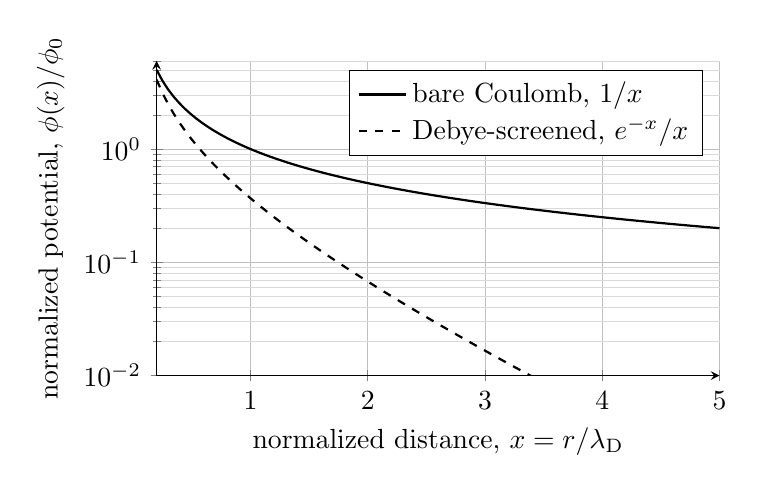
\begin{tikzpicture}
\begin{axis}[
 width=0.72\linewidth,
 height=0.46\linewidth,
 xlabel={normalized distance, $x = r/\lambda_{\mathrm{D}}$},
 ylabel={normalized potential, $\phi(x)/\phi_{0}$},
 ymode=log,
 xmin=0.2, xmax=5,
 ymin=0.01, ymax=6,
 grid=both,
 grid style={line width=0.1pt, draw=gray!30},
 major grid style={line width=0.2pt, draw=gray!50},
 legend pos=north east,
 legend cell align={left},
 axis lines=left,
]
\addplot[black, thick, domain=0.2:5, samples=100] {1/x};
\addlegendentry{bare Coulomb, $1/x$}
\addplot[black, thick, dashed, domain=0.2:5, samples=100] {exp(-x)/x};
\addlegendentry{Debye-screened, $e^{-x}/x$}
\end{axis}
\end{tikzpicture}
\caption{Schematic comparison of the bare-Coulomb potential $1/x$ and the Debye-screened potential $e^{-x}/x$, from Equation~\eqref{eq:screened-potential} in normalized units $x = r/\lambda_{\mathrm{D}}$. The curves are generated from the closed-form expressions only and do not represent measured or simulated data.}
\label{fig:debye-shielding}
\end{figure}

\subsection{The Debye Sphere and the Plasma Parameter}

The Debye length is a genuine screening scale only if enough particles lie within a sphere of radius $\lambda_{\mathrm{D}}$ for the mean-field treatment of Equation~\eqref{ch02-eq:electron-boltzmann} to hold; with only a handful of electrons in this volume, the screened potential would be dominated by discrete fluctuations rather than a smooth collective response. The number of electrons in a Debye sphere,
\begin{equation}
N_{\mathrm{D}} = \frac{4}{3}\pi \lambda_{\mathrm{D}}^{3} n_{\mathrm{e}},
\label{eq:debye-number}
\end{equation}
is the plasma parameter. A plasma in the sense used here is \emph{weakly coupled}, $N_{\mathrm{D}} \gg 1$, so the mean-field description is appropriate. Essentially all sheath, presheath, and ion energy flux theory developed later implicitly assumes this regime, characteristic of laboratory gas discharges and space plasmas.

\section{Characteristic Frequencies and the Formal Criteria for a Plasma}
\label{sec:frequencies}

\subsection{The Electron Plasma Frequency}

Debye shielding describes the static, equilibrium response of a plasma to a fixed perturbation. Its dynamical analogue is the plasma oscillation, whose frequency follows from a simple slab model. Consider a uniform, unmagnetized plasma in which a thin slab of electrons, initially coincident with a corresponding slab of (immobile) ions, is displaced by a small distance $\delta x$ in one dimension. The resulting charge separation produces, by Gauss's law, a uniform restoring field
\begin{equation}
E = \frac{n_{0} e\, \delta x}{\varepsilon_{0}}.
\label{eq:slab-field}
\end{equation}
The equation of motion for an electron of mass $m_{\mathrm{e}}$ in this field is
\begin{equation}
m_{\mathrm{e}}\,\ddot{\delta x} = -eE = -\frac{n_{0} e^{2}}{\varepsilon_{0}}\,\delta x,
\label{eq:slab-eom}
\end{equation}
the equation of a harmonic oscillator with angular frequency
\begin{equation}
\omega_{\mathrm{pe}} = \left(\frac{n_{\mathrm{e}} e^{2}}{\varepsilon_{0} m_{\mathrm{e}}}\right)^{1/2},
\label{eq:plasma-frequency}
\end{equation}
the electron plasma frequency. Physically, $\omega_{\mathrm{pe}}^{-1}$ is the time over which electrons respond to, and screen, a local charge imbalance; comparing Equations~\eqref{ch02-eq:debye-length} and~\eqref{eq:plasma-frequency} gives $\lambda_{\mathrm{D}} = v_{\mathrm{the}}/\omega_{\mathrm{pe}}$, with $v_{\mathrm{the}} = (k_{\mathrm{B}} T_{\mathrm{e}}/m_{\mathrm{e}})^{1/2}$ the electron thermal speed. An analogous ion plasma frequency $\omega_{\mathrm{pi}} = (n_{\mathrm{i}} Z^{2} e^{2}/\varepsilon_{0} m_{\mathrm{i}})^{1/2}$ follows with $m_{\mathrm{i}}$ in place of $m_{\mathrm{e}}$; since $m_{\mathrm{i}} \gg m_{\mathrm{e}}$, $\omega_{\mathrm{pi}} \ll \omega_{\mathrm{pe}}$, and it is $\omega_{\mathrm{pi}}$ that sets the characteristic scales of ion transport across the presheath and sheath \cite{ref0023,ref0665}. The interplay between fast electron response and slower ion dynamics permits a self-consistent, quasi-neutral presheath to be matched onto a non-neutral Debye-scale sheath, examined within the kinetic Tonks--Langmuir model \cite{ref0665,ref0666}.

\subsection{The Cyclotron Frequency}

When a plasma is immersed in a magnetic field of magnitude $B$, a charged particle of charge $q$ and mass $m$ executes circular (or helical) motion about the field line at the cyclotron frequency
\begin{equation}
\omega_{\mathrm{c}} = \frac{|q| B}{m},
\label{eq:cyclotron-frequency}
\end{equation}
with gyroradius $r_{\mathrm{L}} = v_{\perp}/\omega_{\mathrm{c}}$. The electron cyclotron frequency $\omega_{\mathrm{ce}} = eB/m_{\mathrm{e}}$ exceeds the ion value $\omega_{\mathrm{ci}} = eB/m_{\mathrm{i}}$ by the same mass ratio separating $\omega_{\mathrm{pe}}$ from $\omega_{\mathrm{pi}}$. In magnetized discharges relevant to fusion divertors and magnetron sources, the ordering between $\omega_{\mathrm{ci}}$ and the ion presheath transit time determines whether the unmagnetized Bohm criterion applies directly at the sheath edge or must be replaced by the magnetized Chodura criterion, applied at a scale intermediate between $\lambda_{\mathrm{D}}$ and the ion gyroradius \cite{ref0017,ref0018}. The unmagnetized limit, $\omega_{\mathrm{ci}} \to 0$, is the default assumption throughout this monograph.

\subsection{The Three Plasma Criteria}

The distinction between an "ionized gas" and a genuine "plasma" can be stated quantitatively as three conditions, all of which must hold for the collective, quasi-neutral, Debye-screened description above to be self-consistent:
\begin{enumerate}
\item \textbf{Macroscopic scale condition:} $L \gg \lambda_{\mathrm{D}}$, so a bulk region exists over which quasi-neutrality (Equation~\eqref{eq:quasineutrality}) holds and only a thin boundary layer need depart from it.
\item \textbf{Statistical (weak-coupling) condition:} $N_{\mathrm{D}} = \tfrac{4}{3}\pi n_{\mathrm{e}} \lambda_{\mathrm{D}}^{3} \gg 1$ (Equation~\eqref{eq:debye-number}), so collective screening dominates over discrete-particle correlations.
\item \textbf{Collisionality condition:} $\omega_{\mathrm{pe}} \tau \gg 1$, where $\tau$ is the mean time between electron-neutral collisions, so the medium behaves electromagnetically as a plasma rather than an ordinary, collision-dominated gas.
\end{enumerate}
A medium satisfying all three conditions supports the full range of collective plasma phenomena -- shielding, oscillations, and the self-consistent boundary-layer structures central to this monograph. Departures (strongly collisional regimes with $\omega_{\mathrm{pe}}\tau \lesssim 1$, or dusty plasmas with reduced $N_{\mathrm{D}}$) require correspondingly modified sheath and Bohm-criterion treatments \cite{ref0009,ref0024}.

\section{Temperature as a Measure of Energy: Electron and Ion Temperatures}
\label{sec:temperature}

\subsection{Temperature-Energy Equivalence}

In plasma physics, temperature is conventionally expressed directly in energy units by absorbing Boltzmann's constant into the definition, so $k_{\mathrm{B}} T$ is quoted in \si{\joule} or, more commonly, \si{\electronvolt}, with $\SI{1}{\electronvolt} \approx \SI{11604}{\kelvin}$. This reflects that temperature, in a plasma, is best interpreted not as a strict thermodynamic state variable but as a direct measure of the mean random kinetic energy carried by a given species, largely decoupled from that of any other species present. For an isotropic Maxwellian distribution (Section~\ref{sec:distributions}) in three dimensions, equipartition gives a mean kinetic energy of $\tfrac{3}{2} k_{\mathrm{B}} T$ per particle, so $T_{\mathrm{e}}$ and $T_{\mathrm{i}}$ directly measure electron and ion random kinetic energy.

\subsection{Why Electron and Ion Temperatures Differ}

A defining feature of many laboratory plasmas -- central to sheath physics -- is that $T_{\mathrm{e}}$ and $T_{\mathrm{i}}$ are generally unequal, often by one to two orders of magnitude, with $T_{\mathrm{e}} \gg T_{\mathrm{i}}$ typical in low-pressure, weakly ionized discharges. This arises from the enormous electron-ion mass disparity ($m_{\mathrm{i}}/m_{\mathrm{e}} \gtrsim 1836$ even for hydrogen): electrons are accelerated far more efficiently than ions in an applied field, since acceleration for a given force scales as $1/m$, and absorb the bulk of deposited power; and electron-ion energy exchange via elastic collisions is suppressed by $\sim m_{\mathrm{e}}/m_{\mathrm{i}}$ relative to electron-electron or ion-ion thermalization, since collisions between very different masses transfer only a small fraction of kinetic energy per encounter. The electrons thus reach internal thermal equilibrium faster than the electron-ion exchange time, while the colder, weakly coupled ions retain a comparatively low $T_{\mathrm{i}}$, often not far above the neutral gas temperature. It is precisely the large ratio $T_{\mathrm{e}}/T_{\mathrm{i}}$ that lets electrons remain strongly Boltzmann-distributed along the presheath and sheath potential drop while the cold ions accelerate essentially freely -- a separation underlying the classical Bohm sheath criterion \cite{ref0004}.

\subsection{Degrees of Freedom, Pressure, and the Equation of State}

Equipartition assigns a mean energy of $\tfrac{1}{2} k_{\mathrm{B}} T_{s}$ per translational degree of freedom, so the scalar pressure of species $s$, defined kinetically in Equation~\eqref{ch02-eq:moment2} of Section~\ref{sec:distributions}, reduces for an isotropic, three-dimensional population to the ideal-gas-like closure
\begin{equation}
p_{s} = n_{s} k_{\mathrm{B}} T_{s},
\label{eq:equation-of-state}
\end{equation}
applied independently to each species; the total pressure entering force-balance and presheath-acceleration arguments is $p = n_{\mathrm{e}} k_{\mathrm{B}} T_{\mathrm{e}} + \sum_{i} n_{i} k_{\mathrm{B}} T_{i}$. Combined with a polytropic relation $p_{s} \propto n_{s}^{\gamma_{s}}$, the adiabatic index $\gamma_{s}$ distinguishes an isothermal response ($\gamma_{s}=1$, often assumed for electrons) from an adiabatic one ($\gamma_{s}=3$ for one-dimensional ion compression, $\gamma_{s}=5/3$ for three-dimensional adiabatic gas). The assumed $\gamma_{\mathrm{i}}$ for the cold ion fluid alters the predicted ion sound speed and, through it, the Bohm velocity $u_{\mathrm{B}}$ at the sheath edge \cite{ref0023}.

\subsection{Non-Equilibrium (Non-LTE) Plasmas}

A plasma in which $T_{\mathrm{e}} \neq T_{\mathrm{i}}$, and in which excited-state populations are not in Boltzmann equilibrium with either temperature, is termed non-equilibrium, or non-local-thermodynamic-equilibrium (non-LTE). Most low-pressure discharges relevant here -- capacitively and inductively coupled RF discharges, DC glow discharges, Hall-thruster and ion-thruster plasmas -- fall into this category, unlike local-thermodynamic-equilibrium plasmas such as dense arc discharges or stellar interiors, where collisions equilibrate all species to one temperature. Diagnosing $T_{\mathrm{e}}$ and $n_{\mathrm{e}}$ without significant perturbation is a long-standing challenge, addressed by electrostatic (Langmuir) probes, which infer them from the current-voltage characteristic of a small biased electrode \cite{ref0217,ref0194}, and, where probe perturbation is unacceptable, by laser Thomson scattering, measuring them non-invasively from the Doppler-broadened lineshape of scattered light \cite{ref0354,ref0384}. Both diagnostic families recur throughout later chapters, validating sheath and ion energy flux models against independent measurements of the plasma parameters entering those models as boundary conditions.

\section{Velocity Distribution Functions and Their Moments}
\label{sec:distributions}

\subsection{The Kinetic Description}

The most complete non-relativistic description of a plasma species $s$ is its velocity distribution function $f_{s}(\mathbf{r},\mathbf{v},t)$, defined so that $f_{s}(\mathbf{r},\mathbf{v},t)\, \mathrm{d}^{3}r\, \mathrm{d}^{3}v$ is the number of particles of species $s$ in the phase-space volume element $\mathrm{d}^{3}r\, \mathrm{d}^{3}v$ about $(\mathbf{r},\mathbf{v})$. All macroscopic quantities of interest -- density, mean velocity, temperature, pressure, and, central to this monograph, the ion energy flux delivered to a bounding surface -- are velocity-space moments of $f_{s}$. The evolution of $f_{s}$ is governed, absent collisions, by the Vlasov equation, and, with collisions, by the Boltzmann equation \cite{ref0670}, the analytical basis of the kinetic sheath and presheath models discussed later \cite{ref0665,ref0666}.

\subsection{The Maxwellian Distribution}

In thermal equilibrium, or wherever elastic collisions are frequent enough to establish local equilibrium, the velocity distribution of a species with density $n_{s}$, temperature $T_{s}$, and mass $m_{s}$ relaxes to the isotropic Maxwellian form,
\begin{equation}
f_{s}^{\mathrm{M}}(\mathbf{v}) = n_{s}\left(\frac{m_{s}}{2\pi k_{\mathrm{B}} T_{s}}\right)^{3/2} \exp\!\left(-\frac{m_{s} v^{2}}{2 k_{\mathrm{B}} T_{s}}\right),
\label{eq:maxwellian}
\end{equation}
where $v = |\mathbf{v}|$, normalized so $\int f_{s}^{\mathrm{M}}(\mathbf{v})\, \mathrm{d}^{3}v = n_{s}$. A drifting Maxwellian, appropriate for a species with mean flow $\mathbf{u}_{s}$ -- for example, presheath-accelerated ions -- follows from $\mathbf{v} \to \mathbf{v} - \mathbf{u}_{s}$ in the exponent.

\subsection{Moments of the Distribution Function}

The moments of $f_{s}(\mathbf{v})$, obtained by successive multiplication by powers of $v$ and integration over velocity space, generate the fluid variables used throughout plasma theory:
\begin{align}
n_{s} &= \int f_{s}(\mathbf{v})\, \mathrm{d}^{3}v, \label{ch02-eq:moment0}\\
n_{s}\mathbf{u}_{s} &= \int \mathbf{v}\, f_{s}(\mathbf{v})\, \mathrm{d}^{3}v, \label{ch02-eq:moment1}\\
p_{s} = n_{s} k_{\mathrm{B}} T_{s} &= \frac{m_{s}}{3}\int (\mathbf{v}-\mathbf{u}_{s})^{2} f_{s}(\mathbf{v})\, \mathrm{d}^{3}v, \label{ch02-eq:moment2}\\
\mathbf{q}_{s} &= \frac{m_{s}}{2}\int (\mathbf{v}-\mathbf{u}_{s})^{2} (\mathbf{v}-\mathbf{u}_{s})\, f_{s}(\mathbf{v})\, \mathrm{d}^{3}v, \label{eq:moment3}
\end{align}
namely the zeroth (density), first (particle flux and drift velocity), second central (pressure and temperature), and third central (heat flux) moments. This hierarchy is truncated at some order and closed with an equation of state to obtain the fluid (two-fluid) sheath models widely used as tractable alternatives to the full kinetic description \cite{ref0023}.

Of direct relevance here, the one-dimensional ion energy flux delivered to a surface normal to the flow direction $x$ is itself a velocity moment of the ion distribution function evaluated at that surface,
\begin{equation}
\Gamma_{E} = \int_{0}^{\infty} \left(\frac{1}{2} m_{\mathrm{i}} v_{x}^{2}\right) v_{x}\, f_{\mathrm{i}}(v_{x})\, \mathrm{d}v_{x},
\label{eq:energy-flux-preview}
\end{equation}
a weighted third moment of $f_{\mathrm{i}}(v_{x})$ restricted to velocities directed toward the wall. Equation~\eqref{eq:energy-flux-preview} previews the central quantity developed fully in the sheath-theory chapters that follow \cite{ref0672}.

\subsection{Non-Maxwellian Distribution Functions}

The Maxwellian form of Equation~\eqref{eq:maxwellian} is an equilibrium solution of the collisional Boltzmann equation, strictly justified only where collisions are frequent enough to enforce local thermalization. In many plasmas of interest here -- collisionless or weakly collisional low-pressure discharges, the presheath and sheath regions themselves, and RF-driven plasmas subject to stochastic, collisionless electron heating -- the actual distribution departs measurably from Equation~\eqref{eq:maxwellian}. Commonly encountered forms include:
\begin{itemize}
\item \textbf{Bi-Maxwellian distributions}, with distinct effective temperatures parallel and perpendicular to a magnetic field or flow axis, reflecting anisotropic heating.
\item \textbf{Drifting (beam) Maxwellians and superpositions of Maxwellians}, for a bulk thermal population plus a more energetic beam -- e.g., presheath-accelerated ions on a residual thermal population, or a fast secondary-electron beam on a Maxwellian bulk.
\item \textbf{Kappa (generalized Lorentzian) distributions}, Maxwellian-like near $v = 0$ but decaying as a power law rather than exponentially at high velocity, modelling enhanced high-energy tails and their effect on the sheath potential drop and Bohm criterion.
\item \textbf{Two-temperature or depleted-tail EEDFs}, where the bulk follows one effective temperature while the high-energy ionizing tail is depleted or enhanced relative to a single Maxwellian, diagnosed via the Druyvesteyn procedure on the Langmuir probe characteristic \cite{ref0213,ref0217}.
\end{itemize}
Quantities derived under the Maxwellian assumption -- the Bohm velocity, sheath potential drop, and ion energy flux itself -- must, in general, be re-derived from the moments of the actual $f_{s}(v)$ rather than inferred from a single fitted temperature; this motivates treating $f_{\mathrm{i}}(v)$, rather than a single ion temperature, as the fundamental object throughout the ion energy flux formalism developed later. Both electrostatic probes, which can recover the full EEDF \cite{ref0194,ref0226}, and Thomson scattering, whose scattered lineshape directly images the electron velocity distribution \cite{ref0354,ref0384}, are used to characterize such departures.

\section{Collisions, Mean Free Path, and the Degree of Ionization}
\label{sec:collisions}

\subsection{Binary Collisions and the Mean Free Path}

Although the collective, long-range Coulomb interaction qualifies a medium as a plasma, short-range binary collisions -- between charged particles and neutrals, and between charged particles themselves -- remain important for transport coefficients, energy exchange rates, and determining whether the kinetic or fluid description of Section~\ref{sec:distributions} applies in a given region. For particles encountering targets of number density $n_{\mathrm{t}}$ with cross section $\sigma$, the mean free path between collisions is
\begin{equation}
\lambda_{\mathrm{mfp}} = \frac{1}{n_{\mathrm{t}}\,\sigma},
\label{eq:mean-free-path}
\end{equation}
with mean collision frequency $\nu = n_{\mathrm{t}} \sigma \bar{v}$. In a plasma sheath, the ratio of sheath thickness (of order a few $\lambda_{\mathrm{D}}$, or larger in the collisional or Child-Langmuir space-charge-limited regime) to $\lambda_{\mathrm{mfp}}$ determines whether the sheath is collisionless -- ions crossing on ballistic, energy-conserving trajectories -- or collisional, with ion-neutral collisions degrading ion energy and broadening the ion energy distribution at the wall \cite{ref0024,ref0009}. This ratio is one of the principal parameters distinguishing the sheath regimes analysed later, alongside $\lambda_{\mathrm{D}}/L$ from Section~\ref{sec:frequencies}.

\subsection{Elastic, Inelastic, and Coulomb Collisions}

Collisions in a partially ionized plasma fall into several categories. \emph{Elastic} collisions redistribute momentum and kinetic energy without changing internal state, dominating momentum-transfer processes such as ion-neutral and electron-neutral scattering. \emph{Inelastic} collisions transfer energy into internal excitation, dissociation, or ionization of the target, and are the mechanism by which an electron population above $\chi_{\mathrm{ion}}$ (Section~\ref{sec:states-ionization}) sustains the plasma against wall losses. \emph{Coulomb} collisions differ qualitatively: because the $1/r$ potential is long-ranged, a test charge experiences many simultaneous small-angle deflections from distant particles, and these cumulative deflections dominate the effective momentum-transfer cross section. The Rutherford cross section, integrated over impact parameters out to $\lambda_{\mathrm{D}}$ (beyond which the interaction is screened, Section~\ref{ch02-sec:debye}), yields an effective like-species thermal Coulomb collision frequency of the parametric form
\begin{equation}
\nu_{\mathrm{ei}} \sim \frac{n_{\mathrm{e}} e^{4} \ln\Lambda}{4\pi\varepsilon_{0}^{2} m_{\mathrm{e}}^{2} v_{\mathrm{the}}^{3}},
\label{eq:coulomb-frequency}
\end{equation}
where $\ln\Lambda = \ln(\lambda_{\mathrm{D}}/b_{0})$ is the Coulomb logarithm and $b_{0}$ the classical distance of closest approach; without a Debye-screened outer cutoff, the small-angle Coulomb collision rate would formally diverge. In weakly ionized, low-temperature discharges, electron-neutral and ion-neutral collisions dominate over electron-ion Coulomb collisions owing to the low degree of ionization $\alpha$ (Equation~\eqref{eq:ionization-degree}), whereas in fully ionized fusion and space plasmas the ordering reverses.

\subsection{Degree of Ionization}

The degree of ionization of a partially ionized gas, containing free electrons and ions at density $n_{\mathrm{e}} \approx Z n_{\mathrm{i}}$ together with a residual neutral background at density $n_{\mathrm{n}}$, is defined as
\begin{equation}
\alpha \equiv \frac{n_{\mathrm{i}}}{n_{\mathrm{i}} + n_{\mathrm{n}}}.
\label{eq:ionization-degree}
\end{equation}
A plasma is \emph{weakly ionized} when $\alpha \ll 1$, so collisions with the neutral background dominate (electron-neutral collisions controlling energy balance and transport; ion-neutral collisions controlling ion momentum loss and sheath collisionality), and \emph{fully} or \emph{strongly ionized} when $\alpha \to 1$, so Coulomb collisions among charged species dominate. Most low-pressure discharges here operate weakly ionized, typically $\alpha \sim 10^{-6}$--$10^{-2}$, whereas fusion edge and scrape-off-layer plasmas, and many electric-propulsion devices, approach or reach the fully ionized regime. In thermal equilibrium, $\alpha$ is governed by the Saha equation, depending exponentially on $\chi_{\mathrm{ion}}/k_{\mathrm{B}} T$; but because most laboratory low-temperature plasmas are strongly non-equilibrium (Section~\ref{sec:temperature}), $\alpha$ is instead set kinetically, by electron-impact ionization balanced against transport losses to the walls, and can differ from the Saha value by many orders of magnitude.

\subsection{Collisionality Regimes and Sheath Classification}

The interplay between the mean free path of Equation~\eqref{eq:mean-free-path} and the relevant length scales -- $\lambda_{\mathrm{D}}$, the presheath length, and the sheath thickness -- provides a natural classification of sheath regimes. In the \emph{collisionless} limit, $\lambda_{\mathrm{mfp}} \gg$ sheath and presheath length scales, ions cross the entire plasma-wall transition without a collision, so their velocity distribution at the wall is determined entirely by the potential profile and the distribution function at the sheath edge -- a regime amenable to exact kinetic (Vlasov) treatment \cite{ref0013,ref0665}. In the opposite, strongly \emph{collisional} limit, ion-neutral collisions occur many times as an ion crosses the presheath and sheath, degrading its directed kinetic energy and driving the ion velocity distribution toward a mobility-limited, drift-diffusion form; this requires a fundamentally different fluid-collisional treatment of both the Bohm criterion and the resulting ion energy flux \cite{ref0024,ref0009}. Intermediate regimes, with a handful of collisions across the presheath but an effectively collisionless sheath, are common and have motivated hybrid kinetic-fluid treatments \cite{ref0012}. Laser-induced fluorescence measurements of the ion velocity distribution in the presheath provide one of the few direct experimental windows onto this classification \cite{ref0292}.

\section{Classification of Laboratory and Technological Plasmas}
\label{sec:classification}

The concepts developed in this chapter -- density, temperature, degree of ionization, and collisionality -- span an enormous range of values across the laboratory and natural plasmas studied in the literature. Table~\ref{tab:plasma-classification} collects representative, order-of-magnitude parameter ranges for several plasma types directly relevant to the ion energy flux and sheath problems addressed here. The entries are illustrative, rounded ranges assembled for orientation only, not measured or reported values for any specific device; actual operating parameters can lie outside the indicated ranges.

\begin{table}[htbp]
\centering
\caption{Illustrative, order-of-magnitude classification of common laboratory and technological plasmas by electron density and electron temperature. Ranges are representative and schematic, intended for orientation only, and are not measured or experimentally reported data.}
\label{tab:plasma-classification}
\begin{tabular}{@{}llll@{}}
\toprule
Plasma type & $n_{\mathrm{e}}$ (\si{\per\cubic\meter}) & $T_{\mathrm{e}}$ (\si{\electronvolt}) & Typical $\alpha$ \\
\midrule
DC glow discharge & \num{e14}--\num{e17} & 1--5 & weakly ionized \\
Capacitively coupled RF plasma & \num{e14}--\num{e17} & 1--5 & weakly ionized \\
Inductively coupled RF plasma & \num{e16}--\num{e19} & 2--8 & weakly ionized \\
Hall-thruster discharge channel & \num{e17}--\num{e19} & 10--40 & moderately ionized \\
Tokamak edge / scrape-off layer & \num{e18}--\num{e20} & 10--100 & strongly ionized \\
Earth ionosphere (F region) & \num{e10}--\num{e12} & $\sim$0.1 & weakly ionized \\
\bottomrule
\end{tabular}
\end{table}

The table underscores a recurring theme: sheath and ion energy flux theory, developed for a generic quasi-neutral plasma bounded by a wall, must in practice be specialized to the collisionality, magnetization, and degree of ionization of the specific device under consideration. Capacitively coupled RF discharges, in particular, occupy a regime of especially rich, time-dependent sheath dynamics, and constitute one of the principal application contexts examined later. Diagnostic access to $n_{\mathrm{e}}$ and $T_{\mathrm{e}}$ across this range has historically relied on electrostatic (Langmuir) probes at the lower-density end \cite{ref0194,ref0217} and, where probe survivability is problematic, on Thomson scattering at higher densities and temperatures, including fusion and electric-propulsion plasmas \cite{ref0354,ref0355}.

\section{Summary}
\label{sec:fundamentals-summary}

This chapter established the foundation for the sheath and ion energy flux theory that follows. A plasma was defined as a quasi-neutral, collectively responding ionized gas, distinguished from a merely ionized gas by three criteria: a system size large compared with the Debye length, many particles within a Debye sphere, and a plasma oscillation frequency large compared with the collision rate with neutrals. The Debye length was derived from the linearized Poisson-Boltzmann equation, yielding the exponentially screened potential of Equation~\eqref{eq:screened-potential} and the length scale over which quasi-neutrality is broken -- precisely the scale on which the plasma sheath forms. The electron and ion plasma frequencies were derived from a slab oscillation model, and the cyclotron frequency was introduced for the magnetized case relevant to later generalizations of the Bohm criterion. Temperature was interpreted as a direct measure of random kinetic energy per particle, and the large $T_{\mathrm{e}}/T_{\mathrm{i}}$ disparity typical of non-equilibrium plasmas was traced to the electron-ion mass ratio. The velocity distribution function $f_{s}(v)$ and its moments -- density, flow velocity, pressure and temperature, and heat flux -- were introduced as the kinetic description underlying every fluid quantity used later, and the ion energy flux $\Gamma_{E}$ was previewed as a weighted moment of $f_{\mathrm{i}}(v)$, Equation~\eqref{eq:energy-flux-preview}. Departures from the Maxwellian form -- bi-Maxwellian, drifting, kappa, and depleted-tail distributions -- were surveyed together with the diagnostics, electrostatic probes and Thomson scattering, used to characterize them. Finally, collisions were quantified through the mean free path and degree of ionization, giving the collisionless/intermediate/collisional classification that organizes much of the sheath-theory literature revisited later, and a representative table situated the ion energy flux problem within the broader landscape of plasma types to which it applies. With these fundamentals in place, the chapter that follows turns to the plasma-wall transition itself: the presheath, the Bohm criterion, and the sheath proper.

\chapter{Theory of the Plasma Sheath}
\label{ch:sheath}

Every laboratory or technological plasma is bounded by a material surface, and it is at that boundary that the plasma communicates its energy, particle, and momentum content to the outside world. The layer that mediates this communication is the \emph{sheath}: a thin, non-neutral region, typically a few to a few tens of Debye lengths thick, in which the plasma potential collapses from its quasineutral bulk value to the (generally more negative) value imposed by the wall. Because essentially all of the potential drop between the plasma interior and a solid boundary occurs across this narrow layer, the sheath determines the energy with which ions strike a surface -- the ion energy flux $\Gamma_{E}$ this monograph quantifies. This chapter develops sheath theory from first principles: why a sheath must exist, the Bohm criterion and presheath that enforce it, the space-charge-limited sheath structure (matrix and Child--Langmuir limits), its generalization to collisional and magnetized plasmas (the Bohm--Chodura criterion), its time-dependent behaviour under RF excitation, and the kinetic and finite-Debye-length corrections that refine the fluid picture. The notation $T_{\mathrm{e}}$, $T_{\mathrm{i}}$, $n_{\mathrm{e}}$, $n_{\mathrm{i}}$, $\lambda_{\mathrm{D}}$, $u_{\mathrm{B}}$, $\Gamma_{E}$, $f_{\mathrm{i}}(v)$ is used consistently throughout.

\section{Why a Sheath Forms: Differential Mobility and Flux Balance}

\subsection{The disparity in thermal velocities}

The physical origin of the sheath lies in the disparity between electron and ion thermal velocities in a weakly ionized, low-temperature plasma. For a Maxwellian species of mass $m$ and temperature $T$, the mean thermal speed is
\begin{equation}
\bar{v} = \sqrt{\frac{8 k_{\mathrm{B}} T}{\pi m}},
\end{equation}
and the random one-sided flux incident on a plane surface from an isotropic Maxwellian distribution is $\Gamma = \tfrac{1}{4} n \bar{v}$. Because $m_{\mathrm{i}} \gg m_{\mathrm{e}}$ (a factor of $\num{1836}$ for hydrogen, up to $\sim \num{2.4e5}$ for xenon) and $T_{\mathrm{e}} \gtrsim T_{\mathrm{i}}$ in most laboratory discharges, electrons are vastly more mobile than ions. If a plasma with $n_{\mathrm{e}} = n_{\mathrm{i}}$ were suddenly placed in contact with a floating or grounded wall, the initial electron flux would exceed the ion flux by a factor of order $\sqrt{m_{\mathrm{i}}/m_{\mathrm{e}}}$, two to three orders of magnitude -- the starting point for essentially every treatment of the plasma-sheath transition \cite{ref0013,ref0015}.

\subsection{Charge accumulation and the self-consistent field}

Because electrons escape to the wall far faster than ions, the wall rapidly accumulates net negative charge, while the adjacent plasma is left correspondingly positive as it is depleted of electrons. The resulting field points from the quasineutral bulk toward the wall, decelerating fast electrons and accelerating slow ions, until a steady state is reached in which the depressed electron flux balances the enhanced ion flux. The layer that carries this field, and the compensating charge deficit required by Poisson's equation, is the sheath -- a direct consequence of flux balance under a large electron-to-ion mobility ratio.

\subsection{Quasineutrality breakdown and the natural length scale}

In the bulk plasma, quasineutrality ($n_{\mathrm{e}} \simeq n_{\mathrm{i}}$) is maintained to high precision: any local charge imbalance $\delta n = n_{\mathrm{i}} - n_{\mathrm{e}}$ produces, through Poisson's equation,
\begin{equation}
\nabla^{2} \phi = -\frac{e\,\delta n}{\varepsilon_{0}},
\end{equation}
a restoring field acting on a length scale set by the electron Debye length,
\begin{equation}
\lambda_{\mathrm{D}} = \left( \frac{\varepsilon_{0} k_{\mathrm{B}} T_{\mathrm{e}}}{n_{\mathrm{e}} e^{2}} \right)^{1/2}.
\label{ch03-eq:debye-length}
\end{equation}
Over distances much larger than $\lambda_{\mathrm{D}}$ the plasma shields out imposed potential perturbations and remains quasineutral; on distances comparable to or smaller than $\lambda_{\mathrm{D}}$, quasineutrality can fail, since the electrostatic energy of charge separation becomes comparable to the particle thermal energy. The sheath is where this failure is enforced by the boundary condition itself: the wall must absorb net negative charge to establish the retarding potential that balances the fluxes, so Poisson's equation requires $n_{\mathrm{i}} > n_{\mathrm{e}}$ throughout. The natural thickness of this layer is of order a few $\lambda_{\mathrm{D}}$ in the simplest (``matrix'') approximation, growing super-linearly with voltage once ion space charge is treated self-consistently (the Child--Langmuir regime) \cite{ref0012,ref0024}.

\section{Plasma, Wall, and Floating Potentials}

\subsection{Definitions and the current-balance framework}

Three potentials organize the discussion of any bounded plasma. The \emph{plasma potential} $V_{\mathrm{p}}$ is the potential of the quasineutral bulk, the reference for all sheath potential drops. The \emph{wall potential} $V_{\mathrm{w}}$ is the potential actually acquired by the bounding surface, depending on whether it is floating, grounded, or externally biased. The \emph{floating potential} $V_{\mathrm{f}}$ is the special case realized when the surface draws no net current -- the condition defining a probe or any unbiased dielectric wall. In all cases the physics is governed by the total current density delivered to the surface,
\begin{equation}
J(V_{\mathrm{w}}) = J_{\mathrm{i}}(V_{\mathrm{w}}) - J_{\mathrm{e}}(V_{\mathrm{w}}),
\end{equation}
with $J_{\mathrm{i}}$ and $J_{\mathrm{e}}$ both defined positive when directed toward the wall.

\subsection{Ion and electron current density at the surface}

The ion current density delivered to the wall is fixed by the flux of ions crossing the sheath edge -- set by the Bohm criterion of Section~\ref{ch03-sec:bohm}, essentially independent of $V_{\mathrm{w}}$ provided $V_{\mathrm{w}} < V_{\mathrm{p}}$:
\begin{equation}
J_{\mathrm{i}} = e\, n_{\mathrm{s}}\, u_{\mathrm{B}}, \qquad u_{\mathrm{B}} = \sqrt{\frac{k_{\mathrm{B}} T_{\mathrm{e}}}{m_{\mathrm{i}}}},
\label{eq:bohm-flux}
\end{equation}
where $n_{\mathrm{s}}$ is the sheath-edge density and $u_{\mathrm{B}}$ the Bohm speed. The electron current, by contrast, is exponentially sensitive to the retarding potential, since only the high-energy tail with $\tfrac12 m_{\mathrm{e}} v^{2} \geq e|V_{\mathrm{p}} - V_{\mathrm{w}}|$ surmounts the barrier:
\begin{equation}
J_{\mathrm{e}}(V_{\mathrm{w}}) = \frac{1}{4} e\, n_{\mathrm{s}} \bar{v}_{\mathrm{e}} \exp\!\left[ \frac{e (V_{\mathrm{w}} - V_{\mathrm{p}})}{k_{\mathrm{B}} T_{\mathrm{e}}} \right], \qquad \bar{v}_{\mathrm{e}} = \sqrt{\frac{8 k_{\mathrm{B}} T_{\mathrm{e}}}{\pi m_{\mathrm{e}}}}.
\label{eq:electron-retarded-flux}
\end{equation}
This exponential form recurs in the presheath and is central to virtually every fluid derivation of the Bohm criterion \cite{ref0013}.

\subsection{The floating condition}

The floating potential is obtained by setting $J = 0$, i.e.\ equating the retarded electron flux of Eq.~\eqref{eq:electron-retarded-flux} to the Bohm ion flux of Eq.~\eqref{eq:bohm-flux}:
\begin{equation}
\frac{1}{4} \bar{v}_{\mathrm{e}} \exp\!\left[ \frac{e (V_{\mathrm{f}} - V_{\mathrm{p}})}{k_{\mathrm{B}} T_{\mathrm{e}}} \right] = u_{\mathrm{B}}.
\end{equation}
Solving for the sheath potential drop gives the classical floating-potential formula
\begin{equation}
V_{\mathrm{f}} - V_{\mathrm{p}} = -\frac{k_{\mathrm{B}} T_{\mathrm{e}}}{2e} \ln\!\left( \frac{m_{\mathrm{i}}}{2\pi m_{\mathrm{e}}} \right).
\label{eq:floating-potential}
\end{equation}
Because $m_{\mathrm{i}}/m_{\mathrm{e}} \gg 1$ for any real ion, the logarithm is positive and of order $5$--$10$, so the floating surface always sits several electron temperatures below the plasma potential. Table~\ref{tab:floating-potentials} lists the normalized offset for several ion species; it grows slowly (logarithmically) with ion mass.

\begin{table}[htbp]
\centering
\caption{Normalized floating-potential offset $-(V_{\mathrm{f}} - V_{\mathrm{p}})/T_{\mathrm{e}}$ from Eq.~\eqref{eq:floating-potential} for representative singly ionized species (cold-ion limit, $T_{\mathrm{i}} \to 0$); values are illustrative, computed from the analytic formula, not measurements.}
\label{tab:floating-potentials}
\begin{tabular}{lcc}
\toprule
Ion species & $m_{\mathrm{i}}/m_{\mathrm{e}}$ & $-(V_{\mathrm{f}}-V_{\mathrm{p}})/T_{\mathrm{e}}$ \\
\midrule
Hydrogen (H$^{+}$) & $1.84\times10^{3}$ & $2.84$ \\
Helium (He$^{+}$) & $7.34\times10^{3}$ & $3.53$ \\
Argon (Ar$^{+}$) & $7.34\times10^{4}$ & $4.68$ \\
Xenon (Xe$^{+}$) & $2.41\times10^{5}$ & $5.28$ \\
\bottomrule
\end{tabular}
\end{table}

For $V_{\mathrm{w}} < V_{\mathrm{f}}$, the ion current saturates at the Bohm value while the electron current falls exponentially -- the regime governing ion energy delivered to any negatively biased surface.

\subsection{Grounded and biased surfaces}

When $V_{\mathrm{w}}$ is fixed externally -- a grounded electrode, a DC- or RF-biased substrate -- the net current need not vanish, and $V_{\mathrm{p}} - V_{\mathrm{w}}$ becomes the controlling parameter for ion bombardment energy. Since this drop occurs almost entirely across the sheath (the presheath drop being only $T_{\mathrm{e}}/2e$), an ion entering at $u_{\mathrm{B}}$ and falling through the full sheath potential arrives with kinetic energy
\begin{equation}
E_{\mathrm{i}} \simeq \frac{1}{2} m_{\mathrm{i}} u_{\mathrm{B}}^{2} + e\left(V_{\mathrm{p}} - V_{\mathrm{w}}\right) = \frac{1}{2} k_{\mathrm{B}} T_{\mathrm{e}} + e\left(V_{\mathrm{p}} - V_{\mathrm{w}}\right),
\label{eq:ion-impact-energy}
\end{equation}
in the collisionless, unidirectional limit. Equation~\eqref{eq:ion-impact-energy} is the fundamental link between sheath theory and the ion energy flux $\Gamma_{E} = \Gamma_{\mathrm{i}} E_{\mathrm{i}}$ this monograph quantifies, and is refined below to account for collisions, magnetization, time dependence, and the finite spread of $f_{\mathrm{i}}(v)$.

\subsection{The ion energy flux as a moment of the sheath-edge distribution}

Given the ion velocity distribution $f_{\mathrm{i}}(v)$ at any plane of interest -- most usefully the wall -- the ion particle flux and ion energy flux are the zeroth and energy-weighted first moments of $f_{\mathrm{i}}(v)$:
\begin{equation}
\Gamma_{\mathrm{i}} = \int_{0}^{\infty} v\, f_{\mathrm{i}}(v)\, \mathrm{d}v, \qquad \Gamma_{E} = \int_{0}^{\infty} \left( \frac{1}{2} m_{\mathrm{i}} v^{2} \right) v\, f_{\mathrm{i}}(v)\, \mathrm{d}v.
\label{eq:energy-flux-moments}
\end{equation}
In the idealized cold-ion, collisionless, unmagnetized, DC limit, $f_{\mathrm{i}}(v)$ collapses to a delta function at the impact speed of Eq.~\eqref{eq:ion-impact-energy}, and Eq.~\eqref{eq:energy-flux-moments} reduces to $\Gamma_{E} = \Gamma_{\mathrm{i}} E_{\mathrm{i}}$. Every generalization treated below -- collisional broadening, the Bohm--Chodura conditions, the bimodal RF distribution, and the kinetic Bohm criterion of Eq.~\eqref{eq:kinetic-bohm} -- broadens, skews, or splits $f_{\mathrm{i}}(v)$ away from this delta function, decoupling $\Gamma_{E}$ from the simple product of mean flux and mean energy. Because $\Gamma_{E}$ weights by an extra factor of $v^{2}$, it is disproportionately sensitive to the high-energy tail of $f_{\mathrm{i}}(v)$, in contrast to the kinetic Bohm criterion (Section~\ref{ch03-sec:bohm}), whose $v^{-2}$ weighting makes it sensitive to the low-energy tail: a population can satisfy the marginal Bohm condition comfortably in bulk while its low-velocity tail threatens it, yet deliver an energy flux dominated by a high-velocity tail representing a small fraction of the total flux. Quantifying $\Gamma_{E}$ accurately therefore requires the full shape of $f_{\mathrm{i}}(v)$, not merely the mean sheath voltage and Bohm flux.

\section{The Bohm Criterion and the Presheath}
\label{ch03-sec:bohm}

\subsection{Statement and fluid model}

The Bohm criterion is the single most important quantitative result in sheath theory: ions cannot enter a sheath at rest, or even at an arbitrary subsonic drift, but must arrive at the sheath edge with directed velocity at least the ion acoustic (Bohm) speed $u_{\mathrm{B}} = \sqrt{k_{\mathrm{B}} T_{\mathrm{e}}/m_{\mathrm{i}}}$, first obtained by Bohm and later elaborated into kinetic, collisional, multi-species, and magnetized forms \cite{ref0001,ref0004}. It follows from requiring a monotonic, physically admissible space-charge solution of Poisson's equation between the quasineutral plasma and the strongly non-neutral sheath.

Consider a one-dimensional, steady-state, cold-ion fluid model: ions are created far from the wall and fall collisionlessly and unmagnetized through the presheath and sheath, while electrons, Maxwellian at $T_{\mathrm{e}}$, obey the Boltzmann relation at every point:
\begin{equation}
n_{\mathrm{e}}(\phi) = n_{0} \exp\!\left( \frac{e \phi}{k_{\mathrm{B}} T_{\mathrm{e}}} \right),
\label{ch03-eq:electron-boltzmann}
\end{equation}
where $\phi \le 0$ is the local potential relative to the field-free interior and $n_{0}$ the unperturbed bulk density. Ion continuity and cold-ion momentum conservation give
\begin{align}
n_{\mathrm{i}}(x)\, u_{\mathrm{i}}(x) &= \Gamma_{\mathrm{i}} = n_{0} u_{0}, \label{eq:ion-continuity}\\
\frac{1}{2} m_{\mathrm{i}} u_{\mathrm{i}}^{2}(x) &= \frac{1}{2} m_{\mathrm{i}} u_{0}^{2} - e \phi(x), \label{eq:ion-energy}
\end{align}
where $u_{0}$ is the ion drift speed at the presheath--sheath reference point $\phi=0$. Combining these yields the ion density profile
\begin{equation}
n_{\mathrm{i}}(\phi) = \frac{n_{0} u_{0}}{\sqrt{u_{0}^{2} - 2 e \phi/m_{\mathrm{i}}}}.
\label{eq:ion-density-profile}
\end{equation}

\subsection{Poisson's equation and the marginal stability argument}

The self-consistent potential must satisfy Poisson's equation with the two charge densities of Eqs.~\eqref{ch03-eq:electron-boltzmann} and~\eqref{eq:ion-density-profile}:
\begin{equation}
\varepsilon_{0} \frac{\mathrm{d}^{2} \phi}{\mathrm{d} x^{2}} = e \left[ n_{\mathrm{e}}(\phi) - n_{\mathrm{i}}(\phi) \right] = e n_{0} \left[ \exp\!\left(\frac{e\phi}{k_{\mathrm{B}} T_{\mathrm{e}}}\right) - \frac{u_{0}}{\sqrt{u_{0}^{2} - 2e\phi/m_{\mathrm{i}}}} \right].
\label{ch03-eq:poisson-full}
\end{equation}
For a physically sensible solution, in which $\phi$ decreases monotonically from $0$ to a negative wall value, the right-hand side must be non-negative for all $\phi\le0$ near $\phi=0$. Expanding both terms to first order in $\phi$,
\begin{align}
n_{\mathrm{e}}(\phi) &\approx n_{0}\left(1 + \frac{e\phi}{k_{\mathrm{B}} T_{\mathrm{e}}}\right), &
n_{\mathrm{i}}(\phi) &\approx n_{0}\left(1 + \frac{e\phi}{m_{\mathrm{i}} u_{0}^{2}}\right),
\end{align}
and substituting into Eq.~\eqref{ch03-eq:poisson-full}, the linear term gives
\begin{equation}
\varepsilon_{0} \frac{\mathrm{d}^{2}\phi}{\mathrm{d} x^{2}} \approx e n_{0}\, \phi\left( \frac{1}{k_{\mathrm{B}} T_{\mathrm{e}}} - \frac{1}{m_{\mathrm{i}} u_{0}^{2}} \right).
\label{eq:linearized-poisson}
\end{equation}
Since $\phi\le0$, the bracketed term must be non-negative for net positive space charge:
\begin{equation}
\frac{1}{k_{\mathrm{B}} T_{\mathrm{e}}} \ge \frac{1}{m_{\mathrm{i}} u_{0}^{2}} \qquad \Longleftrightarrow \qquad u_{0}^{2} \ge \frac{k_{\mathrm{B}} T_{\mathrm{e}}}{m_{\mathrm{i}}},
\end{equation}
which on taking the square root gives the Bohm criterion,
\begin{equation}
\boxed{\, u_{0} \ge u_{\mathrm{B}} \equiv \sqrt{\frac{k_{\mathrm{B}} T_{\mathrm{e}}}{m_{\mathrm{i}}}} \,}.
\label{ch03-eq:bohm-criterion}
\end{equation}
Eq.~\eqref{ch03-eq:bohm-criterion} is a marginal (inequality) condition rather than an exact equality: if $u_0 < u_{\mathrm B}$, no monotonic space-charge solution exists; if $u_0 = u_{\mathrm B}$ exactly, the linear term vanishes and higher-order terms must sustain the field, producing a formally singular ion density gradient at the sheath edge.

\subsection{Physical interpretation}

The Bohm criterion can be read as a statement about the relative stiffness of ion and electron responses to a potential perturbation. From Eq.~\eqref{eq:linearized-poisson}, $1/(m_{\mathrm{i}} u_{0}^{2})$ is the ion compressibility response and $1/(k_{\mathrm{B}} T_{\mathrm{e}})$ the electron (Boltzmann) response to the same $\phi$. When ions are slow, a small negative $\phi$ compresses the ion fluid more strongly than it depletes the electrons, so $n_{\mathrm{i}} > n_{\mathrm{e}}$ is never achieved; once ions move fast enough, further deceleration produces only a small density increase, while the exponential electron response keeps depleting $n_{\mathrm{e}}$, letting the required space charge build. The Bohm speed is thus the threshold ion drift at which the ion fluid becomes ``stiff'' enough, relative to the electrons, to support a stable non-neutral transition.

\subsection{The presheath}

The Bohm criterion demands that ions arrive at the sheath edge already moving at $u_{\mathrm{B}}$, yet ions are typically born by ionization essentially at rest. The region that performs this acceleration is the \emph{presheath}: a quasineutral region, generally many Debye lengths in extent, supporting a weak field that accelerates ions from rest up to $u_{\mathrm{B}}$ while remaining quasineutral to good approximation \cite{ref0006,ref0013}. The total presheath potential drop follows from Eq.~\eqref{eq:ion-energy} between the field-free source ($u\approx0$) and the sheath edge ($u=u_{\mathrm{B}}$):
\begin{equation}
e \left| \Delta \phi_{\mathrm{presheath}} \right| = \frac{1}{2} m_{\mathrm{i}} u_{\mathrm{B}}^{2} = \frac{1}{2} k_{\mathrm{B}} T_{\mathrm{e}} \qquad \Longrightarrow \qquad \Delta\phi_{\mathrm{presheath}} = -\frac{k_{\mathrm{B}} T_{\mathrm{e}}}{2e}.
\label{eq:presheath-drop}
\end{equation}
This universal result -- a presheath drop of exactly $T_{\mathrm{e}}/2$ for cold, unmagnetized, collisionless ions born at rest -- is a direct corollary of the Bohm criterion \cite{ref0013,ref0023}. The associated sheath-edge density reduction follows from Eq.~\eqref{ch03-eq:electron-boltzmann}: $n_{\mathrm{s}} = n_{0} \exp(-1/2) \approx 0.61\, n_{0}$, a factor used throughout plasma diagnostics to relate a bulk density measurement to the flux delivered to a wall.

The presheath/sheath boundary is not a sharp physical division but a matter of scale separation -- the presheath varies on the ionization or collisional mean free path, the sheath on the Debye length -- formally distinct only as $\lambda_{\mathrm{D}} \to 0$; what condition to impose at the notional sheath edge remains debated.

\section{Sheath Structure and Thickness}

\subsection{Debye-length scaling of the collisionless sheath}

Once ions cross the sheath edge at $u_{\mathrm{B}}$, they enter a region where quasineutrality is abandoned and the full nonlinear Poisson equation, Eq.~\eqref{ch03-eq:poisson-full}, governs the potential profile. Two limiting, tractable descriptions are standard: the \emph{matrix sheath}, appropriate to an initial transient or order-of-magnitude estimate, and the \emph{Child--Langmuir sheath}, appropriate to a steady, voltage-driven sheath where ion density has fallen substantially by the wall. Both predict a thickness of order a few Debye lengths for $V_{0} \sim T_{\mathrm{e}}$, growing as a power of the voltage at larger bias \cite{ref0012,ref0024}.

\subsection{The matrix sheath}

The matrix-sheath approximation sets $n_{\mathrm{i}}(x) = n_{\mathrm{s}}$ uniformly and neglects the electron density ($n_{\mathrm{e}} \approx 0$, exponentially small once $|\phi| \gg T_{\mathrm{e}}/e$). Poisson's equation becomes linear in $x$:
\begin{equation}
\varepsilon_{0} \frac{\mathrm{d}^{2}\phi}{\mathrm{d}x^{2}} = -e\, n_{\mathrm{s}}.
\end{equation}
Taking the sheath edge at $x=0$ with $\phi(0)=0$ and $\mathrm{d}\phi/\mathrm{d}x|_{x=0}=0$, integration gives
\begin{equation}
\phi(x) = -\frac{e n_{\mathrm{s}}}{2\varepsilon_{0}} x^{2}.
\end{equation}
Setting $\phi(s) = -V_{0}$ at the wall ($V_{0} = V_{\mathrm{p}} - V_{\mathrm{w}} > 0$) and solving for $s$ gives the matrix-sheath thickness
\begin{equation}
s_{\mathrm{matrix}} = \left( \frac{2 \varepsilon_{0} V_{0}}{e n_{\mathrm{s}}} \right)^{1/2} = \lambda_{\mathrm{Ds}} \left( \frac{2 e V_{0}}{k_{\mathrm{B}} T_{\mathrm{e}}} \right)^{1/2},
\label{eq:matrix-sheath}
\end{equation}
where $\lambda_{\mathrm{Ds}} = (\varepsilon_{0} k_{\mathrm{B}} T_{\mathrm{e}} / n_{\mathrm{s}} e^{2})^{1/2}$ is the Debye length at the sheath-edge density: a few Debye lengths for $V_{0}$ of order a few $T_{\mathrm{e}}$, growing only as the square root of the applied voltage.

\subsection{The Child--Langmuir sheath}

The matrix approximation over-estimates ion density (and under-estimates thickness) at large voltage, since it ignores that ions accelerate substantially crossing the sheath, so $n_{\mathrm{i}}(x)$ must fall with distance to keep $\Gamma_{\mathrm{i}} = n_{\mathrm{i}} u_{\mathrm{i}}$ constant. Retaining this gives the space-charge-limited, or Child--Langmuir, sheath. With $x=0$, $\phi(0)=0$, and $u_{\mathrm{i}}(0)=u_{\mathrm{B}}$ (negligible for $V_0 \gg T_{\mathrm{e}}/e$, dropped below), current continuity and energy conservation give
\begin{equation}
J_{\mathrm{i}} = e\, n_{\mathrm{i}}(x)\, u_{\mathrm{i}}(x) = \text{const}, \qquad \frac{1}{2} m_{\mathrm{i}} u_{\mathrm{i}}^{2}(x) = -e\phi(x) \equiv e\,\psi(x),
\end{equation}
with $\psi \equiv -\phi \ge 0$ rising monotonically from $0$ at the sheath edge to $V_{0}$ at the wall. Eliminating $u_{\mathrm{i}}$ gives $n_{\mathrm{i}}(x) = J_{\mathrm{i}} / [e \sqrt{2e\psi/m_{\mathrm{i}}}\,]$, and neglecting the electron density in the sheath interior, Poisson's equation becomes
\begin{equation}
\varepsilon_{0} \frac{\mathrm{d}^{2}\psi}{\mathrm{d}x^{2}} = J_{\mathrm{i}} \sqrt{\frac{m_{\mathrm{i}}}{2 e \psi}}.
\label{eq:cl-ode}
\end{equation}
Integrating once (with $\mathrm{d}\psi/\mathrm{d}x=0$ at $x=0$) gives $\mathrm{d}\psi/\mathrm{d}x = \left[ (4 J_{\mathrm{i}}/\varepsilon_{0}) \sqrt{m_{\mathrm{i}}/2e} \right]^{1/2} \psi^{1/4}$; integrating again from $\psi=0$ at $x=0$ gives $\tfrac{4}{3}\psi^{3/4} = \left[ (4J_{\mathrm{i}}/\varepsilon_{0})\sqrt{m_{\mathrm{i}}/2e} \right]^{1/2} x$. Evaluating at the wall, $\psi(s)=V_{0}$, and solving for $J_{\mathrm{i}}$ gives the \textbf{Child--Langmuir law}:
\begin{equation}
\boxed{\, J_{\mathrm{i}} = \frac{4}{9}\, \varepsilon_{0} \sqrt{\frac{2e}{m_{\mathrm{i}}}}\, \frac{V_{0}^{3/2}}{s^{2}} \,}.
\label{ch03-eq:child-langmuir}
\end{equation}
This is the classical space-charge-limited current law of a planar vacuum diode, applied here to the ion current crossing a collisionless plasma sheath \cite{ref0012,ref0024}. Since $J_{\mathrm{i}} \propto V_{0}^{3/2}/s^{2}$, for a fixed Bohm current $J_{\mathrm{i}} = e n_{\mathrm{s}} u_{\mathrm{B}}$, increasing $V_{0}$ must be accompanied by increasing $s$; substituting and solving for $s$ gives
\begin{equation}
s_{\mathrm{CL}} = \left( \frac{4\sqrt{2}}{9} \right)^{1/2} \lambda_{\mathrm{Ds}} \left( \frac{e V_{0}}{k_{\mathrm{B}} T_{\mathrm{e}}} \right)^{3/4} \approx 0.79\, \lambda_{\mathrm{Ds}} \left( \frac{e V_{0}}{k_{\mathrm{B}} T_{\mathrm{e}}} \right)^{3/4}.
\label{eq:cl-thickness}
\end{equation}
The Child--Langmuir sheath thus grows as $(V_{0}/T_{\mathrm{e}})^{3/4}$, faster than the $(V_{0}/T_{\mathrm{e}})^{1/2}$ matrix scaling, since a current-conserving sheath must spread its ion space charge over a larger volume as ions accelerate to increasingly rarefied speeds. Figure~\ref{fig:child-langmuir-profile} shows the normalized potential profile implied by this solution.

\begin{figure}[htbp]
\centering
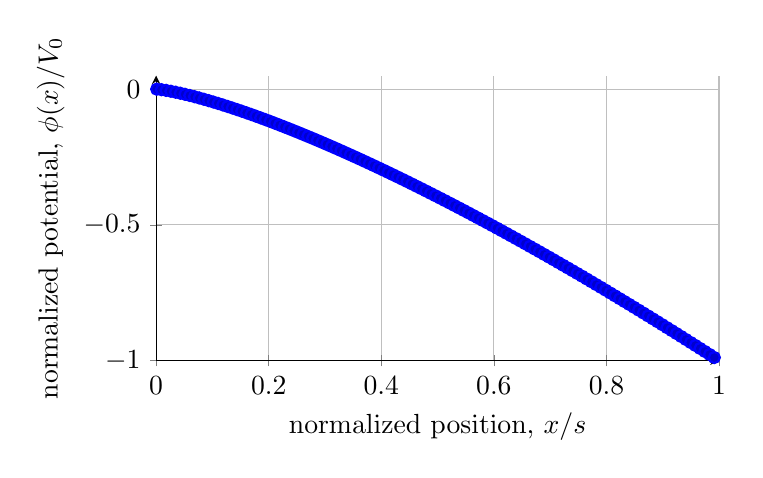
\begin{tikzpicture}
\begin{axis}[
 width=0.72\linewidth,
 height=5.2cm,
 xlabel={normalized position, $x/s$},
 ylabel={normalized potential, $\phi(x)/V_{0}$},
 domain=0.001:1,
 samples=120,
 grid=both,
 axis lines=left,
 xmin=0, xmax=1,
 ymin=-1, ymax=0.05,
 every axis plot/.append style={black, thick},
]
\addplot {-(x)^(4/3)};
\end{axis}
\end{tikzpicture}
\caption{Normalized Child--Langmuir sheath potential profile $\phi(x)/V_{0} = -(x/s)^{4/3}$ from the analytic solution of Eq.~\eqref{eq:cl-ode}, plotted from the sheath edge ($x/s=0$) to the wall ($x/s=1$); a direct evaluation of the closed-form expression, not measured or simulated data.}
\label{fig:child-langmuir-profile}
\end{figure}

\subsection{Regions of the plasma-boundary transition}

Figure~\ref{fig:sheath-regions} summarizes the full spatial structure of the plasma-wall transition: a quasineutral bulk plasma sourcing ions essentially at rest; a quasineutral presheath, extending over a scale much larger than $\lambda_{\mathrm{D}}$, across which the weak ambipolar field accelerates ions to $u_{\mathrm{B}}$ while $\phi$ falls by $T_{\mathrm{e}}/2e$; and the non-neutral sheath, extending only a few to a few tens of $\lambda_{\mathrm{D}}$, across which essentially the entire remaining drop $V_{0}$ occurs \cite{ref0013,ref0023}.

\begin{figure}[htbp]
\centering
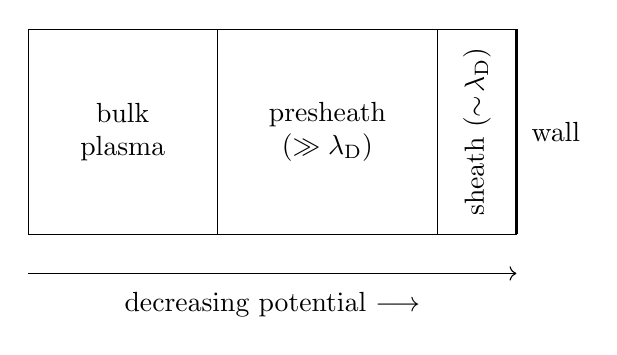
\begin{tikzpicture}[x=1cm, y=1cm]
\draw[black] (0,0) rectangle (2.4,2.6);
\draw[black] (2.4,0) rectangle (5.2,2.6);
\draw[black] (5.2,0) rectangle (6.2,2.6);
\draw[black, very thick] (6.2,0) -- (6.2,2.6);
\node[align=center] at (1.2,1.3) {bulk\\plasma};
\node[align=center] at (3.8,1.3) {presheath\\($\gg \lambda_{\mathrm{D}}$)};
\node[align=center, rotate=90] at (5.7,1.3) {sheath ($\sim\!\lambda_{\mathrm{D}}$)};
\node at (6.7,1.3) {wall};
\draw[black,->] (0,-0.5) -- (6.2,-0.5) node[midway, below=2pt]{};
\node at (3.1,-0.9) {decreasing potential $\longrightarrow$};
\end{tikzpicture}
\caption{Schematic (not to scale) plasma--presheath--sheath--wall spatial decomposition. The presheath spans a scale much larger than $\lambda_{\mathrm{D}}$; the sheath spans only a few to a few tens of $\lambda_{\mathrm{D}}$.}
\label{fig:sheath-regions}
\end{figure}

\subsection{Comparative scaling summary}

Table~\ref{tab:sheath-scaling} collects the scaling laws derived above and the collisional/magnetized generalizations below.

\begin{table}[htbp]
\centering
\caption{Sheath thickness and current scaling laws in the principal regimes discussed in this chapter. $s$: sheath thickness; $\lambda_{\mathrm{Ds}}$: sheath-edge Debye length; $V_{0}$: sheath voltage; $\ell_{\mathrm{i}}$: ion-neutral mean free path.}
\label{tab:sheath-scaling}
\begin{tabular}{lll}
\toprule
Regime & Thickness scaling & Governing relation \\
\midrule
Matrix sheath & $s \propto \lambda_{\mathrm{Ds}} (V_{0}/T_{\mathrm{e}})^{1/2}$ & Eq.~\eqref{eq:matrix-sheath} \\
Child--Langmuir sheath & $s \propto \lambda_{\mathrm{Ds}} (V_{0}/T_{\mathrm{e}})^{3/4}$ & Eq.~\eqref{eq:cl-thickness} \\
Collisional (mobility-limited) sheath & $s \propto \lambda_{\mathrm{Ds}}^{4/5} \ell_{\mathrm{i}}^{1/5} (V_{0}/T_{\mathrm{e}})^{2/5}$ & Section~\ref{sec:collisional} \\
Bohm--Chodura magnetic presheath & width $\sim \rho_{\mathrm{i}}$ (ion Larmor radius) & Section~\ref{sec:chodura} \\
\bottomrule
\end{tabular}
\end{table}

\section{Collisional Sheaths and the Bohm--Chodura Criterion}
\label{sec:collisional}

\subsection{Ion-neutral collisions in the presheath}

The derivation of Section~\ref{ch03-sec:bohm} assumed ions are collisionless across the presheath and sheath. In many technologically relevant plasmas -- moderate-pressure capacitively or inductively coupled discharges -- the ion-neutral mean free path $\ell_{\mathrm{i}}$ can be comparable to, or smaller than, the presheath length. Collisions drag on the ion fluid, requiring a larger presheath field to reach the sheath-edge criterion, and broaden $f_{\mathrm{i}}(v)$ at the sheath edge, since ions undergo their last collision at varying distances from the wall \cite{ref0009,ref0024}.

\subsection{The generalized collisional Bohm criterion}

A convenient generalization retains the fluid momentum equation but adds a friction term proportional to the ion-neutral collision frequency $\nu_{\mathrm{i}n}$:
\begin{equation}
m_{\mathrm{i}} n_{\mathrm{i}} u_{\mathrm{i}} \frac{\mathrm{d}u_{\mathrm{i}}}{\mathrm{d}x} = -e n_{\mathrm{i}} \frac{\mathrm{d}\phi}{\mathrm{d}x} - m_{\mathrm{i}} n_{\mathrm{i}} \nu_{\mathrm{i}n} u_{\mathrm{i}}.
\label{eq:collisional-momentum}
\end{equation}
Repeating the linear-stability argument of Section~\ref{ch03-sec:bohm} with Eq.~\eqref{eq:collisional-momentum} shows the marginal sheath-edge speed is modified from the simple $u_{\mathrm{B}}$ of Eq.~\eqref{ch03-eq:bohm-criterion}; in the constant-mean-free-path limit it becomes a function of $\lambda_{\mathrm{Ds}}/\ell_{\mathrm{i}}$, approaching $u_{\mathrm{B}}$ as $\lambda_{\mathrm{Ds}}/\ell_{\mathrm{i}} \to 0$ and falling somewhat below $u_{\mathrm{B}}$ as collisionality increases, since collisions supply part of the ``stiffening'' inertia alone provided in the collisionless case \cite{ref0009,ref0024,ref0015}. Two-fluid treatments retaining finite $T_{\mathrm{i}}$ show a warm-ion presheath both reduces the required sheath-edge velocity and modifies the density factor away from the cold-ion value $\exp(-1/2)$ \cite{ref0023}.

\subsection{Mobility-limited (high-pressure) sheath thickness}

In the opposite, strongly collisional limit, where the ion mean free path is much smaller than the sheath thickness, ion transport is dominated by mobility rather than free acceleration: $u_{\mathrm{i}} = \mu_{\mathrm{i}} E$. Repeating the Child--Langmuir derivation with this relation, the sheath thickness scales approximately as
\begin{equation}
s_{\mathrm{mob}} \propto \lambda_{\mathrm{Ds}}^{4/5}\, \ell_{\mathrm{i}}^{1/5} \left( \frac{e V_{0}}{k_{\mathrm{B}} T_{\mathrm{e}}} \right)^{2/5},
\end{equation}
a weaker voltage dependence than the collisionless $3/4$-power law, reflecting additional damping by collisions with the neutral background \cite{ref0024}. The resulting reduction of net ion flux to the wall as collisionality increases has direct consequences for $\Gamma_{E}$, treated as a correction factor in later chapters \cite{ref0024}.

\subsection{Magnetized presheath and the Chodura layer}
\label{sec:chodura}

When a static magnetic field $\mathbf{B}$ is present at the plasma boundary -- fusion divertors, magnetized processing plasmas, Hall-effect thrusters -- the presheath acquires structure not captured by unmagnetized theory. If $\mathbf{B}$ is oblique to the wall (angle $\alpha \ne 90^{\circ}$), ion gyromotion introduces a new intermediate scale, the ion Larmor radius $\rho_{\mathrm{i}} = m_{\mathrm{i}} v_{\perp}/(eB)$, with $\lambda_{\mathrm{D}} \ll \rho_{\mathrm{i}} \ll$ (collisional presheath scale). Chodura showed a new, quasineutral \emph{magnetic presheath} of width $\sim \rho_{\mathrm{i}}$ must be inserted between the traditional presheath and the electrostatic Debye sheath, within which ions accelerate along the field line while deflected by $\mathbf{E}\times\mathbf{B}$ and gyro-motion toward the wall \cite{ref0017,ref0018}.

\subsection{The Bohm--Chodura criterion}

Within this magnetic presheath, the generalized Bohm--Chodura criterion requires the ion drift component \emph{along the magnetic field}, $u_{\parallel}$, to reach the acoustic speed at the entrance to the magnetic presheath,
\begin{equation}
u_{\parallel} \ge u_{\mathrm{B}} = \sqrt{\frac{k_{\mathrm{B}} T_{\mathrm{e}}}{m_{\mathrm{i}}}},
\label{eq:chodura-parallel}
\end{equation}
while quasineutrality and the magnetic presheath geometry simultaneously require the ion velocity component \emph{normal to the wall}, $u_{\perp,\mathrm{wall}}$, to reach at least $u_{\mathrm{B}} \sin\alpha$ by the time ions reach the Debye-scale electrostatic sheath edge \cite{ref0017,ref0018}:
\begin{equation}
u_{\perp,\mathrm{wall}} \ge u_{\mathrm{B}} \sin\alpha.
\label{eq:chodura-normal}
\end{equation}
As $\alpha \to 90^{\circ}$, Eqs.~\eqref{eq:chodura-parallel} and~\eqref{eq:chodura-normal} coincide and the unmagnetized Bohm criterion is recovered; for grazing incidence ($\alpha \to 0$), the normal-velocity requirement weakens, since gyro-orbits carry ions only slowly toward the wall even though their parallel speed is already sonic \cite{ref0017,ref0018}. The magnetic presheath thus adds a fourth region, intermediate in scale ($\rho_{\mathrm{i}}$), to the spatial hierarchy of a magnetized, weakly collisional boundary plasma.

\section{Radio-Frequency and Capacitive Sheaths}

\subsection{Why time dependence matters}

The sheath theory developed so far is strictly a DC construction. Many technologically important plasmas are sustained or biased with radio-frequency (RF) power, from tens of kHz to hundreds of MHz, and the sheath adjacent to an RF-driven electrode oscillates in thickness and instantaneous voltage with the applied waveform. Whether ions respond quasi-statically, average over the oscillation, or respond in some intermediate fashion depends on the ratio of the ion transit time, $\tau_{\mathrm{i}} \sim s/u_{\mathrm{B}}$, to the RF period $\tau_{\mathrm{rf}} = 2\pi/\omega$.

\subsection{Frequency regimes}

In the \emph{low-frequency} regime, $\omega \tau_{\mathrm{i}} \ll 1$, ions cross the sheath in a small fraction of an RF cycle and respond essentially instantaneously: the sheath can be modelled at each instant by the DC matrix or Child--Langmuir relations, tracking $V(t) = V_{0} + V_{\mathrm{rf}} \sin(\omega t)$ \cite{ref0043}. In the opposite, \emph{high-frequency} regime, $\omega \tau_{\mathrm{i}} \gg 1$, ions need many RF periods to cross the sheath and respond only to the time-averaged field, so the sheath behaves as a nonlinear capacitor whose ion flux is frozen at its time-averaged Bohm value \cite{ref0043}. Most capacitively coupled sources -- typically driven at $\SI{13.56}{\mega\hertz}$ or higher -- operate near the high-frequency regime for heavy ions and the low-frequency or intermediate regime for light ions, so a single discharge can display different sheath dynamics for different ion masses simultaneously \cite{ref0038,ref0040}.

\subsection{The intermediate regime and sheath harmonics}

Neither limit is exact for $\omega \tau_{\mathrm{i}} \sim 1$, the \emph{intermediate} regime relevant to many practical frequencies and pressures. Kinetic and particle-in-cell simulations show the sheath develops significant harmonic content beyond the fundamental drive frequency, tied to the nonlinear, voltage-dependent impedance of the space-charge layer \cite{ref0040,ref0043}, underlying waveform-tailoring techniques that decouple control of ion flux from mean ion energy. Equivalent-circuit descriptions, representing the sheath as a voltage-dependent capacitor in series with a bulk plasma resistance and inductance, offer a compact framework for interpreting these dynamics without full kinetic simulation.

\subsection{Collisional and magnetized RF sheaths}

The collisional and magnetized generalizations of Section~\ref{sec:collisional} carry over, with added complexity, to the RF case. Collisional RF sheath models track the instantaneous balance between ion inertia, collisional drag, and the time-varying field, showing that increasing pressure both damps the sheath-oscillation amplitude and broadens the ion energy spread at the wall \cite{ref0043}. In magnetized RF discharges, interaction of the oscillating sheath field with ion and electron gyromotion introduces frequency-dependent modification of the Bohm--Chodura condition, while secondary electron emission from an RF-biased surface can substantially modify or disrupt the classical RF sheath structure at high emission yield, particularly for dielectric walls \cite{ref0038}.

\subsection{Self-bias, asymmetry, and battery effects}

An RF-driven electrode capacitively coupled to the plasma (unable to pass net DC current) must develop, in steady state, a DC self-bias such that time-averaged ion and electron currents balance -- analogous to the DC floating condition of Eq.~\eqref{eq:floating-potential} but for cycle-averaged fluxes. When the areas, capacitances, or waveforms of the two electrodes bounding an RF discharge are unequal -- the \emph{asymmetric} discharge -- the two sheaths do not carry equal time-averaged voltage, and a substantial DC self-bias develops across the smaller electrode, a sheath ``battery effect'' that adds directly to the sheath voltage seen by ions there, a handle for controlling mean ion bombardment energy independently of discharge power.

\subsection{Bimodal ion energy distributions}

The single most important consequence of RF sheath dynamics for this monograph is the modification it produces in the ion energy distribution function (IEDF) delivered to the wall, relative to the mono-energetic result of Eq.~\eqref{eq:ion-impact-energy}. In the low-frequency limit, ions respond to the full instantaneous voltage swing, and because they spend a disproportionate fraction of the cycle near the two turning points of $V(t)$ (where $\mathrm{d}V/\mathrm{d}t \to 0$), the IEDF develops two pronounced peaks -- a \emph{bimodal} distribution -- near $e(V_{0} - V_{\mathrm{rf}})$ and $e(V_{0}+V_{\mathrm{rf}})$ \cite{ref0055}. As driving frequency increases toward the high-frequency limit, ions can no longer follow the instantaneous field, the peaks narrow and merge, and the IEDF collapses toward a single peak centred on the time-averaged sheath voltage \cite{ref0055,ref0040}. This transition shows why a purely time-averaged treatment cannot predict the true ion energy flux delivered by an RF-driven boundary: the flux-weighted mean energy and second moment of $f_{\mathrm{i}}(v)$ depend on the entire waveform of $V(t)$ relative to $\tau_{\mathrm{i}}$, not merely its mean.

\section{Kinetic Corrections and Finite-Debye-Length Effects}

\subsection{Limits of the cold-ion fluid picture}

The derivation of Section~\ref{ch03-sec:bohm} idealized the ion population as a cold, mono-energetic fluid entering the sheath at a single speed $u_{0}$. Real ion populations, even collisionless, arrive at the sheath edge with a spread of velocities set by their birth location in the presheath, since an ion born at $x'$ and accelerated freely to $x=0$ carries a speed set by the potential drop between $x'$ and $0$. The correct kinetic description replaces $u_{0}$ with a full velocity distribution $f_{\mathrm{i}}(v)$ at the sheath edge, normalized so $n_{\mathrm{s}} = \int_{0}^{\infty} f_{\mathrm{i}}(v)\, \mathrm{d}v$, and the fluid Bohm criterion must be re-derived as a moment condition \cite{ref0006}.

\subsection{The kinetic (Harrison--Thompson) Bohm criterion}

Repeating the linearized-Poisson argument with the ion density expressed as a velocity-space integral over $f_{\mathrm{i}}(v)$, the marginal-stability condition generalizes to an inequality on the $v^{-2}$-weighted moment:
\begin{equation}
\boxed{\, \int_{0}^{\infty} \frac{f_{\mathrm{i}}(v)}{v^{2}}\, \mathrm{d}v \;\le\; \frac{n_{\mathrm{s}}\, m_{\mathrm{i}}}{k_{\mathrm{B}} T_{\mathrm{e}}} \,}.
\label{eq:kinetic-bohm}
\end{equation}
Equation~\eqref{eq:kinetic-bohm} is the kinetic form of the Bohm criterion, sometimes attributed to Harrison and Thompson \cite{ref0001}. It reduces to the fluid criterion of Eq.~\eqref{ch03-eq:bohm-criterion} for a mono-energetic distribution $f_{\mathrm{i}}(v) = n_{\mathrm{s}}\, \delta(v-u_{0})$, for which the integral evaluates to $n_{\mathrm{s}}/u_{0}^{2}$. For a distribution with any spread, the $v^{-2}$ weighting means the criterion is dominated by the \emph{slowest} ions present: a small slow population can violate it even when the bulk, and the flux-averaged mean speed, comfortably exceeds $u_{\mathrm{B}}$ -- motivating fully kinetic treatments of the presheath--sheath transition via the Vlasov equation \cite{ref0659}.

\subsection{The Tonks--Langmuir kinetic model}

The paradigmatic fully kinetic treatment of the presheath--sheath system is the Tonks--Langmuir model, in which ions are created by ionization of a cold background at a spatially varying rate and fall freely, without collisions, from their birth point onward. Because an ion at $x$ may have been born anywhere between the plasma centre and $x$, the model self-consistently generates a broad, non-mono-energetic $f_{\mathrm{i}}(v;x)$ at every point, and whether the kinetic Bohm criterion, Eq.~\eqref{eq:kinetic-bohm}, is satisfied \emph{as a consequence of} the free-fall ionization kinematics -- rather than imposed separately -- has long been debated. Extensions to non-Maxwellian electron populations show the electron energy distribution shape feeds directly into the ionization source term and hence into the resulting ion distribution, altering numerical prefactors while leaving the qualitative structure intact.

\subsection{Continuum-kinetic and Vlasov simulation approaches}

Because the presheath-to-sheath transition spans several orders of magnitude in length scale and involves a genuinely non-Maxwellian, evolving ion distribution, it is a natural target for direct numerical solution of the Vlasov (collisionless kinetic) equation, alone or coupled to a Boltzmann collision operator for finite collisionality \cite{ref0670}. Continuum-kinetic (grid-based) discretizations of the Vlasov--Poisson system resolve the sheath and presheath self-consistently, requiring velocity-space resolution fine enough to avoid spurious noise near the sharp, nearly singular ion distribution at the sheath edge; bi-species Vlasov--Poisson--Boltzmann formulations extend this to explicitly collisional sheaths.

\subsection{Kinetic effects in magnetized and grazing-angle geometries}

The magnetic presheath problem of Section~\ref{sec:chodura} is intrinsically kinetic at grazing field angles, because ion gyro-orbits carrying particles toward the wall have a radius $\rho_{\mathrm{i}}$ comparable to the presheath scale itself, so a fluid (guiding-centre) description becomes progressively less accurate as $\alpha \to 0$. Large-gyro-orbit kinetic models, retaining the full cyclotron trajectory, show the ion distribution delivered to the Debye sheath at grazing incidence departs substantially from the shifted-Maxwellian or mono-energetic pictures used in the fluid Bohm--Chodura derivation, a departure confirmed qualitatively by laser-induced-fluorescence measurements of the presheath ion velocity distribution.

\subsection{Finite Debye-length (finite $\lambda_{\mathrm{D}}/L$) effects}

Every result derived in Sections~\ref{ch03-sec:bohm} through the present section relies on the formal scale separation $\lambda_{\mathrm{D}} \ll L$, where $L$ is the presheath or system length scale; the sharp division into a quasineutral presheath and a non-neutral sheath is an asymptotic statement valid as $\lambda_{\mathrm{D}}/L \to 0$. For finite, non-negligible $\lambda_{\mathrm{D}}/L$ -- relevant to small discharges, low-density plasmas, or dust-grain and probe sheaths only modestly larger than $\lambda_{\mathrm{D}}$ -- quasineutrality is not exactly satisfied anywhere, presheath and sheath blend continuously without a sharp edge, and the Bohm criterion must be reformulated as an asymptotic matching statement rather than a boundary condition at a precise location \cite{ref0012}. Systematic treatments solving Eq.~\eqref{ch03-eq:poisson-full} show the practical threshold ion speed approaches $u_{\mathrm{B}}$ smoothly from above as $\lambda_{\mathrm{D}}/L \to 0$, with calculable finite-size corrections to the sheath-edge density and potential offset. Related considerations govern the electron-rich, or electron-sheath, regime near strongly electron-emitting or highly negatively charged boundaries, where the roles of light and heavy species reverse \cite{ref0006}.

\subsection{Practical implications for the fluid picture used elsewhere}

The kinetic and finite-Debye-length corrections surveyed here do not overturn the fluid framework of Sections~\ref{ch03-sec:bohm}--\ref{sec:collisional}; rather, they define its domain of validity. For the great majority of laboratory low-temperature plasmas relevant to ion energy flux measurement -- $\lambda_{\mathrm{D}}$ typically tens of micrometres to a few millimetres, system scales centimetres or more -- the fluid Bohm criterion and Child--Langmuir thickness scaling of Eq.~\eqref{eq:cl-thickness} remain quantitatively reliable and underlie the ion energy flux formalism developed in the following chapter. Kinetic corrections become essential in strongly grazing magnetic field angles, RF sheaths at low $\omega\tau_{\mathrm{i}}$ with broad IEDFs, multi-ion-species and electronegative plasmas, and any boundary not overwhelmingly larger than $\lambda_{\mathrm{D}}$.

\subsection{Consequences for the energy-flux moment}

Returning to Eq.~\eqref{eq:energy-flux-moments}, each correction surveyed here reshapes the second (energy-weighted) moment $\Gamma_{E}$ relative to the idealized delta-function prediction of Eq.~\eqref{eq:ion-impact-energy}. Ion-neutral collisions (Section~\ref{sec:collisional}) remove high-energy ions from the beam via charge exchange and momentum-transfer scattering while injecting slow, newly created ions, broadening $f_{\mathrm{i}}(v)$ at the wall toward lower energies and lowering $\Gamma_{E}$ relative to $\Gamma_{\mathrm{i}} E_{\mathrm{i}}$ \cite{ref0024}. The Bohm--Chodura magnetized criterion (Section~\ref{sec:chodura}) instead redistributes energy between wall-normal and wall-tangential velocity components: since only the normal component contributes to the flux crossing the Debye sheath while the full speed contributes to kinetic energy, oblique magnetic incidence generally reduces the normal-direction energy flux at fixed sheath voltage, more pronounced near grazing incidence \cite{ref0017,ref0018}. The RF sheaths of Section~6 modify $\Gamma_{E}$ differently again: the correct energy flux is a flux-weighted average over the periodic waveform, $\Gamma_{E} \propto \langle V(t)^{3/2} \rangle_{t}$ in the space-charge-limited regime, systematically larger than $\langle V(t) \rangle_{t}^{3/2}$ by the convexity of $V^{3/2}$ (Jensen's inequality) \cite{ref0055}. Finally, the kinetic corrections act principally on the low-velocity tail of $f_{\mathrm{i}}(v)$ and so have a comparatively modest direct effect on $\Gamma_{E}$ (dominated by the high-velocity tail), even though that same low-velocity tail controls the marginal Bohm criterion -- why sheath-edge diagnostics testing the Bohm criterion and wall-plane diagnostics quantifying $\Gamma_{E}$ probe weakly correlated features of the same distribution.

\section{Summary}

This chapter developed the theory of the plasma sheath from the elementary flux-balance argument for its existence through to its full kinetic and magnetized generalizations. The disparity between electron and ion thermal mobilities forces the formation of a non-neutral boundary layer that establishes current balance at any material surface; the resulting floating, wall, and plasma potentials are fixed by the exponential retardation of the electron flux against the comparatively rigid ion flux delivered by the Bohm criterion, $u_{0} \ge u_{\mathrm{B}} = \sqrt{k_{\mathrm{B}} T_{\mathrm{e}}/m_{\mathrm{i}}}$, derived from requiring the space-charge Poisson equation admit a monotonic solution. Its enforcement by a quasineutral presheath -- imposing a universal potential drop of $T_{\mathrm{e}}/2$ and a sheath-edge density reduction of $\exp(-1/2)$ in the cold-ion, collisionless limit -- accelerates thermal ions to the sheath entrance condition, and the sheath itself has a thickness of order a few Debye lengths in the matrix approximation, growing as $(V_{0}/T_{\mathrm{e}})^{3/4}$ in the self-consistent Child--Langmuir regime.

Collisions relax and reshape this picture toward a mobility-limited sheath at high pressure, while an oblique magnetic field imposes an entirely new intermediate structure, the Chodura magnetic presheath, governed by the joint Bohm--Chodura conditions on parallel and wall-normal ion velocity. Time-dependent RF excitation interpolates between a quasi-static, DC-like sheath at low frequency and a time-averaged, capacitor-like sheath at high frequency, with the intermediate regime responsible for the characteristic bimodal ion energy distributions at capacitively coupled discharge walls. Kinetic corrections -- most importantly the Harrison--Thompson generalization of the Bohm criterion to a $v^{-2}$-weighted moment of $f_{\mathrm{i}}(v)$ -- refine, and in several regimes (grazing magnetic incidence, low-frequency RF, finite $\lambda_{\mathrm{D}}/L$, multi-species and electronegative plasmas) qualitatively supersede, the cold-fluid picture.

In every regime treated here, the sheath converts a thermal, near-isotropic ion population in the plasma bulk into a directed, accelerated flux striking the wall with an energy set by the local sheath voltage (and, more generally, by the full time- and velocity-resolved history of that voltage as sampled by $f_{\mathrm{i}}(v)$). It is this conversion -- quantified through the particle flux $\Gamma_{\mathrm{i}} = n_{\mathrm{s}} u_{\mathrm{B}}$ and the mean ion impact energy of Eq.~\eqref{eq:ion-impact-energy}, or their collisional, magnetized, and RF-modulated generalizations -- that defines $\Gamma_{E}$ at the heart of this monograph, and forms the theoretical foundation for the sensor design and diagnostics developed in the chapters that follow.

\chapter{Ion Energy Flux: Definition and Physical Significance}
\label{ch:ief}

The preceding chapters established the plasma sheath as the thin, quasi-neutrality-violating boundary layer through which a bounded plasma communicates with a material surface. This chapter addresses the quantity this monograph takes as its principal diagnostic and design target: the \emph{ion energy flux}, $\Gamma_{E}$, the rate at which kinetic energy carried by ions is delivered per unit area to a plasma-facing surface. Where the particle flux $\Gamma_{\mathrm{i}}$ answers \emph{how many} ions arrive, $\Gamma_E$ answers \emph{how much energy} arrives with them, and this second question governs sputtering yield, etch rate, implantation depth, surface heating, and material damage across plasma-facing applications. We fix definitions and units for particle and energy flux, construct $\Gamma_{E}$ as a moment of the ion velocity distribution function $f_{\mathrm{i}}(v)$, decompose the mean ion energy into directed and thermal parts, describe the ion energy and velocity distribution functions (IEDF/IVDF) carrying this information at a bounding surface, place the ion channel within the full wall power balance, quantify the sensitivity of $\Gamma_{E}$ to $T_{\mathrm{e}}$, $n_{\mathrm{s}}$, and the sheath potential drop, and close by explaining why $\Gamma_{E}$ is not directly measurable -- motivating the reconstruction-based approach of the chapters that follow.

\section{Particle Flux and Energy Flux: Formal Definitions and Units}

\subsection{Particle flux at a bounding surface}

Consider a plasma-facing surface with outward unit normal $\hat{n}$, and let $f_{\mathrm{i}}(\vec r, \vec v, t)$ denote the ion phase-space distribution function, normalized so $n_{\mathrm{i}}(\vec r, t) = \int f_{\mathrm{i}}(\vec r, \vec v, t)\, \mathrm{d}^3 v$ is the local ion number density. The particle flux crossing a surface element is the first velocity moment of $f_{\mathrm{i}}$ projected onto $\hat n$,
\begin{equation}
\Gamma_{\mathrm{i}}(\vec r, t) \;\equiv\; \int_{\mathbb{R}^3} (\vec v \cdot \hat n)\, f_{\mathrm{i}}(\vec r, \vec v, t)\, \mathrm{d}^3 v \;=\; n_{\mathrm{i}}(\vec r,t)\, u_{\mathrm{i}}(\vec r,t),
\label{eq:Gamma-i-def}
\end{equation}
where $u_{\mathrm{i}} \equiv \langle \vec v \cdot \hat n \rangle$ is the mean ion drift speed normal to the surface. Equation~\eqref{eq:Gamma-i-def} has SI units $\si{\per\square\meter\per\second}$ and is the flux measured by a planar probe biased into ion saturation. At the wall, flux conservation through the collisionless sheath links the wall flux to the flux at the sheath edge, $\Gamma_{\mathrm{i}}(\text{wall}) \approx n_{\mathrm{s}} u_{\mathrm{B}}$, with $n_{\mathrm{s}}$ the sheath-edge density and $u_{\mathrm{B}} = \sqrt{T_{\mathrm{e}}/m_{\mathrm{i}}}$ the Bohm speed (temperatures in energy units, $T_{\mathrm{e}} \equiv k_{\mathrm B} T_{\mathrm{e}}$). This near-conservation makes $n_{\mathrm{s}}$, rather than the larger, less accessible wall-adjacent density, the natural anchor point for surface flux calculations -- a role revisited for non-Maxwellian bulk populations in \cite{ref0090}.

\subsection{Energy flux and its physical dimensions}

The energy flux weights each ion's contribution by its kinetic energy $\tfrac{1}{2} m_{\mathrm{i}} v^2$ rather than unity:
\begin{equation}
\Gamma_{E}(\vec r, t) \;\equiv\; \int_{\mathbb{R}^3} \left(\tfrac{1}{2} m_{\mathrm{i}} v^2\right) (\vec v \cdot \hat n)\, f_{\mathrm{i}}(\vec r, \vec v, t)\, \mathrm{d}^3 v.
\label{eq:GammaE-def}
\end{equation}
Dimensionally, $\Gamma_{E}$ is a power per unit area, $\si{\watt\per\square\meter}$, or $\si{\electronvolt\per\square\meter\per\second}$ ($\SI{1}{\electronvolt\per\square\meter\per\second} = \SI{1.602e-19}{\watt\per\square\meter}$). It must be distinguished from the total heat flux $q_{\mathrm{wall}}$, which sums the ion channel with electron, recombination, radiative and secondary-emission contributions (\cref{sec:power-balance}). $\Gamma_{E}$ drives sputtering, ion-assisted etching, and implantation dose-energy products, whereas $q_{\mathrm{wall}}$ governs thermal-management calculations; conflating the two is a common error, flagged in etch-profile modelling \cite{ref0074} and reactive-ion etching of wafers \cite{ref0080}.

\subsection{Distinguishing \texorpdfstring{$\Gamma_{E}$}{Gamma\_E} from related quantities}

Three quantities are frequently confused with $\Gamma_{E}$. First, the ion \emph{energy density} $w_{\mathrm{i}} = \int \tfrac12 m_{\mathrm{i}} v^2 f_{\mathrm{i}}\, \mathrm{d}^3 v$ is volumetric ($\si{\joule\per\cubic\meter}$), not a flux, until convected across a surface via the $(\vec v\cdot\hat n)$ weighting in \cref{eq:GammaE-def}. Second, the \emph{mean ion energy} $\langle E_{\mathrm{i}}\rangle \equiv \Gamma_{E}/\Gamma_{\mathrm{i}}$ is an energy, not a flux, and is what energy-resolved diagnostics such as retarding-field analyzers report directly; $\Gamma_{E}$ requires this multiplied by the co-located particle flux, a combination \cref{sec:observability} shows is rarely available from one measurement. Third, the sheath \emph{heat transmission coefficient} $\gamma_{\mathrm{i}}$, ubiquitous in fusion edge-plasma work \cite{ref0093}, is dimensionless, defined by $\Gamma_{E} \equiv \gamma_{\mathrm{i}} T_{\mathrm{e}} \Gamma_{\mathrm{i}}$; it packages the energetics of \cref{sec:contributions} into one factor, useful for quick estimates but obscuring the dependence on sheath potential made explicit here.

\subsection{Application domains that motivate precise knowledge of \texorpdfstring{$\Gamma_{E}$}{Gamma\_E}}

The stakes attached to an accurate $\Gamma_{E}$ vary across settings. In reactive-ion and plasma-immersion processing, the ion energy flux through a pulsed or biased sheath sets the achievable implantation dose-energy product and treated-layer depth profile. In magnetron physical vapor deposition, particularly its high-power-impulse variant, the angularly resolved ion flux and its energy content control film growth mode, stoichiometry, and microstructure, an effect exploited by the ultra-low-frequency electrical asymmetry effect to tailor the delivered ion energy distribution in biased inductively coupled configurations \cite{ref0106}. In electric propulsion, by contrast, the ion energy flux exhausted from a thruster's acceleration region is the primary quantity of interest, not a boundary condition to minimize, since it is proportional to the product of thrust and exhaust velocity (thrust $\times$ $I_{\mathrm{sp}} g_0$); diagnostics of a Hall-effect thruster plume \cite{ref0114} and reviews of ion thrusters maturing into a mainstream technology \cite{ref0115} underscore how the same quantity carries opposite engineering connotations -- suppressed at a wafer, maximized at a thruster exit. This diversity is why a general, first-principles formulation of $\Gamma_{E}$, rather than case-specific rules, is the right starting point for the reconstruction methodology built later.

\section{The Ion Energy Flux Integral over the Ion Velocity Distribution Function}

\subsection{Moments of \texorpdfstring{$f_{\mathrm{i}}(v)$}{f\_i(v)}: density, flux, and energy flux}

$\Gamma_{E}$ is the energy-weighted first velocity moment of $f_{\mathrm{i}}$, usefully placed within the full moment hierarchy any kinetic or fluid model of the sheath must resolve: the zeroth moment is the density $n_{\mathrm{i}} = \int f_{\mathrm{i}}\, \mathrm{d}^3 v$, the first is $\Gamma_{\mathrm{i}}$, the second yields pressure and kinetic energy density, and $\Gamma_{E}$, built from $v^2 \times v$, is formally a \emph{third}-order moment along $\hat n$. This matters practically: third-order moments are far more sensitive to the high-velocity tail of $f_{\mathrm{i}}$ than the density or flux, so details nearly invisible in $n_{\mathrm{i}}$ or $\Gamma_{\mathrm{i}}$ -- a modest high-energy shoulder from charge exchange or RF sheath modulation -- can dominate $\Gamma_{E}$. This is why fluid closures built only on density and momentum moments routinely fail to capture the ion energy spectrum, motivating fluid models carrying an explicit ion energy-spectrum equation \cite{ref0083} and kinetic treatments resolving the full IVDF at the sheath boundary as a boundary condition in its own right \cite{ref0119}.

For a general non-Maxwellian, drifting, multi-component ion population, no closed-form expression for $\Gamma_{E}$ exists without specifying $f_{\mathrm{i}}$; a useful reference case is the drifting Maxwellian, $f_{\mathrm{i}}(\vec v) = n_{\mathrm{i}} \left(m_{\mathrm{i}}/2\pi T_{\mathrm{i}}\right)^{3/2} \exp\!\left[-m_{\mathrm{i}}(\vec v - \vec u_{\mathrm{i}})^2/2T_{\mathrm{i}}\right]$, for which \cref{eq:GammaE-def} along the drift direction gives the standard fluid closure
\begin{equation}
\Gamma_{E} \;=\; n_{\mathrm{i}} u_{\mathrm{i}} \left(\frac{1}{2} m_{\mathrm{i}} u_{\mathrm{i}}^2 + \frac{5}{2} T_{\mathrm{i}}\right) \;=\; \Gamma_{\mathrm{i}} \left(\frac{1}{2} m_{\mathrm{i}} u_{\mathrm{i}}^2 + \frac{5}{2} T_{\mathrm{i}}\right).
\label{eq:GammaE-drifting-maxwellian}
\end{equation}
The coefficient $5/2$ (not the naive $3/2$) arises because the energy flux carries not only the convected thermal energy $\tfrac32 T_{\mathrm{i}}$ but also the $p\,\mathrm{d}V$ pressure-work term $n_{\mathrm{i}} T_{\mathrm{i}} u_{\mathrm{i}}$ -- an enthalpy-like flux rather than a purely kinetic one. \Cref{eq:GammaE-drifting-maxwellian} is a useful reference precisely because real sheath-edge IVDFs are \emph{not} drifting Maxwellians (truncated by the loss cone into the sheath, often with non-Gaussian tails), so deviations from it are themselves diagnostic of the shape of $f_{\mathrm{i}}$, developed further using non-Maxwellian sheath-formation criteria in \cite{ref0090}.

\subsection{Reduction to a one-dimensional surface-normal problem}

For a planar, unmagnetized (or weakly magnetized, field-aligned) sheath, transverse velocity components decouple from the acceleration along $\hat n$, and it is convenient to use the reduced one-dimensional IVDF,
\begin{equation}
f_{\mathrm{i}}(v_z) \;\equiv\; \int\!\!\int f_{\mathrm{i}}(v_x, v_y, v_z)\, \mathrm{d}v_x\, \mathrm{d}v_y,
\end{equation}
with $z$ along $\hat n$. The particle and energy fluxes at any plane $z$ then collapse to one-dimensional integrals over the outward-directed half of velocity space,
\begin{align}
\Gamma_{\mathrm{i}}(z) &= \int_0^{\infty} v_z\, f_{\mathrm{i}}(v_z)\, \mathrm{d}v_z, \label{eq:Gamma-i-1D}\\
\Gamma_{E}(z) &= \int_0^{\infty} \tfrac{1}{2} m_{\mathrm{i}} v_z^2 \cdot v_z\, f_{\mathrm{i}}(v_z)\, \mathrm{d}v_z. \label{eq:GammaE-1D}
\end{align}
This is the working form used throughout the sheath-diagnostics literature, since energy- and velocity-resolved instruments (retarding-field analyzers, laser-induced fluorescence, mass-resolved energy analyzers) are sensitive to the surface-normal velocity component and report, in effect, $f_{\mathrm{i}}(v_z)$ or its energy-space image.

\subsection{The energy flux in terms of the normalized ion energy distribution function}

It is often more transparent to work in energy space. Define the normalized ion energy distribution function (IEDF) $f_E(E)$ via $E = \tfrac12 m_{\mathrm{i}} v_z^2$, $\mathrm{d}E = m_{\mathrm{i}} v_z\, \mathrm{d}v_z$, such that
\begin{equation}
\int_0^{\infty} f_E(E)\, \mathrm{d}E = 1,
\end{equation}
i.e., $f_E(E)$ is a probability density over arriving-ion energy, independent of flux magnitude. With this normalization, \cref{eq:Gamma-i-1D,eq:GammaE-1D} combine into the compact, central relation
\begin{equation}
\boxed{\;\Gamma_{E} \;=\; \Gamma_{\mathrm{i}} \int_0^{\infty} E\, f_E(E)\, \mathrm{d}E \;=\; \Gamma_{\mathrm{i}}\, \langle E_{\mathrm{i}} \rangle\;}
\label{eq:GammaE-factorized}
\end{equation}
which states that $\Gamma_{E}$ factorizes into particle flux times mean ion energy from the shape-only IEDF. This is the single most important relation in this chapter: it separates \emph{how many} ions arrive, set by $n_{\mathrm{s}}$ and $u_{\mathrm{B}}$, from \emph{how energetic} each is, set by the shape of $f_E(E)$ -- the factorization \cref{sec:observability} shows is the root cause of $\Gamma_{E}$'s non-trivial observability.

\section{Contributions to the Ion Energy Flux: Directed Sheath-Gained Energy and Thermal Energy}
\label{sec:contributions}

\subsection{Ion history from bulk plasma to wall: presheath and sheath}

An ion born deep in the quasi-neutral bulk plasma has, on average, negligible directed energy; its energy at collection is acquired entirely during transit through the presheath and sheath. The presheath is the extended, weakly non-neutral region whose ambipolar field -- sustained by ions and electrons leaving the plasma at equal net rates -- accelerates ions from thermal speeds up to the Bohm speed $u_{\mathrm{B}} = \sqrt{T_{\mathrm{e}}/m_{\mathrm{i}}}$ by the sheath edge; the sheath proper is the much thinner, strongly non-neutral layer, typically several Debye lengths $\lambda_{\mathrm{D}} = \sqrt{\varepsilon_0 T_{\mathrm{e}}/n_{\mathrm{e}} e^2}$, across which most of the wall-directed potential drop occurs and ions are further accelerated essentially collisionlessly, or with partial energy randomization if collisional. Accounting for $\Gamma_{E}$ must therefore track \emph{both} the presheath and sheath potential drops.

\subsection{Decomposition of the mean ion energy}

Combining the presheath and sheath contributions, the mean kinetic energy of an ion arriving at the wall can be written, for a collisionless or weakly collisional sheath, as the sum of three terms:
\begin{equation}
\langle E_{\mathrm{i}} \rangle \;=\; \underbrace{\tfrac{1}{2} m_{\mathrm{i}} u_{\mathrm{B}}^2}_{\text{directed, presheath-acquired}} \;+\; \underbrace{e\,|\Delta\phi_{\mathrm{sh}}|}_{\text{directed, sheath-acquired}} \;+\; \underbrace{\alpha\, T_{\mathrm{i}}}_{\text{thermal spread}},
\label{eq:Ei-decomp}
\end{equation}
where $\Delta\phi_{\mathrm{sh}}$ is the potential drop across the sheath proper, and $\alpha$ is an order-unity factor ($1/2$--$5/2$ depending on the sheath-edge IVDF shape, cf.\ the $5/2\,T_{\mathrm{i}}$ coefficient of \cref{eq:GammaE-drifting-maxwellian}) capturing residual thermal broadening. Since $\tfrac12 m_{\mathrm{i}} u_{\mathrm{B}}^2 = \tfrac12 T_{\mathrm{e}}$, \cref{eq:Ei-decomp} becomes
\begin{equation}
\langle E_{\mathrm{i}} \rangle \;\approx\; \tfrac{1}{2} T_{\mathrm{e}} \;+\; e\,|\Delta\phi_{\mathrm{sh}}| \;+\; \alpha\, T_{\mathrm{i}}.
\label{eq:Ei-decomp-Te}
\end{equation}
For a floating, unbiased wall in a low-temperature electropositive discharge, $|\Delta\phi_{\mathrm{sh}}|$ is of order a few $T_{\mathrm{e}}/e$ (set by the zero-net-current condition); the presheath and sheath contributions are then comparable, and the thermal term is a modest correction for cold ions ($T_{\mathrm{i}} \ll T_{\mathrm{e}}$). For a deliberately or self-consistently biased wall -- DC-biased, RF self-biased, or under active ion-beam/plasma-immersion processing -- $|\Delta\phi_{\mathrm{sh}}|$ can reach tens to hundreds of volts, dwarfing $T_{\mathrm{e}}$, so \cref{eq:Ei-decomp-Te} reduces to $\langle E_{\mathrm{i}}\rangle \approx e|\Delta\phi_{\mathrm{sh}}|$. \Cref{fig:Ei-vs-V} renders this decomposition schematically.

\begin{figure}[htbp]
\centering
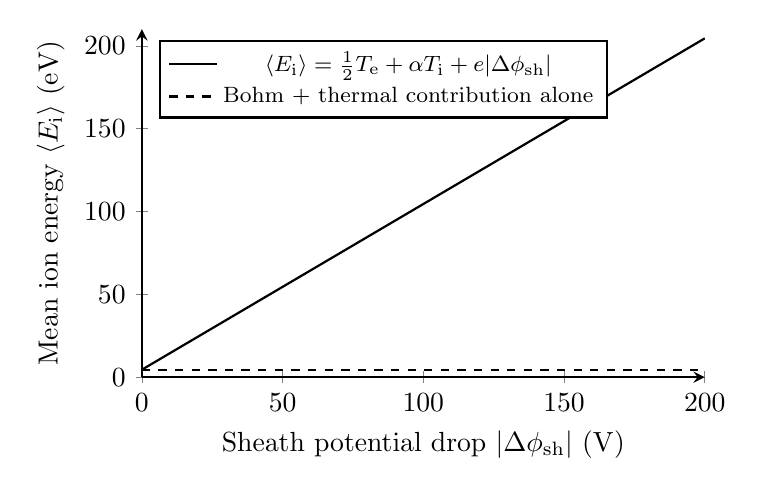
\begin{tikzpicture}
\begin{axis}[
 width=0.72\textwidth,
 height=6cm,
 xlabel={Sheath potential drop $|\Delta\phi_{\mathrm{sh}}|$ (\si{\volt})},
 ylabel={Mean ion energy $\langle E_{\mathrm{i}}\rangle$ (\si{\electronvolt})},
 xmin=0, xmax=200,
 ymin=0, ymax=210,
 domain=0:200,
 samples=50,
 axis lines=left,
 thick,
 legend style={draw=black, fill=white, font=\footnotesize, at={(0.03,0.97)}, anchor=north west},
]
\addplot[black, thick] {4.5 + x};
\addlegendentry{$\langle E_{\mathrm i}\rangle = \tfrac12 T_{\mathrm e} + \alpha T_{\mathrm i} + e|\Delta\phi_{\mathrm{sh}}|$}
\addplot[black, dashed] {4.5 + 0*x};
\addlegendentry{Bohm + thermal contribution alone}
\end{axis}
\end{tikzpicture}
\caption{Schematic, analytic illustration of \cref{eq:Ei-decomp-Te}: the mean ion energy delivered to the wall as a function of the sheath potential drop, evaluated for illustrative parameters $T_{\mathrm{e}} = \SI{3}{\electronvolt}$, $\alpha T_{\mathrm i} = \SI{3}{\electronvolt}$ (solid line), compared with the potential-independent presheath-plus-thermal contribution alone (dashed line). This is a plotted analytic function chosen to convey the linear scaling with sheath voltage, not measured or simulated data.}
\label{fig:Ei-vs-V}
\end{figure}

\subsection{The role of collisions in redistributing directed and thermal energy}

The decomposition of \cref{eq:Ei-decomp} assumes an effectively collisionless presheath and sheath, an assumption that fails once the ion-neutral mean free path becomes comparable to, or shorter than, these length scales. Charge-exchange and elastic collisions reduce the net ion flux reaching the wall by scattering ions out of the acceleration trajectory or generating slow ions locally within the sheath \cite{ref0077}, and reshape the energy distribution, converting directed sheath-gained energy into randomized thermal energy and populating a low-energy tail absent in the collisionless limit. In the strongly collisional regime relevant to plasma immersion ion implantation at moderate pressure, the delivered ion energy distribution becomes a convolution of the applied sheath voltage waveform with a collisional broadening kernel that shapes the resulting implantation-depth profile. Such effects act as corrections to, or generalizations of, the three-term decomposition of \cref{eq:Ei-decomp}, entering $\Gamma_{E}$ multiplicatively through \cref{eq:GammaE-factorized} via their effect on the shape of $f_E(E)$.

\subsection{Multiple ion species and the ion energy flux}

Real discharges frequently contain more than one ion species -- different charge states, chemically distinct positive ions, or coexisting positive and negative ions -- and the total ion energy flux is a sum over species,
\begin{equation}
\Gamma_{E}^{\mathrm{tot}} \;=\; \sum_{k} \Gamma_{E,k} \;=\; \sum_{k} \Gamma_{\mathrm{i},k} \langle E_{\mathrm{i},k} \rangle,
\end{equation}
where each species $k$ may reach the sheath edge with a different effective Bohm speed (lighter species can satisfy the generalized multi-species Bohm criterion at a lower fraction of their own Bohm speed) and so contribute disproportionately to $\Gamma_{E}^{\mathrm{tot}}$ relative to its number-density fraction, relevant to multi-species magnetized-sheath energy partitioning in processing tools with mixed feed gases \cite{ref0088}. The single-species framework of \cref{eq:Ei-decomp,eq:GammaE-factorized} generalizes directly, but the total energy flux can differ substantially from a single-species estimate using bulk plasma parameters alone.

\section{Ion Energy and Velocity Distribution Functions at Plasma-Bounded Surfaces}

\subsection{From \texorpdfstring{$f_{\mathrm{i}}(v)$}{f\_i(v)} to the IEDF}

The IVDF $f_{\mathrm{i}}(v)$ and the IEDF $f_E(E)$ are two representations of the same information, related by $E = \tfrac12 m_{\mathrm{i}} v^2$ and its Jacobian, $f_E(E)\, \mathrm{d}E = f_{\mathrm{i}}(v)\, \mathrm{d}v$ with $\mathrm{d}E = m_{\mathrm{i}} v\, \mathrm{d}v$. The IVDF is the more fundamental object kinetically -- it appears natively in the Vlasov equation governing ion evolution through the sheath -- while the IEDF is the representation most directly probed by energy-selective instruments and the one in which \cref{eq:GammaE-factorized} is most transparent. Both are used interchangeably: the IVDF matters whenever directional or angular information is needed (obliquely magnetized sheaths, off-normal incidence), while the IEDF is the natural currency for surface-process modelling, since sputtering yields, reaction probabilities, and implantation ranges are, to leading order, functions of the ion's kinetic energy at impact rather than its full velocity vector.

\subsection{Characteristic shapes of the IEDF: collisionless, RF-modulated, and collisionally broadened}

The shape of $f_E(E)$ at a surface depends strongly on the discharge regime; three archetypes recur. In a collisionless, DC or quasi-DC sheath, ions entering with the narrow, Bohm-speed-centered presheath distribution are accelerated by an essentially fixed potential, producing a relatively narrow IEDF tracking the presheath-plus-sheath energy of \cref{eq:Ei-decomp}, with spread set primarily by $T_{\mathrm{i}}$ and finite transit-time averaging, as targeted by dedicated ion-energy-flux sensors for plasma processing \cite{ref0075}. In an RF-driven sheath, the instantaneous sheath voltage oscillates at the driving frequency and its harmonics, so an ion transiting the sheath samples a time-varying potential; if transit time is short compared to the RF period, an ion "freezes in" a nearly instantaneous sheath voltage, and ions launched at different RF phases arrive with different energies, producing the celebrated \emph{bimodal} (or multi-peaked, at intermediate frequencies) IEDF bracketing the time-averaged sheath voltage; models spanning the full frequency range are developed in \cite{ref0123}. \Cref{fig:iedf-bimodal} sketches this bimodal shape.

\begin{figure}[htbp]
\centering
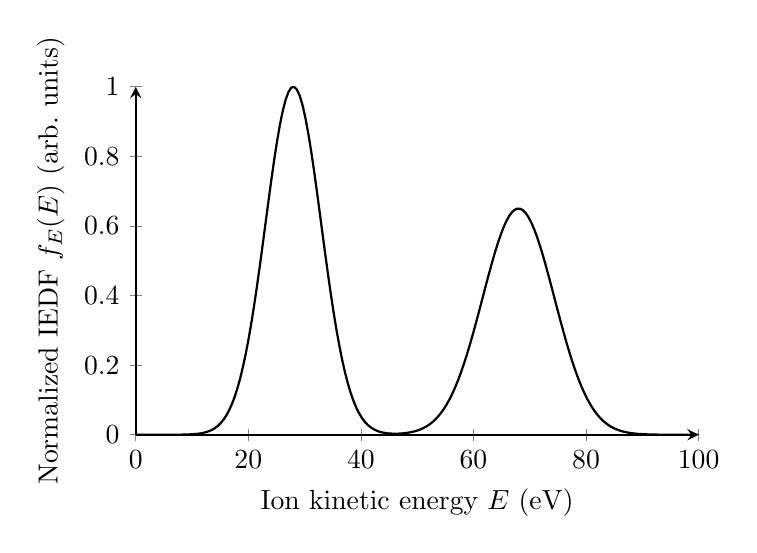
\begin{tikzpicture}
\begin{axis}[
 width=0.72\textwidth,
 height=6cm,
 xlabel={Ion kinetic energy $E$ (\si{\electronvolt})},
 ylabel={Normalized IEDF $f_E(E)$ (arb.\ units)},
 xmin=0, xmax=100,
 ymin=0,
 domain=0:100,
 samples=200,
 axis lines=left,
 thick,
]
\addplot[black, thick] {exp(-((x-28)/7)^2) + 0.65*exp(-((x-68)/9)^2)};
\end{axis}
\end{tikzpicture}
\caption{Schematic, illustrative bimodal ion energy distribution function of the type produced by radio-frequency modulation of the sheath potential drop, drawn as an explicit analytic superposition of two Gaussian components. The curve is not derived from measured or simulated data; it is intended only to convey the characteristic low- and high-energy peak structure discussed in the text.}
\label{fig:iedf-bimodal}
\end{figure}

\subsection{Angular structure, magnetization, and surface-emitted contributions}

Beyond the energy-space shape, the IVDF at a surface retains angular structure relevant to directional sputtering and shadowing in patterned geometries: even in a nominally normal-incidence planar sheath, thermal spread in transverse velocity combined with acceleration only along $\hat n$ narrows the angular spread of incidence as sheath potential increases (larger $e|\Delta\phi_{\mathrm{sh}}|$ collimates the beam), while magnetized sheaths and structured topography broaden it. It is also important to distinguish the IEDF of positive ions launched toward the surface -- this chapter's concern -- from the energy-and-angle distribution of particles \emph{emitted} back into the plasma (sputtered neutrals, backscattered ions, surface-generated negative ions); both matter physically but enter the wall power balance with opposite sign. Further complexity arises in dust-charged discharges or heavy-ion cathode-sheath environments, where the IEDF is shaped jointly by the sheath field and resonant charge-exchange collisions with heavier neutrals.

\subsection{Diagnostic access to the IEDF as a distribution, not merely its mean}

For most surface-process purposes it is not $\langle E_{\mathrm{i}}\rangle$ alone but the full shape of $f_E(E)$ that matters, because sputtering yield and reaction-probability curves are typically nonlinear (threshold-like at low energy, saturating at high energy), so the energy-flux-weighted average of a nonlinear yield function over $f_E(E)$ can differ substantially from the yield evaluated at $\langle E_{\mathrm{i}}\rangle$ alone. This motivates the broader program of "tailoring" the IEDF at plasma electrodes -- shaping the applied waveform to sculpt a desired energy distribution for process optimization -- surveyed comprehensively in \cite{ref0105}.

\section{Power Balance at the Wall: Ion, Electron, Recombination and Radiative Channels}
\label{sec:power-balance}

\subsection{The total power flux to a plasma-facing surface}

$\Gamma_{E}$ is one contribution -- often dominant for processing-relevant ion energies, but never the only one -- to the total power flux $q_{\mathrm{wall}}$ deposited on, or extracted from, a plasma-facing surface:
\begin{equation}
q_{\mathrm{wall}} \;=\; \Gamma_{E,\mathrm{ion}} \;+\; \Gamma_{E,\mathrm{electron}} \;+\; \Gamma_{\mathrm{i}}\, \varepsilon_{\mathrm{recomb}} \;-\; \Gamma_{\mathrm{see}}\, E_{\mathrm{see}} \;+\; q_{\mathrm{rad}},
\label{eq:power-balance-total}
\end{equation}
where the five terms are, respectively, the ion kinetic-plus-potential channel of this chapter, the electron thermal-flux channel, the energy released when an arriving ion recombines at the wall (recovering ionization energy $\varepsilon_{\mathrm{recomb}}$ as heat), the energy carried \emph{away} by secondary/backscattered electrons emitted with characteristic energy $E_{\mathrm{see}}$ at rate $\Gamma_{\mathrm{see}}$ (a loss term), and any net radiative flux $q_{\mathrm{rad}}$. Rigorous reactor-scale accounting of this balance, with ion and electron channels expressed through heat-transmission coefficients coupled to the confined-plasma energy balance, is treated in \cite{ref0093}, while device-specific total heat-flux measurements from ion bombardment of a wafer in an inductively coupled etch tool illustrate the practical side \cite{ref0080}. \Cref{tab:power-channels} summarizes the five channels.

\begin{table}[htbp]
\centering
\caption{Principal channels contributing to the total power flux deposited on a plasma-facing surface, \cref{eq:power-balance-total}. The ion energy flux $\Gamma_{E}$ that is the subject of this chapter constitutes only the first row; the remaining channels must be independently characterized, or subtracted, to isolate it from a total heat-load measurement.}
\label{tab:power-channels}
\begin{tabular}{@{}p{3.4cm}p{6.0cm}p{4.4cm}@{}}
\toprule
Channel & Physical origin & Sign / scaling \\
\midrule
Ion kinetic + potential ($\Gamma_{E,\mathrm{ion}}$) & Presheath (Bohm) and sheath acceleration plus thermal spread, \cref{eq:Ei-decomp-Te} & $+$; $\propto n_{\mathrm{s}} u_{\mathrm{B}}\, e|\Delta\phi_{\mathrm{sh}}|$ \\
Electron thermal ($\Gamma_{E,\mathrm{electron}}$) & High-energy tail of the (truncated) electron distribution reaching the wall & $+$; $\propto n_{\mathrm{s}} \bar v_{\mathrm{e}} T_{\mathrm{e}}$ \\
Recombination & Ionization energy released on neutralization at the surface & $+$; $\propto \Gamma_{\mathrm{i}}\,\varepsilon_{\mathrm{recomb}}$ \\
Secondary/backscattered emission & Energy carried away by electrons or ions ejected from the surface & $-$; $\propto \Gamma_{\mathrm{i}}\, \gamma_{\mathrm{se}}\, E_{\mathrm{see}}$ \\
Radiative & Photon absorption/emission at or near the surface & $\pm$; typically subdominant at low pressure, potentially significant in dense or strongly radiating plasmas \\
\bottomrule
\end{tabular}
\end{table}

\subsection{The ion channel and the sheath heat transmission coefficient}

Formally, the ion channel of \cref{eq:power-balance-total} is exactly $\Gamma_{E}$ as constructed in \cref{sec:contributions,eq:GammaE-factorized}, commonly packaged as $\Gamma_{E,\mathrm{ion}} = \gamma_{\mathrm{i}} T_{\mathrm{e}} \Gamma_{\mathrm{i}}$, defining $\gamma_{\mathrm{i}} \equiv \langle E_{\mathrm{i}}\rangle / T_{\mathrm{e}}$. For a floating wall with negligible bias, $\gamma_{\mathrm{i}}$ typically falls in the range $2$--$3$, reflecting \cref{eq:Ei-decomp-Te} at the floating potential; for actively biased surfaces, $\gamma_{\mathrm{i}}$ scales linearly with bias voltage over $T_{\mathrm{e}}$, so $\gamma_{\mathrm{i}} \gg 1$ is routine with substantial substrate bias. Data-driven approaches discovering closed-form heat-flux closures directly from kinetic or particle-in-cell simulation data offer an independent cross-check on closures of this kind \cite{ref0101}.

\subsection{The electron channel}

Electrons reaching the wall are drawn from the high-energy tail of the electron distribution with sufficient normal velocity to overcome the retarding sheath potential; for a floating or negatively biased wall this is an exponentially suppressed fraction of the bulk population, but because the electron thermal speed $\bar v_{\mathrm{e}} = \sqrt{8T_{\mathrm{e}}/\pi m_{\mathrm{e}}}$ is roughly $\sqrt{m_{\mathrm{i}}/m_{\mathrm{e}}}$ times the ion Bohm speed, the electron channel remains a significant, and for near-floating walls comparable, contributor to $q_{\mathrm{wall}}$. The electron and ion channels are not independent: ambipolarity directly determines $\Delta\phi_{\mathrm{sh}}$ in \cref{eq:Ei-decomp-Te}, so any change in the electron energy distribution alters the electron channel directly and the ion channel indirectly through the self-consistent sheath voltage.

\subsection{Recombination and secondary-emission channels}

The recombination channel is often neglected in low-temperature processing-plasma power balances since the ionization energy of common process gases is comparable to, or smaller than, typical sheath-acquired ion energies at moderate bias; it becomes non-negligible in high-density or high-charge-state plasmas and is retained in comprehensive reactor-scale balances \cite{ref0093}. The secondary-emission channel is more consequential: ion-induced (and, for energetic populations, electron-induced) secondary electron emission removes energy from the surface at a rate proportional to the incident flux and the secondary emission yield $\gamma_{\mathrm{se}}$, and because emitted secondaries are accelerated back out through the sheath potential, monitoring their energy and flux provides an indirect but accessible proxy for the incident ion flux, exploited in plasma-immersion implantation diagnostics tracking sheath-accelerated secondary electrons \cite{ref0078}.

\section{Sensitivity of the Ion Energy Flux to \texorpdfstring{$T_{\mathrm{e}}$}{Te}, \texorpdfstring{$n_{\mathrm{s}}$}{ns}, and Sheath Potential}

\subsection{Functional form and scaling}

Combining \cref{eq:GammaE-factorized} with the flux and mean-energy expressions of \cref{sec:contributions} gives an explicit functional form for $\Gamma_{E}$ in terms of the three controlling parameters emphasized throughout this monograph:
\begin{equation}
\Gamma_{E} \;=\; n_{\mathrm{s}} \sqrt{\frac{T_{\mathrm{e}}}{m_{\mathrm{i}}}} \left(\tfrac{1}{2} T_{\mathrm{e}} + e|\Delta\phi_{\mathrm{sh}}| + \alpha T_{\mathrm{i}}\right).
\label{eq:GammaE-scaling}
\end{equation}
Three structural features deserve emphasis. First, $\Gamma_{E}$ is exactly linear in $n_{\mathrm{s}}$, entering only through the flux prefactor -- a direct, testable consequence of \cref{eq:GammaE-factorized}. Second, $T_{\mathrm{e}}$ enters twice -- through the Bohm-speed prefactor $\sqrt{T_{\mathrm{e}}/m_{\mathrm{i}}}$ and the $\tfrac12 T_{\mathrm{e}}$ presheath-energy term -- so even at fixed sheath potential, $\Gamma_{E}$ is more sensitive to $T_{\mathrm{e}}$ than to $n_{\mathrm{s}}$ whenever the presheath term is not negligible compared with $e|\Delta\phi_{\mathrm{sh}}|$. Third, $\Delta\phi_{\mathrm{sh}}$ enters only inside the energy bracket, linearly, but is frequently not independent: at a floating wall it is set by $T_{\mathrm{e}}$ through ambipolarity, while at a biased wall it may be set externally or self-consistently by discharge power, geometry, and frequency.

\subsection{Logarithmic sensitivity coefficients}

It is convenient to express the sensitivity of $\Gamma_{E}$ to each parameter $X \in \{n_{\mathrm{s}}, T_{\mathrm{e}}, |\Delta\phi_{\mathrm{sh}}|\}$ through the logarithmic derivative $\partial \ln \Gamma_{E} / \partial \ln X$, useful for propagating measurement uncertainties. From \cref{eq:GammaE-scaling}, holding the other two parameters fixed,
\begin{align}
\frac{\partial \ln \Gamma_{E}}{\partial \ln n_{\mathrm{s}}} &= 1, \label{eq:sens-ns}\\[4pt]
\frac{\partial \ln \Gamma_{E}}{\partial \ln |\Delta\phi_{\mathrm{sh}}|} &= \frac{e|\Delta\phi_{\mathrm{sh}}|}{\tfrac12 T_{\mathrm{e}} + e|\Delta\phi_{\mathrm{sh}}| + \alpha T_{\mathrm{i}}}, \label{eq:sens-V}\\[4pt]
\frac{\partial \ln \Gamma_{E}}{\partial \ln T_{\mathrm{e}}} &= \frac{1}{2} + \frac{\tfrac12 T_{\mathrm{e}}}{\tfrac12 T_{\mathrm{e}} + e|\Delta\phi_{\mathrm{sh}}| + \alpha T_{\mathrm{i}}}, \label{eq:sens-Te}
\end{align}
where \cref{eq:sens-ns} is exact for all regimes, while \cref{eq:sens-V,eq:sens-Te} interpolate depending on the relative size of $e|\Delta\phi_{\mathrm{sh}}|$ and $T_{\mathrm{e}}$. In the strongly biased limit ($e|\Delta\phi_{\mathrm{sh}}| \gg T_{\mathrm{e}}$), \cref{eq:sens-V} tends to unity and \cref{eq:sens-Te} to $1/2$: $\Gamma_{E}$ scales linearly with bias voltage and as $\sqrt{T_{\mathrm{e}}}$ once the sheath energy term dominates. In the near-floating limit ($e|\Delta\phi_{\mathrm{sh}}| \sim T_{\mathrm{e}}$, with $\Delta\phi_{\mathrm{sh}} \propto T_{\mathrm{e}}$ through ambipolarity), the two contributions to $T_{\mathrm{e}}$-sensitivity add and the effective exponent rises toward $3/2$, so $\Gamma_{E}$ at a floating or lightly biased wall is considerably more sensitive to electron-temperature uncertainty than the naive $1/2$-power Bohm-flux scaling suggests. Non-Maxwellian electron populations reshape these Maxwellian-derived exponents.

\subsection{Regime dependence: floating, strongly biased, and RF self-biased walls}

\Cref{tab:sensitivity} collects illustrative sensitivity exponents for three representative regimes, from the limiting forms of \cref{eq:sens-ns,eq:sens-V,eq:sens-Te}. The magnetized-sheath case adds a further layer of sensitivity beyond \cref{eq:GammaE-scaling}, since the effective ion acceleration and delivered kinetic energy also depend on magnetic-field strength and obliquity \cite{ref0088}. A further important regime is a plasma at floating potential on a topographically or electrically patterned surface, where the local sheath structure -- and hence local $\Delta\phi_{\mathrm{sh}}$ and $\Gamma_{E}$ -- can vary substantially across the surface even with uniform bulk $n_{\mathrm{s}}$ and $T_{\mathrm{e}}$, a reminder that this sensitivity analysis strictly applies only locally.

\begin{table}[htbp]
\centering
\caption{Illustrative logarithmic sensitivity exponents $\partial \ln \Gamma_{E} / \partial \ln X$ of the ion energy flux to the sheath-edge density, electron temperature, and sheath potential drop, in three representative bias regimes, derived from the limiting forms of \cref{eq:sens-ns,eq:sens-V,eq:sens-Te}. The tabulated values are schematic, illustrating the analytic scaling rather than fitted results from measured or simulated discharges.}
\label{tab:sensitivity}
\begin{tabular}{@{}lccc@{}}
\toprule
Regime & $n_{\mathrm{s}}$ & $T_{\mathrm{e}}$ & $|\Delta\phi_{\mathrm{sh}}|$ \\
\midrule
Floating wall ($e|\Delta\phi_{\mathrm{sh}}| \propto T_{\mathrm{e}}$) & $1$ & $\approx 3/2$ & not independent of $T_{\mathrm{e}}$ \\
Strongly biased wall ($e|\Delta\phi_{\mathrm{sh}}| \gg T_{\mathrm{e}}$, external bias) & $1$ & $\approx 1/2$ & $\approx 1$ \\
RF self-bias (moderate collisionality) & $1$ & $1/2$--$1$ & $\approx 1$ \\
\bottomrule
\end{tabular}
\end{table}

\subsection{Propagation of measurement uncertainty into \texorpdfstring{$\Gamma_{E}$}{Gamma\_E}}

The sensitivity coefficients above propagate independent measurement uncertainties in $n_{\mathrm{s}}$, $T_{\mathrm{e}}$, and $\Delta\phi_{\mathrm{sh}}$ into an uncertainty estimate on the reconstructed $\Gamma_{E}$. Treating the three as uncorrelated, the fractional uncertainty follows the standard first-order propagation formula
\begin{equation}
\left(\frac{\delta \Gamma_{E}}{\Gamma_{E}}\right)^2 \;\approx\; \left(\frac{\partial \ln \Gamma_{E}}{\partial \ln n_{\mathrm{s}}}\right)^{2} \left(\frac{\delta n_{\mathrm{s}}}{n_{\mathrm{s}}}\right)^{2} + \left(\frac{\partial \ln \Gamma_{E}}{\partial \ln T_{\mathrm{e}}}\right)^{2} \left(\frac{\delta T_{\mathrm{e}}}{T_{\mathrm{e}}}\right)^{2} + \left(\frac{\partial \ln \Gamma_{E}}{\partial \ln |\Delta\phi_{\mathrm{sh}}|}\right)^{2} \left(\frac{\delta |\Delta\phi_{\mathrm{sh}}|}{|\Delta\phi_{\mathrm{sh}}|}\right)^{2}.
\label{ch04-eq:error-propagation}
\end{equation}
Because the exponents are all of order unity across every regime in \cref{tab:sensitivity}, \cref{ch04-eq:error-propagation} shows a fractional uncertainty on any one input parameter propagates into $\Gamma_{E}$ with roughly comparable, not strongly amplified or suppressed, weight. This is reassuring but not trivial: the dominant source of uncertainty in any practical reconstruction is the accuracy of the underlying diagnostics for $n_{\mathrm{s}}$, $T_{\mathrm{e}}$, and $\Delta\phi_{\mathrm{sh}}$ individually, not any intrinsic amplification in the combining expression. In practice, the electron-temperature term is usually the largest contributor to $\delta \Gamma_{E}/\Gamma_{E}$, both because $T_{\mathrm{e}}$ is often the least precisely determined of the three (nonlinear diagnostic inference, sensitivity to non-Maxwellian departures) and because its sensitivity exponent is largest near the floating-wall limit -- motivating the emphasis, in later diagnostic chapters, on obtaining $T_{\mathrm{e}}$ from methods insensitive to assumptions about the electron energy distribution function's shape.

\section{Why the Ion Energy Flux Is Not Directly Measurable}
\label{sec:observability}

\subsection{The instrumental gap between flux and energy}

The factorization $\Gamma_{E} = \Gamma_{\mathrm{i}} \langle E_{\mathrm{i}}\rangle$ is not merely a mathematical convenience; it exposes the central practical obstacle to measuring $\Gamma_{E}$ directly. Instruments that measure particle flux with high fidelity -- planar Langmuir probes in ion saturation, ion-collecting Faraday cups -- are, by design, energy-blind: they count ions regardless of individual kinetic energy, so their output is proportional to $\Gamma_{\mathrm{i}}$ alone. Conversely, instruments that resolve ion energy with high fidelity -- retarding-field analyzers, electrostatic/magnetic energy analyzers, velocity-resolved optics -- report the \emph{shape} of $f_E(E)$ but, in almost every practical implementation, only up to a poorly calibrated absolute normalization: grid transmission factors, finite acceptance angles, space-charge effects, and sheath perturbation by the analyzer's own biased aperture corrupt the absolute count rate while leaving the relative energy distribution comparatively unaffected. No single, standard instrument returns the product $\Gamma_{E} = \Gamma_{\mathrm{i}} \langle E_{\mathrm{i}} \rangle$ directly; $\Gamma_{E}$ must be reconstructed by combining an absolutely calibrated flux measurement with a separately obtained, shape-only energy distribution.

\subsection{Calorimetric and dedicated sensor approaches}

An alternative route is calorimetric: measure the total power deposited on a small sensor embedded in, or substituting for, the wall, via thermal balance. This measures $q_{\mathrm{wall}}$ of \cref{eq:power-balance-total} directly and with good absolute accuracy, but $q_{\mathrm{wall}}$ conflates the ion channel with electron, recombination, and secondary-emission channels; isolating $\Gamma_{E,\mathrm{ion}}$ requires either biasing the sensor to reject electrons (itself perturbing the local sheath) or independently characterizing and subtracting the non-ion channels. Purpose-built ion energy flux sensors combining a biased collector with filtering to suppress electron and secondary-electron contributions have been developed for plasma-processing applications \cite{ref0075}; complementary, less invasive approaches infer incident ion flux by monitoring sheath-accelerated secondary electrons ejected back into the plasma, which scale with, but are not identical to, the primary ion flux and require an assumed or independently measured secondary-emission yield to invert \cite{ref0078}.

\subsection{Energy-resolved and velocity-resolved diagnostics}

Retarding-field energy analyzers remain the workhorse for measuring $f_E(E)$ near a plasma-facing surface, but reliability depends on operating in a regime where the analyzer's own sheath, grid transparency, and space-charge limit do not distort the measured spectrum -- particularly through RF- or pulse-biased sheaths, where the instantaneous sheath potential varies within the ion transit time itself. Complementary, minimally invasive velocity-resolved measurements of the IVDF are obtained via laser-induced fluorescence, probing a localized velocity-space population without a material collector immersed in the plasma. Because raw fluorescence spectra are themselves an indirect, convolved measurement of the underlying IVDF (folding in lineshape broadening, laser linewidth, detection noise), extracting a reliable IVDF -- and reliable $\langle E_{\mathrm{i}}\rangle$ -- generally requires a further inversion step, and absolute normalization to an independently calibrated flux remains a separate, non-trivial step even once the IVDF shape is well measured.

\subsection{Cross-validation across independent reconstruction routes}

A further consequence of the two-factor structure of \cref{eq:GammaE-factorized} is that it enables cross-validation between independent reconstruction routes even absent any single instrument capable of measuring $\Gamma_{E}$ directly. If $\Gamma_{\mathrm{i}}$ is obtained from a Langmuir-probe estimate of $n_{\mathrm{s}}$ combined with the Bohm-speed expression, and $\langle E_{\mathrm{i}}\rangle$ from a retarding-field analyzer, the resulting $\Gamma_{E}$ can be checked against an independent calorimetric estimate (once the non-ion channels of \cref{eq:power-balance-total} are subtracted), or against an analytic sheath-model estimate from \cref{eq:GammaE-scaling} at independently measured $n_{\mathrm{s}}$, $T_{\mathrm{e}}$, and $\Delta\phi_{\mathrm{sh}}$. Agreement between two or more such routes, each with different systematic errors, provides validation no single measurement could offer alone; disagreement is itself diagnostically informative, typically pointing to a specific failure -- unaccounted collisional broadening of the IED, an underestimated secondary-emission yield, or a departure from the collisionless Bohm-flux assumption used to convert $n_{\mathrm{s}}$ into $\Gamma_{\mathrm{i}}$. This cross-validation logic is what allows a reconstructed $\Gamma_{E}$ to carry a defensible uncertainty budget of the kind built from \cref{ch04-eq:error-propagation}, rather than one inherited uncritically from a single instrument's stated precision.

\subsection{Reconstruction as the practical route to \texorpdfstring{$\Gamma_{E}$}{Gamma\_E}}

Taken together, these instrumental limitations lead to a single conclusion: $\Gamma_{E}$ is, in essentially all practical laboratory and industrial settings, an \emph{inferred} rather than a \emph{directly measured} quantity. It is obtained by combining (i) an absolutely calibrated, energy-blind measurement or model of $\Gamma_{\mathrm{i}}$ (from probe theory, a validated discharge model, or $n_{\mathrm{s}} u_{\mathrm{B}}$ once $n_{\mathrm{s}}$ and $T_{\mathrm{e}}$ are known), with (ii) a shape-only, relatively calibrated measurement or model of $\langle E_{\mathrm{i}}\rangle$ (from an energy analyzer, velocity-resolved optics, or a sheath model such as \cref{eq:Ei-decomp-Te} once $\Delta\phi_{\mathrm{sh}}$ is known), multiplied according to \cref{eq:GammaE-factorized}. This reconstruction can also proceed in reverse: given a measured IED and a constrained sheath model, one can work backward to reconstruct the time-averaged sheath potential profile itself, using the ion population as an in-situ probe of the field structure that produced it -- underlying also why rare, high-energy events in $f_E(E)$ can dominate nonlinear surface-response functions while contributing negligibly to $\Gamma_{\mathrm{i}}$ itself \cite{ref0096}. It is this necessarily indirect, multi-diagnostic, model-mediated character of $\Gamma_{E}$ -- not any fundamental inaccessibility of the underlying physics -- that motivates the reconstruction methodology developed in the chapters that follow, where $n_{\mathrm{s}}$, $T_{\mathrm{e}}$, and $\Delta\phi_{\mathrm{sh}}$ are each obtained from complementary, individually validated diagnostics and combined through \cref{eq:GammaE-scaling} into a self-consistent estimate of the ion energy flux delivered to the surface of interest.

\section{Summary}

This chapter formalized $\Gamma_{E}$ as the energy-weighted (third-order) velocity moment of the ion distribution function crossing a plasma-bounded surface, establishing the central factorization $\Gamma_{E} = \Gamma_{\mathrm{i}} \langle E_{\mathrm{i}} \rangle$ separating particle-flux and mean-energy contributions. The mean ion energy was decomposed into a Bohm/presheath-acquired directed term ($\tfrac12 T_{\mathrm{e}}$), a sheath-acquired directed term ($e|\Delta\phi_{\mathrm{sh}}|$), and a thermal spread term ($\alpha T_{\mathrm{i}}$), whose relative weight sets the characteristic IEDF shape -- narrow and quasi-monoenergetic collisionlessly, bimodal under RF modulation, collisionally broadened at elevated pressure. The ion channel was placed within the full wall power balance alongside electron, recombination, and secondary-emission contributions, and the sensitivity of $\Gamma_{E}$ to $n_{\mathrm{s}}$, $T_{\mathrm{e}}$, and $\Delta\phi_{\mathrm{sh}}$ was quantified through logarithmic-derivative expressions interpolating between near-floating and strongly biased regimes. Finally, the chapter argued, on instrumental and physical grounds, that $\Gamma_{E}$ is not accessible to any single standard diagnostic but must be reconstructed from separately calibrated flux and energy-distribution information -- motivating the multi-diagnostic reconstruction framework developed in the chapters that follow.

\chapter{Plasma-Surface Interaction, Sputtering and Erosion}
\label{ch:pmi}

The preceding chapters established that a bounded plasma communicates with any material surface through a thin, non-neutral sheath, and that the surface receives a directed ion energy flux $\GammaE = \Gamma_i \langle E_i\rangle$ set by the Bohm current $\Gamma_i = n_s \uB$ and the mean impact energy $\langle E_i\rangle$ accumulated across the sheath potential fall. This chapter follows that flux across the plasma-solid boundary: ions transfer momentum to lattice atoms through collision cascades, ejecting sputtered neutrals; reactive species open chemical erosion channels a purely kinetic treatment cannot capture; energy not carried away by sputtered particles is deposited as heat, driving temperature rise, secondary electron emission, and eventually melting or cracking; and integrated erosion becomes the single most consequential quantity for electric-propulsion hardware, plasma-etched microstructures, and fusion plasma-facing components (PFCs) alike. Each consequence is a functional of $\GammaE$: yield, thermal load, and erosion rate are moments of the ion energy distribution function $f_i(v)$ delivered to the wall, weighted by the flux. Quantifying $\GammaE$ with fidelity is the load input to every model below.

\section{Physical Sputtering}
\label{sec:pmi-physical-sputtering}

\subsection{Collision Cascades and the Threshold Energy}

Physical sputtering is the ejection of target atoms by momentum transfer from an incident ion, with no chemical bond breaking beyond mechanical rupture of the surface binding potential. Over the energy range of interest to sheath-accelerated ions (roughly \SIrange{1}{1000}{\electronvolt}), nuclear (elastic) collisions dominate: the ion initiates a collision cascade in which struck lattice atoms recoil, collide with neighbours, and redistribute the incoming energy through the near-surface region on a picosecond timescale \cite{ref0143,ref0144}. Sputtering occurs whenever cascade energy reaches a surface atom with outward momentum sufficient to overcome $U_0$.

A minimal kinematic picture already fixes the existence of a threshold. Treating the primary encounter as a binary elastic collision between hard spheres, the maximum energy transferable to a target atom at rest is
\begin{equation}
T_{\max} = \gamma E, \qquad \gamma \equiv \frac{4 M_1 M_2}{(M_1+M_2)^2},
\label{eq:pmi-gamma}
\end{equation}
where $\gamma \le 1$ is maximised at $\gamma=1$ for mass-matched partners and falls off for asymmetric masses. For an atom to be ejected it must receive, after cascade losses, at least $U_0$ directed outward; the incident energy at which this first becomes kinematically possible defines the threshold energy,
\begin{equation}
E_{\mathrm{th}} \sim \frac{U_0}{\gamma} = \frac{U_0 (M_1+M_2)^2}{4 M_1 M_2}.
\label{eq:pmi-ethreshold}
\end{equation}
Equation~\eqref{eq:pmi-ethreshold} is a lower bound: real cascades lose energy to multiple sub-threshold collisions before any atom escapes, so the true threshold sits a factor of a few above this minimum. For light ions on heavy targets ($M_1 \ll M_2$), $\gamma \to 4M_1/M_2$ is small and the threshold correspondingly high, which is why hydrogenic ions on tungsten -- the reference PFC material for fusion -- show thresholds on the order of hundreds of electronvolts (roughly 150-450 eV depending on isotope) despite tungsten's low yield at typical divertor energies \cite{ref0158,ref0189}. Below $E_{\mathrm{th}}$, only chemical or thermally activated channels (Section~\ref{sec:pmi-chemical}) can erode the surface. Measured thresholds for low-energy argon and neon ions on metals confirm the mass-ratio scaling qualitatively, with fitted values typically \SIrange{2}{8}{\electronvolt} above the kinematic value depending on crystallographic orientation \cite{ref0152}.

\subsection{The Sigmund Linear-Cascade Theory}

The quantitative theory of sputtering yield in the collision-cascade regime is due to Sigmund, who treated the cascade as a linear transport problem: each collision involves only two bodies, electronic-excitation losses are treated separately from nuclear stopping, and the density of recoiling atoms arriving at the surface follows from Boltzmann transport theory \cite{ref0143,ref0144}. The central result: yield -- mean atoms ejected per incident ion -- is proportional to the nuclear stopping power $S_n(E)$ and inversely proportional to the surface binding energy:
\begin{equation}
Y(E) = \Lambda \,\alpha\!\left(\frac{M_2}{M_1}\right) \frac{S_n(E)}{U_0},
\label{eq:pmi-sigmund}
\end{equation}
where $\Lambda$ collects normal-incidence numerical and density constants, and $\alpha(M_2/M_1)$ is a slowly varying function of mass ratio -- order $0.1$--$0.2$ for $M_2/M_1 \lesssim 1$, rising toward unity as $M_2/M_1$ increases -- encoding how efficiently momentum backscatters toward the surface \cite{ref0143}. The nuclear stopping power follows from a screened-Coulomb potential; in the universal Lindhard--Thomas--Fermi reduction it is written in terms of a reduced energy $\epsilon$,
\begin{equation}
\epsilon = \frac{a\,M_2}{Z_1 Z_2 e^2 (M_1+M_2)}\,E, \qquad
S_n(E) = \frac{4\pi Z_1 Z_2 e^2 a}{M_1/M_2+1}\; s_n(\epsilon),
\label{eq:pmi-stoppingpower}
\end{equation}
with $a$ the Firsov/Lindhard screening length, $Z_1,Z_2$ the atomic numbers, and $s_n(\epsilon)$ a universal reduced stopping function rising from zero, peaking near $\epsilon\sim0.3$--$1$, and falling off at high $\epsilon$ as electronic stopping takes over. Equation~\eqref{eq:pmi-sigmund} remains the workhorse model and anchors essentially all sputtering-yield tabulations used in propulsion, etching, and fusion engineering.

\subsection{Energy Dependence of the Yield}

Sigmund's result is asymptotically valid at moderate to high energy where $S_n(E)$ is well described by the universal function; it does not reproduce the vanishing of the yield at $E_{\mathrm{th}}$, since $S_n(E)$ stays finite at arbitrarily low energy. A widely used semi-empirical extension, due to Bohdansky, multiplies the Sigmund yield by a threshold factor fitted to low-energy data:
\begin{equation}
Y(E) = Q\, S_n(E) \left[1-\left(\frac{E_{\mathrm{th}}}{E}\right)^{2/3}\right]\left[1-\frac{E_{\mathrm{th}}}{E}\right]^{2}, \qquad E > E_{\mathrm{th}},
\label{eq:pmi-bohdansky}
\end{equation}
and $Y(E)=0$ for $E \le E_{\mathrm{th}}$, where $Q$ is a fitted constant absorbing $\Lambda\alpha/U_0$. Equation~\eqref{eq:pmi-bohdansky} reproduces three features seen across ion-target combinations: a hard threshold at $E_{\mathrm{th}}$; a steep, super-linear rise above it; and a broad maximum at intermediate energy (hundreds of eV to a few keV for light noble-gas ions on metals) followed by a slow decline as a smaller cascade fraction reaches the surface \cite{ref0144}. Systematic yield measurements for low-energy \ce{Ar+} and \ce{Ne+} ions on metals confirm this shape and supply the fitted constants $(Q, E_{\mathrm{th}})$ used throughout the erosion-modelling literature \cite{ref0152}. On multi-element surfaces the yield is not a linear combination of elemental yields weighted by surface concentration: preferential sputtering of the lower-$U_0$ constituent depletes it near the surface, so steady-state and transient yields differ as composition evolves -- relevant wherever the PFC is not a pure element, e.g. stainless-steel walls or multi-element propellant-grid alloys.

Because the ion energy delivered to a wall is distributed, not monoenergetic, the relevant yield is the flux-weighted average
\begin{equation}
\langle Y \rangle = \frac{1}{\Gamma_i}\int_0^\infty Y(E)\, \frac{d\Gamma_i}{dE}\, dE,
\label{eq:pmi-yieldaverage}
\end{equation}
where $d\Gamma_i/dE$ is the differential ion energy flux at the surface, obtained by projecting $f_i(v)$ through the sheath acceleration onto the energy axis. Because $Y(E)$ is strongly convex near $E_{\mathrm{th}}$, the high-energy tail of the distribution -- rather than its mean -- can dominate $\langle Y\rangle$ in low-temperature discharges where the bulk sits near or below threshold; this is a principal reason a kinetic characterisation of the ion flux, rather than the single fluid moment $\langle E_i\rangle$, is needed for accurate erosion prediction.

\subsection{Angular Dependence of the Yield}

Sheath-accelerated ions rarely strike a surface exactly along its normal: roughness, magnetic pre-sheath deflection, and tilted electrodes (grids, sidewalls, divertor targets) impose a distribution of incidence angles $\theta$. The angular dependence is described empirically by the Yamamura formula,
\begin{equation}
Y(\theta) = Y(0)\,(\cos\theta)^{-f}\, \exp\!\left[-\Sigma\!\left(\frac{1}{\cos\theta}-1\right)\right],
\label{eq:pmi-yamamura}
\end{equation}
where $f$ is an order-unity exponent controlling the initial rise with obliquity, and $\Sigma$ is a positive parameter (increasing with roughness and with $U_0/E$) suppressing the yield at grazing incidence. At oblique incidence the projected range shrinks as $\cos\theta$, so a larger cascade fraction ejects surface atoms and the yield rises above $Y(0)$. Beyond an optimum angle $\theta_{\mathrm{opt}}$, typically \SIrange{60}{80}{\degree} for keV-range ions on metals, a growing fraction of ions is reflected before penetrating far enough to initiate a cascade, and the yield falls sharply toward zero as $\theta \to \SI{90}{\degree}$. Where the magnetic field and sheath impose a narrow, field-aligned incidence angle -- magnetised divertor sheaths or Hall-thruster channel walls -- this angular law is the dominant lever by which geometry, not energy, sets local erosion; channel-wall erosion asymmetries in Hall thrusters follow directly \cite{ref0425,ref0433}.

\begin{figure}[htbp]
\centering
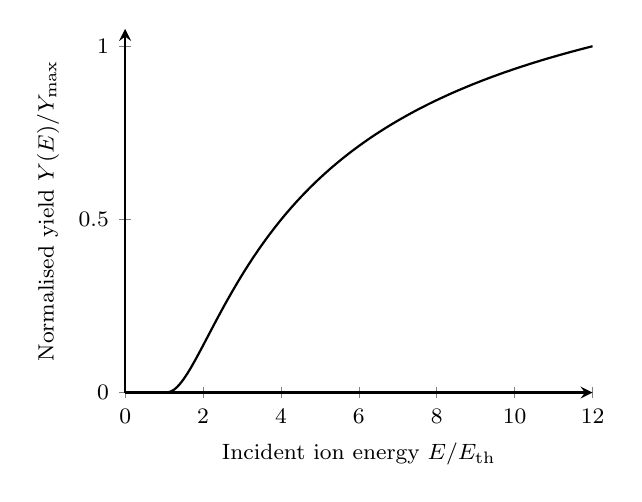
\begin{tikzpicture}
\begin{axis}[
 width=0.62\linewidth, height=6.2cm,
 xlabel={Incident ion energy $E/E_{\mathrm{th}}$},
 ylabel={Normalised yield $Y(E)/Y_{\max}$},
 xmin=0, xmax=12, ymin=0, ymax=1.05,
 domain=1:12, samples=200,
 axis lines=left,
 grid=none,
 tick label style={font=\footnotesize},
 label style={font=\footnotesize},
 line width=0.9pt,
]
\addplot[black, thick] {(1-(1/x)^(2/3))*(1-1/x)^2 / 0.68};
\end{axis}
\end{tikzpicture}
\caption{Schematic, illustrative curve of the Bohdansky-type threshold factor $[1-(E_{\mathrm{th}}/E)^{2/3}][1-E_{\mathrm{th}}/E]^{2}$ that multiplies the Sigmund nuclear-stopping yield, plotted against $E/E_{\mathrm{th}}$ and normalised to its own maximum over the plotted range. The curve is an analytic model, not measured or fitted data; it illustrates only the qualitative threshold-rise shape discussed in the text.}
\label{fig:pmi-yield-energy}
\end{figure}

Figure~\ref{fig:pmi-yield-energy} plots the dimensionless threshold factor of Equation~\eqref{eq:pmi-bohdansky} against $E/E_{\mathrm{th}}$, purely to illustrate the near-threshold rise; the true energy dependence of $Y(E)$ also carries the slowly varying $S_n(E)$ prefactor, not included in the plot.

\section{Chemical and Reactive Sputtering; Redeposition}
\label{sec:pmi-chemical}

\subsection{Chemically Enhanced Erosion}

Physical sputtering is switched off below $E_{\mathrm{th}}$, which can be tens of electronvolts for light-ion/heavy-target combinations. Many technologically important plasmas contain chemically reactive species -- oxygen, fluorine, hydrogen, and their radical derivatives -- that erode a surface by forming volatile compounds with the substrate, independent of or synergistically with ion bombardment. In chemical sputtering proper, a reactive species first forms a weakly bound surface complex; a subsequent, sub-threshold ion impact supplies enough activation energy to desorb it as a volatile molecule, so erosion proceeds well below the physical threshold with a yield that can exceed the purely physical value at the same energy. This is not confined to hydrocarbon chemistry: oxygen ion bombardment of metals produces enhanced yields, through oxide-layer formation and preferential removal of the more volatile oxidised species, and a substantial secondary-ion yield, since the electronegative oxygen adlayer lowers the ionisation barrier for sputtered atoms leaving as ions -- so measurements of only neutral or only ionised flux will systematically misestimate total erosion unless the ionised fraction is independently characterised.

A further complication: total yield per incident molecular ion is not additive in the constituent atomic yields, since correlated, closely spaced energy deposition into the same cascade produces a yield enhancement -- often superlinear in atom number -- relative to the sum expected from separate atomic ions. This is particularly relevant to hydrocarbon and hydrogen sputtering of carbon-based PFCs, and generally wherever the dominant species is molecular or a cluster ion. Physical and chemical channels are thus not simply additive; beam studies combining simultaneous ion and reactive-neutral exposure with single-channel reference measurements find synergistic enhancement factors of several times the naive sum, since ion bombardment continuously refreshes reactive sites that would otherwise passivate under neutral exposure alone.

\subsection{Redeposition and Net Erosion}

Sputtered and chemically eroded material does not vanish: it enters the plasma or vacuum environment as neutrals, molecules, and ions, a fraction of which is subsequently transported by plasma fields and neutral gas flow and redeposited elsewhere. The quantity of practical consequence is therefore never the gross yield $Y(E,\theta)$ alone but the \emph{net} erosion rate,
\begin{equation}
\Gamma_{\mathrm{net}}(\mathbf{r}) = \Gamma_{\mathrm{sputtered}}(\mathbf{r}) - \Gamma_{\mathrm{redeposited}}(\mathbf{r}).
\label{eq:pmi-neterosion}
\end{equation}
Redeposition is intrinsically a transport problem, coupling the local erosion source to the global plasma and neutral-gas flow field, and can differ dramatically between locations on the same component: regions with direct line of sight to the eroding surface accumulate redeposited material and can show net growth, while shadowed regions erode close to the gross rate. Studies of full-tungsten tokamak divertors illustrate this asymmetry starkly: gross erosion computed from ion energy flux and yield alone can overstate net material loss by a large factor where prompt redeposition is strong \cite{ref0158}. Because net, not gross, erosion limits lifetime, erosion-lifetime engineering (Section~\ref{sec:pmi-erosion-integral}) must generally couple to a redeposition model rather than be treated as purely local.

\section{Surface Heating, Thermal Loading and Secondary Electron Emission}
\label{sec:pmi-heating}

\subsection{Power Deposition by the Ion Energy Flux}

Sputtering removes only a small fraction, typically well under one percent by energy, of the power an ion delivers on impact; the great majority of $\GammaE$ is deposited as heat, through electronic and nuclear stopping, recombination with a surface electron, and the kinetic energy of secondary particles that do not escape. The surface heat flux is therefore, to good approximation, the ion energy flux itself, augmented by the electron heat flux and ionisation-potential release, reduced only marginally by sputtering and secondary-emission losses:
\begin{equation}
q_{\mathrm{surf}} \simeq \GammaE + \Gamma_i\, E_{\mathrm{iz}} + q_{e} - q_{\mathrm{SEE}} - q_{\mathrm{sput}},
\label{eq:pmi-heatbalance}
\end{equation}
where $E_{\mathrm{iz}}$ is the ionisation energy released on recombination, $q_e$ the electron contribution, and $q_{\mathrm{SEE}}$, $q_{\mathrm{sput}}$ the small losses to secondary electrons and sputtered particles. Because $\GammaE$ typically dominates Equation~\eqref{eq:pmi-heatbalance} in ion-bombarded, low-electron-temperature sheaths, direct measurement of surface heat flux gives an independent calorimetric check on the flux inferred from sheath-theoretic or probe diagnostics; heat-flux microsensors embedded in test surfaces have been used for this \cite{ref0175}. In magnetic-confinement geometries, where the flux is concentrated by field-line mapping onto narrow divertor strike regions, the resulting heat flux can dominate thermal response even for modest upstream parameters; distributing this load is a primary design driver \cite{ref0581}.

\subsection{Secondary Electron Emission and its Feedback on the Sheath}

Ion, and separately electron, bombardment releases secondary electrons through several mechanisms: potential (Auger neutralisation) emission, with no kinetic-energy threshold; kinetic emission, requiring a minimum impact energy; and, for electron-bombarded surfaces, true secondary emission from inelastic scattering. The yield $\gamma_{\mathrm{SE}}$ depends on ion species, charge state, impact energy and angle, surface composition, and -- critically for hot PFC surfaces -- temperature, since thermionic emission adds to the impact-driven yield. Secondary emission is not a passive loss channel: emitted electrons are accelerated back into the plasma by the same sheath potential that accelerated the ions inward, and a large $\gamma_{\mathrm{SE}}$ modifies the sheath's charge balance and potential profile. At surfaces hot enough to emit copiously, the outward electron current can approach or exceed the inward ion current, and the resulting "inverse" sheath changes the near-surface field and hence the effective ion impact energy for sputtering \cite{ref0038}. This feedback loop -- flux heats the surface, the hot surface modifies the sheath, and the modified sheath resets the flux -- means thermal loading and sputtering cannot, in the high-heat-flux limit, be treated as independent outputs of a fixed sheath, a concern for refractory metal PFCs.

\subsection{Transient and Steady-State Thermal Loads}

Two thermal-loading regimes must be distinguished. In steady-state operation the flux is approximately constant over timescales long compared with the thermal diffusion time, and surface temperature rises to a value set by the balance between incident heat flux and conductive (and, at high temperature, radiative) removal; actively cooled PFCs are designed around distributing this non-uniform flux to avoid hot spots \cite{ref0581}. In transient operation -- disruptions and ELMs, arcing, or pulsed thruster discharges -- the ion energy flux can rise by orders of magnitude over millisecond timescales, delivering an energy density far exceeding what steady-state conduction can remove; a small diffusion length means transient loads deposit in a thin layer, producing steep gradients and severe stress even when the time-averaged flux is modest. Pulsed electrothermal-discharge experiments reproducing disruption-like heat loads separate transient melt/vaporisation erosion from quasi-steady sputtering, since the two scale differently with pulse energy density \cite{ref0176}. Molecular-dynamics simulations further show the yield is not temperature-independent: a hotter lattice has reduced effective binding and altered defect mobility, so the same incident energy gives a different yield on a pre-heated surface, closing a second feedback loop linking thermal loading back to sputtering.

\section{Erosion as the Integral of the Ion Energy Flux}
\label{sec:pmi-erosion-integral}

\subsection{From Yield to Erosion Rate}

The instantaneous erosion rate follows directly from the yield formalism of Section~\ref{sec:pmi-physical-sputtering}. If $\Gamma_i(\mathbf{r},t)$ is the local ion flux and $\langle Y(\mathbf{r},t)\rangle$ the corresponding flux-weighted yield of Equation~\eqref{eq:pmi-yieldaverage}, the rate of surface recession is
\begin{equation}
\frac{dh}{dt}(\mathbf{r},t) = \frac{M}{\rho N_A}\, \langle Y(\mathbf{r},t)\rangle\, \Gamma_i(\mathbf{r},t),
\label{eq:pmi-erosionrate}
\end{equation}
where $M$ is the molar mass, $\rho$ the density, and $N_A$ Avogadro's constant, so $M/(\rho N_A)$ converts a number-yield into thickness removed per fluence. Total material loss over a campaign of duration $\tau$ is
\begin{equation}
\Delta h(\mathbf{r}) = \int_0^\tau \frac{dh}{dt}(\mathbf{r},t)\, dt
= \frac{M}{\rho N_A} \int_0^\tau \langle Y(\mathbf{r},t)\rangle\, \Gamma_i(\mathbf{r},t)\, dt,
\label{eq:pmi-erosionintegral}
\end{equation}
and, recasting Equation~\eqref{eq:pmi-yieldaverage} in terms of the energy-resolved flux, the same integral becomes a double integral over time and energy,
\begin{equation}
\Delta h(\mathbf{r}) = \frac{M}{\rho N_A}\int_0^\tau\!\!\int_0^\infty Y(E,\theta)\, \frac{d\Gamma_i}{dE}(\mathbf{r},E,t)\, dE\, dt.
\label{eq:pmi-erosiondouble}
\end{equation}
Equation~\eqref{eq:pmi-erosiondouble} is the formal statement that erosion is a functional of the ion energy flux delivered by the sheath: any error in characterising $d\Gamma_i/dE$ -- an incomplete kinetic model, an unresolved high-energy tail, or a diagnostic measuring only a bulk flux moment -- propagates directly, and, since $Y(E)$ is convex near threshold, often disproportionately, into erosion and lifetime prediction.

\subsection{Lifetime Estimation}

Component lifetime, in the erosion-limited sense relevant to propulsion grids, etch-chamber hardware, and fusion tiles, is the duration $\tau_{\mathrm{life}}$ at which accumulated erosion $\Delta h(\mathbf{r})$ first reaches a critical thickness $h_{\mathrm{crit}}$:
\begin{equation}
\int_0^{\tau_{\mathrm{life}}} \frac{dh}{dt}(\mathbf{r}_{\mathrm{max}},t)\, dt = h_{\mathrm{crit}},
\label{eq:pmi-lifetime}
\end{equation}
evaluated at the location $\mathbf{r}_{\mathrm{max}}$ of maximum net erosion rate. When flux and geometry are approximately steady, this reduces to $\tau_{\mathrm{life}} \approx h_0/(dh/dt)$, but should be used cautiously: yield can drift with thermal history, and redeposition can make the net rate strongly non-local. Electric propulsion illustrates the point: three-dimensional erosion models of the Hall-thruster channel wall are needed because the channel geometry evolves as erosion proceeds, reshaping the local angle and hence yield through Equation~\eqref{eq:pmi-yamamura} -- a moving-boundary problem requiring Equation~\eqref{eq:pmi-erosionrate} to be recomputed self-consistently \cite{ref0454}. Hybrid and particle-in-cell models tracking ion trajectories self-consistently give a first-principles route to the lifetime integral without an assumed, fixed distribution \cite{ref0433}. The same moving-boundary character appears in divertor assessment, where gross and net erosion and the changing field-line incidence angle at the strike point must be tracked jointly rather than assuming static geometry \cite{ref0158}.

\subsection{Erosion Diagnostics}

Because erosion-lifetime prediction depends sensitively on the fidelity of $\langle Y \rangle$ and $\Gamma_i$ inputs, direct measurement of accumulated erosion provides essential validation distinct from the flux-based modelling above. Surface-profile methods measure thickness change directly; electrical and eddy-current methods suit thin coatings. Dedicated material-testing platforms reproducing the ion energy flux, species mix, and transient heat-load character of the target application bridge laboratory measurement and full-component lifetime prediction \cite{ref0588}. Comparisons of tungsten erosion under controlled exposure against erosion predicted from tabulated yields and locally characterised flux test the flux-to-erosion chain directly, and consistently show the largest discrepancy arises not from the yield model but from incomplete characterisation of the delivered flux, reinforcing this monograph's emphasis on quantifying $\GammaE$ with high fidelity.

\begin{table}[htbp]
\centering
\caption{Qualitative ordering of the erosion-relevant regimes discussed in this chapter, collated from the cited literature to illustrate typical relative magnitudes and regime boundaries; the labels are schematic characterisations, not measured data for any specific material or device.}
\label{tab:pmi-regimes}
\begin{tabularx}{\linewidth}{@{}l l l X@{}}
\toprule
Regime & Typical $E$ range & Dominant channel & Governing quantity \\
\midrule
Sub-threshold & below $E_{\mathrm{th}}$ & chemical / reactive & surface reaction rate, not $Y(E)$ \\
Near-threshold & $\sim E_{\mathrm{th}}$--$5E_{\mathrm{th}}$ & physical, steep rise & threshold factor of Eq.~\eqref{eq:pmi-bohdansky} \\
Cascade-optimal & $\sim$ hundreds of eV--few keV & physical, near-maximal $Y$ & $S_n(E)/U_0$, Eq.~\eqref{eq:pmi-sigmund} \\
High-energy & $\gtrsim$ tens of keV & physical, declining $Y$ & ion penetration depth \\
\bottomrule
\end{tabularx}
\end{table}

\section{Material Response: Melting, Cracking and Morphology Evolution}
\label{sec:pmi-material-response}

\subsection{Melt-Layer Formation}

When the transient heat flux of Section~\ref{sec:pmi-heating} exceeds the capacity of conduction to remove heat from the near-surface layer during the pulse, local temperature can rise past the melting point, producing a thin, transient melt layer. This differs qualitatively from sputtering: whereas sputtering removes atoms individually, melt-layer erosion removes macroscopic volumes through hydrodynamic motion of the liquid -- driven by $\mathbf{J}\times\mathbf{B}$ force from induced currents, vapour-pressure recoil, and surface-tension flow -- followed by resolidification or droplet ejection. Controlled ELM-like transient heat-load experiments on candidate materials such as molybdenum show erosion per pulse increasing sharply once incident energy density crosses the melting threshold, exceeding the sputtering-only rate integrated over many quiescent pulses \cite{ref0586}. Melt-layer erosion is thus threshold-like in peak transient heat flux rather than ion impact energy, a second threshold alongside $E_{\mathrm{th}}$ of Equation~\eqref{eq:pmi-ethreshold} but triggered by the concentrated energy density of a transient event.

\subsection{Thermal Cracking and Fatigue}

Even where peak transient temperature remains below the melting point, repeated cyclic thermal loading -- steady-state operation punctuated by transients, or start-up/shutdown cycling -- drives thermally induced stress, since the heated layer is constrained by the cooler bulk beneath and cannot expand freely. When this stress exceeds the fracture strength, the surface cracks, increasing the area exposed to the plasma and creating fracture sites for subsequent cycles, so crack networks deepen and interconnect over a campaign rather than saturate at fixed depth. Studies of thermal damage in tungsten-armoured PFCs under repeated high-heat-flux loading document this progressive cracking, and in severe cases localised melting superimposed on it, identifying increased thermal resistance across the cracked layer as a self-reinforcing hazard: a cracked surface conducts heat less efficiently, so subsequent pulses drive the local peak temperature higher for the same flux \cite{ref0581}. This thermal-fatigue growth is mechanistically distinct from, but concurrent with, both melt-layer erosion and the sputtering erosion of Section~\ref{sec:pmi-erosion-integral}, so net material loss is the superposition of several coupled damage channels.

\subsection{Morphological Evolution: Ripples, Cones and Fuzz}

Prolonged ion bombardment does not, in general, leave an initially flat surface flat: the yield's dependence on local incidence angle, Equation~\eqref{eq:pmi-yamamura}, couples to the evolving topography to produce self-organised structures. Because local yield depends on local slope, a small perturbation either damps (stabilising a smooth surface) or amplifies (driving pattern formation), depending on the sign of $dY/d\theta$. Where geometry favours instability, sustained bombardment produces regular ripples of characteristic wavelength, set by competition between curvature-dependent erosion and surface diffusion.

A distinct and, for fusion, particularly consequential instability is the formation of a nanostructured, low-density "fuzz" layer on tungsten-like surfaces exposed to low-energy, high-flux helium (and helium/deuterium) bombardment. Unlike the ripple instability, fuzz formation is driven by subsurface helium bubble nucleation and growth below the sputtering threshold for helium on tungsten, so a dense population of nanometre-scale bubbles coalesces beneath the surface even though incident helium ions are individually incapable of directly sputtering the lattice; the result is a tangled network of nanofilaments with dramatically increased surface area, reduced thermal conductivity, and modified mechanical properties. Once formed, the fuzz layer's erosion and thermal response differ substantially from pristine material, so models calibrated against flat surfaces can misestimate an already-fuzzed component \cite{ref0190}. Beryllium shows an analogous fluence-dependent evolution under high-flux deuterium bombardment, including roughening, blistering, and composition changes that alter local yield and thermal-emission characteristics. In both cases morphology evolution is a feedback process that can qualitatively change the governing yield, heat-flux, and secondary-emission coefficients over a component's lifetime.

\section{Consequences for Propulsion, Etching and Fusion Hardware}
\label{sec:pmi-consequences}

\subsection{Electric Propulsion}

In gridded ion thrusters and Hall-effect thrusters, the same sheath-accelerated ion energy flux that provides thrust also erodes the hardware shaping and containing the plasma. In gridded ion optics, a small but persistent fraction of the extracted beam undergoes charge-exchange collisions with residual neutral propellant downstream of the accelerator grid, producing slow ions re-accelerated onto the grid's downstream face; striking near-normal at energies near the full accelerating potential, these drive sputtering governed by the formalism of Section~\ref{sec:pmi-physical-sputtering}, and grid-erosion evaluation methods apply the energy- and angle-resolved accounting of Section~\ref{sec:pmi-erosion-integral} to predict and validate grid lifetime against accumulated charge-exchange fluence \cite{ref0463}.

Hall-effect thrusters face an analogous but geometrically distinct problem at the discharge-channel wall, where the radial ion energy flux, accelerated axially but redirected toward the wall by the magnetic topology and near-wall sheath effects, sputters the channel liner \cite{ref0425}. Because erosion widens the channel and changes the local field mapping and hence incidence angle, it is a moving-boundary problem of the type in Section~\ref{sec:pmi-erosion-integral}, and has historically been the dominant lifetime-limiting mechanism. In-situ diagnostics of channel erosion confirm profiles predicted by three-dimensional models, closing the loop between discharge flux, angularly resolved yield, and measured erosion depth \cite{ref0454}. Hybrid and particle-in-cell simulations resolving self-consistent ion trajectories at the wall give a first-principles route to predicting erosion without an assumed distribution, directly implementing Equation~\eqref{eq:pmi-erosiondouble} for this geometry \cite{ref0433}.

\subsection{Plasma Etching and Surface Processing}

In plasma etching, the same ion energy flux that erodes propulsion hardware is deliberately engineered to remove material from a wafer or substrate in a controlled, patterned way. Two regimes are exploited. In sputter-cleaning, low-energy bombardment near or just above the physical-sputtering threshold removes a thin, controlled amount of surface material -- native oxide, contamination, or a sacrificial layer -- without the lattice damage of higher-energy bombardment. At the other extreme, reactive ion etching combines the chemical erosion channels of Section~\ref{sec:pmi-chemical} with directed ion bombardment to achieve highly anisotropic removal: the reactive neutral flux etches isotropically wherever it reaches bare surface, but proceeds far faster on ion-bombarded horizontal surfaces than on ion-shadowed sidewalls, so the combination produces the vertical, high-aspect-ratio profiles required by modern microfabrication \cite{ref0536}.

\subsection{Fusion Plasma-Facing Components}

Magnetic confinement fusion presents the most demanding plasma-surface interaction environment in this chapter, combining the highest steady-state ion energy fluxes, the most severe transient heat loads, and the longest required lifetimes of any application discussed. Materials-screening for fusion PFCs must evaluate physical sputtering threshold behaviour, chemical erosion under the reactive isotopic mix (deuterium, tritium, helium ash) at a burning-plasma edge, thermal shock tolerance, and the morphology pathways of Section~\ref{sec:pmi-material-response}, since no single candidate -- tungsten, beryllium, carbon-based options -- dominates on every axis \cite{ref0189}. The resulting challenges span material selection, active-cooling design built around the heat-flux distributions of Section~\ref{sec:pmi-heating}, and erosion-lifetime qualification built on the flux-integral formalism of Section~\ref{sec:pmi-erosion-integral}, since PFCs must survive combined steady-state and transient loading over a full campaign in the least accessible locations. Because disruptions can deposit an enormous energy density on a millisecond timescale, disruption heat-load modelling incorporates the vapour-shielding effect, in which early-ablated material forms a dense vapour layer that absorbs and re-radiates a substantial fraction of the incoming energy, self-limiting -- though not eliminating -- net erosion during severe events \cite{ref0176}. Non-invasive diagnostics, such as spectroscopic monitoring of neutral tungsten emission as a proxy for gross erosion, provide shot-by-shot tracking that closes the loop between model and measured erosion.

\section*{Summary}
\addcontentsline{toc}{section}{Summary}

This chapter has traced the consequences of the ion energy flux $\GammaE$ delivered by the plasma sheath once it reaches a material surface. Physical sputtering is governed by a threshold energy set, to leading order, by binary-collision kinematics (Equation~\eqref{eq:pmi-ethreshold}), with the yield above threshold described by Sigmund's linear-cascade theory (Equation~\eqref{eq:pmi-sigmund}) and its threshold-corrected Bohdansky extension (Equation~\eqref{eq:pmi-bohdansky}), and a rise-then-fall angular dependence (Equation~\eqref{eq:pmi-yamamura}) that couples to surface geometry and, over time, to the surface's own evolving morphology. Chemical channels extend removal below the physical threshold and interact synergistically, rather than additively, with ion bombardment, while redeposition transforms the local gross yield into a globally coupled net erosion rate. Energy not carried away by sputtered particles is deposited as surface heat, driving secondary electron emission that feeds back on the sheath and, in transient events, melting and cracking that act as damage channels distinct from, and superimposed upon, sputtering erosion. Erosion and thermal loading were both cast as functionals of the energy-resolved ion flux, $d\Gamma_i/dE$ (Equation~\eqref{eq:pmi-erosiondouble}), making explicit that any deficiency in characterising the ion energy flux -- the central quantity of this monograph -- propagates directly, and often disproportionately near threshold, into erosion, lifetime, and thermal-damage predictions. These consequences were traced through three domains: electric propulsion, plasma etching, and fusion plasma-facing components.


\part{Measurement and Modelling}
\chapter{Intrusive Diagnostics and Their Limitations}
\label{ch:probes}

The quantification of ion energy flux across a plasma sheath has historically been approached through diagnostics that place a solid object directly into the plasma and interpret the currents, voltages, or particle fluxes it collects. Electrostatic (Langmuir) probes, retarding-field energy analyzers, and their derivatives remain the most widely deployed tools for measuring electron temperature, plasma density, plasma potential, and ion energy distributions. Their appeal is clear: inexpensive, mechanically simple, high-resolution, and grounded in a century-old analytic theory. Yet every intrusive probe measurement is, by construction, a measurement of a plasma locally modified by the probe itself: it nucleates its own sheath, draws a compensating return current, and in high-flux or magnetized environments may not survive the flux it is meant to quantify. This chapter develops the theory of electrostatic probe diagnostics, catalogs the principal probe geometries, and then turns critically to three limitations motivating the non-intrusive alternatives pursued later: perturbation from probe-sheath formation, physical degradation in high-flux environments, and interpretive ambiguities in non-Maxwellian or magnetized plasmas.

\section{Langmuir Probe Theory}
\label{sec:probes-langmuir-theory}

\subsection{Historical Basis and the Collected Current}

The electrostatic probe technique originates with Langmuir's analysis of the current collected by a small biased electrode in a low-temperature discharge, and remains the most direct method for extracting local electron density, temperature, and plasma potential; refined slope-extraction procedures continue to convert Langmuir's original graphical method into forms suitable for automated data reduction \cite{ref0217}.

A probe of collecting area $A_{\mathrm{p}}$ immersed in a plasma and biased to a voltage $V$ relative to a fixed reference collects a net current
\begin{equation}
I(V) = I_{\mathrm{e}}(V) - I_{\mathrm{i}}(V),
\label{eq:probe-net-current}
\end{equation}
where $I_{\mathrm{i}}(V)$ and $I_{\mathrm{e}}(V)$ are the ion and electron currents at that bias, positive net current corresponding to net electron collection. Sweeping $V$ across several electron temperatures on either side of $\phi_{\mathrm{p}}$ generates the characteristic Langmuir I-V trace, divided into three regions: ion saturation at strongly negative bias, the exponential (transition) region at intermediate bias, and electron saturation near or above $\phi_{\mathrm{p}}$.

\subsection{The Exponential Transition Region and Electron Temperature}

In the transition region, the probe is negative enough relative to $\phi_{\mathrm{p}}$ that only the high-energy tail of the electron velocity distribution has enough directed kinetic energy to overcome the retarding potential. For an electron population locally Maxwellian at temperature $T_{\mathrm{e}}$, the retarded current takes the Boltzmann form:
\begin{equation}
I_{\mathrm{e}}(V) = I_{\mathrm{es}} \, \exp\!\left[-\frac{e\left(\phi_{\mathrm{p}} - V\right)}{k_{\mathrm{B}} T_{\mathrm{e}}}\right], \qquad V \le \phi_{\mathrm{p}},
\label{eq:probe-exp-region}
\end{equation}
where $I_{\mathrm{es}}$ is the electron saturation current at $V = \phi_{\mathrm{p}}$. This is the single most consequential relation in probe theory, converting the slope of the electron current on a semi-logarithmic plot into a direct measurement of electron temperature:
\begin{equation}
\frac{\mathrm{d}\,\ln I_{\mathrm{e}}}{\mathrm{d}V} = \frac{e}{k_{\mathrm{B}} T_{\mathrm{e}}}
\quad\Longrightarrow\quad
T_{\mathrm{e}} = \frac{e}{k_{\mathrm{B}}} \left(\frac{\mathrm{d}\,\ln I_{\mathrm{e}}}{\mathrm{d}V}\right)^{-1}.
\label{eq:probe-Te-slope}
\end{equation}
Extracting $I_{\mathrm{e}}(V)$ from the raw trace requires subtracting a weakly voltage-dependent ion current; the subtraction method chosen (constant, linear extrapolation, or sheath-expansion model) is a recurring source of disagreement between nominally identical measurements \cite{ref0217}.

\subsection{Saturation Currents and the Extraction of Density}

At bias well above $\phi_{\mathrm{p}}$, the probe collects the random thermal flux of electrons crossing an unperturbed interface, giving the electron saturation current
\begin{equation}
I_{\mathrm{es}} = \frac{1}{4} n_{\mathrm{e}} e \, \bar{v}_{\mathrm{e}} \, A_{\mathrm{p}}, \qquad
\bar{v}_{\mathrm{e}} = \sqrt{\frac{8 k_{\mathrm{B}} T_{\mathrm{e}}}{\pi m_{\mathrm{e}}}},
\label{eq:probe-Ies}
\end{equation}
which, once $T_{\mathrm{e}}$ is known from Equation~\eqref{eq:probe-Te-slope}, yields $n_{\mathrm{e}}$ directly. In practice this branch is rarely used, since it is strongly distorted by sheath expansion, secondary emission, and (in bounded or magnetized geometries) depletion of the primary electron population; the ion-saturation branch is generally preferred. At strongly negative bias, ions accelerate to the Bohm velocity crossing the sheath edge, and the collected ion current saturates near
\begin{equation}
I_{\mathrm{is}} \simeq e\, n_{\mathrm{s}}\, u_{\mathrm{B}} \, A_{\mathrm{p}}, \qquad
u_{\mathrm{B}} = \sqrt{\frac{k_{\mathrm{B}} T_{\mathrm{e}}}{m_{\mathrm{i}}}},
\label{eq:probe-Iis}
\end{equation}
where $n_{\mathrm{s}} \approx 0.6\, n_{\mathrm{e}}$ is the sheath-edge ion density, reduced below bulk by the presheath density drop. Because $u_{\mathrm{B}}$ depends only on $T_{\mathrm{e}}$ and ion mass, Equation~\eqref{eq:probe-Iis} gives a comparatively robust route to density even where electron saturation is unreliable, though in flowing or high-density sources this assumption breaks down once drift velocities approach thermal speeds.

\subsection{Plasma Potential and Floating Potential}

The plasma (space) potential $\phi_{\mathrm{p}}$ marks the transition between the exponential region and the saturation region above it, formally the bias where $\mathrm{d}^2 I / \mathrm{d}V^2 = 0$, the "knee" of the I-V trace. In an idealized planar geometry with a strictly Maxwellian population this knee is sharp; in real probes it is rounded by sheath expansion, tip geometry, and non-thermal admixture, making $\phi_{\mathrm{p}}$ delicate to locate. The more easily measured floating potential $V_{\mathrm{f}}$, where $I(V_{\mathrm{f}}) = 0$, follows from Equations~\eqref{eq:probe-exp-region} and~\eqref{eq:probe-Ies}--\eqref{eq:probe-Iis} as
\begin{equation}
V_{\mathrm{f}} = \phi_{\mathrm{p}} - \frac{k_{\mathrm{B}} T_{\mathrm{e}}}{e} \ln\!\left(\frac{I_{\mathrm{es}}}{I_{\mathrm{is}}}\right),
\label{eq:probe-Vf}
\end{equation}
so the offset between plasma and floating potential is set entirely by the electron-to-ion saturation current ratio, itself a function of $T_{\mathrm{e}}$, $T_{\mathrm{i}}$, and ion mass. A self-consistent joint measurement of $\phi_{\mathrm{p}}$, $T_{\mathrm{e}}$, and the electron energy distribution from a single trace has been demonstrated in tokamak edge plasma, illustrating the power of the full I-V characteristic and the care needed when the edge population departs from Maxwellian \cite{ref0213}.

Table~\ref{tab:probe-quantities} summarizes the quantities recoverable from a single swept trace.

\begin{table}[htbp]
\centering
\caption{Plasma parameters recovered from a single swept Langmuir probe characteristic, and the region of the I-V trace from which each is extracted.}
\label{tab:probe-quantities}
\begin{tabularx}{\textwidth}{@{}l l X@{}}
\toprule
Quantity & Symbol & Extraction region / method \\
\midrule
Electron temperature & $T_{\mathrm{e}}$ & Slope of $\ln I_{\mathrm{e}}$ in the exponential (transition) region, Eq.~\eqref{eq:probe-Te-slope} \\
Electron density & $n_{\mathrm{e}}$ & Electron saturation current $I_{\mathrm{es}}$, Eq.~\eqref{eq:probe-Ies}, combined with $T_{\mathrm{e}}$ \\
Ion density at sheath edge & $n_{\mathrm{s}}$ & Ion saturation current $I_{\mathrm{is}}$, Eq.~\eqref{eq:probe-Iis}, combined with $T_{\mathrm{e}}$ \\
Plasma potential & $\phi_{\mathrm{p}}$ & Knee of the I-V trace, $\mathrm{d}^2 I/\mathrm{d}V^2 = 0$ \\
Floating potential & $V_{\mathrm{f}}$ & Zero-current crossing, Eq.~\eqref{eq:probe-Vf} \\
Electron energy distribution & $f_{\mathrm{e}}(E)$ & Second derivative $\mathrm{d}^2 I_{\mathrm{e}}/\mathrm{d}V^2$ (Druyvesteyn method) \\
\bottomrule
\end{tabularx}
\end{table}

\section{Single, Double and Emissive Probes; Retarding-Field Energy Analyzers}
\label{sec:probes-variants}

\subsection{The Single (Swept) Probe}

The single probe, described above, is the simplest configuration: one electrode, referenced to a fixed potential such as chamber ground, swept in bias while its current is recorded. Its main disadvantage is that it requires a stable reference and draws substantial electron current near $\phi_{\mathrm{p}}$, which can perturb weakly ionized or low-power discharges and is impractical where no grounded reference exists.

\subsection{Double Probes}

The double-probe technique replaces the single grounded reference with a second, electrically isolated tip, sweeping a bias between the two electrodes rather than between one electrode and ground. Because the pair floats together, the sum of the two collected currents stays small: both electrodes remain near their local floating potential and the current saturates at the ion-saturation level in both directions. For two equal-area electrodes at equal $T_{\mathrm{e}}$, the symmetric characteristic is
\begin{equation}
I(V) = I_{\mathrm{is}} \tanh\!\left(\frac{eV}{2 k_{\mathrm{B}} T_{\mathrm{e}}}\right),
\label{eq:double-probe}
\end{equation}
where $V$ is the voltage between the two tips. Equation~\eqref{eq:double-probe} never exhibits an electron-saturation branch; the technique trades access to $\phi_{\mathrm{p}}$ and $I_{\mathrm{es}}$-based density for immunity to a floating or time-varying reference, keeping the essential thermometric capability of the single-probe method.

\subsection{Triple Probes}

The triple probe extends the double-probe idea to a single, instantaneous (unswept) determination of $T_{\mathrm{e}}$ and $n_{\mathrm{e}}$, essential where a voltage sweep cannot be completed within the plasma's evolution time. Three electrodes are used: one floats freely, and the other two are held at a fixed $\Delta V$ large enough to drive one into ion saturation. The floating electrode provides $V_{\mathrm{f}}$, the biased pair provides one point on the exponential branch plus the ion-saturation current, and $T_{\mathrm{e}}$ follows algebraically without a sweep, making the triple probe the configuration of choice in fast-evolving or single-shot plasmas.

\subsection{Emissive Probes}

All configurations above share a common limitation: a cold, electron-collecting probe biased near $\phi_{\mathrm{p}}$ still perturbs the local sheath, and the rounded I-V knee introduces an ambiguity of several electron temperatures. The emissive probe addresses this by heating a fine filament (typically thoriated tungsten) to drive thermionic emission. When biased below $\phi_{\mathrm{p}}$, the sheath that would otherwise repel plasma electrons instead accelerates the probe's own emitted electrons away from the filament; as emitted current rises, the floating potential asymptotically approaches $\phi_{\mathrm{p}}$ itself, since a probe emitting electrons as readily as the plasma emits electrons toward it no longer needs a repulsive sheath to balance currents. $\phi_{\mathrm{p}}$ is then obtained from the inflection point of the probe's trace, or by extrapolating floating potential to zero net emission, both less sensitive to the electron distribution than the cold-probe knee method. Recommended-practice guidelines for electric propulsion testing discuss emissive probes and RFEAs alongside Langmuir probes, since thruster-plume measurements routinely require cross-checking with more than one probe type \cite{ref0226}.

\subsection{Retarding-Field Energy Analyzers}

Where a Langmuir probe measures moments of the electron velocity distribution, a retarding-field energy analyzer (RFEA) reconstructs the ion energy distribution function $f_{\mathrm{i}}(v)$ directly, making it the intrusive instrument most directly relevant to $\Gamma_{E}$. An RFEA admits plasma through a small orifice into a sheath-isolated interior, where a sequence of biased grids filters successively: a floating entrance grid, a repeller grid rejecting electrons, a discriminator grid swept positive to select ions of sufficient axial energy, and a suppressor grid rejecting secondary electrons from the collector. The collected current as a function of discriminator voltage $V_{\mathrm{d}}$ is the integral of ion flux above the corresponding energy threshold,
\begin{equation}
I_{\mathrm{coll}}(V_{\mathrm{d}}) = e A_{\mathrm{ap}} \int_{v_{\min}(V_{\mathrm{d}})}^{\infty} v\, f_{\mathrm{i}}(v)\, \mathrm{d}v,
\qquad
\tfrac{1}{2} m_{\mathrm{i}} v_{\min}^2 = e V_{\mathrm{d}},
\label{eq:rfea-collected}
\end{equation}
where $A_{\mathrm{ap}}$ is the effective aperture area. Differentiating with respect to $V_{\mathrm{d}}$ recovers $f_{\mathrm{i}}$ directly,
\begin{equation}
\frac{\mathrm{d}I_{\mathrm{coll}}}{\mathrm{d}V_{\mathrm{d}}} \;\propto\; f_{\mathrm{i}}(v)\Big|_{v = v_{\min}(V_{\mathrm{d}})},
\label{eq:rfea-derivative}
\end{equation}
and once $f_{\mathrm{i}}(v)$ is known, the ion energy flux delivered to the aperture follows as the first energy moment,
\begin{equation}
\Gamma_{E} = \int_0^\infty E\, f_{\mathrm{i}}(E) \, \mathrm{d}E .
\label{eq:rfea-gammaE}
\end{equation}
The RFEA is thus, in principle, the most direct intrusive route to the quantity this monograph seeks to quantify non-invasively. In practice, though, the finite transparency of each grid (40-80 percent, compounding across four grids) suppresses the signal and introduces energy-dependent transmission losses requiring calibration. The orifice acts as a miniature aperture sheath whose Debye length must be resolved by the hole diameter, and at high density the ion flow can become space-charge limited, distorting the measured distribution in the high-flux regime of greatest interest here, as in scrape-off-layer measurements at a divertor target that recover ion temperature from the retarding-field characteristic itself \cite{ref0610}.

\section{The Probe Sheath and Perturbation of the Measured Plasma}
\label{sec:probes-sheath-perturbation}

\subsection{Sheath Formation at the Probe Surface}

Any electrode biased away from $\phi_{\mathrm{p}}$ nucleates its own Debye sheath, structurally identical in kind (though not in scale) to the wall sheath discussed elsewhere. Quasineutrality is violated within a layer whose thickness is set by the electron Debye length,
\begin{equation}
\lambda_{\mathrm{D}} = \sqrt{\frac{\varepsilon_0 k_{\mathrm{B}} T_{\mathrm{e}}}{n_{\mathrm{e}} e^2}},
\label{eq:probe-debye}
\end{equation}
and ions entering this layer from the quasineutral bulk must already possess, at the sheath edge, a directed velocity of at least $u_{\mathrm{B}}$ (Equation~\eqref{eq:probe-Iis}), accelerated across a presheath in which density falls to $n_{\mathrm{s}} \approx 0.6\,n_{\mathrm{e}}$. For a probe biased substantially negative of $\phi_{\mathrm{p}}$, the sheath is a space-charge-limited, ion-dominated layer whose thickness follows the Child-Langmuir law,
\begin{equation}
s \;\sim\; \lambda_{\mathrm{D}} \frac{\sqrt{2}}{3}\left(\frac{2e\left|\phi_{\mathrm{p}} - V\right|}{k_{\mathrm{B}} T_{\mathrm{e}}}\right)^{3/4},
\label{eq:probe-child-langmuir}
\end{equation}
so that at strongly negative bias the sheath can grow to many Debye lengths. Figure~\ref{fig:probe-sheath-schematic} depicts this structure schematically.

\begin{figure}[htbp]
\centering
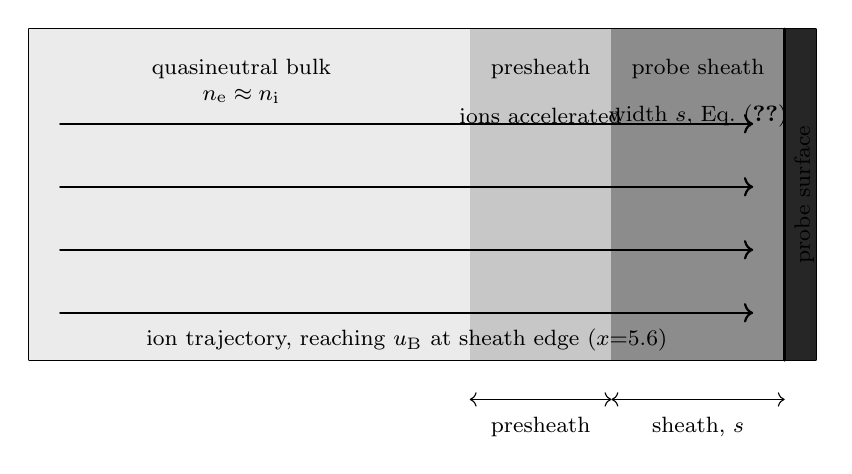
\begin{tikzpicture}[x=1cm,y=1cm,line cap=round,line join=round]

 \draw[thick] (0,0) rectangle (10,4.2);

 \fill[black!8] (0,0) rectangle (5.6,4.2);
 \fill[black!22] (5.6,0) rectangle (7.4,4.2);
 \fill[black!45] (7.4,0) rectangle (9.6,4.2);
 \fill[black!85] (9.6,0) rectangle (10,4.2);

 \draw[very thick] (9.6,0) -- (9.6,4.2);

 \node at (2.7,3.7) {\footnotesize quasineutral bulk};
 \node at (2.7,3.35) {\footnotesize $n_{\mathrm{e}} \approx n_{\mathrm{i}}$};

 \node at (6.5,3.7) {\footnotesize presheath};
 \node[align=center] at (6.5,3.1) {\footnotesize ions accelerated};

 \node at (8.5,3.7) {\footnotesize probe sheath};
 \node[align=center] at (8.5,3.1) {\footnotesize width $s$, Eq.~\eqref{eq:probe-child-langmuir}};

 \node[rotate=90] at (9.85,2.1) {\footnotesize probe surface};

 \foreach \y in {0.6,1.4,2.2,3.0}{
 \draw[->,thick] (0.4,\y) -- (9.2,\y);
 }
 \node at (4.8,0.25) {\footnotesize ion trajectory, reaching $u_{\mathrm{B}}$ at sheath edge ($x{=}5.6$)};

 \draw[<->] (5.6,-0.5) -- (7.4,-0.5);
 \node at (6.5,-0.85) {\footnotesize presheath};
 \draw[<->] (7.4,-0.5) -- (9.6,-0.5);
 \node at (8.5,-0.85) {\footnotesize sheath, $s$};

\end{tikzpicture}
\caption{Schematic cross-section of the presheath and sheath adjacent to a negatively biased planar probe surface. Shading darkens toward the probe surface, indicating progressive departure from quasineutrality; ion trajectories (arrows) accelerate through the presheath and cross the sheath edge at approximately the Bohm velocity $u_{\mathrm{B}}$. No experimental data are represented; the figure is a conceptual aid only.}
\label{fig:probe-sheath-schematic}
\end{figure}

\subsection{Sheath Expansion, Effective Collection Area, and Orbit-Limited Collection}

A subtlety with direct consequences for density extraction: the probe's effective collecting area is not, in general, its physical geometric area, because the sheath boundary expands outward as bias is driven more negative, per Equation~\eqref{eq:probe-child-langmuir}. For a planar probe this is often small; but for the cylindrical or spherical tips used in most laboratory probes, sheath expansion increases the effective collecting area with bias, producing an ion-saturation branch that fails to saturate cleanly, a departure from the idealized flat saturation implicit in Equation~\eqref{eq:probe-Iis}. When the probe radius is comparable to or smaller than the sheath thickness, ion collection is better described by orbital-motion-limited (OML) theory, in which ions with sufficient angular momentum are deflected around the probe without being collected; the choice among planar, cylindrical, and OML collection models is itself a nontrivial source of uncertainty in the inferred density.

\subsection{Global Perturbation of the Bulk Plasma}

Beyond the local sheath, the probe perturbs the plasma non-locally: any current it draws must be returned through some other conducting surface, whether the chamber wall or a partner tip; this return current modifies the ambipolar balance near both the probe and its return path, significant when the probe occupies a non-negligible fraction of the plasma volume or draws electron-saturation current comparable to the discharge current. In small or low-power sources this is not a second-order correction: gyrofluid-simulation-based studies show the collected current is sensitive to the assumed background temperature profile in ways a purely local, unperturbed-plasma interpretation cannot capture \cite{ref0194}.

\section{Survival, Contamination, and Erosion in High-Flux Environments}
\label{sec:probes-survival}

\subsection{Thermal and Sputtering Loads}

The very high-flux, high-energy environments where ion energy flux quantification is most urgently needed, magnetized fusion edge and divertor plasmas, high-power-density processing reactors, and thruster plumes, are also the environments most hostile to a solid probe tip. A probe surface immersed there is subject simultaneously to Joule heating from the collected current, kinetic heating from ion bombardment, and physical sputtering that erodes the surface and alters its geometry over a single sweep or campaign. Because the ion energy delivered to the probe is set by the same sheath acceleration this monograph seeks to quantify, a probe deployed to measure high ion energy flux is unavoidably subjected to that flux as a material load, forcing rapid sweeps and tight duty-cycling so cumulative damage does not compromise tip geometry within a single measurement.

\subsection{Contamination and Its Effect on the Collected Characteristic}

A second, subtler failure mode is surface contamination: deposition of sputtered material, condensable reaction products, or dielectric films, which changes the effective work function and, in the worst case, forms a partially insulating layer that rectifies the collected current asymmetrically between bias polarities. A contaminated probe can produce an I-V trace that appears smooth and reasonable while yielding a systematically biased $T_{\mathrm{e}}$ or $n_{\mathrm{e}}$, since Equation~\eqref{eq:probe-exp-region} implicitly assumes a work function and secondary-electron yield constant across the sweep and known a priori. This is acute in laser-produced and ablation plasmas, where ablated material can coat the tip between shots, necessitating frequent conditioning or replacement. In reactive or dusty discharges, similar concerns motivate cross-validation of probe-derived $T_{\mathrm{e}}$ and $n_{\mathrm{e}}$ against independent, non-contact techniques (Section~\ref{sec:probes-alternatives}).

\subsection{Duty-Cycled and Transient Operation}

Where continuous exposure is impractical, probes are duty-cycled: inserted briefly into the high-flux region, swept, and withdrawn before cumulative erosion or thermal loading becomes significant, or operated only during a single transient pulse. Triple-probe systems, requiring no sweep, suit this mode particularly well. In all such cases, the diagnostic strategy is fundamentally a compromise between the resolution demanded by the physics and the survivability of the sensor, a compromise that becomes less favorable as ion energy flux increases, precisely the regime of greatest interest here.

\section{Interpretation Ambiguities in Non-Maxwellian and Magnetized Plasmas}
\label{sec:probes-ambiguities}

\subsection{Departures from a Maxwellian Electron Energy Distribution}

The entire derivation in Section~\ref{sec:probes-langmuir-theory}, from Equation~\eqref{eq:probe-exp-region} to the slope-based extraction of $T_{\mathrm{e}}$ in Equation~\eqref{eq:probe-Te-slope}, rests on the assumption that the electron population feeding the probe sheath is locally Maxwellian. This fails routinely in low-pressure, non-equilibrium discharges, where the electron energy distribution commonly exhibits a bi-Maxwellian structure (a cold bulk plus a hotter tail sustained by discharge heating), a depleted high-energy tail, or a power-law kappa tail more familiar from space plasmas. When the true distribution is non-Maxwellian, a single-slope fit to $\ln I_{\mathrm{e}}(V)$ no longer yields a well-defined temperature: the slope varies with bias, and the reported "electron temperature" depends on the fit window, an ambiguity with no general resolution short of recovering the full distribution. The more rigorous alternative is the Druyvesteyn method, inverting the distribution directly from the second derivative of the retarded current,
\begin{equation}
f_{\mathrm{e}}(E) \;\propto\; \sqrt{E}\; \frac{\mathrm{d}^2 I_{\mathrm{e}}}{\mathrm{d}V^2}, \qquad E = e\left(\phi_{\mathrm{p}} - V\right),
\label{eq:druyvesteyn}
\end{equation}
at the cost of extreme noise sensitivity, since numerical second differentiation amplifies high-frequency noise in the raw trace. Joint measurements of the electron energy distribution, plasma potential, and density from a single trace in tokamak edge plasma demonstrate both the payoff of extracting the full distribution and the added complexity this requires relative to a simple two-parameter Maxwellian fit \cite{ref0213}.

\subsection{Fluctuation-Induced Bias}

A related, underappreciated source of error arises when plasma parameters fluctuate on timescales comparable to or shorter than the sweep time. Because Equation~\eqref{eq:probe-exp-region} is nonlinear in both $T_{\mathrm{e}}$ and $\phi_{\mathrm{p}}$, a time-averaged I-V trace acquired during a fluctuating plasma does not, in general, correspond to the time-averaged parameters; Jensen's inequality guarantees that averaging a convex function of a fluctuating quantity biases the result relative to evaluating that function at the mean. This is especially acute in scrape-off-layer turbulence studies, where probes resolve correlation lengths of intermittent structures, and where fluctuation statistics measured across devices such as Alcator C-Mod provide a benchmark against which probe-inferred correlation lengths must be interpreted with this bias in mind \cite{ref0611}.

\subsection{Magnetized Plasmas and Anisotropic Collection}

A strong background magnetic field introduces a further, qualitatively distinct difficulty: charged-particle collection becomes intrinsically anisotropic, since electrons and ions gyrate about field lines with gyroradii comparable to, larger than, or smaller than the probe dimension and sheath thickness. When the electron gyroradius is small compared with the probe and sheath, collection along the field is strongly enhanced relative to collection across field lines, and the isotropic expression underlying Equation~\eqref{eq:probe-Ies} must be replaced by an angle- and field-dependent model; probe orientation relative to $\mathbf{B}$ becomes an experimental variable itself. At the sheath itself, an oblique field modifies the ion acceleration and effective Bohm criterion relative to the unmagnetized case (Section~\ref{sec:probes-sheath-perturbation}), so a model calibrated against unmagnetized theory can misattribute magnetic effects to spurious changes in $T_{\mathrm{e}}$ or $n_{\mathrm{e}}$.

\subsection{Collisional and Orbit-Limited Corrections}

Even absent a magnetic field, the idealized collisionless, planar sheath model underlying Equations~\eqref{eq:probe-exp-region}--\eqref{eq:probe-child-langmuir} can fail once the sheath or presheath thickness becomes comparable to the ion- or electron-neutral mean free path, a regime found in higher-pressure processing plasmas and dense, partially ionized sources. Collisions randomize ion trajectories that would otherwise cross ballistically, softening the sharp saturation predicted by orbit-limited or Child-Langmuir theory and adding the mean free path as an extra free parameter. Comparative studies across multiple probe configurations under identical conditions are needed to isolate genuine physics from artifacts of the collection-theory assumptions; no single analytic probe theory can be trusted in isolation.

\section{The Case for Non-Intrusive Alternatives}
\label{sec:probes-alternatives}

The preceding sections establish a consistent pattern: every strength of the Langmuir probe and its derivatives, direct current collection, simple theory, high resolution, is coupled to an equally direct vulnerability, because the measurement mechanism is inseparable from the physical presence of a biased electrode in the plasma. The probe sheath perturbs the local ambipolar balance (Section~\ref{sec:probes-sheath-perturbation}); the probe surface is degraded by the same high-energy ion flux it is deployed to measure (Section~\ref{sec:probes-survival}); and the interpretation of the collected current becomes ambiguous precisely in the non-Maxwellian, magnetized, and collisional regimes that characterize many plasmas of greatest interest (Section~\ref{sec:probes-ambiguities}). None of these is a matter of instrumental refinement that further engineering can eliminate; they follow from the fact that probe theory presupposes a well-characterized sheath and electron distribution, exactly the quantities least certain under the most demanding conditions.

This has motivated a sustained effort to cross-validate, and where possible replace, electrostatic probe measurements with diagnostics that do not require inserting a material object into the plasma. Optical techniques that infer $T_{\mathrm{e}}$ and $n_{\mathrm{e}}$ from the plasma's own radiated or scattered light are the most direct alternative, and a substantial body of work has benchmarked these methods against Langmuir probes under matched conditions, with discrepancies traceable to exactly the perturbation and non-Maxwellian effects discussed above \cite{ref0237}. Comparable cross-validation between Langmuir probes and laser Thomson scattering, which infers $T_{\mathrm{e}}$ and $n_{\mathrm{e}}$ from the Doppler-broadened spectrum of light scattered incoherently from free electrons without any sheath assumption, has been carried out in Hall-effect plasma sources, a regime combining high power density with strong non-uniformity in which probe survivability and interpretation are both challenged \cite{ref0355}. Broader comparisons reinforce the finding that the two techniques agree well in benign, near-Maxwellian, weakly perturbed plasmas but diverge as conditions approach the regimes identified in Section~\ref{sec:probes-ambiguities} \cite{ref0354}, and foundational treatments of Thomson-scattering theory establish the conditions under which the scattered spectrum can be inverted for $n_{\mathrm{e}}$ and $T_{\mathrm{e}}$ without the sheath-based assumptions underlying every probe method in this chapter \cite{ref0384}.

Taken together, this literature supports two conclusions motivating the remainder of this monograph. First, electrostatic probes and RFEAs remain indispensable where their limitations are well characterized and the operating regime is benign: low-flux, weakly magnetized, near-Maxwellian plasmas at modest density, where the sheath model of Section~\ref{sec:probes-sheath-perturbation} is trustworthy and the probe survives long enough to complete a measurement. Second, and more important here, the plasmas of greatest practical interest, those with high ion energy flux across the sheath, are systematically the plasmas in which intrusive measurements are least reliable, because high flux threatens probe survival, drives the sheath and presheath into regimes where simple collection theory breaks down, and is often associated with non-Maxwellian or magnetized conditions. This inverse relationship between measurement difficulty and diagnostic reliability establishes the case, developed in the chapters that follow, for characterizing ion energy flux without placing a solid, current-collecting object into the sheath being measured.

\section{Summary}
\label{sec:probes-summary}

This chapter developed the theoretical basis of electrostatic probe diagnostics, from the exponential I-V characteristic and its use in extracting $T_{\mathrm{e}}$, $n_{\mathrm{e}}$, and $\phi_{\mathrm{p}}$ (Section~\ref{sec:probes-langmuir-theory}), through the principal probe geometries and the RFEA used to reconstruct $f_{\mathrm{i}}(v)$ and $\Gamma_{E}$ directly (Section~\ref{sec:probes-variants}). It then examined the sheath that inevitably forms around any biased probe surface, its Child-Langmuir scaling, and the resulting local and global perturbation of the measured plasma (Section~\ref{sec:probes-sheath-perturbation}), before turning to high-flux operation, where thermal loading, sputtering erosion, and contamination progressively degrade fidelity and threaten survival (Section~\ref{sec:probes-survival}). The chapter's central difficulty, developed in Section~\ref{sec:probes-ambiguities}, is that the interpretive framework underlying every probe method presupposes a Maxwellian, unmagnetized, collisionless plasma, an assumption that fails precisely in the non-equilibrium, magnetized, collisional regimes most relevant to modern plasma technology and fusion-edge research. The comparative evidence in Section~\ref{sec:probes-alternatives}, drawn from benchmarking against optical and Thomson-scattering techniques, shows these limitations to be structural rather than instrumental, growing most severe exactly where $\Gamma_E$ is largest, setting the stage for the non-intrusive diagnostic strategies developed in the chapters that follow.

\chapter{Optical Emission Spectroscopy}
\label{ch:oes}

Optical emission spectroscopy (OES) occupies a distinctive place in the diagnostic hierarchy of this monograph. Every technique treated so far — the Langmuir probe, laser-induced fluorescence, the retarding-field energy analyser — perturbs the plasma, either by inserting a material collector into the sheath-forming boundary layer or by driving a resonant transition with an external laser. OES is different: it collects light the plasma emits of its own accord, without a probe tip, biasing, or external energy deposition. This passivity is both its greatest strength and its principal interpretive difficulty. Because no probe perturbs the local field or velocity distribution, $T_{\mathrm{e}}$ and $n_{\mathrm{e}}$ inferred from a line-intensity ratio are, in principle, undistorted values of the bulk-plasma or presheath conditions. But because the measured quantity is a photon flux integrated along a line of sight, and the excited-state population results from competition among many collisional and radiative channels, extracting $T_{\mathrm{e}}$ and $n_{\mathrm{e}}$ from raw intensities requires an atomic-physics model as sophisticated as the sheath models developed earlier. This chapter builds that model — the collisional-radiative (CR) framework — from first principles, connects it to the practical line-ratio and actinometric extraction methods, surveys the instrumentation and calibration enabling quantitative spectroscopy, and closes by placing OES within the multi-diagnostic strategy used here to constrain the ion energy flux $\Gamma_{E}$ across the plasma sheath.

\section{Emission Physics of Low-Temperature Plasmas}

\subsection{Elementary excitation and de-excitation channels}

The light collected by a spectrometer viewing a low-temperature, weakly ionised plasma originates overwhelmingly from electron-impact excitation of neutral atoms (or, in molecular and multiply-ionised plasmas, ions and diatomic fragments), followed by spontaneous radiative decay:
\begin{equation}
\mathrm{e}^{-} + A(1) \;\longrightarrow\; \mathrm{e}^{-} + A^{*}(p),
\label{eq:oes-exc}
\end{equation}
where $A(1)$ is the ground-state atom, $A^{*}(p)$ the atom raised to level $p$ of energy $E_{p}$, and the incident electron loses kinetic energy $E_{p}$. The volumetric production rate of level $p$ is
\begin{equation}
R_{1\to p} = n_{\mathrm{e}} n_{1} \, k_{1p}(T_{\mathrm{e}}),
\qquad
k_{1p}(T_{\mathrm{e}}) = \int_{0}^{\infty} v\, \sigma_{1p}(v)\, f_{\mathrm{e}}(v)\, \mathrm{d}v,
\label{eq:oes-rate}
\end{equation}
where $n_{1}$ is the ground-state density, $\sigma_{1p}(v)$ the excitation cross section, and $f_{\mathrm{e}}(v)$ the electron velocity distribution. For a Maxwellian population at $T_{\mathrm{e}}$, $k_{1p}$ is commonly parametrised near threshold by an Arrhenius-type expression,
\begin{equation}
k_{1p}(T_{\mathrm{e}}) \;\simeq\; k_{0}\left(\frac{T_{\mathrm{e}}}{T_{0}}\right)^{1/2} \exp\!\left(-\frac{E_{p}}{T_{\mathrm{e}}}\right),
\label{eq:oes-arrhenius}
\end{equation}
with $k_{0}$ a prefactor and $T_{0}$ a reference temperature, $T_{\mathrm{e}}$ and $E_{p}$ in electronvolts. This is an interpolation, not a fundamental law — quantitative work requires cross sections from close-coupling/distorted-wave calculations or electron-beam measurements, feeding the CR databases of Section~\ref{sec:oes-crmodel}. Two features govern line-ratio thermometry: the exponential $-E_{p}/T_{\mathrm{e}}$ dependence makes the excitation rate to any level exquisitely sensitive to $T_{\mathrm{e}}$ whenever $E_{p}\gtrsim T_{\mathrm{e}}$ (typical for visible transitions, $E_{p}\sim\SI{13}{\eV}$–\SI{20}{\eV} in argon, against $T_{\mathrm{e}}\sim\SI{1}{\eV}$–\SI{5}{\eV}); and because different upper levels have different thresholds, the \emph{ratio} of two intensities from a common lower level carries $T_{\mathrm{e}}$ information largely insensitive to $n_{1}$ or absolute calibration — the basis of every method in Section~\ref{sec:oes-lineratio}.

\subsection{Spontaneous emission and the photon emissivity}

Once populated, level $p$ decays by spontaneous emission to a lower level $q$ with Einstein coefficient $A_{pq}$, radiating a photon of wavelength $\lambda_{pq}$ such that $hc/\lambda_{pq}=E_{p}-E_{q}$. The total decay rate is $A_{p}=\sum_{q<p}A_{pq}$, and the branching ratio is $A_{pq}/A_{p}$. The volumetric photon emission rate is
\begin{equation}
\varepsilon_{pq} = n_{p} A_{pq},
\label{eq:oes-emissivity}
\end{equation}
where $n_{p}$ is set by the full CR balance of Section~\ref{sec:oes-crmodel}, not by Eq.~\eqref{eq:oes-rate} alone, since cascades and quenching generally contribute. A spectrometer records a line-of-sight integral of $\varepsilon_{pq}$ (Section~\ref{sec:oes-instrumentation}), converted to an energy flux via $h\nu_{pq}=hc/\lambda_{pq}$, so that for a homogeneous, optically thin chord of length $L$:
\begin{equation}
I_{pq} = \frac{1}{4\pi}\, h\nu_{pq}\, \varepsilon_{pq}\, L .
\label{eq:oes-intensity}
\end{equation}
The $4\pi$ accounts for isotropic emission, a good approximation in unmagnetised or weakly magnetised collisional plasmas, though care is needed in strongly magnetised or beam-driven systems.

\subsection{Line spectra, natural width, and broadening mechanisms}

Because atomic and low-stage ionic levels are discrete, the emitted spectrum consists of narrow lines on a much weaker continuum (radiative recombination and bremsstrahlung). Each line's width and shape reflect several mechanisms: natural (lifetime) broadening set by $A_{p}$; Doppler broadening from thermal motion of the emitters, with Gaussian FWHM $\Delta\lambda_{\mathrm{D}} = \lambda_{pq}\sqrt{8\ln 2\, T_{\mathrm{i}}/(Mc^{2})}$ for mass $M$ at temperature $T_{\mathrm{i}}$; Stark broadening from nearby charged-particle microfields, scaling with $n_{\mathrm{e}}$; and instrumental broadening from the spectrometer's finite resolving power (Section~\ref{sec:oes-instrumentation}). For line-ratio and CR-model diagnostics only the wavelength-integrated intensity matters, so moderate instrumental broadening is tolerable provided neighbouring lines stay resolved. Doppler broadening also gives a route to neutral or ion temperature, complementing laser-induced-fluorescence measurements elsewhere in this work.

\section{Line-Ratio Methods and Actinometry}
\label{sec:oes-lineratio}

\subsection{The two-line ratio technique}

The simplest quantitative use of an emission spectrum is the ratio of two lines excited by electron impact from the same lower level (usually the ground state) of the same species, so uncertainties in absolute atomic density and radiometric calibration cancel. Using Eqs.~\eqref{eq:oes-rate}--\eqref{eq:oes-intensity} in the coronal limit (excitation into $p$ balanced by spontaneous decay, formalised in Section~\ref{sec:oes-crmodel}), the ratio of two intensities from levels $p$ and $p'$ reduces to
\begin{equation}
\frac{I_{pq}}{I_{p'q'}} = \frac{h\nu_{pq}}{h\nu_{p'q'}} \, \frac{A_{pq}}{A_{p}} \, \frac{A_{p'}}{A_{p'q'}} \, \frac{k_{1p}(T_{\mathrm{e}})}{k_{1p'}(T_{\mathrm{e}})} .
\label{eq:oes-tworatio}
\end{equation}
All quantities on the right except $T_{\mathrm{e}}$ are known atomic constants, so Eq.~\eqref{eq:oes-tworatio} can be inverted for $T_{\mathrm{e}}$ from a single measured ratio, given confident rate-coefficient data. This strategy underlies the earliest and still widely used emission thermometry of low-temperature plasmas \cite{ref0231}, applied across discharge types from microwave plasmas to Hall-thruster near-electrode plasmas \cite{ref0256}. The chosen line pair must match the gas chemistry and expected $T_{\mathrm{e}}$ range, since Eq.~\eqref{eq:oes-tworatio} is only as reliable as the underlying rate coefficients and the assumption that direct ground-state excitation, not cascading or stepwise excitation from metastables, dominates both upper-level populations.

\subsection{Boltzmann-plot and multi-line regression}

When several lines from different upper levels of one species are available, and the excited-state population is assumed to mimic a Boltzmann distribution at an effective excitation temperature — a condition that holds only loosely in the coronal approximation, since apparent population ratios follow a Boltzmann-like law not necessarily identical to $T_{\mathrm{e}}$ — a linear regression (the Boltzmann plot) of $\ln\!\big(I_{pq}\lambda_{pq}/(g_{p}A_{pq})\big)$ against $E_{p}$ yields a slope $-1/T_{\mathrm{exc}}$, with $g_{p}$ the statistical weight of level $p$. In LTE (Section~\ref{sec:oes-crmodel}) $T_{\mathrm{exc}}$ coincides with $T_{\mathrm{e}}$; in the coronal limit it does not, and the plot instead constrains a weighted combination of excitation-rate energy dependences. Multi-line fitting, extended to a full CR-model regression against many intensities, has been automated to recover both $T_{\mathrm{e}}$ and $n_{\mathrm{e}}$ from a single spectrum \cite{ref0237,ref0245}.

\subsection{Actinometry}

A persistent difficulty with the two-line technique of Eq.~\eqref{eq:oes-tworatio} is that it requires both lines from the \emph{same} species, so $n_{1}$ cancels; it says nothing about the \emph{absolute} density of a species whose ground-state population is otherwise unknown. Actinometry addresses this: a small, known concentration of an inert "actinometer" gas — argon is standard — is admixed, and emission from an excited actinometer level is compared to emission from an excited level of the species of interest $X$, chosen with a similar excitation threshold. Because the two cross sections then have similar near-threshold energy dependence, the ratio $k_{1p}^{X}(T_{\mathrm{e}})/k_{1p}^{\mathrm{Ar}}(T_{\mathrm{e}})$ varies only weakly with $T_{\mathrm{e}}$:
\begin{equation}
\frac{I_{X}}{I_{\mathrm{Ar}}} \;\approx\; C \, \frac{n_{X}}{n_{\mathrm{Ar}}},
\label{eq:oes-actinometry}
\end{equation}
with $C$ a slowly varying, nearly $T_{\mathrm{e}}$-independent constant absorbing the atomic parameters of Eq.~\eqref{eq:oes-tworatio}. Since $n_{\mathrm{Ar}}$ is fixed by the admixture flow fraction, Eq.~\eqref{eq:oes-actinometry} yields the relative density $n_{X}$ — most classically atomic oxygen or fluorine in reactive-ion-etching plasmas — without absolute radiometric calibration, since a ratio of simultaneously recorded lines is insensitive to instrument throughput. Actinometry and line-ratio thermometry are frequently combined: the actinometer pair constrains reactive-species density while a threshold-matched buffer-gas pair constrains $T_{\mathrm{e}}$, both from the same spectrum, making OES a workhorse process-monitoring diagnostic.

\subsection{Sources of systematic error}

The accuracy of both methods is limited by effects that must be assessed for each gas and regime: (i) cascading from higher levels, neglected in the pure coronal formula of Eq.~\eqref{eq:oes-tworatio}; (ii) stepwise excitation through metastable states, significant at higher $n_{\mathrm{e}}$ — motivating explicit metastable structure in more complete argon CR treatments \cite{ref0290}; (iii) self-absorption on strong resonance lines, violating the optically thin assumption of Eq.~\eqref{eq:oes-intensity}; (iv) departures from a Maxwellian electron energy distribution, invalidating Eq.~\eqref{eq:oes-rate} and requiring a non-Maxwellian $f_{\mathrm{e}}(v)$ in the rate integral \cite{ref0290}; and (v) cross-section uncertainty, the dominant source of disagreement with diagnostics such as the Langmuir probe. None is fatal, but all must be addressed, typically by moving to the full CR treatment developed next.

\section{Collisional-Radiative Models}
\label{sec:oes-crmodel}

\subsection{Population balance for an excited level}

The rigorous foundation for quantitative OES thermometry and densitometry is the collisional-radiative (CR) model, a rate equation for the population $n_{p}$ of every retained level, balancing all populating and depopulating processes. For a representative level $p$ in a quasi-steady, spatially homogeneous plasma,
\begin{equation}
\frac{\mathrm{d}n_{p}}{\mathrm{d}t} =
n_{\mathrm{e}} n_{1} k_{1p}
+ \sum_{q\neq p} n_{\mathrm{e}} n_{q} k_{qp}
+ \sum_{q>p} n_{q} A_{qp}
+ n_{\mathrm{e}}^{2} n_{+}\, \alpha_{p}
- n_{p}\Big( n_{\mathrm{e}} \sum_{q\neq p} k_{pq} + n_{\mathrm{e}} k_{p,\mathrm{ion}} + A_{p} \Big),
\label{eq:oes-crbalance}
\end{equation}
where the terms are, in order: direct excitation from the ground state; excitation/de-excitation coupling $p$ to every other bound level $q$; radiative cascading into $p$ from higher levels; recombination of $n_{+}$ into $p$ with rate coefficient $\alpha_{p}$; and losses via excitation/de-excitation out of $p$, ionisation, and spontaneous decay at rate $A_{p}$. In steady state, Eq.~\eqref{eq:oes-crbalance} written for every level forms a linear system solvable for $\{n_{p}\}$ given $n_{\mathrm{e}}$, $T_{\mathrm{e}}$, the ground-state and ion densities, and the atomic rate coefficients — the framework underlying every practical OES diagnostic \cite{ref0237,ref0245,ref0260}.

\subsection{The coronal limit}

At sufficiently low electron density, the $n_{\mathrm{e}}$-proportional terms acting on the already-small excited-state populations become negligible relative to direct excitation-from-ground and spontaneous decay, and recombination is likewise negligible since $n_{+}$ is small and three-body recombination scales as $n_{\mathrm{e}}^{2}$. The balance collapses to
\begin{equation}
n_{\mathrm{e}} n_{1} k_{1p}(T_{\mathrm{e}}) \;\simeq\; n_{p} A_{p},
\qquad\Longrightarrow\qquad
n_{p} \;\simeq\; \frac{n_{\mathrm{e}} n_{1}}{A_{p}}\, k_{1p}(T_{\mathrm{e}}),
\label{eq:oes-coronal}
\end{equation}
the coronal equilibrium implicitly assumed in Eq.~\eqref{eq:oes-tworatio}: every excitation event is followed, essentially immediately, by radiative decay. This holds well for most low-temperature, low-pressure processing and electric-propulsion plasmas ($n_{\mathrm{e}}\sim\SI{e15}{}$–\SI{e19}{\per\cubic\metre}), the regime in which Section~\ref{sec:oes-lineratio}'s formulas are strictly valid.

\subsection{The local-thermodynamic-equilibrium limit}

At the opposite extreme of high electron density — dense arcs, elevated-pressure inductively coupled discharges, dense laser-produced plasmas — collisional excitation/de-excitation and ionisation/recombination occur far more rapidly than spontaneous decay. Every level's population, including the free-electron continuum, then relaxes to the equilibrium set by $T_{\mathrm{e}}$ alone: bound levels follow a Boltzmann distribution and the free/bound balance follows the Saha equation,
\begin{equation}
\frac{n_{p}}{n_{1}} = \frac{g_{p}}{g_{1}} \exp\!\left(-\frac{E_{p}}{T_{\mathrm{e}}}\right)
\quad\text{(Boltzmann)}, \qquad
\frac{n_{+} n_{\mathrm{e}}}{n_{1}} = \frac{2 g_{+}}{g_{1}} \left(\frac{2\pi m_{\mathrm{e}} T_{\mathrm{e}}}{h^{2}}\right)^{3/2} \exp\!\left(-\frac{E_{\mathrm{ion}}}{T_{\mathrm{e}}}\right)
\quad\text{(Saha)},
\label{eq:oes-lte}
\end{equation}
where $E_{\mathrm{ion}}$ is the ionisation energy and $g_{+}$ the ion ground-state weight. In full LTE, $T_{\mathrm{exc}}$ becomes identical to $T_{\mathrm{e}}$, and the absolute line intensity itself becomes a $T_{\mathrm{e}}$ diagnostic once $n_{1}$ or $n_{+}$ is known. True LTE is rarely realised throughout a laboratory plasma; more commonly only the highest-lying (Rydberg) levels satisfy Eq.~\eqref{eq:oes-lte} while lower levels remain coronal-like, a partial-LTE situation handled correctly only by the full balance of Eq.~\eqref{eq:oes-crbalance}.

\subsection{Generalised collisional-radiative models and effective rate coefficients}

Because most laboratory plasmas are neither strictly coronal nor in LTE, practical OES diagnostics rely on generalised collisional-radiative (GCR) models that solve the full multi-level balance of Eq.~\eqref{eq:oes-crbalance} numerically for specified $n_{\mathrm{e}}$, $T_{\mathrm{e}}$, and, where relevant, a non-Maxwellian electron energy distribution, retaining tens to hundreds of levels together with the ionisation/recombination channels linking neutral and ionised stages. The GCR formalism expresses the population of every excited level as a linear combination of ground-state and ion densities, weighted by effective population coefficients that already encapsulate the cascade and quenching network of Eq.~\eqref{eq:oes-crbalance}. Detailed GCR models have been validated for gases most relevant to processing and electric-propulsion diagnostics, notably argon \cite{ref0260,ref0290}. Because the rate coefficients of Eq.~\eqref{eq:oes-rate} are integrals over $f_{\mathrm{e}}(v)$, a GCR model also lets the Maxwellian assumption be relaxed: substituting a non-Maxwellian distribution changes the population coefficients and hence the line ratios in a computable way, letting OES constrain non-Maxwellian electron distributions directly from the spectrum \cite{ref0290} — an inference a single Langmuir-probe sweep cannot easily provide.

\subsection{Inversion: extracting \texorpdfstring{$T_{\mathrm{e}}$}{Te} and \texorpdfstring{$n_{\mathrm{e}}$}{ne} from a measured spectrum}

Given a GCR model and measured line intensities $\{I_{pq}^{\mathrm{meas}}\}$, the practical problem is inverse: find $(n_{\mathrm{e}},T_{\mathrm{e}})$ — or, more generally, the parameter vector describing a non-Maxwellian $f_{\mathrm{e}}(v)$ together with $n_{\mathrm{e}}$ — minimising the model-measurement discrepancy, typically via weighted least-squares or Bayesian inference,
\begin{equation}
\chi^{2}(n_{\mathrm{e}}, T_{\mathrm{e}}) = \sum_{pq} \left(\frac{I_{pq}^{\mathrm{model}}(n_{\mathrm{e}}, T_{\mathrm{e}}) - I_{pq}^{\mathrm{meas}}}{\sigma_{pq}}\right)^{2},
\label{eq:oes-chisq}
\end{equation}
with $\sigma_{pq}$ the measurement uncertainty on line $pq$. Because $n_{\mathrm{e}}$ and $T_{\mathrm{e}}$ affect relative level populations in physically distinct ways — $T_{\mathrm{e}}$ mainly through the exponential threshold sensitivity of Eq.~\eqref{eq:oes-arrhenius}, $n_{\mathrm{e}}$ mainly through stepwise excitation and quenching — a sufficiently rich set of measured lines over-determines the fit and yields both quantities without an independent density measurement. This simultaneous CR inversion has been demonstrated repeatedly for argon \cite{ref0237,ref0245,ref0260}, and formalised within a Bayesian framework returning the joint posterior uncertainty of $n_{\mathrm{e}}$ and $T_{\mathrm{e}}$, properly propagating atomic-data and measurement noise \cite{ref0275} — analogous to the Abel-inversion problems elsewhere in this monograph, where a forward model is inverted against noisy, indirect data to recover the underlying plasma state.

\section{Instrumentation}
\label{sec:oes-instrumentation}

\subsection{Spectrometers}

The optical train begins with light-collection optics — a fibre-coupled lens or imaging system defining the observed chord — feeding a dispersive spectrometer. Two architectures dominate. The Czerny–Turner monochromator/spectrograph uses a grating between two focusing mirrors to disperse light across an exit focal plane, offering a good balance of resolving power, throughput, and simplicity, and is the most common OES instrument. Echelle spectrometers use a coarsely ruled, high-order grating with a cross-dispersing element to separate overlapping orders onto a two-dimensional detector, trading optical complexity for simultaneous, high-resolution coverage of a broad spectral range in one exposure — an advantage when many widely separated lines must be recorded together, as in tomographic and time-resolved Hall-thruster spectroscopy \cite{ref0256,ref0257}. Resolving power and slit width set the instrumental broadening function of Section~\ref{sec:oes-lineratio}\,C and must be characterised, typically with a low-pressure reference lamp, before intensities can be deconvolved from overlapping features.

\subsection{Detectors}

Three detector classes cover the range of OES applications relevant here. Photomultiplier tubes (PMTs), behind an exit slit selecting a single wavelength or scanned mechanically, offer excellent sensitivity and nanosecond time resolution at the cost of single-channel operation, well suited to electron-temperature oscillations in Hall-thruster discharges \cite{ref0256}. CCD/CMOS array detectors, at the focal plane of a Czerny–Turner or echelle spectrometer, record an entire wavelength range (or full order map) in one exposure, at the cost of readout-limited millisecond-to-second resolution, and are the standard configuration for most steady-state OES studies. Intensified CCD (ICCD) detectors add a gated microchannel-plate intensifier ahead of the CCD, recovering nanosecond-to-microsecond resolution while retaining array read-out, and are the instrument of choice for phase- or time-resolved OES in pulsed and rf-modulated discharges \cite{ref0256,ref0257}.

\subsection{Calibration}

Two calibrations are required before a recorded spectrum yields meaningful intensities. Wavelength calibration maps detector pixel (or grating angle) to wavelength using a reference source of known lines (mercury-argon or neon), and is generally stable once established. Radiometric calibration establishes the wavelength-dependent responsivity of the full optical chain — collection optics, fibre transmission, spectrometer throughput, detector quantum efficiency — against a standard source of known, traceable spectral radiance (typically tungsten-halogen or deuterium). It is essential for diagnostics relying on \emph{absolute} intensities but, as noted in Section~\ref{sec:oes-lineratio}, not strictly required for two-line-ratio or actinometric methods provided the compared lines lie close in wavelength or the relative response is folded into Eq.~\eqref{eq:oes-tworatio}. In practice most published OES studies perform at least a coarse relative calibration.

\subsection{Line-of-sight integration and Abel inversion}

Equation~\eqref{eq:oes-intensity} was written for a homogeneous slab, but in essentially every real discharge the emissivity $\varepsilon_{pq}(\mathbf{r})$ varies spatially, and a spectrometer records only the line-of-sight integral
\begin{equation}
I_{pq}(y) = \frac{h\nu_{pq}}{4\pi} \int_{-\infty}^{\infty} \varepsilon_{pq}\big(\mathbf{r}(x,y)\big)\, \mathrm{d}x,
\label{eq:oes-los}
\end{equation}
with $y$ the chord's perpendicular offset from the axis. Because $\varepsilon_{pq}$ is a nonlinear function of local $n_{\mathrm{e}}(\mathbf{r})$ and $T_{\mathrm{e}}(\mathbf{r})$, a single chord constrains only the emissivity-weighted average along it. When the emitting region has cylindrical symmetry, $\varepsilon_{pq}(\mathbf{r})=\varepsilon_{pq}(r)$, Eq.~\eqref{eq:oes-los} becomes an Abel integral equation,
\begin{equation}
I_{pq}(y) = 2\int_{y}^{R} \frac{\varepsilon_{pq}(r)\, r}{\sqrt{r^{2}-y^{2}}}\, \mathrm{d}r ,
\label{eq:oes-abel}
\end{equation}
with $R$ the column's outer radius, admitting the classical inverse Abel transform
\begin{equation}
\varepsilon_{pq}(r) = -\frac{1}{\pi}\int_{r}^{R} \frac{\mathrm{d}I_{pq}/\mathrm{d}y}{\sqrt{y^{2}-r^{2}}}\, \mathrm{d}y .
\label{eq:oes-abelinv}
\end{equation}
Applying Eq.~\eqref{eq:oes-abelinv} to chordal brightness profiles $I_{pq}(y)$ measured at several offsets recovers the local emissivity $\varepsilon_{pq}(r)$, which can then be fed point-by-point into the CR-model inversion of Eq.~\eqref{eq:oes-chisq} to recover spatially resolved $n_{\mathrm{e}}(r)$ and $T_{\mathrm{e}}(r)$. Abel inversion is numerically delicate since the derivative under the integral amplifies noise; regularised algorithms (Fourier-Hankel, Tikhonov, onion-peeling) suppress this while preserving resolution. Tomographic OES, generalising single-axis Abel inversion to full multi-dimensional reconstruction from many chordal views, has been demonstrated for spatially resolved electron-property mapping across a Hall-thruster channel using a full CR model \cite{ref0257}. Where impractical, many studies instead accept the chordally averaged $n_{\mathrm{e}}$ and $T_{\mathrm{e}}$ as a volume-weighted mean, whose validity must be checked against expected spatial gradients, for instance across the boundary layer feeding a wall sheath.

\begin{figure}[htbp]
\centering
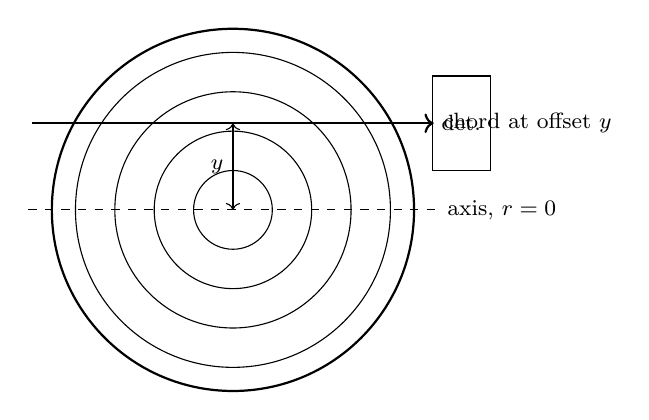
\begin{tikzpicture}[scale=1.0, every node/.style={font=\footnotesize}]
 \foreach \r in {0.5,1.0,1.5,2.0} {
 \draw[black,thin] (0,0) circle (\r);
 }
 \draw[black,thick] (0,0) circle (2.3);
 \draw[black,dashed] (-2.6,0) -- (2.6,0) node[right] {axis, $r=0$};
 \draw[black,thick,->] (-2.55,1.1) -- (2.55,1.1);
 \draw[black] (2.55,1.1) node[right] {chord at offset $y$};
 \draw[black,<->] (0,0) -- (0,1.1) node[midway,left] {$y$};
 \draw[black] (2.9,1.1) node[draw,rectangle,minimum width=0.4cm,minimum height=1.2cm] {det.};
\end{tikzpicture}
\caption{Schematic (illustrative, not measured) geometry for line-of-sight integration through a cylindrically symmetric emitting plasma column. A chord at perpendicular offset $y$ records the integral of Eq.~\eqref{eq:oes-los}; a set of such chords at different $y$ is required as input to the Abel inversion of Eq.~\eqref{eq:oes-abelinv}.}
\label{fig:oes-abel-schematic}
\end{figure}

\subsection{Representative diagnostic transitions}

Table~\ref{tab:oes-lines} lists, for orientation, representative upper-level energies and decay rates for transitions commonly exploited in argon and helium line-ratio and CR-model diagnostics. The values are illustrative, order-of-magnitude figures typical of the $4p\to4s$ argon manifold and the singlet/triplet helium system used throughout this chapter's cited works; they are not measurements from this work, nor a substitute for a validated atomic database.

\begin{table}[htbp]
\centering
\caption{Illustrative order-of-magnitude atomic parameters for representative visible transitions used in OES electron-temperature diagnostics. Values are indicative only, not experimental data from this work.}
\label{tab:oes-lines}
\begin{tabular}{@{}llcc@{}}
\toprule
Species & Transition class & Upper-level energy $E_{p}$ (\si{\eV}) & Decay rate $A_{p}$ (\si{\per\second}) \\
\midrule
Ar\,\textsc{i} & $4p\to4s$ manifold & $\sim 13$--$15$ & $\sim 10^{7}$--$10^{8}$ \\
He\,\textsc{i} & singlet ($3^{1}D\to2^{1}P$) & $\sim 23$ & $\sim 10^{7}$ \\
He\,\textsc{i} & triplet ($3^{3}D\to2^{3}P$) & $\sim 23$ & $\sim 10^{7}$ \\
Xe\,\textsc{i} & $6p\to6s$ manifold & $\sim 9$--$11$ & $\sim 10^{6}$--$10^{7}$ \\
\bottomrule
\end{tabular}
\end{table}

Figure~\ref{fig:oes-rate-curve} illustrates the strongly nonlinear sensitivity of a threshold-type excitation rate coefficient to $T_{\mathrm{e}}$ underlying the line-ratio sensitivity of Section~\ref{sec:oes-lineratio}, using the Arrhenius-type model of Eq.~\eqref{eq:oes-arrhenius} for two threshold energies.

\begin{figure}[htbp]
\centering
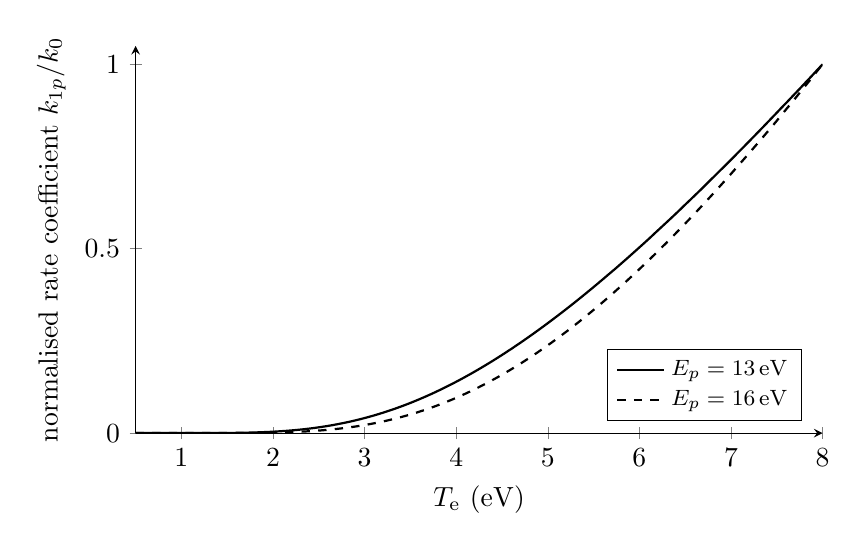
\begin{tikzpicture}
\begin{axis}[
 width=0.85\linewidth, height=6.5cm,
 xlabel={$T_{\mathrm{e}}$ (\si{\eV})},
 ylabel={normalised rate coefficient $k_{1p}/k_{0}$},
 domain=0.5:8, samples=120,
 xmin=0.5, xmax=8, ymin=0, ymax=1.05,
 axis lines=left,
 legend pos=south east,
 legend style={font=\footnotesize},
 every axis plot/.append style={thick, black},
]
\addplot[black, solid] {sqrt(x/8)*exp(-13/x)/ (sqrt(1)*exp(-13/8))};
\addlegendentry{$E_{p}=\SI{13}{\eV}$}
\addplot[black, dashed] {sqrt(x/8)*exp(-16/x)/ (sqrt(1)*exp(-16/8))};
\addlegendentry{$E_{p}=\SI{16}{\eV}$}
\end{axis}
\end{tikzpicture}
\caption{Schematic, analytic illustration (not measured data) of the strongly nonlinear dependence of a threshold-type Maxwellian-averaged excitation rate coefficient, Eq.~\eqref{eq:oes-arrhenius}, on $T_{\mathrm{e}}$, normalised to its value at $T_{\mathrm{e}}=\SI{8}{\eV}$, for two threshold energies $E_{p}$. The differential sensitivity between the curves is the physical basis of two-line electron-temperature thermometry.}
\label{fig:oes-rate-curve}
\end{figure}

\section{Strengths and Limitations}

\subsection{Strengths}

The passivity of OES translates into concrete practical advantages over material-probe diagnostics. Because no surface is inserted, there is no local perturbation of the sheath, the presheath field, or the ambient particle and energy fluxes — valuable when the goal, as here, is to characterise the very boundary layer a probe would otherwise disturb. There is no probe contamination or sputtering, no biasing or arcing risk in electronegative or high-density plasmas, and no restriction to plasmas accessible to a mechanically inserted tip, so OES functions equally well in high-density, high-power, or hazardous discharges (magnetron sources, Hall thrusters, atmospheric-pressure jets) where a Langmuir probe would be destroyed, draw prohibitive current, or be geometrically inaccessible. It is also remote and non-contact, compatible with real-time process monitoring and with energetic environments such as thruster exhaust plumes \cite{ref0256,ref0257} where material probes erode severely. Finally, because the same spectrum can, in favourable cases, simultaneously yield $T_{\mathrm{e}}$, $n_{\mathrm{e}}$, relative species densities (actinometry), gas temperature (molecular bands), and, via Doppler broadening, heavy-particle temperature, OES offers a rich, multi-parameter return on one minimally invasive measurement.

\subsection{Limitations}

These strengths are counterbalanced by real limitations. First, OES measures only what the plasma radiates and provides no direct measurement of the ion velocity distribution $f_{\mathrm{i}}(v)$, the ion flux, or the sheath potential profile — the central quantities of this monograph — which must come from complementary techniques combined with OES-derived $T_{\mathrm{e}}$ and $n_{\mathrm{e}}$. Second, accuracy is only as good as the CR model and cross-section database used in the inversion of Eq.~\eqref{eq:oes-chisq}; disagreements of tens of per cent against the Langmuir probe are not uncommon, traceable to incomplete cascade or metastable treatment, missing non-Maxwellian corrections, or outdated cross-section data — cross-comparison against an electrostatic-probe benchmark has repeatedly been used to quantify this \cite{ref0266}. Third, a chordal measurement without Abel inversion or tomography returns only an emissivity-weighted average, obscuring gradients expected across a thin presheath unless spatial resolution is engineered by narrow optics, translation scanning, or tomography. Fourth, the coronal-limit formulas that make OES tractable break down as $n_{\mathrm{e}}$ rises toward the regime where stepwise excitation and quenching become significant. Finally, actinometry assumes the admixed gas does not itself perturb the plasma chemistry at the concentration needed for adequate signal — an assumption that must be checked, not asserted, in reactive discharges.

\section{Role in the Multi-Diagnostic Fusion}

No single diagnostic treated here — Langmuir probe, laser-induced fluorescence, retarding-field energy analyser, or OES — is individually sufficient to constrain the full set of quantities entering the ion energy flux delivered across the plasma sheath,
\begin{equation}
\Gamma_{E} = \int q\,\phi_{\mathrm{tot}}(v)\, v\, f_{\mathrm{i}}(v)\, \mathrm{d}v ,
\label{eq:oes-gammae}
\end{equation}
where $\phi_{\mathrm{tot}}$ is the total energy (kinetic plus sheath acceleration) acquired by an ion of speed $v$ crossing the sheath, and $f_{\mathrm{i}}(v)$ is the ion velocity distribution at the sheath edge. Evaluating Eq.~\eqref{eq:oes-gammae}, or its Bohm-flux approximation $\Gamma_{E}\approx n_{\mathrm{e}} u_{\mathrm{B}} \langle E_{\mathrm{i}}\rangle$ with $u_{\mathrm{B}}=\sqrt{T_{\mathrm{e}}/M_{\mathrm{i}}}$ the Bohm velocity, requires $n_{\mathrm{e}}$ and $T_{\mathrm{e}}$ at the sheath edge, the sheath potential drop setting mean ion impact energy, and, for a fully kinetic treatment, the shape of $f_{\mathrm{i}}(v)$ itself. Within this book's diagnostic strategy, OES supplies the bulk-plasma or presheath-edge $n_{\mathrm{e}}$ and $T_{\mathrm{e}}$ that anchor the Bohm-velocity prefactor and, through the Debye length $\lambda_{\mathrm{D}} = \sqrt{\varepsilon_{0}T_{\mathrm{e}}/(n_{\mathrm{e}}e^{2})}$, the sheath thickness scale used throughout earlier chapters — supplied non-invasively, without the geometric and current-collection uncertainties of Langmuir-probe analysis. Laser-induced fluorescence and Doppler-resolved OES line widths independently constrain the ion temperature $T_{\mathrm{i}}$ and the ion velocity distribution's shape, cross-checking the Boltzmann or Maxwellian assumptions used to interpret OES line ratios. The retarding-field energy analyser and Langmuir probe supply direct in-situ measurements of the ion energy distribution and local floating and plasma potentials that OES cannot access, but at the cost of a physically inserted, current-collecting surface whose perturbation of the local sheath structure is exactly the quantity being measured. This cross-referencing is not merely a convenience: because each diagnostic is sensitive to a different moment or spatial region of the plasma, systematic comparison — OES against an electrostatic-probe benchmark \cite{ref0266} — is the principal available check on the accuracy of any single method, and standard practice wherever OES is deployed among several diagnostics characterising electric-propulsion discharges \cite{ref0256,ref0257} or industrial processing plasmas. The division of labour adopted here: OES furnishes the passively measured $n_{\mathrm{e}}(x)$ and $T_{\mathrm{e}}(x)$ profile feeding the Bohm-criterion boundary condition; Langmuir-probe and retarding-field-analyser data furnish the local potential structure and directly sampled ion energy distribution; and laser-induced-fluorescence Doppler measurements furnish an independent ion velocity distribution against which fluid-model closure assumptions can be tested. No measurement in this triad is redundant: each closes a different gap in the chain of inference to $\Gamma_{E}$ of Eq.~\eqref{eq:oes-gammae}, and only the combination yields an ion energy flux estimate whose uncertainty budget is fully closed.

\subsection{Summary}

Optical emission spectroscopy extracts $T_{\mathrm{e}}$ and $n_{\mathrm{e}}$ from the plasma's own light, exploiting the threshold-governed sensitivity of electron-impact excitation rate coefficients through two-line-ratio and actinometric methods, and, more rigorously, through inversion of a full collisional-radiative population balance spanning the coronal and LTE limits as special cases. Reliable quantitative use demands a validated cross-section database; careful wavelength and, where absolute intensities are required, radiometric calibration; explicit treatment of line-of-sight integration, via Abel inversion or tomography, whenever spatial resolution across a gradient region such as a presheath is required; and an honest accounting of errors from cascading, metastable pumping, self-absorption, and non-Maxwellian populations. Set against these demands are the technique's decisive practical virtues — passive, non-perturbing, remote, and compatible with plasma regimes inaccessible to material probes — which is why OES occupies a permanent place alongside the Langmuir probe, the retarding-field energy analyser, and laser-induced fluorescence in the multi-diagnostic strategy used here to constrain the electron-side boundary conditions, the Debye and sheath length scales, and, ultimately, the ion energy flux $\Gamma_{E}$ across the plasma sheath.

\chapter{Laser-Induced Fluorescence and the Ion Velocity Distribution}
\label{ch:lif}

The preceding chapters treat the ion energy flux delivered to a bounding surface,
\begin{equation}
\Gamma_{E} = \int \frac{1}{2} m_{\mathrm{i}} v^{2}\, v\, f_{\mathrm{i}}(v)\, \mathrm{d}v ,
\label{eq:lif-gammaE-def}
\end{equation}
as a functional of the ion velocity distribution function $f_{\mathrm{i}}(v)$ at, or just outside, the sheath edge. Every result derived elsewhere in this monograph -- the Bohm speed $u_{\mathrm{B}} = \sqrt{k_{\mathrm{B}} T_{\mathrm{e}}/m_{\mathrm{i}}}$, the presheath acceleration profile, the collisional broadening of the ion energy distribution in a radio-frequency sheath -- is a statement about the shape of $f_{\mathrm{i}}(v)$. This is a difficulty because $f_{\mathrm{i}}(v)$ is not an electrical signal: a Langmuir probe returns a current-voltage characteristic from which distribution moments emerge only after differentiation and strong assumptions, and any probe inserted into the sheath perturbs the object it measures. Laser-induced fluorescence (LIF) is the one diagnostic that returns the ion velocity distribution directly, non-invasively, with velocity-space resolution limited by the laser's linewidth rather than by an intrusive probe sheath. This chapter develops the principle of LIF, its Doppler-resolved variant for reconstructing $f_{\mathrm{i}}(v)$, its application to drift, temperature, and heating near sheaths, the systematic effects that must be controlled, the required apparatus, and why LIF is the key observable for quantifying ion energy flux across sheaths.

\section{The Physical Principle of Laser-Induced Fluorescence}

\subsection{Resonant excitation and spontaneous fluorescence}

LIF exploits the discrete spectrum of bound electronic states of an ion (or atom): a photon matching the separation between two states is resonantly absorbed, promoting the particle from a lower state $\lvert 1 \rangle$ to an upper state $\lvert 2 \rangle$. The excited population relaxes, in a mean radiative lifetime $\tau_{2} = 1/A_{21}$ set by the Einstein $A$-coefficient, by spontaneous emission near the same wavelength. Because excitation is resonant, only ions whose velocity component along the laser wavevector $\hat{\mathbf{k}}$ Doppler-shifts the transition into coincidence with $\nu_{L}$ are excited, and only the matching species responds. This selectivity, with nanosecond-scale, isotropic fluorescence emission, makes LIF simultaneously species-selective, velocity-resolved, and spatially localized to the beam-collection intersection volume \cite{ref0300,ref0292}.

A narrow-linewidth, tunable laser is directed through the plasma along $\hat{\mathbf{k}}$; fluorescence from the intersection volume is imaged onto a photodetector, typically through a narrow-band interference filter separating fluorescence from background plasma emission and stray laser light. As $\nu_{L}$ is scanned across resonance, the fluorescence intensity traces an excitation spectrum encoding the projection of the ion velocity distribution along $\hat{\mathbf{k}}$, broadened by the transition's intrinsic linewidth.

\subsection{Two-level excitation schemes}

The simplest scheme treats the ion as two levels: a lower state $\lvert 1 \rangle$, populated by electron-impact excitation or direct ionization, and an upper state $\lvert 2 \rangle$ connected by an electric-dipole transition at $\nu_{0} = (E_{2}-E_{1})/h$, with absorption and emission at the same wavelength. This is conceptually clean but has two drawbacks for ion diagnostics: reabsorption of the fluorescence photon by the dense ground- or metastable-state population (resonance trapping) can distort the lineshape near walls and sheaths, and laser light scattered from chamber surfaces at exactly the fluorescence wavelength is hard to discriminate from the weak signal, since no wavelength shift is available to filter on.

\subsection{Three-level (and multi-level) schemes for ions}

For this reason, essentially all quantitative ion LIF work uses a three-level (or multi-level) scheme \cite{ref0292}. A metastable lower level $\lvert 1 \rangle$, populated in the bulk by electron-impact excitation from the ion ground state, is pumped to an upper level $\lvert 2 \rangle$, which decays along several branches; the diagnostic collects fluorescence on a branch terminating on a third level $\lvert 3 \rangle$, at a wavelength well separated from the laser. Because pump and probe wavelengths differ, the fluorescence photon is easily isolated from scattered laser light and wall scattering. The price is a reduced quantum yield (only the branching fraction to $\lvert 3\rangle$ contributes) and the requirement that $\lvert 1 \rangle$ be populated at sufficient density -- satisfied for many noble-gas ions (Ar\textsuperscript{+}, Xe\textsuperscript{+}, Kr\textsuperscript{+}) common as propellants or process gases, whose metastables carry percent-level fractions of the total ion density. Table~\ref{tab:lif-schemes} summarizes the trade-offs.

\begin{table}[h]
\centering
\caption{Qualitative comparison of two-level and three-level LIF excitation schemes for ion diagnostics.}
\label{tab:lif-schemes}
\begin{tabularx}{\linewidth}{@{}lXX@{}}
\toprule
Property & Two-level scheme & Three-level scheme \\
\midrule
Pump/probe wavelength & Identical & Distinct \\
Stray-light rejection & Poor (no wavelength discrimination) & Strong (interference filter on probe line) \\
Resonance trapping & Significant at high metastable density & Reduced (probe line usually optically thin) \\
Fluorescence yield & Set by full branching to $\lvert 1\rangle$ & Reduced by branching fraction to $\lvert 3\rangle$ \\
Lower-level population requirement & Ground or metastable state & Populated metastable state \\
Typical use for ions & Rare & Standard practice \\
\bottomrule
\end{tabularx}
\end{table}

Representative pairs include the Ar\,\textsc{ii} scheme pumped near \SI{668.6}{\nano\meter} with fluorescence at \SI{442.7}{\nano\meter}, and the Xe\,\textsc{ii} scheme pumped near \SI{834.7}{\nano\meter} with fluorescence at \SI{541.9}{\nano\meter}; related schemes have been cross-validated across devices from Hall and gridded ion thrusters to helicon sources \cite{ref0304,ref0322}. These illustrate atomic-structure properties, not measurements performed for this monograph.

\section{Doppler-Resolved LIF and Reconstruction of the Ion Velocity Distribution Function}

\subsection{The Doppler link between frequency and velocity}

The diagnostic power of LIF for ion energetics rests on the non-relativistic Doppler shift. An ion moving with velocity component $v_{\parallel}$ along $\hat{\mathbf{k}}$ perceives the laboratory-frame frequency $\nu_{L}$ shifted, in its own rest frame, to
\begin{equation}
\nu' = \nu_{L}\left(1 - \frac{v_{\parallel}}{c}\right).
\label{eq:lif-doppler-basic}
\end{equation}
Resonance occurs when $\nu'$ coincides with the rest-frame transition frequency $\nu_{0}$, i.e.\ when
\begin{equation}
\nu_{L} = \nu_{0}\left(1 + \frac{v_{\parallel}}{c}\right) \quad \Longleftrightarrow \quad v_{\parallel} = c\,\frac{\nu_{L}-\nu_{0}}{\nu_{0}} = c\,\frac{\Delta\nu}{\nu_{0}}.
\label{eq:lif-doppler-map}
\end{equation}
Equation~\eqref{eq:lif-doppler-map} is the central relation in ion LIF: it maps laser detuning $\Delta\nu = \nu_{L}-\nu_{0}$ linearly onto the ion velocity component along the probe direction. For typical transition frequencies ($\nu_{0} \sim \SI{4e14}{\hertz}$--$\SI{6e14}{\hertz}$) and ion speeds of order the Bohm speed ($u_{\mathrm{B}} \sim \SI{1e3}{\meter\per\second}$--$\SI{1e4}{\meter\per\second}$), the Doppler shifts lie in the range of hundreds of megahertz to several tens of gigahertz -- resolvable with a tunable laser of megahertz-level linewidth, which is why LIF, unlike fixed-wavelength optical emission spectroscopy, genuinely resolves the velocity distribution rather than a Doppler-broadened linewidth \cite{ref0292,ref0347}.

\subsection{Line-of-sight projection and the excitation spectrum}

Because only the velocity component along $\hat{\mathbf{k}}$ enters Equation~\eqref{eq:lif-doppler-map}, a single-beam measurement does not recover the full distribution $f_{\mathrm{i}}(\mathbf{v})$, but its projection onto $\hat{\mathbf{k}}$,
\begin{equation}
f_{\mathrm{i}}(v_{\parallel}) = \iint f_{\mathrm{i}}(\mathbf{v})\, \mathrm{d}v_{\perp,1}\, \mathrm{d}v_{\perp,2}.
\label{eq:lif-projection}
\end{equation}
The measured excitation spectrum $S(\nu_{L})$ is the convolution of this projection with the intrinsic lineshape $g(\nu)$ (natural, pressure, and instrumental broadening combined):
\begin{equation}
S(\nu_{L}) \;\propto\; \int f_{\mathrm{i}}(v_{\parallel})\, g\!\left[\nu_{L} - \nu_{0}\left(1+\frac{v_{\parallel}}{c}\right)\right] \mathrm{d}v_{\parallel}.
\label{eq:lif-convolution}
\end{equation}
In essentially all low-temperature-plasma LIF work the Doppler width from ion thermal and drift motion vastly exceeds the intrinsic linewidth (a few to a few tens of megahertz, versus hundreds of megahertz to several gigahertz for \SI{0.1}{\electronvolt}-to-few-\si{\electronvolt} ions). In this Doppler-dominated limit $g(\nu)$ acts as a delta function, and Equation~\eqref{eq:lif-convolution} reduces to
\begin{equation}
S(\nu_{L}) \;\propto\; f_{\mathrm{i}}\!\left(v_{\parallel} = c\,\frac{\nu_{L}-\nu_{0}}{\nu_{0}}\right),
\label{eq:lif-doppler-limit}
\end{equation}
so the measured spectrum \emph{is}, up to the linear rescaling of Equation~\eqref{eq:lif-doppler-map}, the one-dimensional IVDF itself -- the formal justification for "LIF measures the IVDF" \cite{ref0347}. Otherwise Equation~\eqref{eq:lif-convolution} must be inverted, by deconvolution against a known lineshape or Bayesian inference.

\subsection{Moments of the IVDF: density, drift, and temperature}

Once $f_{\mathrm{i}}(v_{\parallel})$ is recovered from $S(\nu_{L})$, its low-order moments give the local ion density (relative; absolute calibration requires additional population and collection-efficiency information), drift velocity, and temperature along $\hat{\mathbf{k}}$:
\begin{align}
n_{\mathrm{i}} &\propto \int f_{\mathrm{i}}(v_{\parallel})\, \mathrm{d}v_{\parallel}, \label{eq:lif-mom0} \\
u_{\mathrm{d}} &= \frac{1}{n_{\mathrm{i}}}\int v_{\parallel}\, f_{\mathrm{i}}(v_{\parallel})\, \mathrm{d}v_{\parallel}, \label{eq:lif-mom1} \\
T_{\mathrm{i}} &= \frac{m_{\mathrm{i}}}{k_{\mathrm{B}} n_{\mathrm{i}}}\int (v_{\parallel}-u_{\mathrm{d}})^{2}\, f_{\mathrm{i}}(v_{\parallel})\, \mathrm{d}v_{\parallel}. \label{eq:lif-mom2}
\end{align}
For a locally Maxwellian population drifting at $u_{\mathrm{d}}$,
\begin{equation}
f_{\mathrm{i}}(v_{\parallel}) \propto \exp\!\left[-\frac{m_{\mathrm{i}}(v_{\parallel}-u_{\mathrm{d}})^{2}}{2 k_{\mathrm{B}} T_{\mathrm{i}}}\right],
\label{eq:lif-maxwellian}
\end{equation}
the spectrum is a Gaussian centered at offset $\Delta\nu_{\mathrm{d}} = \nu_{0} u_{\mathrm{d}}/c$, with full width at half maximum
\begin{equation}
\Delta\nu_{\mathrm{D}} = \frac{\nu_{0}}{c}\sqrt{\frac{8 \ln 2\, k_{\mathrm{B}} T_{\mathrm{i}}}{m_{\mathrm{i}}}}.
\label{eq:lif-dopplerwidth}
\end{equation}
A fitted Gaussian width yields $T_{\mathrm{i}}$ directly via Equation~\eqref{eq:lif-dopplerwidth}, and the centroid yields $u_{\mathrm{d}}$ via Equation~\eqref{eq:lif-doppler-map}. The moment definitions apply to any measured $f_{\mathrm{i}}(v_{\parallel})$; the Gaussian fit is just the convenient near-equilibrium case. Near a sheath, where the distribution develops a beam-like high-velocity tail on a cooler bulk, the raw moments or full lineshape must be reported and compared with kinetic theory rather than compressed into a single temperature \cite{ref0338}.

Figure~\ref{fig:lif-doppler-schematic} illustrates the qualitative effect of a superposed bulk drift: an unshifted, narrower Gaussian for a stationary bulk population versus a shifted, broader Gaussian for an accelerated, heated population deeper in a presheath or sheath. Both curves are explicit analytic Gaussians for illustration only, not measured spectra.

\begin{figure}[h]
\centering
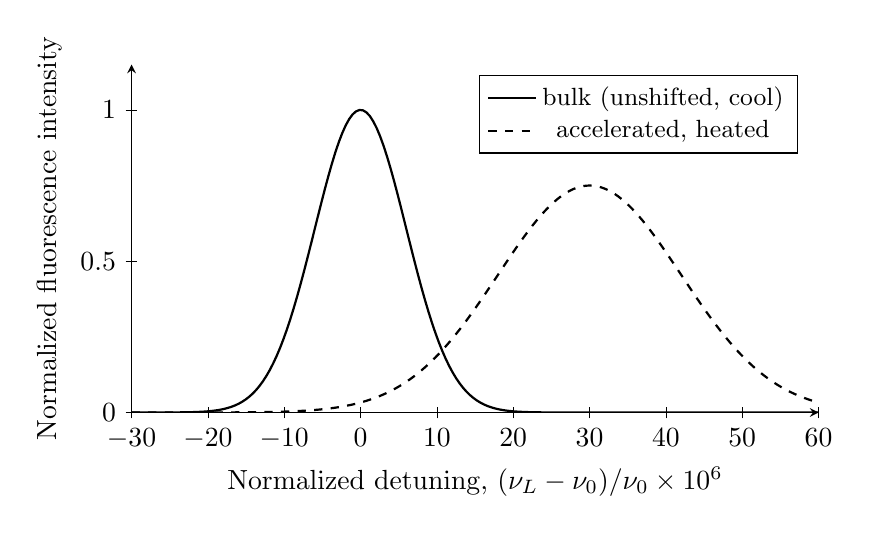
\begin{tikzpicture}
\begin{axis}[
 width=0.85\linewidth,
 height=6cm,
 xlabel={Normalized detuning, $(\nu_L-\nu_0)/\nu_0 \times 10^{6}$},
 ylabel={Normalized fluorescence intensity},
 xmin=-30, xmax=60,
 ymin=0, ymax=1.15,
 domain=-30:60,
 samples=200,
 axis lines=left,
 tick style={black},
 every axis plot/.append style={thick, black},
 legend style={draw=black, fill=white, font=\small},
 legend pos=north east,
]
\addplot[black, solid] {exp(-((x-0)^2)/(2*6^2))};
\addlegendentry{bulk (unshifted, cool)}
\addplot[black, dashed] {0.75*exp(-((x-30)^2)/(2*12^2))};
\addlegendentry{accelerated, heated}
\end{axis}
\end{tikzpicture}
\caption{Schematic, illustrative LIF excitation spectra for a stationary/cool bulk ion population (solid, narrow Gaussian at zero detuning) and a drifting/heated population near a sheath (dashed, shifted centroid and larger width). These are analytic Gaussians illustrating how drift and temperature map onto centroid and width; they are not measured or simulated data.}
\label{fig:lif-doppler-schematic}
\end{figure}

\subsection{From one dimension to three: multi-view and tomographic reconstruction}

A single-beam measurement returns only the projection of $f_{\mathrm{i}}(\mathbf{v})$ along one direction. Full characterization of an anisotropic distribution -- essential near a sheath, where the distribution is compressed and accelerated preferentially along the sheath normal while remaining comparatively unperturbed transversely -- requires either an assumption of separability (transverse components stay Maxwellian at bulk temperature while the parallel component is measured directly) or genuinely multi-view measurements: repeating the measurement along two or three non-collinear directions at the same point to extract drift and temperature components from independent projections \cite{ref0347}, or planar/volumetric LIF, which expands the beam into a sheet or scans it across a plane and images fluorescence with a two-dimensional (intensified or gated CCD) detector, obtaining spatially resolved velocity-space information over an extended region simultaneously \cite{ref0304}. Tomographic extensions, combining multiple views via inverse Radon-type reconstruction, have recovered three-dimensional IVDFs in electric-thruster exhaust plumes, where the flow is neither one-dimensional nor azimuthally simple \cite{ref0328}. Spatially resolved single-line-of-sight scans across a boundary layer remain the workhorse for sheath studies, since the dominant physics -- acceleration along the sheath normal -- is well captured by a one-dimensional projection aligned with that normal.

\section{Measuring Drift, Temperature, and Heating Near and Within Sheaths}

\subsection{The presheath-to-sheath transition in velocity space}

LIF measurements confirm that the ion velocity distribution evolves continuously, with distinct signatures, across three zones: the quasineutral bulk, close to Maxwellian with a drift set by whatever bulk flow or ambipolar field is present; the presheath, where a weak field accelerates ions over a distance of order the ion-neutral mean free path or device dimension, shifting the centroid of $f_{\mathrm{i}}(v_{\parallel})$ toward higher velocity while, in a collisionless source-free presheath, leaving its shape close to a shifted Maxwellian; and the sheath itself, a few Debye lengths $\lambda_{\mathrm{D}}$ thick, where the field strengthens by orders of magnitude and ions accelerate essentially ballistically, compressing the distribution in velocity space as flux-conserving acceleration outruns local thermalization. Because $\Gamma_{E}$ (Equation~\eqref{eq:lif-gammaE-def}) depends on the third velocity moment, it is disproportionately sensitive to the high-velocity tail, and LIF alone resolves that tail directly rather than inferring it from a fluid closure. A spatially scanned measurement translated from bulk through presheath to sheath records this evolution: $u_{\mathrm{d}}(x)$, via Equation~\eqref{eq:lif-mom1}, rises monotonically toward the boundary, approaching and exceeding the Bohm speed at the nominal sheath edge, while the distribution width -- and effective parallel temperature -- either narrows (acceleration outpacing competing heating) or broadens (collisions, instabilities, or a non-monotonic presheath field) \cite{ref0329}.

The earliest and still most direct demonstrations recorded the IVDF versus position across a well-characterized sheath boundary, observing smooth acceleration of the centroid and departures from a shifted-Maxwellian shape near the sheath edge \cite{ref0329}. Subsequent work extended the measurement to two-dimensional distributions above radio-frequency-biased electrodes, resolving normal and transverse components simultaneously. Because ion transit time across the sheath is typically comparable to or shorter than a radio-frequency period, phase-resolved LIF -- synchronizing the probe to a fixed drive phase and repeating across successive phases to build a movie of the evolving distribution -- has proven essential for characterizing ion energetics under a modulated sheath potential.

\subsection{Spatially and temporally resolved measurements}

LIF has also tracked transient sheath dynamics: the ion population's response to a fast disruption of discharge current, and the ionization oscillations intrinsic to Hall-thruster operation. Time-resolved measurements synchronized to a current disruption show the IVDF near the acceleration-channel exit responding on the ion transit timescale rather than instantaneously -- information only a diagnostic with sub-microsecond time resolution and direct velocity sensitivity can extract. Phase-resolved LIF has similarly characterized ion dynamics tied to the low-frequency "breathing mode" oscillations that dominate Hall thruster discharges, revealing periodic modulation of drift velocity and distribution width with oscillation phase. The general principle: whenever the sheath potential varies on a timescale comparable to or faster than the ion transit time, a time-averaged diagnostic (e.g.\ an ungated retarding-field analyzer) reports only time-averaged energetics, whereas LIF, given sufficient signal-to-noise at each phase, resolves the full time-dependent evolution of $f_{\mathrm{i}}(v_{\parallel})$ that determines the instantaneous, and hence time-averaged, energy flux.

\subsection{Non-Maxwellian features, beams, and heating signatures}

The measured IVDF frequently departs from the single shifted-Maxwellian form assumed by simple fluid models, in two common ways. The first is a distinct, faster secondary population -- a beam -- superposed on a slower bulk component, interpreted either as ions accelerated by a localized field structure (an electrostatic double layer or ion-acoustic shock) or as ions that underwent a charge-exchange or ionization event within the sheath or presheath and so carry a different velocity history; such populations have been directly observed in expanding helicon-source plasmas and shock-wave experiments, with the spectrum developing a clearly resolved second peak or shoulder. The second is excess broadening beyond what the local electron or neutral temperature predicts, interpreted as ion heating by wave-particle interactions, instabilities, or turbulent fields localized to the presheath-sheath transition. In both cases the diagnostic value of LIF is its ability to resolve shape rather than a single width: a fluid-model temperature force-fit to a genuinely bimodal or skewed distribution can systematically mislead a prediction of $\Gamma_{E}$, since the third-moment energy flux is sensitive to exactly the tail structure such a fit discards.

\section{Saturation, Quenching, Zeeman/Stark Effects, and Calibration}

Quantitative use of LIF requires that the measured spectrum be a faithful, linear representation of the underlying IVDF. Several physical effects can distort that representation if left uncontrolled.

\subsection{Optical saturation and rate-equation description}

At sufficiently high laser intensity the excitation-emission cycle no longer responds linearly: population is driven so strongly out of $\lvert 1 \rangle$ that further power increases produce diminishing fluorescence gains, and the measured lineshape itself distorts. This follows from the steady-state upper-state population fraction $\rho_{22}$ as a function of detuning $\delta = 2\pi(\nu_{L}-\nu_{0})$ and on-resonance Rabi frequency $\Omega$:
\begin{equation}
\rho_{22}(\delta) = \frac{\Omega^{2}/4}{\delta^{2} + \Gamma^{2}/4\,(1+S_{0})} , \qquad S_{0} \equiv \frac{\Omega^{2}/2}{\Gamma^{2}/4} = \frac{I}{I_{\mathrm{sat}}},
\label{eq:lif-saturation}
\end{equation}
where $\Gamma$ is the natural linewidth (angular frequency), $I$ the local laser intensity, and $I_{\mathrm{sat}}$ the saturation intensity. Equation~\eqref{eq:lif-saturation} shows two consequences of $S_{0} \gtrsim 1$: the signal saturates (grows sublinearly with $I$, so absolute density calibration becomes unreliable), and the linewidth power-broadens by $\sqrt{1+S_{0}}$, inflating the apparent temperature via Equation~\eqref{eq:lif-dopplerwidth}. Because real beams have a finite, roughly Gaussian, spatial profile, different velocity classes at different transverse positions experience different $S_{0}$, so spatially inhomogeneous saturation can asymmetrically distort the lineshape even at modest peak intensities. This is especially consequential near reflecting surfaces -- the sheath-adjacent geometry of greatest interest -- where multiply reflected light can locally re-saturate the transition and bias the distribution inferred near the wall. Best practice is a power scan (extrapolating fitted centroid and width to zero power) or verified operation at a low $S_{0}$ established from independent characterization of $I_{\mathrm{sat}}$ and beam profile.

\subsection{Collisional quenching of the upper level}

Population reaching $\lvert 2 \rangle$ competes between radiative decay (rate $A_{21}$) and non-radiative, collisional de-excitation by background neutrals, electrons, or ions (rate $Q$, proportional to quenching-partner density and cross section). The fluorescence quantum yield is
\begin{equation}
\eta = \frac{A_{21}}{A_{21}+Q},
\label{eq:lif-quenching}
\end{equation}
and quenching reduces the absolute signal without distorting its shape, provided the quenching rate is uniform across the probed velocity classes and volume. Quenching concerns absolute density calibration and LIF at elevated neutral pressure (a dense presheath, or higher-pressure processing discharges), where $Q$ can approach or exceed $A_{21}$ for metastable-to-resonance transitions with tens-of-nanosecond lifetimes. Because $\eta$ depends on local neutral density, which varies across the presheath-sheath transition from sputtering products, outgassing, or pressure gradients, uncorrected quenching variation can masquerade as an ion-density variation; quantitative studies therefore report an independently characterized quenching correction, or restrict interpretation to shape rather than absolute normalization, which is unaffected by a spatially uniform $\eta$.

\subsection{Zeeman and Stark perturbations of the lineshape}

Two further effects matter near sheaths and in magnetized devices. In a magnetized plasma (relevant to Hall thrusters and sheaths at oblique field lines), the field $B$ splits each fine-structure level into $2J+1$ sublevels separated by an amount proportional to $B$ and the Land\'e $g$-factor. If this splitting is not small compared with the Doppler width, the measured lineshape is a superposition of shifted, differently weighted Zeeman components rather than a single Doppler profile, and naive single-Gaussian fitting biases the inferred temperature and can introduce a spurious drift. Quantitative treatments model the full Zeeman pattern, including polarization dependence, or choose a viewing geometry (typically along $\mathbf{B}$, collecting only symmetric $\sigma$-components) that minimizes distortion.

The Stark effect -- shift and splitting of levels by a local field -- matters inside the sheath, where field strength can reach $\SI{e5}{\volt\per\meter}$ to $\SI{e7}{\volt\per\meter}$ depending on sheath thickness and bias. For hydrogenic structures the shift is linear in field strength; for the non-hydrogenic transitions used in three-level LIF it is quadratic and typically smaller, but not negligible at the highest fields deep inside a strongly biased sheath. Because the Stark shift, unlike the Doppler shift, does not depend on velocity, an uncorrected Stark shift manifests as an apparent field-dependent centroid offset that could be misattributed to anomalously large drift. Good practice restricts quantitative determination of $u_{\mathrm{d}}(x)$ and $T_{\mathrm{i}}(x)$ to regions with independently characterized field, or incorporates a field-dependent correction into the lineshape model.

\subsection{Frequency and velocity calibration}

Because Equation~\eqref{eq:lif-doppler-map} converts frequency detuning into velocity via division by $\nu_{0}$, accurate determination requires an absolute frequency reference for the scanning laser: (i) mapping the laser tuning onto an absolute frequency scale, typically with a scanning Fabry-P\'erot etalon for relative markers plus a saturated-absorption cell or wavemeter for the absolute origin; and (ii) establishing the zero-velocity point of the spectrum, from a low-drift reference population or the known $\nu_{0}$ itself. Systematic frequency-calibration errors translate linearly into drift-velocity errors and hence into $\Gamma_{E}$; since $\Gamma_{E}$ scales as $v^{3}$, a modest fractional velocity-calibration error is amplified in the inferred energy flux, motivating careful, redundant calibration. Modern implementations increasingly lock fluorescence acquisition to the instantaneous, independently monitored laser frequency shot-by-shot, reducing uncertainty from frequency jitter between scan points. Table~\ref{tab:lif-errors} summarizes the principal error sources and their mitigation.

\begin{table}[h]
\centering
\caption{Principal systematic error sources in quantitative ion LIF and their standard mitigation.}
\label{tab:lif-errors}
\begin{tabularx}{\linewidth}{@{}lX@{}}
\toprule
Effect & Standard mitigation \\
\midrule
Optical saturation & Power scan and extrapolation to zero laser intensity; verified operation at $S_{0}\ll 1$ \\
Spatially inhomogeneous saturation & Careful beam profiling; avoidance of near-wall multiple reflections \\
Collisional quenching & Independent characterization of local neutral density; restrict interpretation to lineshape rather than absolute intensity \\
Zeeman splitting & Viewing along $\mathbf{B}$; explicit multi-component fit including known Land\'e factors \\
Stark shift/broadening & Restriction to regions of characterized field strength; field-dependent lineshape model where needed \\
Frequency calibration & Fabry-P\'erot etalon markers; saturated-absorption or wavemeter reference; synchronized digital acquisition \\
\bottomrule
\end{tabularx}
\end{table}

\section{Apparatus: Tunable Lasers, Optical Access, Detection, and Signal Recovery}

\subsection{Tunable narrow-linewidth lasers}

Ion LIF requires a continuously tunable, single-longitudinal-mode laser with linewidth small compared with the Doppler width (well under \SI{10}{\mega\hertz}), sufficient mode-hop-free tuning range to scan the full Doppler-shifted lineshape (a few gigahertz), and enough optical power, after transmission losses, to achieve adequate signal-to-noise without approaching saturation. External-cavity diode lasers, and earlier continuous-wave dye or Ti:sapphire lasers, have supplied these requirements at the near-infrared/visible wavelengths of the common Ar\,\textsc{ii}, Xe\,\textsc{ii}, and Kr\,\textsc{ii} pump transitions; diode-laser systems are now standard for their compactness, mode-hop-free piezo tuning, and low cost, enabling deployment on laboratory and flight-representative thruster test stands.

\subsection{Optical access and beam/collection geometry}

Because LIF requires simultaneous beam injection and fluorescence collection from a well-defined intersection volume, the chamber must provide at least two, typically three or more, optical ports: one or more for laser injection, and one -- most commonly at $90^{\circ}$ to the beam -- for fluorescence collection. Anti-reflection-coated, vacuum-compatible viewports are standard; stray reflections from viewports and walls are a persistent source of both optical background and localized saturation, so substantial design effort goes into beam dumps and baffling near walls or electrodes. Spatial resolution is set by the smaller of the beam waist and the collection optics' depth of field; typical implementations achieve millimeter-scale resolution, sufficient for the presheath but marginal for a collisionless sheath only a few Debye lengths thick, motivating specialized confocal or ring-beam geometries.

\subsection{Detectors and background rejection}

The fluorescence flux is typically orders of magnitude weaker than ambient plasma emission and stray laser light, so detector choice and background rejection are central. Photomultiplier tubes, chosen for high quantum efficiency and low dark count, remain the standard single-point detector, coupled through fiber or free-space optics and a narrow-band interference filter (roughly \SI{1}{\nano\meter} to a few nanometers bandpass) rejecting the pump wavelength and continuum emission. For imaging implementations, intensified or electron-multiplying CCD cameras, gated synchronously with a pulsed laser, add spatial resolution while rejecting background temporally by restricting exposure to a narrow window around each pulse \cite{ref0304}.

\subsection{Modulation, lock-in, boxcar, and phase-resolved acquisition}

Residual background leaking through the interference filter is often comparable to or larger than the fluorescence signal, particularly in a bright discharge or near an emissive wall. The standard solution modulates the laser -- mechanical chopping or drive-current modulation -- at a frequency (hundreds of hertz to tens of kilohertz) away from characteristic plasma fluctuations, and demodulates with a lock-in amplifier referenced to that frequency. Because only fluorescence correlates with the modulation, this synchronous detection rejects unmodulated background essentially completely, improving signal-to-noise by orders of magnitude and enabling quantitative LIF even in bright, high-density discharges \cite{ref0292}. For pulsed lasers, boxcar integration -- gating detection to a narrow window after each pulse -- serves the same purpose. Where the sheath potential varies periodically, gating must also be referenced to a fixed drive phase, so the spectrum corresponds to a single instant rather than a cycle-averaged blur; phase-resolved acquisition across a sequence of phases spanning the drive period is the standard approach for reconstructing the time-dependent IVDF across a radio-frequency sheath cycle.

\subsection{Planar and tomographic LIF imaging}

Point-by-point translation is adequate for steady, one-dimensional boundary-layer structure but is laborious, and potentially unreliable amid shot-to-shot drift, when a two- or three-dimensional map is needed. Planar LIF expands the laser into a thin sheet and images the fluorescence plane onto a gated camera, so an entire spatial slice is interrogated at a single frequency setting; repeating across frequency steps builds up, pixel by pixel, the spatially resolved $f_{\mathrm{i}}(v_{\parallel})$ far faster than sequential points \cite{ref0304}. Combining multiple such views at different angles, tomographic reconstruction recovers a genuinely three-dimensional IVDF, demonstrated in an electric thruster's exhaust plume where flow is not reducible to a single direction \cite{ref0328}. These variants trade increased apparatus complexity, cost, and laser power for substantially greater spatial and temporal coverage, and are increasingly the method of choice for non-planar sheath and presheath geometries.

\section{Why LIF Is the Key Observable for Ion Energetics}

\subsection{From the full distribution to the energy flux}

The primacy of LIF among sheath diagnostics is structural, not merely a matter of precision: $\Gamma_{E}$ (Equation~\eqref{eq:lif-gammaE-def}), and related quantities such as the ion energy distribution function delivered to a surface, are functionals of the full distribution $f_{\mathrm{i}}(v)$, weighted by $v^{3}$. Any diagnostic reporting only a subset of moments -- a Langmuir probe, returning at best a model-dependent ion-flux estimate via ion saturation current, or optical emission spectroscopy, returning line-integrated excited-state information rather than velocity-resolved population -- must supply the missing shape from an assumed functional form, typically a shifted Maxwellian. Because the $v^{3}$ weighting makes $\Gamma_{E}$ disproportionately sensitive to exactly the high-velocity tail that a parametric fit is least able to constrain, systematic non-Maxwellian structure -- a beam, a shock-accelerated population, a heated tail -- propagates into an amplified, uncontrolled error in a moment-based estimate. LIF sidesteps this: returning $f_{\mathrm{i}}(v_{\parallel})$ itself, essentially unfiltered by any assumed functional form (subject only to the caveats of Section~4), so $\Gamma_{E}$ can be evaluated by direct numerical integration via Equation~\eqref{eq:lif-gammaE-def}, without any parametric ansatz \cite{ref0338,ref0347}.

\subsection{Non-invasiveness and validation of other diagnostics}

A second reason for LIF's importance is its non-invasive character. Every electrical probe -- Langmuir probes, retarding-field analyzers, emissive probes -- inserts a solid, biased or floating object that forms its own local sheath and perturbs the ambient field and particle balance nearby; this is worst exactly where the information is most valuable, within a few Debye lengths of an existing boundary. LIF instead uses a beam of photons: it does not perturb the local field, collect or emit charge, or modify the population balance beyond promoting a small, controlled fraction to an excited state decaying on a nanosecond timescale, negligible against any transport timescale of interest. This makes LIF uniquely suited to measurements within, or immediately adjacent to, an existing sheath -- precisely where probe measurements are least trustworthy -- and the diagnostic of choice for validating the boundary conditions and closure assumptions used in the sheath theories developed elsewhere in this monograph. Comparisons between LIF-measured IVDFs and probe-inferred populations have repeatedly calibrated probe-based methods and identified regimes where probe-based inference breaks down \cite{ref0329}.

\subsection{Coverage across sheath-relevant applications}

The breadth of systems to which ion LIF has been applied evidences its centrality: the acceleration channel and near-plume region of Hall-effect thrusters, where the local IVDF determines thrust efficiency and the erosion-driving energy of ions bombarding channel walls \cite{ref0322}; gridded ion thrusters, resolving azimuthal and axial velocity components in the accelerated beam; helicon and electron-cyclotron-resonance sources, measuring parallel ion flow versus discharge power and magnetic configuration; and reconnection and sputtering studies, diagnosing energy conversion and sputtered-flux energetics. This breadth establishes LIF not as one diagnostic option among several of comparable standing, but as the reference technique against which fluid and kinetic sheath models, and every other diagnostic of ion energetics, must ultimately be validated.

\section{Summary}

Laser-induced fluorescence provides the one direct, non-invasive, velocity-resolved measurement of the ion population underlying ion energy flux across a plasma sheath. Resonant absorption on a metastable-to-excited transition, followed by fluorescence collected on a spectrally separated probe line in the standard three-level architecture, converts the Doppler shift of ions moving along the laser wavevector into a directly measurable excitation spectrum; in the Doppler-dominated regime of essentially all low-temperature-plasma applications, this spectrum is, after linear rescaling, the ion velocity distribution function itself. Spatially and, where the sheath potential is time-varying, phase-resolved application traces drift velocity and effective temperature from the quasineutral bulk, through the presheath, to the sheath edge, while directly revealing non-Maxwellian structure -- beams, shock-accelerated populations, heating signatures -- that fluid closures cannot self-consistently predict. Quantitative use requires control of optical saturation, collisional quenching, Zeeman and Stark perturbations, and careful frequency and velocity calibration, each with an established mitigation strategy. The required apparatus -- a narrow-linewidth tunable laser, adequate optical access, a sensitive background-rejecting detection chain, and, where needed, phase-locked signal recovery -- is demanding but within reach of a dedicated laboratory, and planar/tomographic extensions extend coverage to multi-dimensional sheath geometries. Because ion energy flux is a $v^{3}$-weighted functional of the full IVDF, and LIF alone returns that distribution directly rather than through parametric or moment-based inference, laser-induced fluorescence stands as the key experimental observable for quantifying ion energy flux across plasma sheaths, and the essential empirical anchor for the treatments in the remaining chapters.

\chapter{Thomson Scattering}
\label{ch:thomson}

Of all the diagnostics surveyed in this monograph, laser Thomson scattering occupies a singular position: it measures the electron population of a plasma through a scattering process whose cross section is fixed by fundamental electrodynamics, not by an assumed collection model, collisional-radiative balance, or sheath structure. A photon of known wavelength and polarization is fired into the plasma; a small fraction of the incident photons are scattered by free electrons, and the Doppler-shifted, intensity-scaled spectrum of the scattered light encodes $T_{\mathrm{e}}$ and $n_{\mathrm{e}}$ directly, without the probe-sheath models that complicate Langmuir-probe inversion or the rate coefficients that complicate optical emission spectroscopy. This chapter develops the scattering physics, distinguishes the incoherent and coherent regimes, derives the working relations for $T_{\mathrm{e}}$ and $n_{\mathrm{e}}$, surveys the instrumentation needed to extract a vanishingly weak signal from an overwhelming stray-light background, and discusses attainable resolution — closing by situating Thomson scattering within the diagnostic hierarchy of this monograph as the direct, model-light anchor against which more accessible, more perturbative, or more model-dependent techniques are validated as the framework scales toward reactor- and thruster-relevant plasmas.

\section{Scattering of Light by Free Electrons}

\subsection{The Classical Scattering Cross Section}

Thomson scattering is the elastic (in the scatterer's rest frame) scattering of an electromagnetic wave by a free charge: an incident plane wave drives the electron through the Lorentz force, producing an oscillating acceleration that radiates a scattered wave at the same frequency, shifted only by the electron's own motion. For non-relativistic electron and quiver velocities, the differential cross section for scattering into solid angle $\mathrm{d}\Omega$ is
\begin{equation}
\frac{\mathrm{d}\sigma}{\mathrm{d}\Omega} = r_{\mathrm{e}}^{2}\sin^{2}\chi ,
\qquad
r_{\mathrm{e}} = \frac{e^{2}}{4\pi\varepsilon_{0} m_{\mathrm{e}} c^{2}} \approx \SI{2.818e-15}{\meter},
\label{eq:thomson-diff-xsec}
\end{equation}
where $r_{\mathrm{e}}$ is the classical electron radius and $\chi$ the angle between the observation direction and the driven-dipole polarization. Integrating over solid angle gives the total Thomson cross section,
\begin{equation}
\sigma_{\mathrm{T}} = \frac{8\pi}{3} r_{\mathrm{e}}^{2} \approx \SI{6.652e-29}{\meter\squared}.
\label{eq:thomson-total-xsec}
\end{equation}
This cross section is a fixed constant of nature, independent of plasma conditions; it requires no calibration against a boundary-layer model and depends on no excited-state populations, quenching rates, or assumed distribution shape. This is why the technique is described throughout as \emph{model-light}: the only physics standing between the measured photon spectrum and $T_{\mathrm{e}}$, $n_{\mathrm{e}}$ is single-particle (or, in the coherent regime, collective) electrodynamics, known to very high precision.

Because $\sigma_{\mathrm{T}} \propto m_{\mathrm{e}}^{-2}$, scattering from ions is suppressed relative to electrons by $(m_{\mathrm{e}}/m_{\mathrm{i}})^{2}$, typically $10^{-8}$ or smaller, making free-electron Thomson scattering an electron diagnostic \emph{by construction}: information about $T_{\mathrm{i}}$, $n_{\mathrm{i}}$, or $f_{\mathrm{i}}(v)$ enters only indirectly, through electron-density fluctuations organized by ion dynamics in the coherent regime — complementing laser-induced fluorescence, which probes $f_{\mathrm{i}}(v)$ via a resonant transition.

At sufficiently high incident intensity, the electron quiver velocity becomes a non-negligible fraction of $c$, and relativistic corrections to the cross section and ponderomotive force must be included; particle-in-cell studies have quantified the onset of such perturbations \cite{ref0360}. These effects are small at fluences typical of low-temperature and edge-plasma systems, but they bound how aggressively laser energy can be raised to compensate for weak signal in low-density plasmas, a tension revisited in Section~\ref{sec:low-density-challenge}.

\subsection{Incoherent versus Coherent Regimes: The Scattering Parameter}

The character of the scattered spectrum depends on whether it probes individual, uncorrelated electrons or collective density fluctuations organized by Debye screening. The relevant wavevector is the scattering vector,
\begin{equation}
\mathbf{k} = \mathbf{k}_{\mathrm{s}} - \mathbf{k}_{\mathrm{i}}, \qquad
k = |\mathbf{k}| = \frac{4\pi}{\lambda_{0}}\sin\!\left(\frac{\theta}{2}\right),
\label{eq:scattering-vector}
\end{equation}
where $\lambda_{0}$ is the incident laser wavelength, $\theta$ the scattering angle, and $|\mathbf{k}_{\mathrm{s}}|\approx|\mathbf{k}_{\mathrm{i}}|$ since the fractional frequency shift is minute. Whether the scattered light samples individual trajectories or the collective response is governed by the dimensionless \emph{scattering parameter}
\begin{equation}
\alpha \equiv \frac{1}{k\lambda_{\mathrm{D}}}
= \frac{\lambda_{0}}{4\pi\lambda_{\mathrm{D}}\sin(\theta/2)},
\qquad
\lambda_{\mathrm{D}} = \sqrt{\frac{\varepsilon_{0} T_{\mathrm{e}}}{n_{\mathrm{e}} e^{2}}},
\label{eq:scattering-parameter}
\end{equation}
where $\lambda_{\mathrm{D}}$ is the electron Debye length (temperatures in energy units throughout). Physically, $\alpha$ compares the probed spatial scale $k^{-1}$ to the Debye length: for $\alpha\ll1$ the probe wavelength is too short to resolve collective screening and each electron scatters independently; for $\alpha\gg1$ the probed scale exceeds the screening cloud and the light responds to collective fluctuations — Debye shielding, ion-acoustic waves, Langmuir oscillations.

\paragraph{Incoherent regime ($\alpha \ll 1$).} Most laser and low-temperature plasma Thomson systems, at visible wavelengths and moderate-to-large scattering angles, fall into or near this regime for typical processing- and thruster-plasma densities. The scattered spectrum reproduces the projection of the electron velocity distribution onto the scattering direction, and its width yields $T_{\mathrm{e}}$ directly, as derived in Section~\ref{sec:te-derivation}.

\paragraph{Coherent regime ($\alpha \gg 1$).} A small scattering angle, or a dense, cold plasma, moves a system into the coherent regime, where the scattered spectrum develops two satellite families: high-frequency \emph{electron feature} satellites near $\omega_{\mathrm{pe}}$, and low-frequency \emph{ion feature} satellites near the ion-acoustic frequency $k c_{\mathrm{s}}$, with $c_{\mathrm{s}} = \sqrt{(Z T_{\mathrm{e}} + 3T_{\mathrm{i}})/m_{\mathrm{i}}}$. Because $c_{\mathrm{s}}$ is, up to numerical coefficients, the same combination as the Bohm velocity $u_{\mathrm{B}} = \sqrt{T_{\mathrm{e}}/m_{\mathrm{i}}}$ governing ion entry into the sheath throughout this monograph, collective Thomson scattering offers an independent route to $T_{\mathrm{i}}$, effective charge state $Z$, and bulk ion drift velocity, without an ion-resonant transition of the kind exploited by laser-induced fluorescence. Bayesian inference has been applied to extract these parameters from collective-regime spectra on gas-puff plasma sources \cite{ref0684}.

Table~\ref{tab:regimes} summarizes, schematically, the distinguishing features of the two regimes.

\begin{table}[htbp]
\centering
\caption{Illustrative overview of the incoherent and coherent Thomson scattering regimes, distinguished by the scattering parameter $\alpha$. This is a conceptual summary, not a set of measured values.}
\label{tab:regimes}
\begin{tabularx}{\linewidth}{@{}l X X@{}}
\toprule
Property & Incoherent regime ($\alpha \ll 1$) & Coherent regime ($\alpha \gg 1$) \\
\midrule
Physical picture & Independent single-electron scattering & Collective electron density fluctuations, Debye-screened \\
Spectral shape & Single Doppler-broadened line centered on $\lambda_0$ & Electron-feature and ion-feature satellite structure \\
Primary observable & Spectral width $\rightarrow T_{\mathrm{e}}$; integrated intensity $\rightarrow n_{\mathrm{e}}$ & Satellite spacing/shape $\rightarrow T_{\mathrm{i}}$, $Z$, drift velocity \\
Typical geometry & Moderate-to-large scattering angle & Small scattering angle or long probe wavelength \\
Representative applications & Edge/core profiles, processing and thruster plasmas & Magnetic mirrors, dense/warm dense plasmas, burning plasmas \\
\bottomrule
\end{tabularx}
\end{table}

\section{Extraction of Plasma Parameters: Spectral Broadening and Scattered Intensity}
\label{sec:te-derivation}

\subsection{Doppler Broadening and Electron Temperature}

In the incoherent regime, an electron with velocity component $v_{\parallel}$ along $\hat{\mathbf{k}}$ imparts a Doppler shift to the scattered photon,
\begin{equation}
\Delta\omega = k v_{\parallel},
\label{eq:doppler-shift}
\end{equation}
to leading order in $v/c$. Because electrons scatter independently in this regime, the scattered power spectral density $S(k,\omega)$ directly maps the one-dimensional electron velocity distribution projected along $\hat{\mathbf{k}}$,
\begin{equation}
S(k,\omega)\,\mathrm{d}\omega \;\propto\; f_{\mathrm{e}}\!\left(v_{\parallel} = \frac{\omega}{k}\right)\mathrm{d}\omega .
\label{eq:spectrum-from-fe}
\end{equation}
This relation is the physical basis of the electron-temperature measurement: the shape of the scattered spectrum \emph{is} a rescaled copy of the electron velocity distribution, with no intervening rate equation or collection model. For a Maxwellian population with thermal speed $v_{\mathrm{th,e}} = \sqrt{T_{\mathrm{e}}/m_{\mathrm{e}}}$,
\begin{equation}
f_{\mathrm{e}}(v_{\parallel}) = \frac{n_{\mathrm{e}}}{\sqrt{2\pi}\,v_{\mathrm{th,e}}}
\exp\!\left(-\frac{v_{\parallel}^{2}}{2v_{\mathrm{th,e}}^{2}}\right),
\label{eq:maxwellian-1d}
\end{equation}
so the scattered spectrum is Gaussian in $\omega$ with standard deviation $\sigma_{\omega} = k v_{\mathrm{th,e}}$. Converting to wavelength via $\omega = 2\pi c/\lambda$ and substituting $k$ from Eq.~\eqref{eq:scattering-vector} gives
\begin{align}
\sigma_{\lambda} &= \frac{\lambda_{0}^{2}}{2\pi c}\, k\, v_{\mathrm{th,e}}
= \frac{\lambda_{0}^{2}}{2\pi c}\cdot\frac{4\pi}{\lambda_{0}}\sin\!\left(\frac{\theta}{2}\right)\cdot\sqrt{\frac{T_{\mathrm{e}}}{m_{\mathrm{e}}}} \nonumber \\[2pt]
&= \frac{2\lambda_{0}}{c}\sin\!\left(\frac{\theta}{2}\right)\sqrt{\frac{T_{\mathrm{e}}}{m_{\mathrm{e}}}} .
\label{eq:sigma-lambda}
\end{align}
Inverting for the electron temperature yields the central working relation of incoherent Thomson scattering,
\begin{equation}
\boxed{\;T_{\mathrm{e}} = \frac{m_{\mathrm{e}} c^{2}}{4}\left(\frac{\sigma_{\lambda}}{\lambda_{0}\sin(\theta/2)}\right)^{2}\;}
\label{eq:te-formula}
\end{equation}
with $m_{\mathrm{e}}c^{2}\approx\SI{511}{\kilo\electronvolt}$. $T_{\mathrm{e}}$ depends only on the \emph{shape} (width) of the spectrum, not its absolute amplitude: any multiplicative factor common to the whole spectrum — laser pulse energy, collection solid angle, spectrometer throughput, detector quantum efficiency — cancels identically, so $T_{\mathrm{e}}$ extraction is largely free of absolute-calibration systematics, unlike Langmuir-probe I--V inversion or a collisional-radiative line-ratio model. This shape-based extraction dates to the earliest laser Thomson scattering experiments \cite{ref0384} and underlies essentially every subsequent implementation, from steady-state low-density systems \cite{ref0383} to portable field-deployable systems \cite{ref0357}.

In practice the measured spectrum is the pure Gaussian of Eq.~\eqref{eq:sigma-lambda} convolved with the finite instrumental response of spectrometer and detector, plus any residual laser bandwidth. Provided the instrumental line-spread function is Gaussian and characterized independently (e.g.\ from an unshifted Rayleigh line), the intrinsic width is recovered by quadrature subtraction of variances,
\begin{equation}
\sigma_{\lambda}^{2} = \sigma_{\mathrm{meas}}^{2} - \sigma_{\mathrm{inst}}^{2},
\label{eq:deconvolution}
\end{equation}
before Eq.~\eqref{eq:te-formula} is applied. This deconvolution becomes the dominant systematic-uncertainty source whenever $\sigma_{\mathrm{inst}}$ is not small compared to $\sigma_{\mathrm{meas}}$ — precisely the case at low $T_{\mathrm{e}}$, where the intrinsic Doppler width shrinks toward the instrumental floor, so interpretation grows harder as temperature falls, independent of the photon-starvation problem of Section~3.3.

A variant avoids spectral fitting altogether: because scattered-light polarization depends on scattering geometry in a way sensitive to the electron velocity distribution, $T_{\mathrm{e}}$ can in principle be extracted from a polarization-ratio measurement — attractive when spectral resolution or optical access is constrained (Section~3.4). Because Eq.~\eqref{eq:spectrum-from-fe} maps the entire spectral shape onto $f_{\mathrm{e}}(v_{\parallel})$, Thomson scattering can also reveal non-Maxwellian departures — bi-Maxwellian populations or suprathermal tails — that a single-temperature probe fit would silently average over.

\subsection{Scattered Intensity and Electron Density}

While spectral \emph{width} is set by $T_{\mathrm{e}}$ alone, the spectrally \emph{integrated} scattered power carries the electron density. To leading order Thomson scattering conserves total cross section: Doppler broadening redistributes scattered photons in frequency but does not change the total number scattered into a given solid angle. The scattered power collected from a scattering volume of length $L$, subtending solid angle $\Delta\Omega$, illuminated by a laser of incident energy $E_{L}$, is
\begin{equation}
E_{\mathrm{s}} = E_{L}\, n_{\mathrm{e}}\, \frac{\mathrm{d}\sigma}{\mathrm{d}\Omega}\,\Delta\Omega\, L\, \eta ,
\label{eq:scattered-energy}
\end{equation}
where $\eta$ collects instrumental throughput and $\mathrm{d}\sigma/\mathrm{d}\Omega$ is evaluated per Eq.~\eqref{eq:thomson-diff-xsec} for the chosen geometry and polarization (commonly the incident beam is polarized perpendicular to the scattering plane, so $\sin^{2}\chi = 1$). The integrated signal is directly proportional to $n_{\mathrm{e}}$, but the proportionality constant depends on quantities — $\eta$ above all — extremely difficult to determine absolutely to the accuracy a trustworthy density measurement requires.

The standard solution is a relative calibration against Rayleigh or (more commonly) Raman scattering from a reference gas of known number density $n_{\mathrm{ref}}$ and cross section $\sigma_{\mathrm{ref}}$, recorded through the identical optical path; because $\eta$, $\Delta\Omega$, and $L$ are common to both measurements, they cancel:
\begin{equation}
n_{\mathrm{e}} = n_{\mathrm{ref}}\,\frac{\sigma_{\mathrm{ref}}}{\sigma_{\mathrm{T}}}\,\frac{S_{\mathrm{TS}}}{S_{\mathrm{ref}}},
\label{eq:ne-calibration}
\end{equation}
where $S_{\mathrm{TS}}$, $S_{\mathrm{ref}}$ are spectrally integrated, background-subtracted detected signals for plasma and reference. This strategy spans steady-state low-density devices \cite{ref0383} to portable low-density systems \cite{ref0357}, and remains a central engineering challenge, revisited in Section~\ref{sec:low-density-challenge}.

\subsection{The Ion Feature and Sheath-Relevant Quantities}

Although electron scattering suppresses direct ion information in the incoherent regime, the coherent-regime ion-acoustic feature links Thomson scattering to the quantities governing ion transport into the sheath. The ion-acoustic satellites are separated in frequency by approximately $k c_{\mathrm{s}}$, with $c_{\mathrm{s}} = \sqrt{(Z T_{\mathrm{e}} + 3T_{\mathrm{i}})/m_{\mathrm{i}}}$, reducing in the cold-ion, singly-charged limit to the Bohm velocity $u_{\mathrm{B}} = \sqrt{T_{\mathrm{e}}/m_{\mathrm{i}}}$. A Thomson system operated in the coherent regime, or scanned up to the sheath edge incoherently, thus provides a model-independent, in-situ determination of both terms entering the sheath-edge ion energy flux,
\begin{equation}
\Gamma_{E} \;\simeq\; n_{\mathrm{e}}\, u_{\mathrm{B}} \left(\gamma\, T_{\mathrm{e}} + \tfrac{1}{2} m_{\mathrm{i}} u_{\mathrm{B}}^{2}\right),
\label{eq:gamma-e-schematic}
\end{equation}
where $\gamma$ is the sheath energy-transmission coefficient discussed elsewhere in this monograph. This makes explicit why a spatially resolved $T_{\mathrm{e}}(x)$, $n_{\mathrm{e}}(x)$ profile from Thomson scattering is valuable: it supplies both factors of $\Gamma_{E}$ without invoking the probe-collection or collisional-radiative assumptions required elsewhere.

\section{Instrumentation}

\subsection{High-Power Laser Sources}

Because $\sigma_{\mathrm{T}}$ is minute, extracting a usable signal requires a laser source combining high pulse energy, narrow linewidth, and a well-defined polarization state. Frequency-doubled Nd:YAG lasers at \SI{532}{\nano\meter}, with pulse energies of order \SI{1}{\joule} and durations of a few nanoseconds, are the workhorse source in most modern systems, having superseded early ruby lasers. For plasmas too tenuous for adequate single-shot signal, multi-pass arrangements that recirculate the pulse through the same volume raise the effective interaction length without raising peak fluence per pass, a strategy central to portable, low-density-optimized systems \cite{ref0357}.

Where the goal is a time-resolved sequence of profiles, achievable cadence is set by repetition rate rather than single-pulse energy; burst-mode or continuously pumped systems have demonstrated rates up to tens of kilohertz. A distinct strategy, used where optical access is limited to few ports, is LIDAR Thomson scattering: a short pulse is launched along a single line of sight, and the scattering event's radial position is resolved from round-trip transit time, using a single collection optic and fast, time-gated detection — central to Thomson systems for burning-plasma devices and large magnetic-confinement machines.

\subsection{Stray-Light Rejection}

The single greatest practical obstacle is not the weakness of the Thomson signal in isolation, but its weakness \emph{relative to stray light} near the laser wavelength. Elastic (Rayleigh) scattering from residual neutral gas, window and surface reflections, and beam leakage into the collection optics can exceed the Thomson signal by orders of magnitude, concentrated precisely where the electron feature also resides for modest $T_{\mathrm{e}}$. Rejecting this background without rejecting the signal is the defining engineering problem of the technique.

Mitigation combines narrowband notch or holographic rejection filters tuned to $\lambda_{0}$; multi-stage grating spectrometers, offering greater out-of-band rejection than a single grating at the cost of throughput; carefully designed beam dumps and baffles; Brewster-angle windows; and, where geometry permits, a $90^{\circ}$ scattering angle to separate the collection line of sight from the direct beam \cite{ref0383}. Analogous challenges arise even with the probe frequency shifted out of the optical band, as in microwave Thomson systems for miniature, low-pressure plasmas \cite{ref0362}. Raising laser energy to overwhelm stray light is bounded by ponderomotive perturbation of the probed population (Section~1.1) \cite{ref0360}.

\subsection{Photon-Starved Detection}

Even after aggressive stray-light suppression, the number of Thomson-scattered photons collected per pulse per spectral channel is often extremely small — for representative low-temperature and thruster-relevant densities, a handful to a few hundred photoelectrons per resolution element per shot. Two architectures dominate: a fixed-wavelength polychromator, sampling the spectrum at discrete channels each coupled to a gated, high-gain photomultiplier tube, sacrificing spectral coverage for quantum efficiency and low read noise; and an imaging spectrometer coupled to a gated, intensified CCD, capturing the full line shape at the cost of lower per-pixel efficiency, favored where line-shape fidelity (e.g.\ non-Maxwellian features) is paramount.

Gating the detector to a narrow window synchronized with the laser pulse rejects plasma self-emission that would otherwise swamp the nanosecond-scale signal. Where single-shot signal is inadequate, multiple shots are accumulated to build up photon statistics, at the expense of time resolution. Spatially resolved measurements in inherently photon-starved environments — for example, across the acceleration region of a Hall-effect thruster \cite{ref0356} — are among the most demanding applications and have driven much recent instrumentation development.

\subsection{Polarization-Based and Advanced Configurations}

The polarization-ratio variant of Section~\ref{sec:te-derivation} substitutes for, or cross-checks, a conventional spectral fit, and has been proposed for burning-plasma environments where restricted access and harsh neutron and heat-flux conditions favor a compact polarization-sensitive scheme over a full high-resolution spectrometer.

\subsection{Data Processing and the Systematic Uncertainty Budget}

Converting raw gated detector readings into a trustworthy $(T_{\mathrm{e}}, n_{\mathrm{e}})$ pair involves data-processing steps beyond the idealized fit of Eqs.~\eqref{eq:te-formula}--\eqref{eq:ne-calibration}, each contributing to the systematic uncertainty budget: background subtraction, removing residual stray light and self-emission recorded with the laser blocked or fired into vacuum; shot-to-shot normalization against monitored laser energy, compensating for pulse jitter that would otherwise appear as spurious density fluctuation; and, for polychromator architectures, forward-modeling discrete spectral channels through the known instrument response rather than inverting directly, since few samples under-constrain a direct inversion. These relations thus rest on a data-reduction pipeline whose own systematics must be characterized and reported alongside statistical uncertainty if the resulting $T_{\mathrm{e}}$, $n_{\mathrm{e}}$ are to serve credibly as an anchor for the diagnostic hierarchy of Section~5.

\section{Spatial and Temporal Resolution}

\subsection{The Scattering Volume}

The spatial resolution of a Thomson measurement is set by the intersection of the focused laser beam waist with the field of view (depth of focus) of the collection optics. Because the beam can be focused to a small waist, transverse resolution is frequently limited less by beam geometry than by the requirement of adequate signal, which favors a longer collection length $L$ (Eq.~\eqref{eq:scattered-energy}) at the direct expense of spatial resolution. Multi-point systems, imaging several spatially distinct scattering volumes onto separate detector channels, allow a full spatial profile of $T_{\mathrm{e}}(x)$ and $n_{\mathrm{e}}(x)$ to be reconstructed from a single pulse; this underlies measurements across the acceleration channel of Hall-effect thrusters \cite{ref0356,ref0355}. Where optical access permits only a single line of sight, the LIDAR time-of-flight technique recovers spatial resolution from a single collection channel at the cost of fast, precisely timed electronics. Achievable resolution is thus set chiefly by instrument design rather than any restriction intrinsic to the scattering process; the geometric factor $\sin(\theta/2)$ common to Eqs.~\eqref{eq:te-formula} and~\eqref{eq:scattering-parameter} governs how a constrained angle propagates into achievable precision.

\subsection{Temporal Resolution and Repetition Rate}

The intrinsic temporal resolution of a single measurement is set by the laser pulse duration, typically a few nanoseconds, over which the plasma is effectively frozen (the "snapshot" approximation, valid whenever transport, ionization, or sheath-response timescales are long compared to the pulse). Tracking the time evolution of $T_{\mathrm{e}}$ and $n_{\mathrm{e}}$ across a discharge therefore requires either a sequence of individually triggered pulses at controlled delays relative to a reproducible discharge (a boxcar approach, suited to periodic phenomena) or a genuinely high-repetition-rate system sampling a single, non-repeating discharge. High-repetition-rate systems at tens of kilohertz have followed slowly evolving parameters in long-pulse devices, while boxcar-style delay scans have reconstructed the evolution of $n_{\mathrm{e}}$ and $T_{\mathrm{e}}$ across nanosecond-timescale pulsed discharges.

\subsection{The Low-Density Challenge}
\label{sec:low-density-challenge}

The single most consequential limitation of laser Thomson scattering, and the reason it cannot simply be deployed everywhere as the default electron diagnostic, is that scattered signal scales linearly with $n_{\mathrm{e}}$ (Eq.~\eqref{eq:scattered-energy}) while competing backgrounds — residual stray light, self-emission, dark counts — do not fall proportionally as $n_{\mathrm{e}}$ decreases. In plasmas relevant to processing discharges, electric propulsion plumes, and the outer edge of confined devices, where $n_{\mathrm{e}}$ can fall well below \SI{e18}{\per\cubic\meter}, the signal becomes severely photon-starved, and careful system design is required simply to obtain a statistically meaningful spectrum.

Several complementary strategies address this challenge: multi-pass optical cavities increase effective interaction length $L$ without raising single-pass fluence \cite{ref0357}; shot accumulation trades temporal resolution for photon statistics; larger-aperture (lower f-number) collection optics increase $\Delta\Omega$ directly, at the cost of shallower depth of field and coarser spatial resolution; and dedicated low-density, high-temperature, steady-state apparatus have addressed the combined problem of weak signal and long integration times \cite{ref0383}. Microwave rather than optical probe wavelengths have also been explored for miniature, low-pressure plasmas \cite{ref0362}. Where fluence is raised to compensate for weak scattering, particle-in-cell modeling bounds how far this can be pushed before the measurement perturbs the quantity it seeks to determine \cite{ref0360}.

Low electron density also correlates with reduced $T_{\mathrm{e}}$ and, in molecular or reactive gas discharges, with a rich background of line and molecular-band emission that further degrades signal-to-background. It is precisely in this regime — genuinely low-density, optically inaccessible, or emission-dominated plasmas — that the complementary techniques discussed elsewhere in this monograph, Langmuir probes, optical emission spectroscopy, and laser-induced fluorescence, remain indispensable: not because they are more accurate in principle, but because Thomson scattering becomes impractical precisely where those techniques retain adequate sensitivity.

\section{Thomson Scattering as a Direct, Model-Light Anchor at Scale-Up}

\subsection{Minimizing Model Dependence}

The comparative advantage of Thomson scattering is best appreciated by contrast with the other diagnostics developed in this monograph. A Langmuir probe requires an assumed sheath and pre-sheath collection model to invert a measured current--voltage characteristic into $T_{\mathrm{e}}$ and $n_{\mathrm{e}}$, and the inferred values are sensitive to probe geometry, surface contamination, and probe orientation in magnetized plasmas. Optical emission spectroscopy, whether via a Boltzmann line-ratio or a full collisional-radiative model, requires an assumed excitation and de-excitation balance and, typically, an assumed electron-energy-distribution shape. Thomson scattering requires no such model: the measured spectrum relates to $f_{\mathrm{e}}(v)$ through single-particle or collective electrodynamics governed by constants — $r_{\mathrm{e}}$, $\sigma_{\mathrm{T}}$ — known to high precision, and residual calibration dependence is removed almost entirely by the Raman/Rayleigh referencing of Eq.~\eqref{eq:ne-calibration}. The only substantive assumption is the choice of scattering regime, itself diagnosed \emph{a priori} from $\alpha$ of Eq.~\eqref{eq:scattering-parameter}, computed rather than assumed.

\subsection{Role Added at Scale-Up}

As the ion-energy-flux framework of this monograph is extended from small, laboratory-scale validation platforms — where probes, laser-induced fluorescence, and optical emission spectroscopy can be cross-checked with relative ease — toward larger, higher-power, or reactor-relevant devices, diagnostics convenient at laboratory scale become progressively less trustworthy. Probe perturbation grows more severe as heat and particle fluxes rise, magnetic-field complications compound probe and spectroscopic interpretation alike, and collisional-radiative assumptions grow harder to validate as composition and non-equilibrium effects intensify. Thomson scattering suits this transition precisely because it is non-perturbing — a photon beam, not an immersed conductor — and remains spatially localizable even adjacent to a high-heat-flux surface, as illustrated by its use as the reference electron diagnostic across the acceleration region of high-power Hall-effect thrusters \cite{ref0356,ref0355} and, beyond fusion and propulsion, in plasma diagnostics supporting chemical analysis \cite{ref0354}.

\subsection{Complementarity and a Diagnostic Hierarchy}

None of this implies that Thomson scattering should, or practically could, replace the other diagnostics surveyed in this monograph. The laser systems, precision spectrometers, and photon-starved detection chains required (Section~3) are expensive, require dedicated optical access frequently unavailable at every location of interest, and remain fundamentally limited at low density (Section~4.3). The practical role envisioned for Thomson scattering is therefore that of an anchor, deployed sparingly at a limited number of critical locations or conditions, to validate the $T_{\mathrm{e}}$ and $n_{\mathrm{e}}$ inferred by the more prevalent, accessible, but model-dependent diagnostics — Langmuir probes, optical emission spectroscopy, laser-induced fluorescence — deployed at higher spatial and temporal density elsewhere. Agreement at the anchor points substantially strengthens confidence in the full spatiotemporal $\Gamma_{E}$ map those accessible diagnostics ultimately support; this anchoring role must be applied with care in strongly magnetized or steep-gradient regions adjacent to a sheath, where the scattering cross section itself departs from the unmagnetized form.

\subsection*{Summary}

Thomson scattering measures the electron population of a plasma through the classical scattering of laser light by free electrons, governed by the fixed cross section $\sigma_{\mathrm{T}} = (8\pi/3)r_{\mathrm{e}}^{2}$. The scattering parameter $\alpha = 1/(k\lambda_{\mathrm{D}})$ distinguishes an incoherent regime, where the scattered spectrum directly reproduces the electron velocity distribution and yields $T_{\mathrm{e}}$ from its Doppler width via Eq.~\eqref{eq:te-formula} and $n_{\mathrm{e}}$ from its integrated intensity via Eq.~\eqref{eq:ne-calibration}, from a coherent regime, where collective density fluctuations yield $T_{\mathrm{i}}$, effective charge, and drift velocity through electron- and ion-feature satellites. Both regimes require minimal recourse to an assumed collection or excitation model, unlike Langmuir-probe and optical-emission-spectroscopy techniques, because the cross section is a constant of nature and residual calibration dependence is removed by referencing against Rayleigh or Raman scattering. This model-light character comes at substantial instrumentation cost: high-power, narrow-linewidth lasers, aggressive stray-light rejection, multi-stage spectrometers, and photon-counting-grade detection, all to extract a signal set by a cross section of order \SI{6.65e-29}{\meter\squared}. Spatial resolution is set by the beam/collection-optics intersection or, in LIDAR configurations, by pulse time-of-flight; temporal resolution by pulse duration and repetition rate. The technique is most severely challenged at low density, where signal falls linearly with $n_{\mathrm{e}}$ while competing backgrounds do not, motivating multi-pass optics, shot accumulation, and, in some cases, microwave probe wavelengths. Within this monograph's ion-energy-flux framework, Thomson scattering is positioned not for everywhere deployment, but as the direct, model-light anchor introduced as the framework scales toward reactor- and thruster-relevant plasmas, providing independent validation of the $T_{\mathrm{e}}$ and $n_{\mathrm{e}}$ that determine the sheath-edge ion energy flux $\Gamma_{E}$.

\chapter{Interferometry and Refractive Diagnostics}
\label{ch:interf}

Every diagnostic in the preceding chapters — electrostatic probes, laser-induced fluorescence, optical emission spectroscopy — infers the electron density $n_{\mathrm{e}}$ either from a current--voltage characteristic that perturbs the local plasma, or from a line-shape or line-ratio model depending on an assumed electron energy distribution and collisional--radiative balance. Interferometry is complementary: it measures the phase delay imposed on an electromagnetic probe beam by the free electrons, following directly from the cold-plasma dispersion relation with no dependence on electron energy distribution, immersed surface, or atomic model. Because the measured phase shift is a line integral of $n_{\mathrm{e}}$ along the probe chord, it delivers an absolute, model-independent, non-perturbing constraint on electron density with sub-microsecond time resolution \cite{ref0391}. This chapter develops the refractive-index physics underlying the technique, describes the principal architectures — Mach--Zehnder, heterodyne, multi-chord, and two-colour dispersion interferometry — and closes with its role in quantifying ion energy flux across the plasma sheath: a fast, assumption-free constraint against which sheath models and the other diagnostics of this monograph can be calibrated.

\section{Plasma Refractive Index and Its Dependence on Electron Density}
\label{sec:interf-refractive}

\subsection{Cold-Plasma Dispersion and the Refractive Index}

The propagation of a transverse electromagnetic wave of angular frequency $\omega$ through an unmagnetized, collisionless plasma is governed by the dielectric function
\begin{equation}
\varepsilon(\omega) = 1 - \frac{\omega_{\mathrm{pe}}^{2}}{\omega^{2}}, \qquad
\omega_{\mathrm{pe}}^{2} = \frac{n_{\mathrm{e}} e^{2}}{\varepsilon_{0} m_{\mathrm{e}}},
\label{eq:eps-omega}
\end{equation}
where $\omega_{\mathrm{pe}}$ is the electron plasma frequency, $e$ the elementary charge, $\varepsilon_{0}$ the vacuum permittivity, and $m_{\mathrm{e}}$ the electron mass; the ion contribution, smaller by the mass ratio, is neglected. The refractive index follows from $k^{2}c^{2} = \omega^{2}\varepsilon(\omega)$,
\begin{equation}
n_{\mathrm{r}}(\omega) = \sqrt{\varepsilon(\omega)} = \sqrt{1 - \frac{\omega_{\mathrm{pe}}^{2}}{\omega^{2}}}.
\label{eq:nr-exact}
\end{equation}
For every interferometric configuration of interest, $\omega \gg \omega_{\mathrm{pe}}$, so this expands to leading order,
\begin{equation}
n_{\mathrm{r}}(\omega) \approx 1 - \frac{1}{2}\frac{\omega_{\mathrm{pe}}^{2}}{\omega^{2}}
= 1 - \frac{e^{2}}{2\varepsilon_{0} m_{\mathrm{e}} \omega^{2}}\, n_{\mathrm{e}}.
\label{eq:nr-approx}
\end{equation}
Two properties matter: $n_{\mathrm{r}} < 1$, so the probe beam is advanced in phase rather than retarded; and the departure from unity is linear in $n_{\mathrm{e}}$, underlying both the simplicity of the inversion problem (Section~\ref{sec:interf-multichord}) and the small beam refraction at low density.

\subsection{Critical Density and Wavelength Selection}

Equation~\eqref{eq:nr-exact} shows $n_{\mathrm{r}}$ vanishes, and the wave can no longer propagate, when $\omega = \omega_{\mathrm{pe}}$. The corresponding \emph{critical density} $n_{\mathrm{c}}$ follows by setting $\omega_{\mathrm{pe}}=\omega=2\pi c/\lambda$ in Eq.~\eqref{eq:eps-omega}:
\begin{equation}
n_{\mathrm{c}} = \frac{4\pi^{2}\varepsilon_{0} m_{\mathrm{e}} c^{2}}{e^{2}\,\lambda^{2}}
\;\approx\; \frac{\SI{1.117e27}{\per\cubic\meter}}{\left(\lambda/\si{\micro\meter}\right)^{2}}.
\label{eq:ncrit}
\end{equation}
This sets a hard upper bound on the density a probe wavelength can traverse: a chord encountering density exceeding $n_{\mathrm{c}}$ is reflected (cut off) rather than transmitted. Together with the phase sensitivity of Section~\ref{sec:interf-phase}, this drives wavelength choice (Table~\ref{tab:wavelengths}). Visible/near-infrared lasers suit dense, laser-produced or pulsed-power plasmas where $n_{\mathrm{e}}$ can exceed $\SI{e26}{\per\cubic\meter}$; CO$_{2}$, FIR, and millimetre-wave sources retain adequate sensitivity in the lower-density plasmas of direct interest to sheath and ion-flux diagnostics \cite{ref0400}.

The derivation assumes an unmagnetized plasma at normal incidence. In a magnetized plasma the dielectric tensor splits into ordinary (O-mode) and extraordinary (X-mode) branches; only the O-mode retains the field-independent form of Eq.~\eqref{eq:nr-approx}, while the X-mode depends explicitly on cyclotron frequency. Probe beams are therefore polarised to couple predominantly to the O-mode, reserving the field-sensitive X-mode (and its Faraday rotation, Section~\ref{sec:interf-vibration}) for dedicated polarimetry.

\section{Phase-Shift Measurement: Mach--Zehnder and Heterodyne Interferometers}
\label{sec:interf-phase}

\subsection{Line-Integrated Phase Shift}

For a probe beam traversing a plasma column of length $L$ along a straight chord $\ell$ — a good approximation whenever refraction (Section~\ref{sec:interf-vibration}) is small — the optical phase accumulated relative to a vacuum path of equal length is
\begin{equation}
\Delta\phi = \frac{\omega}{c}\int_{0}^{L}\bigl[n_{\mathrm{r}}(\ell) - 1\bigr]\,\mathrm{d}\ell
\approx -\frac{\omega}{2c}\int_{0}^{L}\frac{\omega_{\mathrm{pe}}^{2}(\ell)}{\omega^{2}}\,\mathrm{d}\ell,
\label{eq:phase-integral}
\end{equation}
using Eq.~\eqref{eq:nr-approx}. Substituting $\omega_{\mathrm{pe}}^{2}=n_{\mathrm{e}}e^{2}/(\varepsilon_{0}m_{\mathrm{e}})$ and $\omega = 2\pi c/\lambda$ gives the standard working formula of plasma interferometry,
\begin{equation}
|\Delta\phi| = r_{\mathrm{e}}\,\lambda \int_{0}^{L} n_{\mathrm{e}}(\ell)\,\mathrm{d}\ell,
\qquad
r_{\mathrm{e}} \equiv \frac{e^{2}}{4\pi\varepsilon_{0} m_{\mathrm{e}} c^{2}} = \SI{2.818e-15}{\meter},
\label{eq:phase-formula}
\end{equation}
with $r_{\mathrm{e}}$ the classical electron radius. This is the foundation of every technique in this chapter: the raw observable is not $n_{\mathrm{e}}$ itself but $\int n_{\mathrm{e}}\,\mathrm{d}\ell$, multiplied by the single geometric factor $r_{\mathrm{e}}\lambda$ (Table~\ref{tab:wavelengths}; Figure~\ref{fig:phase-vs-density}). Since Eq.~\eqref{eq:phase-formula} contains no free parameters beyond fundamental constants and the known probe wavelength, the inference carries none of the model uncertainty of an assumed electron energy distribution or collisional--radiative balance — the principal advantage over probe or spectroscopic diagnostics.

\begin{table}[htbp]
\centering
\caption{Illustrative phase-shift sensitivity $r_{\mathrm{e}}\lambda$ [Eq.~\eqref{eq:phase-formula}] and cutoff (critical) density $n_{\mathrm{c}}$ [Eq.~\eqref{eq:ncrit}] for probe wavelengths commonly used in plasma interferometry. All entries are computed directly from the analytic cold-plasma dispersion relation; none is a measured value.}
\label{tab:wavelengths}
\begin{tabular}{lcccl}
\toprule
Source / band & $\lambda$ & $r_{\mathrm{e}}\lambda$ (\si{\meter\squared}) & $n_{\mathrm{c}}$ (\si{\per\cubic\meter}) & Typical regime \\
\midrule
He--Ne (visible) & \SI{632.8}{\nano\meter} & \num{1.78e-21} & \num{2.8e27} & dense laser plasma \\
Nd:YAG (near-IR) & \SI{1.064}{\micro\meter} & \num{3.00e-21} & \num{9.9e26} & pulsed-power, dense discharge \\
CO$_{2}$ laser & \SI{10.6}{\micro\meter} & \num{2.99e-20} & \num{9.9e24} & tokamak core, z-pinch \\
FIR (CH$_{3}$OH) & \SI{118.8}{\micro\meter} & \num{3.35e-19} & \num{7.9e22} & fusion edge/core \\
FIR (HCN) & \SI{337}{\micro\meter} & \num{9.50e-19} & \num{9.8e21} & low-density devices \\
Millimetre-wave & \SI{1}{\milli\meter} & \num{2.82e-18} & \num{1.1e21} & processing / low-temperature plasmas \\
\bottomrule
\end{tabular}
\end{table}

\subsection{Mach--Zehnder Configuration}

The most direct realisation of Eq.~\eqref{eq:phase-formula} is the Mach--Zehnder interferometer, in which a coherent beam is split into a probe arm crossing the plasma column and a reference arm of comparable length that does not, the two recombining onto a detector or fringe camera (Figure~\ref{fig:mz-schematic}). Nanosecond- and picosecond-resolved configurations built around frequency-tripled or fourth-harmonic solid-state lasers are standard for dense, transient laser-produced and pulsed-power plasmas, where the short wavelength keeps the critical density well above densities of interest; the local fringe shift at each pixel gives $\Delta\phi(x,y)$ directly, and the density map follows by tomographic inversion (Section~\ref{sec:interf-multichord}).

\begin{figure}[htbp]
\centering
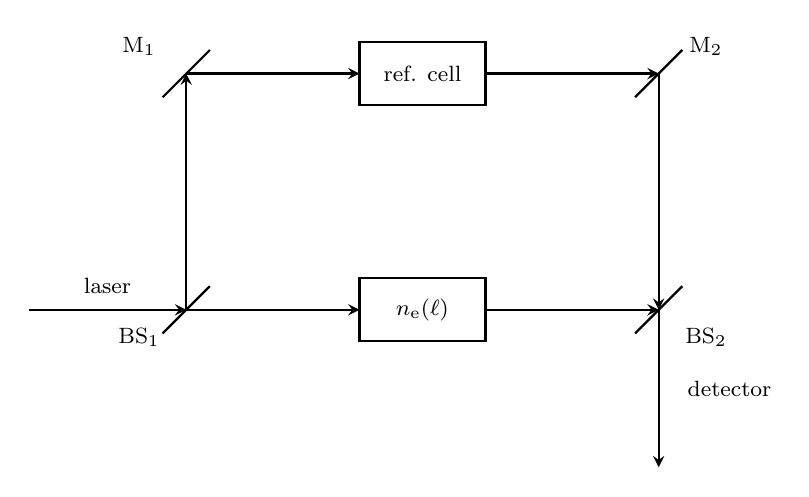
\begin{tikzpicture}[>=stealth, thick]
 \draw[->] (-2,0) -- (0,0);
 \node at (-1,0.3) {\footnotesize laser};
 \draw[->] (0,0) -- (0,3);
 \draw[->] (0,3) -- (2.2,3);
 \draw[->] (3.8,3) -- (6,3);
 \draw[->] (6,3) -- (6,0);
 \draw[->] (0,0) -- (2.2,0);
 \draw[->] (3.8,0) -- (6,0);
 \draw[->] (6,0) -- (6,-2);
 \node at (6.9,-1) {\footnotesize detector};
 \draw (2.2,-0.4) rectangle (3.8,0.4);
 \node at (3.0,0.0) {\footnotesize $n_{\mathrm{e}}(\ell)$};
 \draw (2.2,2.6) rectangle (3.8,3.4);
 \node at (3.0,3.0) {\footnotesize ref. cell};
 \draw (-0.3,-0.3) -- (0.3,0.3);
 \node at (-0.6,-0.35) {\footnotesize BS$_{1}$};
 \draw (-0.3,2.7) -- (0.3,3.3);
 \node at (-0.6,3.35) {\footnotesize M$_{1}$};
 \draw (5.7,2.7) -- (6.3,3.3);
 \node at (6.6,3.35) {\footnotesize M$_{2}$};
 \draw (5.7,-0.3) -- (6.3,0.3);
 \node at (6.6,-0.35) {\footnotesize BS$_{2}$};
\end{tikzpicture}
\caption{Schematic (illustrative, not to scale) layout of a Mach--Zehnder interferometer for line-integrated electron-density measurement. The probe beam traverses the plasma column of density $n_{\mathrm{e}}(\ell)$ along the lower arm; a reference beam of matched nominal optical path length traverses a compensating cell in the upper arm. Beamsplitters BS$_{1}$, BS$_{2}$ and mirrors M$_{1}$, M$_{2}$ recombine the two beams onto a detector, where the resulting fringe pattern encodes the phase difference of Eq.~\eqref{eq:phase-formula}.}
\label{fig:mz-schematic}
\end{figure}

\begin{figure}[htbp]
\centering
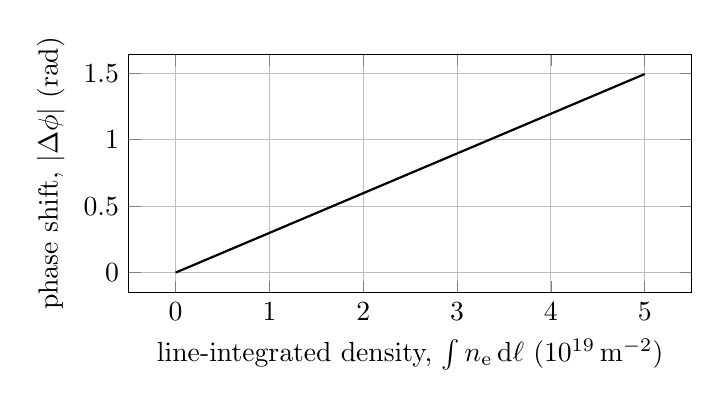
\begin{tikzpicture}
\begin{axis}[
 width=0.72\textwidth,
 height=0.38\textwidth,
 xlabel={line-integrated density, $\int n_{\mathrm{e}}\,\mathrm{d}\ell$ ($10^{19}\,\si{\per\square\meter}$)},
 ylabel={phase shift, $|\Delta\phi|$ (rad)},
 domain=0:5,
 samples=50,
 grid=major,
]
\addplot[black, thick] {0.2987*x};
\end{axis}
\end{tikzpicture}
\caption{Illustrative (analytic, not measured) phase shift at the \SI{10.6}{\micro\meter} CO$_{2}$ line, $|\Delta\phi| = r_{\mathrm{e}}\lambda \int n_{\mathrm{e}}\,\mathrm{d}\ell$ [Eq.~\eqref{eq:phase-formula}], plotted against line-integrated electron density.}
\label{fig:phase-vs-density}
\end{figure}

Because $r_{\mathrm{e}}\lambda$ is fixed once the wavelength is chosen, calibration reduces to accurate knowledge of the probe wavelength — there is no equivalent of the sheath-collection coefficient invoked by a Langmuir probe. The difficulty instead lies in engineering the phase measurement: recovering a phase to a small fraction of one fringe, continuously, despite vibration and detector noise. Homodyne systems address this in part through quadrature (I/Q) detection, combining two interferograms with a fixed $\pi/2$ phase bias to resolve magnitude and sign unambiguously, at the cost of doubled hardware.

\subsection{Heterodyne Detection}

Direct fringe-imaging Mach--Zehnder interferometry recovers $\Delta\phi$ only modulo $2\pi$ and modulo a sign, since a static fringe pattern does not indicate the direction the phase is changing. Heterodyne interferometry removes this ambiguity by imposing a small frequency offset $\Delta f$ between probe and reference beams — via an acousto-optic modulator or Zeeman-split source — so the beams beat continuously at the detector even absent plasma; the plasma-induced shift $\Delta\phi(t)$ modulates this beat signal, demodulated electronically to yield $\Delta\phi(t)$ continuously and unambiguously in sign \cite{ref0400}. It also offers large dynamic range and immunity to slow intensity drifts, since density information is carried by beat phase rather than DC intensity — the architecture of choice for CO$_{2}$-laser and millimetre-wave systems running continuously over a discharge.

\section{Multi-Chord and Dispersion Interferometry: Line-Integrated Density and Inversion}
\label{sec:interf-multichord}

\subsection{Abel Inversion for Cylindrically Symmetric Profiles}

A single chord returns only $\int n_{\mathrm{e}}\,\mathrm{d}\ell$; recovering $n_{\mathrm{e}}(r)$ requires an assumed symmetry or additional chords. For a cylindrically symmetric column and chord of impact parameter $y$, the observable is the Abel transform,
\begin{equation}
S(y) \equiv \int n_{\mathrm{e}}\,\mathrm{d}\ell = 2\int_{y}^{a} \frac{n_{\mathrm{e}}(r)\,r}{\sqrt{r^{2}-y^{2}}}\,\mathrm{d}r,
\label{eq:abel-forward}
\end{equation}
where $a$ is the plasma column radius, inverted analytically by
\begin{equation}
n_{\mathrm{e}}(r) = -\frac{1}{\pi}\int_{r}^{a} \frac{1}{\sqrt{y^{2}-r^{2}}}\,\frac{\mathrm{d}S}{\mathrm{d}y}\,\mathrm{d}y,
\label{eq:abel-inverse}
\end{equation}
which requires the derivative of the chord data with respect to impact parameter — numerically delicate in the presence of noise, so it is normally applied to a smooth fit of $S(y)$ rather than raw data. Abel inversion is exact only for genuinely axisymmetric distributions; departures from symmetry require the multi-chord tomographic approach described next.

\subsection{Multi-Chord Arrays and Tomographic Reconstruction}

Deploying an array of $N$ parallel or fan-shaped chords at distinct impact parameters $y_{i}$ converts Eq.~\eqref{eq:abel-forward} into an overdetermined linear system, $S_{i} = \sum_{j} W_{ij}\, n_{\mathrm{e},j}$, where $W_{ij}$ is a geometric weight matrix encoding the length of chord $i$ within grid cell $j$. This is solved by least-squares, singular-value decomposition, or regularised (Tikhonov) inversion to recover a tomographic density map without invoking symmetry, resolving structure Abel inversion alone cannot. In tokamaks, multi-chord interferometry provides the real-time, line-averaged density signal for feedback control of gas fuelling, its response time being fast compared with actuator timescales \cite{ref0399}.

\subsection{Two-Colour Dispersion Interferometry}

Equation~\eqref{eq:phase-formula} shows $|\Delta\phi| \propto \lambda$: the plasma phase scales as $1/\omega$. A parasitic shift from mechanical vibration instead scales as $\Delta\phi_{\mathrm{vib}} = \omega\,\delta L/c$ for a path-length change $\delta L$ — the opposite dependence. Dispersion interferometry exploits this by probing simultaneously at a fundamental frequency $\omega$ and its second harmonic $2\omega$, generated via a nonlinear crystal, so both colours traverse an identical mechanical path with the same $\delta L$ at every instant:
\begin{align}
\phi(\omega) &= \phi_{\mathrm{pl}}(\omega) + \phi_{\mathrm{vib}}(\omega)
= -\, r_{\mathrm{e}}\lambda \int n_{\mathrm{e}}\,\mathrm{d}\ell \;+\; \frac{\omega\,\delta L}{c}, \\
\phi(2\omega) &= \phi_{\mathrm{pl}}(2\omega) + \phi_{\mathrm{vib}}(2\omega)
= -\, \tfrac{1}{2} r_{\mathrm{e}}\lambda \int n_{\mathrm{e}}\,\mathrm{d}\ell \;+\; \frac{2\omega\,\delta L}{c},
\end{align}
using $\phi_{\mathrm{pl}}(2\omega) = \tfrac{1}{2}\phi_{\mathrm{pl}}(\omega)$ and $\phi_{\mathrm{vib}}(2\omega) = 2\phi_{\mathrm{vib}}(\omega)$. Forming the combination
\begin{equation}
\phi(2\omega) - 2\phi(\omega) = \tfrac{3}{2}\, r_{\mathrm{e}}\lambda \int n_{\mathrm{e}}\,\mathrm{d}\ell,
\label{eq:dispersion-interf}
\end{equation}
the vibration term cancels \emph{exactly}, to all orders in $\delta L$, leaving a signal depending on line-integrated density alone. First developed for large fusion and pulsed-power facilities, this is now standard wherever the mechanical stability of single-colour measurement (Section~\ref{sec:interf-vibration}) cannot be guaranteed \cite{ref0417}.

\section{Vibration Immunity, Wavelength Choice, and Error Sources}
\label{sec:interf-vibration}

\subsection{Sources of Phase Noise and Vibration Compensation}

Because the plasma-induced phase shift is often a small fraction of a fringe, mechanical vibration of mirrors, beamsplitters, windows, and mounts is frequently the dominant noise source, particularly for long-path systems on large devices. A path-length fluctuation $\delta L$ as small as a fraction of the probe wavelength produces a spurious excursion $\Delta\phi_{\mathrm{vib}} = 2\pi\,\delta L/\lambda$ indistinguishable, in single-colour homodyne measurement, from a genuine density change. Differential designs, sharing as much common optical path as possible, suppress uncorrelated vibration noise since a disturbance common to both arms cancels in the phase difference. Where full common-path operation is impractical, retroreflected geometries, active isolation, and, most robustly, the dispersion-cancellation scheme of Eq.~\eqref{eq:dispersion-interf} are used, insensitive to vibration by construction and preferred for pulsed-power interferometry in noisy environments \cite{ref0417}. Heterodyne detection (Section~\ref{sec:interf-phase}) adds a complementary benefit: phase from a continuously running beat signal lets low-frequency vibration appear as slow drift, distinguishable from density fluctuations of interest.

\subsection{Wavelength Trade-offs}

Table~\ref{tab:wavelengths} makes explicit the central trade-off in probe-wavelength selection. Phase sensitivity $r_{\mathrm{e}}\lambda$ increases linearly with wavelength, so long-wavelength sources (CO$_{2}$, FIR, millimetre-wave) are essential whenever line-integrated density is low, as in low-temperature, weakly ionized plasmas. Conversely, critical density falls as $\lambda^{-2}$, so those same wavelengths also suffer beam cutoff first, and are more strongly refracted by transverse gradients, since the bending angle scales with the same $\omega_{\mathrm{pe}}^{2}/\omega^{2}$ factor entering Eq.~\eqref{eq:nr-approx}. Visible and near-infrared sources remain nearly undeflected and immune to cutoff at high density, and are preferred for dense, transient plasmas requiring imaging interferometry \cite{ref0391}.

\subsection{Systematic and Statistical Error Budget}

Table~\ref{tab:errors} summarises further error sources, beyond mechanical vibration, that bound the accuracy of an interferometrically inferred density.

\begin{table}[htbp]
\centering
\caption{Principal error sources in plasma interferometry and their typical mitigation strategies. Entries are qualitative summaries of well-established diagnostic practice, not measured values from a specific experiment.}
\label{tab:errors}
\begin{tabularx}{\textwidth}{@{}l X X@{}}
\toprule
Error source & Typical origin & Mitigation \\
\midrule
Mechanical vibration & Path-length fluctuation of mirrors, windows, optical mounts & Common-path/differential design; two-colour dispersion cancellation; heterodyne detection \\
Fringe-jump ($2\pi$) ambiguity & Rapid density transients exceeding the phase-tracking bandwidth & Heterodyne phase demodulation; sufficient sampling rate; redundant chord comparison \\
Beam refraction & Transverse gradients of $n_{\mathrm{r}}$ steering the beam off the detector aperture & Wide collection optics; retroreflection; correction using measured or modelled gradients \\
Non-plasma dispersion & Vacuum windows, air path, neutral-gas background contributing to phase & Vacuum-referenced calibration shot; evacuated or purged beam path \\
Faraday-rotation crosstalk & Magnetized plasma birefringence coupling into polarization-sensitive optics & Combined polarimetry--interferometry analysis; polarization-insensitive detection \\
Finite detector/electronics bandwidth & Beat-frequency demodulation limited by photodetector or digitizer response & Bandwidth matched to expected $\dot{n}_{\mathrm{e}}$; oversampling \\
Etalon fringes & Parasitic reflections between parallel optical surfaces & Anti-reflection coatings; wedged windows; beam dumps \\
\bottomrule
\end{tabularx}
\end{table}

Fringe-jump ambiguity arises when density changes by more than one fringe within a sampling interval, so the demodulated phase folds back on itself and $\int n_{\mathrm{e}}\,\mathrm{d}\ell$ acquires an integer-fringe offset — a hazard during fast transients, mitigated by adequate sampling bandwidth and cross-checking against adjacent chords. Beam refraction, quantified by the transverse gradient of Eq.~\eqref{eq:nr-approx}, displaces the beam on the detector, potentially causing signal dropout, and imposes a small path-integration error since the ray is no longer exactly the straight chord assumed in Eq.~\eqref{eq:phase-formula}. In magnetized plasmas, birefringence responsible for Faraday rotation couples into any polarization-sensitive element and must be suppressed or exploited deliberately in combined polarimetry--interferometry systems. The non-plasma contribution to the optical path — vacuum windows, residual air, stray gas dispersion — must be removed by a reference phase measurement, since it is otherwise indistinguishable from a genuine plasma shift.

Two subtler contributions complete the budget: low-pass filtering, which attenuates genuine high-frequency structure and so must be validated against the fastest transient of interest; and the statistical noise floor of the recombined beam, which enters the phase measurement additively while the plasma shift enters linearly in density, so the minimum detectable density for a given chord length is the phase resolution divided by $r_{\mathrm{e}}\lambda L$.

\section{Role as a Fast, Robust Density Constraint}
\label{sec:interf-role}

\subsection{Non-Perturbing, Model-Independent Density Measurement}

The defining strength of interferometry, relative to every other diagnostic surveyed in this monograph, is that Eq.~\eqref{eq:phase-formula} is exact for $\omega \gg \omega_{\mathrm{pe}}$ and depends on no property of the electron population beyond its number density: not $T_{\mathrm{e}}$, not the energy-distribution shape, not any collisional--radiative assumption. By contrast, a Langmuir-probe inference requires an assumed sheath-collection model and an immersed electrode that perturbs the plasma sampled, an optical-emission inference requires a full atomic model sensitive to non-Maxwellian departures, and laser-induced fluorescence targets the ion rather than the bulk electron density. Interferometry couples to the plasma only through its linear dielectric response, leaving it undisturbed, with a formula containing no adjustable parameters beyond the known probe wavelength \cite{ref0391} — non-invasiveness and model independence that make it an external constraint against which model-dependent diagnostics, and fluid or kinetic sheath models, can be validated.

\subsection{Coupling to Sheath-Edge Flux Diagnostics}

The ion energy flux delivered to a bounding surface is controlled, in every model developed elsewhere in this monograph, by the density at the sheath edge and the ion speed there, most compactly through the Bohm velocity $u_{\mathrm{B}} = \sqrt{k_{\mathrm{B}} T_{\mathrm{e}}/m_{\mathrm{i}}}$ and a flux $\Gamma_{E} \simeq n_{\mathrm{e}} u_{\mathrm{B}} \overline{E}_{\mathrm{i}}$, where $\overline{E}_{\mathrm{i}}$ is the mean ion impact energy set by the sheath potential drop and the ion velocity distribution $f_{\mathrm{i}}(v)$ at the wall. Every quantity except $n_{\mathrm{e}}$ is set by the local electron temperature and sheath potential profile, so the absolute flux scale is fixed by the density normalization — yet a local probe or spectroscopic measurement near the sheath edge is difficult without perturbing it, and is a point measurement subject to the model dependences noted above. A line-integrated measurement along a chord intersecting the presheath and bulk plasma provides an independent, non-perturbing normalization that, combined with a presheath density-decay profile (Section~\ref{sec:interf-multichord}), can be extrapolated to the sheath edge to give an absolute prediction of $\Gamma_{E}$, resolving density transients too fast for a swept Langmuir-probe characteristic to follow \cite{ref0399,ref0417}.

\subsection{Cross-Validation with Probe and Spectroscopic Diagnostics}

In practice, interferometry rarely operates in isolation: its principal value lies in providing an absolute density benchmark against which Langmuir-probe and collisional--radiative inferences can be cross-checked, and any systematic offset identified. This role is well established in magnetically confined and processing plasmas, where multi-chord interferometry anchors the calibration of faster, more model-dependent point diagnostics; discrepancies with the probe- or spectroscopy-inferred density are themselves diagnostic of departures from assumptions — Maxwellian energy distribution, unperturbed sheath collection, local thermodynamic equilibrium — that alternative techniques must invoke \cite{ref0399}. Multi-wavelength dispersion systems further allow internal validation, since the two-colour combination of Eq.~\eqref{eq:dispersion-interf} and an independent homodyne channel should agree once vibration is accounted for \cite{ref0417}. For this monograph, interferometry supplies the density input without which the ion-energy-flux expressions of the surrounding chapters cannot be placed on an absolute scale.

\subsection{Illustrative Application Domains}

The generality of Eq.~\eqref{eq:phase-formula} means the same logic recurs across plasma regimes, differing chiefly in probe wavelength and vibration-mitigation strategy, while its role as an absolute constraint remains unchanged. In fusion research, multi-chord CO$_{2}$- or FIR-laser interferometry supplies the line-averaged core density for real-time control and absolute normalization of the edge density setting the ion flux to plasma-facing components \cite{ref0399}. In pulsed-power and z-pinch research, fibre-coupled dispersion interferometry provides dynamic, single-shot measurements through the compressing or expanding sheath \cite{ref0417}. In laser-produced plasmas, where densities approach the near-infrared critical density, ultrafast Mach--Zehnder interferometers freeze the evolution on a single shot \cite{ref0391}. In low-temperature processing plasmas — the regime most directly relevant here — millimetre-wave interferometry provides the bulk-plasma density feeding the presheath and sheath without the perturbation risked by an immersed probe \cite{ref0400}. Across every domain, the diagnostic contributes the same quantity, which is why it functions so effectively as a common density reference.

\section{Summary}
\label{sec:interf-summary}

The refractive index of an unmagnetized plasma departs from unity by an amount proportional to electron density, so the phase delay imposed on a transmitted probe beam is a direct, line-integrated, model-independent measure of $n_{\mathrm{e}}$ [Eq.~\eqref{eq:phase-formula}]. Mach--Zehnder interferometers realise this through two-beam interference and fringe imaging, while heterodyne detection removes the sign and fringe-counting ambiguities of static analysis. Multi-chord arrays and tomographic reconstruction convert line-integrated chord measurements into a spatially resolved profile via the Abel-transform relation of Eqs.~\eqref{eq:abel-forward}--\eqref{eq:abel-inverse}, and two-colour dispersion interferometry [Eq.~\eqref{eq:dispersion-interf}] exploits the opposite frequency scaling of the plasma phase shift and vibration noise to cancel the latter exactly. Probe-wavelength selection trades phase sensitivity against beam refraction and critical-density cutoff (Table~\ref{tab:wavelengths}), and a characterised error budget (Table~\ref{tab:errors}) must be applied before a phase measurement becomes an absolute density. Because the result is fast, non-perturbing, and free of the model assumptions required by probe and spectroscopic techniques, interferometry serves as the primary independent normalization for the electron density entering $\Gamma_{E}$, and as the benchmark against which every other diagnostic in this work is tested.

\chapter{Comparative Analysis and the Case for Sensor Fusion}
\label{ch:fusion}

The preceding chapters treated optical emission spectroscopy (OES), laser-induced fluorescence (LIF), Thomson scattering, and interferometry as individually capable instruments, each returning a partial description of the plasma state near a bounding wall. This chapter asks what is structurally impossible for any single diagnostic to measure, and why the ion energy flux, $\Gamma_{E}$, falls into that category. The argument concerns information content, not precision: each instrument is sensitive to a different moment, projection, or line integral of the electron and ion distribution functions, $f_{\mathrm{e}}(v)$ and $f_{\mathrm{i}}(v)$, and no finite set of scalar outputs from one technique spans the function space needed to reconstruct $\Gamma_{E}$ with a defensible uncertainty. The chapter compares the four diagnostics on observables, resolution, and invasiveness; examines their over-determination and complementarity; derives why $\Gamma_{E}$ resists single-instrument recovery; formalises the cross-calibration constraints a campaign must satisfy; and proposes a fusion architecture -- Bayesian integrated data analysis -- treating $\Gamma_{E}$ as a derived posterior quantity.

\section{Side-by-Side Comparison of the Core Diagnostics}
\label{sec:sidebyside}

\subsection{Optical Emission Spectroscopy}

OES infers electron-population properties from spontaneously emitted spectral-line intensities, via a collisional-radiative model relating excited-state populations to the electron energy distribution function (EEDF) and ground-state density \cite{ref0237}. Emission depends on an integral of the excitation cross section weighted by the local EEDF,
\begin{equation}
I_{ij} \;\propto\; n_{\mathrm{e}} \, n_{0} \int_{0}^{\infty} \sigma_{\mathrm{exc}}(v)\, v \, f_{\mathrm{e}}(v) \, \mathrm{d}v ,
\label{eq:oes_intensity}
\end{equation}
so OES returns an energy-weighted moment of $f_{\mathrm{e}}(v)$, and inferred $n_{\mathrm{e}}$, $T_{\mathrm{e}}$ are only as reliable as the assumed rate coefficients and EEDF shape. OES is passive and non-perturbing but normally line-integrated unless tomographic inversion is applied, reports electron-side quantities almost exclusively, and carries no information about the ion kinetics determining $\Gamma_{E}$. It remains a robust, low-cost diagnostic for time-resolved electron-temperature trends in thruster discharges \cite{ref0256}.

\subsection{Laser-Induced Fluorescence}

LIF probes a specific optical transition of a resonant species (commonly a metastable ion or atom state) with a narrow-linewidth, frequency-scanned laser, recording fluorescence versus detuning. The absorption profile is Doppler-shifted by the ion velocity along the laser direction, so the excitation spectrum directly reproduces a one-dimensional projection of $f_{\mathrm{i}}(v)$,
\begin{equation}
S(\nu) \;\propto\; \int_{-\infty}^{\infty} f_{\mathrm{i}}(v_{\parallel}) \, g\!\left(\nu - \nu_{0}\Big(1 + \frac{v_{\parallel}}{c}\Big)\right) \mathrm{d}v_{\parallel},
\label{eq:lif_lineshape}
\end{equation}
where $g$ is the intrinsic lineshape and $\nu_{0}$ the unshifted transition frequency. LIF is the only technique yielding the ion velocity distribution itself, in a localized volume, rather than a bulk moment \cite{ref0292}. That specificity is also its limitation: it needs an accessible, sufficiently populated resonant transition; its signal tracks the probed-state population fraction rather than total ion density; and directional flows near sheath edges and propulsion plumes can require multiple viewing geometries to unfold the full $f_{\mathrm{i}}(v)$ \cite{ref0328}.

\subsection{Thomson Scattering}

Thomson scattering illuminates the plasma with a high-power laser and analyses light scattered incoherently off free electrons, giving a direct, first-principles map of the electron velocity distribution along the scattering wavevector; in the collective regime it also resolves the ion-acoustic feature, carrying $T_{\mathrm{i}}$ and effective-charge information \cite{ref0355}. Because the cross section is a fundamental constant rather than a modelled rate coefficient, it is regarded as the most nearly first-principles determination of $n_{\mathrm{e}}$ and $T_{\mathrm{e}}$ \cite{ref0384}. Its cost is instrumental: a high-energy pulsed laser and an intrinsically weak signal ($\sim\SI{6.65e-29}{\meter\squared}$) confine measurements to a point or short chord per shot, at the laser repetition rate rather than the timescale of interest. It measures ion energy content only indirectly, not directed ion flux, and is silent on the angular distribution of ion impact governing sputtering.

\subsection{Interferometry}

Microwave or optical interferometry measures the phase shift accumulated by a probe beam, proportional to line-integrated electron density,
\begin{equation}
\Delta \phi \;=\; \frac{e^{2}}{2 m_{\mathrm{e}} \epsilon_{0} c\, \omega} \int n_{\mathrm{e}}(\ell) \, \mathrm{d}\ell ,
\label{ch11-eq:interferometry}
\end{equation}
where $\omega$ is the probe angular frequency and $\ell$ the chord. It offers excellent time resolution, negligible perturbation, and an essentially calibration-free phase--density relationship, making it a workhorse for real-time density monitoring \cite{ref0417}. Its limitation is dimensional: the observable is a line integral, recovering local $n_{\mathrm{e}}(\mathbf{r})$ requires an Abel inversion or multi-chord tomography, and it gives no information on $T_{\mathrm{e}}$, $T_{\mathrm{i}}$, or any moment of $f_{\mathrm{i}}(v)$.

\subsection{Comparative Summary}

Table~\ref{tab:diagnostic_comparison} collects the comparison, making the trade space motivating fusion explicit.

\begin{table}[htbp]
\centering
\caption{Qualitative comparison of the four core diagnostics with respect to the quantity each most directly constrains, its typical resolution character, and its degree of intrusiveness. ``Direct'' denotes an observable related to the physical quantity by a first-principles or near-first-principles relation; ``indirect'' denotes reliance on an atomic, collisional-radiative, or inversion model.}
\label{tab:diagnostic_comparison}
\begin{tabularx}{\textwidth}{@{}l X X X X@{}}
\toprule
Diagnostic & Primary observable & Access to $f_{\mathrm{i}}(v)$ & Spatial character & Perturbation \\
\midrule
OES & $n_{\mathrm{e}}$, $T_{\mathrm{e}}$ (indirect, via CR model) & None (electron-side only) & Line-integrated unless tomographic & Passive, non-perturbing \\
LIF & $f_{\mathrm{i}}(v)$ along probe axis (direct) & Direct, one velocity component per view & Localized (beam--collection overlap) & Weakly perturbing (low-intensity resonant absorption) \\
Thomson scattering & $n_{\mathrm{e}}$, $T_{\mathrm{e}}$ (direct); $T_{\mathrm{i}}$, $Z$ (collective regime, indirect fit) & Indirect, via ion-acoustic feature only & Localized (point or short chord) & Non-perturbing, but signal-limited \\
Interferometry & Line-integrated $n_{\mathrm{e}}$ (direct) & None & Chordal / tomographic & Non-perturbing \\
\bottomrule
\end{tabularx}
\end{table}

Only LIF touches the ion velocity distribution directly, and even it returns a one-dimensional projection rather than the full three-dimensional $f_{\mathrm{i}}(v)$ a general energy-flux calculation needs. No individual instrument suffices alone; recommended-practice guidance for propulsion-relevant discharges confirms that standard practice is deployment of complementary suites \cite{ref0490,ref0511}.

\subsection{Perturbation Mechanisms and Temporal Reach}

The ``perturbation'' column deserves closer reading than a simple invasive/non-invasive dichotomy, since each technique perturbs the plasma, if at all, through a distinct channel. OES and interferometry are genuinely passive; their principal risk is contamination of the measurement (stray light, window deposition, phase drift) rather than perturbation of the plasma itself. Thomson scattering cannot measurably heat the plasma at typical fluences, but the laser can produce local photoionisation or stray-light photoemission that must be characterised and subtracted \cite{ref0384}. LIF is intermediate: resonant absorption removes population from, and can saturate, the probed transition, distorting the lineshape via optical pumping unless laser intensity stays linear.

Temporal reach compounds these differences: sheaths driven by radio-frequency bias or pulsed excitation can evolve faster than several techniques' acquisition windows, since a wavelength-scanned LIF measurement averages over many sheath oscillations unless phase-locked, and a Thomson-scattering snapshot repeats only at the laser's shot rate, leaving gaps in the cycle. Interferometry, by contrast, tracks $n_{\mathrm{e}}$ continuously at bandwidths far exceeding sheath oscillation frequencies. A fused measurement of a time-varying $\Gamma_{E}(\mathbf{r},t)$ must therefore reconcile different spatial sampling volumes \emph{and} temporal apertures, developed further in Section~\ref{sec:why_no_single}.

\section{Complementarity and Over-Determination of the Plasma State}
\label{sec:complementarity}

The plasma state relevant to sheath-crossing ion energy transport can be summarised, at a point and time, by $f_{\mathrm{e}}(v)$ and $f_{\mathrm{i}}(v)$ together with the local electrostatic potential $\phi(\mathbf{r})$, coupled through Poisson's equation and quasineutrality. No diagnostic measures this full object; each measures a functional of it. The four techniques split into those constraining \emph{scalar moments} (OES and Thomson scattering for $n_{\mathrm{e}}, T_{\mathrm{e}}$, the latter also weakly for $T_{\mathrm{i}}$; interferometry for line-integrated $n_{\mathrm{e}}$), and the one constraining a \emph{functional projection} (LIF for $f_{\mathrm{i}}(v_{\parallel})$).

This split yields two benefits when deployed together. The first is \emph{over-determination}: OES, Thomson scattering, and interferometry each independently constrain $n_{\mathrm{e}}$ (OES and Thomson scattering also $T_{\mathrm{e}}$), so a campaign has more constraints than the minimum needed -- the raw material of cross-calibration (Section~\ref{sec:crosscal}) and outlier rejection, since agreement within stated uncertainty raises confidence in both instruments while disagreement is itself diagnostic of a systematic error or model deficiency.

The second benefit is \emph{complementarity}: LIF supplies information -- the shape of $f_{\mathrm{i}}(v)$, including any non-Maxwellian tail from sheath acceleration, charge-exchange collisions, or presheath ionisation -- absent from the other three techniques' output space. Even a perfect measurement of $n_{\mathrm{e}}$ and $T_{\mathrm{e}}$ leaves the ion distribution unconstrained beyond whatever closure the analyst imposes, and this cannot be manufactured by adding more instruments of the same class. Over-determination multiplies confidence in already-accessible quantities; complementarity extends the accessible quantity set altogether.

A diagnostic suite should therefore maximise both properties: enough electron-side overlap for rigorous cross-calibration, and at least one technique -- here, LIF -- reaching ion kinetic degrees of freedom the electron-side techniques cannot see. Bayesian integrated data analysis frameworks developed for magnetic-confinement devices formalise this logic, combining heterogeneous diagnostics with different forward models into a single joint inference of the plasma state \cite{ref0707,ref0712,ref0706}.

Framed in information-content terms, each diagnostic supplies a small number of ``channels'' -- functionals through which information about the unknown plasma state $\boldsymbol\theta$ can pass. A second interferometer chord or OES viewing line adds channels devoted to moments already accessible to those techniques, tightening the posterior there but leaving the ion-distribution directions unconstrained; adding LIF, or a second LIF viewing angle, opens genuinely new channels into the velocity-space structure of $f_{\mathrm{i}}(v)$ that no amount of additional density channels can reach. Over-determination reduces \emph{variance} in already-observable directions; complementarity extends the \emph{rank} of the observation operator. A fusion architecture that only accumulates over-determining instruments therefore yields an increasingly precise but structurally incomplete $\Gamma_{E}$, since $q_{\mathrm{i}}$ remains in the unobserved null space until a distribution-resolving diagnostic such as LIF is included.

\section{Why No Single Diagnostic Recovers the Ion Energy Flux}
\label{sec:why_no_single}

\subsection{The ion energy flux as a kinetic moment}

The ion energy flux crossing a wall-normal surface is the second-order (energy-weighted) moment of $f_{\mathrm{i}}(v)$ along the surface normal,
\begin{equation}
\Gamma_{E}(\mathbf{r}, t) \;=\; \int_{0}^{\infty} \frac{1}{2} m_{\mathrm{i}} v^{2} \; v \, f_{\mathrm{i}}(v; \mathbf{r}, t) \, \mathrm{d}v ,
\label{eq:gammaE_def}
\end{equation}
with units $\si{\watt\per\meter\squared}$ once $f_{\mathrm{i}}(v)$ is normalised so $\int f_{\mathrm{i}}(v)\,\mathrm{d}v = n_{\mathrm{i}}$. Writing $v = u_{\mathrm{i}} + w$, with $u_{\mathrm{i}} = \langle v \rangle$ the mean ion velocity and $w$ the peculiar velocity, decomposes this into bulk and kinetic contributions:
\begin{align}
\Gamma_{E} &= n_{\mathrm{i}} u_{\mathrm{i}} \left( \frac{1}{2} m_{\mathrm{i}} u_{\mathrm{i}}^{2} + \frac{5}{2} T_{\mathrm{i}} \right) + q_{\mathrm{i}}, \label{eq:gammaE_decomp} \\
q_{\mathrm{i}} &= \int_{-\infty}^{\infty} \frac{1}{2} m_{\mathrm{i}} w^{2} \, w \, f_{\mathrm{i}}(w) \, \mathrm{d}w. \label{eq:heatflux_def}
\end{align}
The first term is the directed kinetic-plus-thermal energy flux carried by the bulk drift, expressible entirely through $n_{\mathrm{i}}$, $u_{\mathrm{i}}$, $T_{\mathrm{i}}$. The second, $q_{\mathrm{i}}$, is the conductive heat flux -- the third central moment of $f_{\mathrm{i}}(v)$ -- vanishing only if $f_{\mathrm{i}}(v)$ is exactly a (possibly drifting) Maxwellian. Sheath-accelerated ion populations generally are not: kinetic theory and particle simulations of the presheath--sheath transition consistently show skewed, cut off, or bimodal distributions, so $q_{\mathrm{i}} \neq 0$ is expected rather than exceptional near a wall.

\subsection{The moment-access argument}

Table~\ref{tab:diagnostic_comparison} can now be read as a statement about which terms of Equation~\eqref{eq:gammaE_decomp} each diagnostic constrains.

\begin{itemize}
\item \textbf{OES} constrains $n_{\mathrm{e}}$, $T_{\mathrm{e}}$ via Equation~\eqref{eq:oes_intensity}; neither appears explicitly in Equation~\eqref{eq:gammaE_decomp}. $T_{\mathrm{e}}$ enters $\Gamma_{E}$ only indirectly, via the presheath potential drop and the Bohm speed $u_{\mathrm{B}} = \sqrt{T_{\mathrm{e}}/m_{\mathrm{i}}}$; OES alone cannot fix $u_{\mathrm{i}}$, $T_{\mathrm{i}}$, or $q_{\mathrm{i}}$.
\item \textbf{Thomson scattering} constrains $n_{\mathrm{e}}$, $T_{\mathrm{e}}$ directly and, in the collective regime, a weighted $T_{\mathrm{i}}$, but supplies no $u_{\mathrm{i}}$ or $q_{\mathrm{i}}$, and its $T_{\mathrm{i}}$ presupposes a Maxwellian closure in the spectral fit \cite{ref0355}.
\item \textbf{Interferometry} constrains only line-integrated $n_{\mathrm{e}}$ (Equation~\eqref{ch11-eq:interferometry}), entering $\Gamma_{E}$ solely through density normalisation, with no energy information.
\item \textbf{LIF} constrains the shape of $f_{\mathrm{i}}(v_{\parallel})$ (Equation~\eqref{eq:lif_lineshape}), in principle sufficient to compute $u_{\mathrm{i}}$, $T_{\mathrm{i}}$, and $q_{\mathrm{i}}$ from its first three moments -- \emph{provided} the absolute ion density is supplied externally, since fluorescence intensity tracks the (generally unknown, quenching-affected) probed-state population, not $n_{\mathrm{i}}$ itself.
\end{itemize}

The crux: LIF alone accesses the higher moments of $f_{\mathrm{i}}(v)$ determining $q_{\mathrm{i}}$, but cannot deliver an absolutely calibrated $\Gamma_{E}$ without an independently supplied density scale, since its raw signal carries only \emph{relative} shape information unless calibrated against a known scatterer or density -- a route rarely available in situ \cite{ref0292}. The three density/temperature diagnostics, conversely, supply that absolute scale with high confidence but are blind to $q_{\mathrm{i}}$. $\Gamma_{E}$ is therefore a genuinely joint product, requiring the density scale from OES, Thomson scattering, or interferometry, and the distribution shape from LIF, evaluated self-consistently at the same location and instant -- consistent with the broader finding that single-instrument inference of any moment beyond second order systematically underestimates true uncertainty, since the closure assumption substitutes for missing information \cite{ref0711}.

\subsection{A further obstruction: geometry and species mixing}

Two obstructions compound the moment-access problem. First, $\Gamma_{E}$ is a flux through a specific surface orientation; if ions arrive with a spread of incidence angles (oblique magnetic field, or multiple presheath ionisation sources), a single LIF chord samples only one velocity projection and misrepresents the angle-integrated flux unless multiple non-collinear views are combined \cite{ref0328}. Second, in gases with multiple charge states or species, each contributes its own term to Equation~\eqref{eq:gammaE_def}, and OES, Thomson scattering, and interferometry are essentially blind to that partition; only species- or charge-resolved probing, which LIF can in principle provide, recovers it. Every diagnostic here samples only a low-dimensional projection of a high-order functional of the plasma state.

\subsection{Time-varying sheaths and the mismatch of temporal apertures}

A further obstruction concerns time dependence. Where the sheath potential oscillates, as under radio-frequency bias or pulsed excitation, $\Gamma_{E}(\mathbf{r},t)$ is a time series, and Equation~\eqref{eq:gammaE_decomp} must in principle be evaluated at each phase of the drive cycle. The four diagnostics sample this series through the very different apertures noted in Section~\ref{sec:sidebyside}, so combining a phase-resolved density trace with a phase-averaged LIF shape, without an explicit model of how each observable maps onto the time-dependent state, would silently conflate an instantaneous quantity with a cycle-averaged one. Section~\ref{sec:architecture}'s forward-model formalism resolves this by including each instrument's acquisition-window function explicitly in $M_{k}(\boldsymbol{\theta})$, so a candidate state $\boldsymbol{\theta}(t)$ is compared against data only after convolution with its actual temporal aperture.

\section{Cross-Calibration and Consistency Constraints}
\label{sec:crosscal}

Because $\Gamma_{E}$ must be assembled from several instruments' outputs, its reliability depends on whether those outputs are mutually consistent once transformed to a common physical basis. This section formalises the consistency requirements a multi-diagnostic campaign should satisfy before its outputs feed a fused estimate.

\subsection{Overlap constraints on $n_{\mathrm{e}}$ and $T_{\mathrm{e}}$}

Because OES, Thomson scattering, and interferometry all constrain $n_{\mathrm{e}}$ (OES and Thomson scattering also $T_{\mathrm{e}}$), each pair produces an independent consistency check via a normalised residual for a pair $(a, b)$ measuring the same quantity $X \in \{n_{\mathrm{e}}, T_{\mathrm{e}}\}$ at coincident space-time points,
\begin{equation}
\chi_{ab}^{2} \;=\; \frac{\left(X_{a} - X_{b}\right)^{2}}{\sigma_{a}^{2} + \sigma_{b}^{2}},
\label{eq:chi2_pairwise}
\end{equation}
with $\sigma_{a}, \sigma_{b}$ the one-standard-deviation uncertainties. A campaign with $\chi_{ab}^{2} \sim O(1)$ across all pairs and conditions is internally consistent; systematic excursions well above unity signal an unmodelled effect, such as inaccurate excitation cross sections or a drifting calibration. Comparisons of Langmuir-probe, Thomson scattering, and optical techniques in magnetron discharges confirm such agreement is regime-dependent rather than universal \cite{ref0355}.

\subsection{Absolute calibration anchoring}

Not all instruments are equally trustworthy as absolute scales. Thomson scattering, whose cross section is a QED constant independent of atomic structure, is the closest available approximation to a first-principles standard for $n_{\mathrm{e}}$ and $T_{\mathrm{e}}$ \cite{ref0384}, and Bayesian treatments of its spectra propagate this calibration confidence into the posterior rather than treating it as fixed and error-free \cite{ref0684}. Interferometry, governed by a purely classical dispersion relation, is similarly close to calibration-free. OES and LIF depend on modelled or externally supplied normalisation constants and are properly treated as \emph{relative} techniques that borrow their absolute scale from the anchor instruments: a coherent strategy uses Thomson scattering and/or interferometry to fix the absolute density (and, for Thomson scattering, temperature) scale, then propagates it into the OES inversion and the LIF normalisation.

\subsection{Spatial and temporal registration}

A consistency check of the kind in Equation~\eqref{eq:chi2_pairwise} is only meaningful if the compared quantities refer to the same location and instant, which is nontrivial given the four techniques' different measurement volumes and integration times: OES and interferometry are frequently line-integrated, Thomson scattering is a short-pulse point or chord measurement, and LIF integrates over a finite beam-collection volume and, for a wavelength scan, a finite acquisition time. Any fused estimate of $\Gamma_{E}$ must therefore carry an explicit \emph{registration model} -- a forward mapping from the assumed local state to what each instrument would report given its sampling geometry and window -- the role played by the ``forward model'' in Bayesian integrated data analysis \cite{ref0713}. Neglecting registration is a common source of apparent inconsistency; recommended-practice guidance for propulsion and processing-plasma diagnostics emphasises standardising acquisition geometry and timing to minimise it \cite{ref0511,ref0490}.

\subsection{Consistency as a diagnostic in its own right}

Persistent, well-characterised disagreement between instruments, once registration and calibration anchoring are accounted for, is not a campaign failure but a source of physical information. A systematic offset between Thomson-scattering $T_{\mathrm{i}}$ (from the ion-acoustic feature under a Maxwellian closure) and LIF-derived $T_{\mathrm{i}}$ (from the second moment of the directly measured $f_{\mathrm{i}}(v)$) is itself evidence of non-Maxwellian structure, since the two would agree exactly were the closure assumption exact -- an additional channel of physical inference about the higher-order moments, $q_{\mathrm{i}}$ foremost, motivating the fusion architecture of Section~\ref{sec:architecture}.

\subsection{A worked illustration of pairwise inconsistency}

To make Equation~\eqref{eq:chi2_pairwise} concrete, consider a hypothetical (illustrative, not measured) exercise in which OES and interferometry both report the electron density near the sheath edge. Interferometry, the near-calibration-free anchor, returns $n_{\mathrm{e}} = \SI{5.0e17}{\per\cubic\meter}$ with $\SI{5}{\percent}$ uncertainty; OES, inverted at an assumed $T_{\mathrm{e}} = \SI{3.0}{\electronvolt}$, returns $n_{\mathrm{e}} = \SI{7.5e17}{\per\cubic\meter}$ with $\SI{15}{\percent}$ uncertainty, dominated by excitation-rate-coefficient uncertainty. Propagating both into Equation~\eqref{eq:chi2_pairwise} gives $\chi^{2}_{ab} \approx 4.7$, well above the $O(1)$ threshold expected of consistent measurements. Since interferometry carries lower relative uncertainty, the natural response is to interrogate the OES model rather than average the two values: a biased assumed $T_{\mathrm{e}}$ propagates directly into a biased inferred $n_{\mathrm{e}}$ through the excitation cross section. Adopting an anchored $T_{\mathrm{e}}$ as external input should push the residual toward unity; persistence points to a deeper deficiency. Pairwise residuals are thus used diagnostically, not merely reported \cite{ref0355}.

\section{Conceptual Architecture of the Fused Measurement}
\label{sec:architecture}

\subsection{From instrument outputs to a single plasma-state posterior}

The preceding sections establish that $\Gamma_{E}$ cannot be read off any single instrument and must be assembled from heterogeneous, differently calibrated observables. The natural framework is Bayesian integrated data analysis (IDA), in which a state vector $\boldsymbol{\theta} = \{n_{\mathrm{e}}(\mathbf{r}), T_{\mathrm{e}}(\mathbf{r}), f_{\mathrm{i}}(v; \mathbf{r})\}$ on a grid spanning the presheath and sheath is inferred jointly from all diagnostic data sets $\{d_{k}\}$ via Bayes' theorem,
\begin{equation}
p(\boldsymbol{\theta} \mid \{d_{k}\}) \;\propto\; p(\boldsymbol{\theta}) \prod_{k} p(d_{k} \mid \boldsymbol{\theta}),
\label{eq:bayes_ida}
\end{equation}
where $p(\boldsymbol{\theta})$ encodes prior physical knowledge (e.g. the Bohm criterion, or smoothness of $n_{\mathrm{e}}(\mathbf{r})$) and each likelihood $p(d_{k} \mid \boldsymbol{\theta})$ is built from a forward model $M_{k}(\boldsymbol{\theta})$ synthesising the expected reading of instrument $k$ under an instrument-specific noise model,
\begin{equation}
p(d_{k} \mid \boldsymbol{\theta}) \;\propto\; \exp\!\left[-\frac{1}{2}\left(d_{k} - M_{k}(\boldsymbol{\theta})\right)^{\!\top} \Sigma_{k}^{-1} \left(d_{k} - M_{k}(\boldsymbol{\theta})\right)\right].
\label{eq:likelihood_k}
\end{equation}
This formalism has been demonstrated for joint inference of kinetic profiles with magnetic equilibrium reconstruction \cite{ref0706}, combination of heterogeneous fusion diagnostics under a single probabilistic model \cite{ref0707}, and multi-diagnostic Bayesian modelling at stellarator and tokamak facilities \cite{ref0713}. Here the four forward models are $M_{\mathrm{OES}}(\boldsymbol{\theta})$ from Equation~\eqref{eq:oes_intensity}; $M_{\mathrm{Thomson}}(\boldsymbol{\theta})$ from the scattering spectrum; $M_{\mathrm{interf}}(\boldsymbol{\theta})$, the line integral of Equation~\eqref{ch11-eq:interferometry}; and $M_{\mathrm{LIF}}(\boldsymbol{\theta})$, the convolution of Equation~\eqref{eq:lif_lineshape} with the instrument function. Once $p(\boldsymbol{\theta} \mid \{d_{k}\})$ is obtained -- by direct maximisation for a Gaussian-linearised problem, or Markov-chain Monte Carlo otherwise \cite{ref0710,ref0727} -- $\Gamma_{E}$ is computed as a \emph{derived} quantity via Equation~\eqref{eq:gammaE_def} on posterior samples, so its uncertainty is a physically consistent propagation of all instrument uncertainties and forward-model imperfections rather than an ad hoc combination of separately reported error bars.

\subsection{Schematic data flow}

Figure~\ref{fig:fusion_architecture} sketches this architecture. Raw outputs from the four diagnostics feed forward models compared, inside the inference engine, against a candidate plasma-state trajectory constrained by sheath-physics priors (quasineutrality, the Bohm criterion, Poisson's equation in the collisionless or weakly collisional limit), yielding a posterior over $\Gamma_{E}(\mathbf{r}, t)$ from which a point estimate and uncertainty interval are extracted.

\begin{figure}[htbp]
\centering
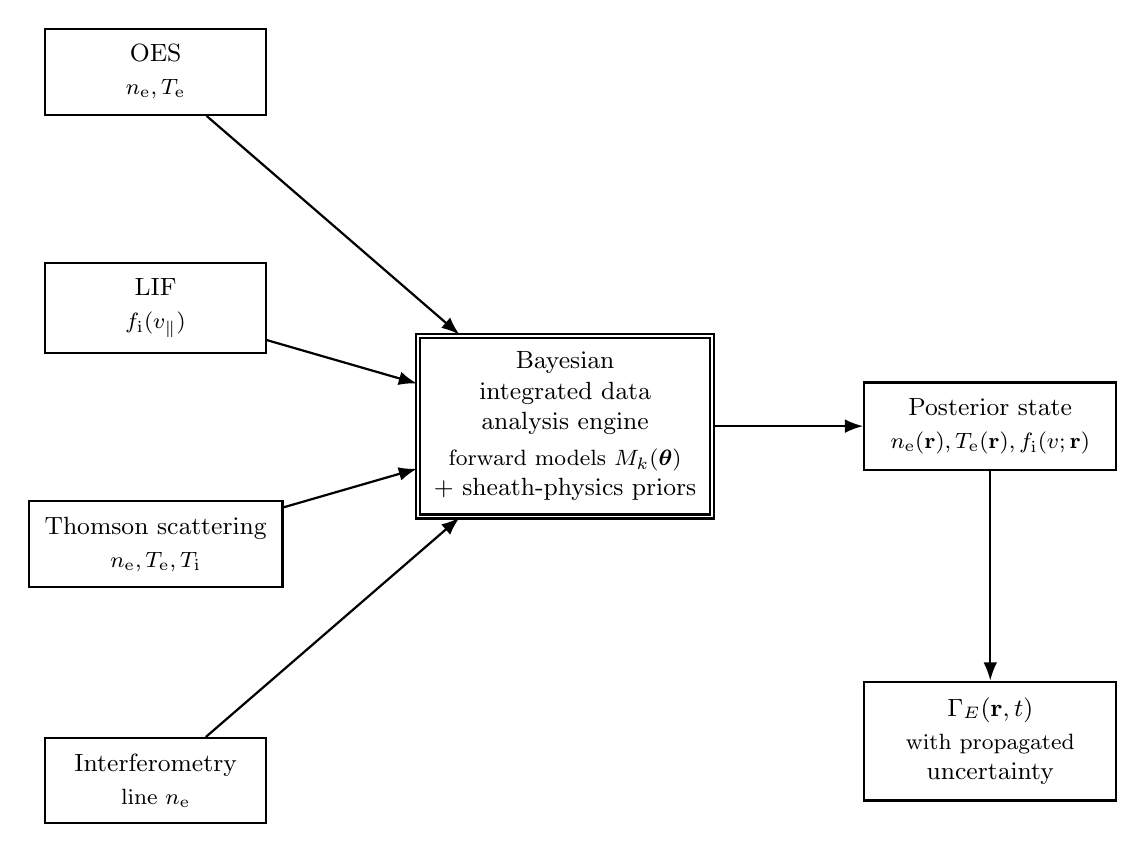
\begin{tikzpicture}[
 node distance=8mm and 14mm,
 every node/.style={font=\small},
 box/.style={draw, thick, rectangle, align=center, minimum height=9mm, minimum width=28mm, inner sep=2mm},
 engine/.style={draw, thick, rectangle, align=center, minimum height=16mm, minimum width=34mm, inner sep=2mm, double},
 arr/.style={-Latex, thick}
]
 \node[box] (oes) at (0,4.5) {OES\\[1pt]\footnotesize $n_{\mathrm{e}}, T_{\mathrm{e}}$};
 \node[box] (lif) at (0,1.5) {LIF\\[1pt]\footnotesize $f_{\mathrm{i}}(v_{\parallel})$};
 \node[box] (ts) at (0,-1.5) {Thomson scattering\\[1pt]\footnotesize $n_{\mathrm{e}}, T_{\mathrm{e}}, T_{\mathrm{i}}$};
 \node[box] (interf) at (0,-4.5) {Interferometry\\[1pt]\footnotesize line $n_{\mathrm{e}}$};

 \node[engine] (engine) at (5.2,0) {Bayesian\\integrated data\\analysis engine\\[2pt]\footnotesize forward models $M_{k}(\boldsymbol{\theta})$\\ + sheath-physics priors};

 \node[box, minimum width=32mm] (state) at (10.6,0) {Posterior state\\[1pt]\footnotesize $n_{\mathrm{e}}(\mathbf r), T_{\mathrm{e}}(\mathbf r), f_{\mathrm{i}}(v;\mathbf r)$};

 \node[box, minimum width=32mm, minimum height=12mm] (out) at (10.6,-4) {$\Gamma_{E}(\mathbf r,t)$\\[1pt]\footnotesize with propagated\\uncertainty};

 \draw[arr] (oes) -- (engine);
 \draw[arr] (lif) -- (engine);
 \draw[arr] (ts) -- (engine);
 \draw[arr] (interf) -- (engine);
 \draw[arr] (engine) -- (state);
 \draw[arr] (state) -- (out);
\end{tikzpicture}
\caption{Schematic (illustrative, not measured) conceptual architecture for a fused ion-energy-flux estimate. Four heterogeneous diagnostics supply data to instrument-specific forward models inside a Bayesian integrated data analysis engine, which combines them with sheath-physics priors to produce a posterior plasma state; the ion energy flux $\Gamma_{E}$ is then evaluated as a derived moment of that posterior, carrying a propagated, cross-instrument uncertainty rather than a single-instrument error bar.}
\label{fig:fusion_architecture}
\end{figure}

\subsection{Priors from sheath theory}

The prior $p(\boldsymbol{\theta})$ is where the sheath-theoretic content of this monograph enters the fusion architecture. Rather than leaving $n_{\mathrm{e}}(\mathbf{r})$, $T_{\mathrm{e}}(\mathbf{r})$, and $f_{\mathrm{i}}(v; \mathbf{r})$ unconstrained, it can encode the Bohm criterion as a soft constraint on ion drift speed at the sheath edge, the monotonic decay of $n_{\mathrm{e}}$ toward the wall, and a parameterised family of $f_{\mathrm{i}}(v)$ shapes (Maxwellian, shifted Maxwellian, or a truncated/skewed form) rather than an unrestricted nonparametric distribution. Such priors regularise the inversion where coverage is sparse and state explicitly which features of the inferred $\Gamma_{E}$ are data-driven versus prior-driven \cite{ref0709}.

\subsection{Surrogate models for tractability}

A full nonlinear Bayesian inversion with expensive forward models (a collisional-radiative solve for OES, a kinetic sheath solve for the LIF-constrained closure) can be prohibitively slow for time-resolved or high-throughput analysis. A practical resolution, already demonstrated for profile inference at stellarator facilities, is training fast neural-network surrogates for the forward models or the posterior itself, cutting inference time by orders of magnitude while retaining calibrated uncertainty \cite{ref0728,ref0731}. Such surrogates transfer directly to a sheath-diagnostics pipeline, allowing near-real-time evaluation of $\Gamma_{E}(\mathbf{r}, t)$ from streaming data -- essential for a live process-control or thruster-health signal rather than a post-hoc tool \cite{ref0719}.

\subsection{Tomographic extensions}

Where any instrument is deployed in a multi-chord or multi-view configuration, the architecture extends naturally to a joint tomographic inversion, with $M_{k}(\boldsymbol{\theta})$ mapping a two- or three-dimensional state onto the full set of observations and Gaussian-process priors enforcing spatial smoothness, as demonstrated for combined Thomson scattering and interferometer diagnostics \cite{ref0683}; model-selection methods in comparable settings prevent overfitting in underdetermined, multi-instrument divertor geometries \cite{ref0685}. Extending the architecture this way would resolve $\Gamma_{E}(\mathbf{r}, t)$ across the footprint of an extended plasma-facing surface -- the natural end goal for spatially resolved erosion or heat-load prediction.

\subsection{Validation loop}

A fused measurement architecture is only as trustworthy as its validation: the same posterior machinery that produces $\Gamma_{E}$ also produces posterior-predictive checks, where synthetic readings generated from posterior samples of $\boldsymbol{\theta}$ are compared against held-out or independently acquired data, closing the loop with the cross-calibration constraints of Section~\ref{sec:crosscal}. Systematic reviews of integrated data analysis identify this validation step, not the inference step itself, as the primary determinant of whether a fused quantity can be trusted for design decisions \cite{ref0712}.

\section{Summary}
\label{sec:fusion_summary}

This chapter has argued, on structural rather than practical grounds, that $\Gamma_{E}$ cannot be recovered from any single diagnostic among OES, LIF, Thomson scattering, and interferometry. Each accesses a different, low-order projection or moment of the electron and ion distribution functions: OES and Thomson scattering constrain electron-side density and temperature; interferometry constrains line-integrated density with essentially no calibration overhead; and LIF alone reaches the ion velocity distribution, but only as a relative, one-dimensional projection requiring external density anchoring. Because $\Gamma_{E}$ decomposes into a bulk convective term set by density, drift, and temperature, and a conductive heat-flux term set by the third moment of $f_{\mathrm{i}}(v)$, no diagnostic subset omitting either the density scale or the ion-distribution shape delivers a complete estimate. The four techniques are simultaneously over-determined -- enabling rigorous cross-calibration -- and complementary, since only LIF supplies the higher-moment ion information the others cannot provide at any amount of deployment. A coherent campaign must enforce explicit consistency constraints -- pairwise residual checks, calibration anchoring, and spatial/temporal registration -- before combining outputs via Bayesian integrated data analysis, which fuses instrument-specific forward models and sheath-physics priors into a single posterior plasma state from which $\Gamma_{E}$ is evaluated with propagated, physically grounded uncertainty. This architecture, with its surrogate-model and tomographic extensions, sets the stage for the quantitative fusion methodology that follows.

\chapter{Fluid Modelling of Plasmas and Sheaths}
\label{ch:fluid}

Earlier chapters track the full distribution functions $f_{\mathrm{e}}(\mathbf{r},\mathbf{v},t)$ and $f_{\mathrm{i}}(\mathbf{r},\mathbf{v},t)$ under the Boltzmann equation, resolving non-Maxwellian tails, trapped populations and the fine structure of the ion energy distribution at a wall. That completeness is expensive: a kinetic solve of the plasma-sheath system is a high-dimensional phase-space problem repeated for every density, temperature and bias explored, and inverting a measured ion energy flux $\Gamma_{E}$ onto bulk plasma parameters may need thousands of forward evaluations, more than a kinetic solver can sustain inside an optimisation loop or Markov-chain sampler. Fluid models close this gap: velocity moments of the Boltzmann equation yield a hierarchy of macroscopic conservation laws for density, momentum and energy that, once truncated by a closure hypothesis, reduce to a small system of differential equations in space and time alone. This chapter develops that hierarchy, catalogues common closures, derives the classical fluid sheath model and the Bohm criterion it implies, discusses where the fluid approximation fails near the sheath edge, specifies the boundary conditions coupling a fluid presheath to the sheath, and connects the formalism to the forward-modelling needs of the ion energy flux inversion at the centre of this monograph.

\section{Moments of the Boltzmann Equation}
\label{sec:moments}

\subsection{The kinetic starting point}

For each species $s\in\{\mathrm{e},\mathrm{i}\}$, with mass $m_s$, charge $q_s$ and distribution function $f_s(\mathbf{r},\mathbf{v},t)$ normalised so that $n_s(\mathbf{r},t)=\int f_s\,\mathrm{d}^3v$, the Boltzmann equation reads
\begin{equation}
\frac{\partial f_s}{\partial t} + \mathbf{v}\cdot\nabla f_s + \frac{q_s}{m_s}\left(\mathbf{E}+\mathbf{v}\times\mathbf{B}\right)\cdot\nabla_{\mathbf{v}} f_s = C_s[f_s],
\label{ch12-eq:boltzmann}
\end{equation}
where $C_s[f_s]$ is the collision operator, covering elastic Coulomb collisions, charge exchange, ionisation and recombination. The fluid approach integrates this against successive powers of $\mathbf{v}$, the procedure underlying the first-principles derivation of the Bohm criterion \cite{ref0670}; every fluid sheath model below is a truncation of this hierarchy.

Define the moments
\begin{align}
n_s(\mathbf{r},t) &= \int f_s\,\mathrm{d}^3v, \label{eq:mom0}\\
n_s\mathbf{u}_s(\mathbf{r},t) &= \int \mathbf{v}\,f_s\,\mathrm{d}^3v, \label{eq:mom1}\\
\mathsf{P}_s(\mathbf{r},t) &= m_s\int (\mathbf{v}-\mathbf{u}_s)(\mathbf{v}-\mathbf{u}_s)\,f_s\,\mathrm{d}^3v, \label{eq:mom2}\\
\mathbf{q}_s(\mathbf{r},t) &= \frac{m_s}{2}\int (\mathbf{v}-\mathbf{u}_s)\,|\mathbf{v}-\mathbf{u}_s|^2\,f_s\,\mathrm{d}^3v, \label{eq:mom3}
\end{align}
the density, mean fluid velocity, pressure tensor and heat flux vector. The scalar pressure is $p_s = \tfrac{1}{3}\operatorname{Tr}\mathsf{P}_s$, and for a Maxwellian $\mathsf{P}_s = p_s\mathsf{I}$ with $p_s = n_s T_s$ (temperature in energy units throughout). These four moments underlie every two-fluid and drift-diffusion model below.

\subsection{The moment hierarchy}

Multiplying Eq.~\eqref{ch12-eq:boltzmann} by $1$, $m_s\mathbf{v}$ and $\tfrac{1}{2}m_s v^2$ and integrating over velocity space produces three exact conservation equations, with source and exchange terms redistributed between species by collisions.

\subsubsection{Zeroth moment: continuity}

Integrating Eq.~\eqref{ch12-eq:boltzmann} over velocity space, with the electromagnetic term vanishing on integration by parts, gives continuity,
\begin{equation}
\frac{\partial n_s}{\partial t} + \nabla\cdot(n_s\mathbf{u}_s) = S_s,
\label{eq:continuity}
\end{equation}
where $S_s = \int C_s[f_s]\,\mathrm{d}^3v$ is the net particle source, dominated in low-temperature discharges by electron-impact ionisation, $S_s = n_{\mathrm{e}} n_{\mathrm{n}} k_{\mathrm{iz}}(T_{\mathrm{e}})$. In the collisionless sheath $S_s\to0$, and Eq.~\eqref{eq:continuity} reduces in steady, one-dimensional, planar geometry to flux conservation,
\begin{equation}
n_s(x)\,u_s(x) = \Gamma_s = \mathrm{const},
\label{eq:flux-conservation}
\end{equation}
the single most useful fluid relation for sheath analysis, underlying nearly every closed-form solution in Sec.~\ref{sec:sheath-models} \cite{ref0013}.

\subsubsection{First moment: momentum}

Multiplying Eq.~\eqref{ch12-eq:boltzmann} by $m_s\mathbf{v}$ and integrating yields
\begin{equation}
m_s n_s\left(\frac{\partial \mathbf{u}_s}{\partial t} + \mathbf{u}_s\cdot\nabla\mathbf{u}_s\right) = q_s n_s\left(\mathbf{E}+\mathbf{u}_s\times\mathbf{B}\right) - \nabla\cdot\mathsf{P}_s + \mathbf{R}_s,
\label{eq:momentum}
\end{equation}
where $\mathbf{R}_s$ is the mean momentum-transfer rate from collisions with other species. For a scalar pressure closure, $\nabla\cdot\mathsf{P}_s = \nabla p_s$, and in unmagnetised, one-dimensional, steady, collisionless conditions this reduces to the ion equation of motion of classical sheath theory,
\begin{equation}
m_{\mathrm{i}} n_{\mathrm{i}} u_{\mathrm{i}}\frac{\mathrm{d}u_{\mathrm{i}}}{\mathrm{d}x} = -q_{\mathrm{i}} n_{\mathrm{i}}\frac{\mathrm{d}\phi}{\mathrm{d}x} - \frac{\mathrm{d}p_{\mathrm{i}}}{\mathrm{d}x}.
\label{eq:ion-momentum-1d}
\end{equation}
Combined with Poisson's equation this yields the Bohm criterion (Sec.~\ref{sec:sheath-models}). For electrons, whose thermal speed vastly exceeds the ion fluid velocity, inertia is negligible on sheath scales and Eq.~\eqref{eq:momentum} truncates to a balance between electric force and pressure gradient, $0 = e n_{\mathrm{e}} \mathrm{d}\phi/\mathrm{d}x - \mathrm{d}p_{\mathrm{e}}/\mathrm{d}x$, which for an isothermal electron fluid integrates to the Boltzmann relation
\begin{equation}
n_{\mathrm{e}}(x) = n_{\mathrm{e}0}\exp\!\left(\frac{e\phi(x)}{T_{\mathrm{e}}}\right),
\label{eq:boltzmann-electrons}
\end{equation}
with $\phi\le0$ relative to the bulk plasma. This, with the ion momentum equation, defines the two closures of the standard fluid sheath model.

\subsubsection{Second moment: energy}

Multiplying Eq.~\eqref{ch12-eq:boltzmann} by $\tfrac{1}{2}m_s v^2$ and integrating, and writing total energy density as $\tfrac{3}{2}n_sT_s + \tfrac{1}{2}m_sn_su_s^2$, the internal-energy part obeys
\begin{equation}
\frac{3}{2}\left(\frac{\partial p_s}{\partial t} + \mathbf{u}_s\cdot\nabla p_s\right) + \frac{5}{2}p_s\nabla\cdot\mathbf{u}_s = -\nabla\cdot\mathbf{q}_s - \mathsf{P}_s:\nabla\mathbf{u}_s + Q_s,
\label{eq:energy}
\end{equation}
where $Q_s$ collects collisional heating and cooling; the viscous-stress term is usually negligible for weakly collisional low-temperature plasmas. This equation would fix $T_{\mathrm{e}}(x)$ and $T_{\mathrm{i}}(x)$ self-consistently, but introduces the heat flux $\mathbf{q}_s$, itself governed by a fourth-order moment, and so on indefinitely: the closure problem of Sec.~\ref{sec:closure}.

\subsection{The ion energy flux as a fluid moment}

The quantity of central interest here, the ion energy flux at a bounding surface $\Gamma_{E}$, is itself a moment of $f_{\mathrm{i}}(v)$,
\begin{equation}
\Gamma_{E} = \int_0^{\infty} \tfrac{1}{2}m_{\mathrm{i}} v^2 \, f_{\mathrm{i}}(v)\, v\,\mathrm{d}v,
\label{eq:GammaE-kinetic}
\end{equation}
evaluated at the wall, with $f_{\mathrm{i}}(v)$ the wall-directed ion velocity distribution. In fluid language this is
\begin{equation}
\Gamma_{E} = n_{\mathrm{i}} u_{\mathrm{i}}\left(\tfrac{1}{2}m_{\mathrm{i}}u_{\mathrm{i}}^2 + \tfrac{5}{2}T_{\mathrm{i}}\right) + q_{\mathrm{i}},
\label{eq:GammaE-fluid}
\end{equation}
the first term the convected kinetic-plus-enthalpy flux of a fluid at temperature $T_{\mathrm{i}}$ and mean speed $u_{\mathrm{i}}$, and $q_{\mathrm{i}}$ the ion heat-flux contribution. In the cold-ion, collisionless limit dominating classical sheath theory, $T_{\mathrm{i}}\to0$ and $q_{\mathrm{i}}\to0$, so Eq.~\eqref{eq:GammaE-fluid} collapses to $\Gamma_E \simeq \tfrac{1}{2}m_{\mathrm{i}}\Gamma_{\mathrm{i}}u_{\mathrm{i}}^2$ with $\Gamma_{\mathrm{i}}=n_{\mathrm{i}}u_{\mathrm{i}}$, the surrogate Sec.~\ref{sec:forward} exploits for fast forward evaluation. The role of finite $T_{\mathrm{i}}$ and $q_{\mathrm{i}}$ in shaping the high-energy tail of the ion energy distribution, invisible here at leading order, is discussed in Sec.~\ref{sec:breakdown}.

\section{The Closure Problem and Common Closures}
\label{sec:closure}

\subsection{Statement of the problem}

The moment equations of Sec.~\ref{sec:moments} form an open hierarchy: continuity for $n_s$ involves $\mathbf{u}_s$; momentum involves $\mathsf{P}_s$; the equation for $p_s$ involves $\mathbf{q}_s$; and the equation for $\mathbf{q}_s$ would involve a fourth-rank moment, without termination. No finite subset is self-contained unless a closure supplies the highest retained moment in terms of lower-order ones, a choice encoding the microphysics of collisionality and giving measurably different sheath structures and $\Gamma_E$ predictions: a poorly chosen heat-flux closure can materially bias the inferred potential and energy flux \cite{ref0101}. Because this monograph uses a fluid model as a cheap forward operator inside an inversion, this sensitivity is a first-order concern.

\subsection{Truncation at the momentum equation: cold and warm closures}

The simplest, most widely used sheath closure truncates the hierarchy at the momentum equation by prescribing pressure algebraically. Three variants recur:

\begin{itemize}
\item \textbf{Cold-fluid closure.} $T_{\mathrm{i}}\to0$, so $p_{\mathrm{i}}\to0$ and the ion momentum equation reduces to pure electrostatic acceleration, $m_{\mathrm{i}} u_{\mathrm{i}}\,\mathrm{d}u_{\mathrm{i}}/\mathrm{d}x = -e\,\mathrm{d}\phi/\mathrm{d}x$: the closure of the original Tonks--Langmuir and Bohm analyses, and still the workhorse of analytic sheath theory \cite{ref0013}.
\item \textbf{Isothermal closure.} $p_s = n_sT_s$ with $T_s$ constant along the flow, appropriate when thermal conduction keeps temperature uniform; the standard closure for the electron fluid, yielding Eq.~\eqref{eq:boltzmann-electrons}, and sometimes applied to warm ions too.
\item \textbf{Adiabatic (polytropic) closure.} $p_s n_s^{-\gamma} = \mathrm{const}$, with $\gamma$ set by degrees of freedom and collisionality ($\gamma=3$ one-dimensional adiabatic, $\gamma=5/3$ isotropic three-dimensional, $\gamma=1$ isothermal), needed when presheath ion temperature is not negligible relative to $T_{\mathrm{e}}$ \cite{ref0090}.
\end{itemize}

Table~\ref{tab:closures} summarises these closures and the resulting Bohm speed, anticipating Sec.~\ref{sec:sheath-models}.

\begin{table}[htbp]
\centering
\caption{Common scalar-pressure closures used in fluid sheath models and the resulting Bohm speed $u_{\mathrm{B}}$. $\gamma_{\mathrm{i}}$ is the ion polytropic index; $T_{\mathrm{i}0}$, $T_{\mathrm{e}}$ are evaluated at the sheath edge. Illustrative of standard closure relations, not measured data.}
\label{tab:closures}
\begin{tabular}{@{}llc@{}}
\toprule
Closure & Ion pressure law & Resulting $u_{\mathrm{B}}$ \\
\midrule
Cold ion & $p_{\mathrm{i}}=0$ & $\sqrt{T_{\mathrm{e}}/m_{\mathrm{i}}}$ \\
Isothermal ion & $p_{\mathrm{i}}=n_{\mathrm{i}}T_{\mathrm{i}0}$ & $\sqrt{(T_{\mathrm{e}}+T_{\mathrm{i}0})/m_{\mathrm{i}}}$ \\
Adiabatic ion (index $\gamma_{\mathrm{i}}$) & $p_{\mathrm{i}}n_{\mathrm{i}}^{-\gamma_{\mathrm{i}}}=\mathrm{const}$ & $\sqrt{(T_{\mathrm{e}}+\gamma_{\mathrm{i}}T_{\mathrm{i}0})/m_{\mathrm{i}}}$ \\
Isothermal electron (Boltzmann) & $p_{\mathrm{e}}=n_{\mathrm{e}}T_{\mathrm{e}}$ & \eqref{eq:boltzmann-electrons} \\
\bottomrule
\end{tabular}
\end{table}

\subsection{Drift-diffusion closure}

A distinct closure applies at the momentum level in the opposite, highly collisional limit, where the mean free path is much shorter than the scale of interest, so inertial terms in Eq.~\eqref{eq:momentum} are negligible against collisional friction, modelled as linear drag $\mathbf{R}_s = -m_sn_s\nu_s\mathbf{u}_s$ with $\nu_s$ an effective collision frequency. The steady, one-dimensional balance reduces to
\begin{equation}
0 = q_sn_sE - \frac{\mathrm{d}p_s}{\mathrm{d}x} - m_sn_s\nu_s u_s,
\end{equation}
solved for the drift velocity,
\begin{equation}
u_s = \mathrm{sgn}(q_s)\,\mu_s E - \frac{D_s}{n_s}\frac{\mathrm{d}n_s}{\mathrm{d}x}, \qquad \mu_s \equiv \frac{|q_s|}{m_s\nu_s}, \quad D_s \equiv \frac{T_s}{m_s\nu_s},
\label{eq:drift-diffusion-velocity}
\end{equation}
giving the familiar drift-diffusion flux
\begin{equation}
\Gamma_s = n_su_s = \mathrm{sgn}(q_s)\,\mu_sn_sE - D_s\frac{\mathrm{d}n_s}{\mathrm{d}x}.
\label{eq:drift-diffusion-flux}
\end{equation}
Mobility and diffusion coefficient are related by the Einstein relation $D_s = \mu_sT_s/|q_s|$. Inserting Eq.~\eqref{eq:drift-diffusion-flux} into continuity~\eqref{eq:continuity} gives the standard description of the quasineutral bulk plasma and presheath in moderate- and high-pressure discharges, where ion-neutral collisions are frequent enough to invalidate the cold-fluid closure used for the sheath itself \cite{ref0024,ref0077}. This reduces the system to a single second-order diffusion equation for $n_s$, easier to solve and invert, exploited again in Sec.~\ref{sec:forward}.

\subsection{Two-fluid models}

Retaining Eqs.~\eqref{eq:continuity} and \eqref{eq:momentum} separately for electrons and ions, coupled through Poisson's equation,
\begin{equation}
\nabla^2\phi = -\frac{e}{\varepsilon_0}\left(n_{\mathrm{i}} - n_{\mathrm{e}}\right),
\label{ch12-eq:poisson}
\end{equation}
gives the two-fluid model, the minimal description resolving the transition from quasineutral bulk plasma, through presheath, to strongly non-neutral sheath, since Eq.~\eqref{ch12-eq:poisson} is retained exactly rather than imposing $n_{\mathrm{i}}=n_{\mathrm{e}}$ \cite{ref0023}. This decomposition — quasineutral presheath, Poisson-coupled sheath, joined at a matching layer — is the structural backbone of essentially all analytic sheath models used here, though where exactly the matching layer sits remains debated \cite{ref0015,ref0009}. For magnetised plasmas, an additional term $q_s\mathbf{u}_s\times\mathbf{B}$ couples the components of $\mathbf{u}_s$ across field lines, giving the magnetic (Chodura) presheath and a generalised Bohm criterion (Sec.~\ref{sec:sheath-models}) \cite{ref0017,ref0018}.

\section{Fluid Sheath Models and Their Assumptions}
\label{sec:sheath-models}

\subsection{Assumptions of the classical fluid sheath model}

The classical planar, collisionless fluid sheath model rests on four assumptions: (i) ions are cold and unmagnetised, a mono-energetic collisionless fluid governed by Eq.~\eqref{eq:ion-momentum-1d} with $p_{\mathrm{i}}=0$; (ii) electrons are Maxwellian and in local Boltzmann equilibrium, Eq.~\eqref{eq:boltzmann-electrons}; (iii) the geometry is planar and one-dimensional; and (iv) the sheath is collisionless on its own thickness scale, so Eq.~\eqref{eq:flux-conservation} holds exactly. The system closes with Poisson's equation~\eqref{ch12-eq:poisson}, and the resulting boundary-value problem, first analysed by Tonks and Langmuir and then Bohm, remains the reference model against which more elaborate treatments are compared \cite{ref0013}.

\subsection{Derivation of the Bohm criterion from the fluid equations}

Ion energy conservation along Eq.~\eqref{eq:ion-momentum-1d}, with the ion entering the sheath at $x=0$ with velocity $u_{\mathrm{B}}$ where $\phi(0)=0$, integrates to
\begin{equation}
\tfrac{1}{2}m_{\mathrm{i}}u_{\mathrm{i}}(x)^2 = \tfrac{1}{2}m_{\mathrm{i}}u_{\mathrm{B}}^2 - e\phi(x), \qquad
u_{\mathrm{i}}(x) = \sqrt{u_{\mathrm{B}}^2 - \frac{2e\phi(x)}{m_{\mathrm{i}}}},
\label{eq:ion-energy-cons}
\end{equation}
using $\phi\le0$ so $u_{\mathrm{i}}$ increases monotonically into the sheath. Combined with flux conservation, Eq.~\eqref{eq:flux-conservation}, the ion density profile follows as
\begin{equation}
n_{\mathrm{i}}(x) = n_{\mathrm{i}0}\left(1 - \frac{2e\phi(x)}{m_{\mathrm{i}}u_{\mathrm{B}}^2}\right)^{-1/2}.
\label{eq:ni-of-phi}
\end{equation}
Substituting Eqs.~\eqref{eq:boltzmann-electrons} and \eqref{eq:ni-of-phi} into Poisson's equation~\eqref{ch12-eq:poisson} gives the governing equation for the sheath potential,
\begin{equation}
\varepsilon_0\frac{\mathrm{d}^2\phi}{\mathrm{d}x^2} = e n_{\mathrm{e}0}\exp\!\left(\frac{e\phi}{T_{\mathrm{e}}}\right) - e n_{\mathrm{i}0}\left(1 - \frac{2e\phi}{m_{\mathrm{i}}u_{\mathrm{B}}^2}\right)^{-1/2}.
\label{eq:sheath-ode}
\end{equation}
This is the central result of fluid sheath theory. Expanded to first order in $e\phi/T_{\mathrm{e}}\ll1$ about the sheath edge, where $n_{\mathrm{i}0}=n_{\mathrm{e}0}=n_0$, the right-hand side gives
\begin{equation}
\varepsilon_0\frac{\mathrm{d}^2\phi}{\mathrm{d}x^2} \approx e n_0\phi\left(\frac{e}{T_{\mathrm{e}}} - \frac{e}{m_{\mathrm{i}}u_{\mathrm{B}}^2}\right) + \mathcal{O}(\phi^2).
\label{eq:sheath-linearised}
\end{equation}
For $\phi$ to decrease monotonically away from the plasma, rather than oscillate unphysically, the coefficient multiplying $\phi$ must be non-negative, requiring
\begin{equation}
u_{\mathrm{B}} \ge \sqrt{\frac{T_{\mathrm{e}}}{m_{\mathrm{i}}}} \equiv c_{\mathrm{s}}.
\label{ch12-eq:bohm-criterion}
\end{equation}
This is the Bohm criterion: ions must enter the sheath at or above the ion sound speed $c_{\mathrm{s}}$, arguably the single most consequential result in sheath physics, controlling the flux — and hence, through Eq.~\eqref{eq:GammaE-fluid}, the energy flux — delivered to any wall in contact with a plasma. It has been generalised to warm and multiply charged ions \cite{ref0004}, collisional presheaths \cite{ref0009,ref0024}, magnetised geometries (Bohm--Chodura condition) \cite{ref0017,ref0018}, and a kinetic form recovering Eq.~\eqref{ch12-eq:bohm-criterion} as a limiting case of an integral inequality on $f_{\mathrm{i}}(v)$ \cite{ref0090}; continuing refinements reflect genuine subtlety in what "the sheath edge" means once collisions, magnetisation or non-Maxwellian electrons are admitted \cite{ref0015}.

\subsection{The Sagdeev-potential viewpoint}

An equivalent route to Eq.~\eqref{ch12-eq:bohm-criterion} is the Sagdeev pseudopotential method. Multiplying Eq.~\eqref{eq:sheath-ode} by $\mathrm{d}\phi/\mathrm{d}x$ and integrating once, using $\mathrm{d}\phi/\mathrm{d}x\to0$ far from the wall, gives an energy-like first integral,
\begin{equation}
\frac{\varepsilon_0}{2}\left(\frac{\mathrm{d}\phi}{\mathrm{d}x}\right)^2 + V(\phi) = 0, \qquad
V(\phi) = n_0T_{\mathrm{e}}\left[1-\exp\!\left(\frac{e\phi}{T_{\mathrm{e}}}\right)\right] + n_0m_{\mathrm{i}}u_{\mathrm{B}}^2\left[1-\sqrt{1-\frac{2e\phi}{m_{\mathrm{i}}u_{\mathrm{B}}^2}}\right].
\label{eq:sagdeev}
\end{equation}
Because $(\mathrm{d}\phi/\mathrm{d}x)^2\ge0$, a monotonic solution requires $V(\phi)\le0$ between the sheath edge and the wall; expanding $V(\phi)$ for small $|\phi|$ reproduces the sign condition of Eq.~\eqref{ch12-eq:bohm-criterion}, so the criterion is a statement about the existence of an admissible solution to the full nonlinear problem, not an artefact of linearisation.

\subsection{The Child--Langmuir limit}

Deep inside the sheath, where $|e\phi|\gg T_{\mathrm{e}}$, the electron density of Eq.~\eqref{eq:boltzmann-electrons} is exponentially small and may be neglected; the sheath is then space-charge-limited, and Eq.~\eqref{eq:sheath-ode} reduces to
\begin{equation}
\varepsilon_0\frac{\mathrm{d}^2\phi}{\mathrm{d}x^2} \approx -\frac{J_{\mathrm{i}}}{u_{\mathrm{i}}(x)} = -\frac{J_{\mathrm{i}}}{\sqrt{-2e\phi/m_{\mathrm{i}}}},
\end{equation}
using $J_{\mathrm{i}}=en_{\mathrm{i}}u_{\mathrm{i}}=\mathrm{const}$ and neglecting $u_{\mathrm{B}}^2$ against $-2e\phi/m_{\mathrm{i}}$. Integrating subject to $\phi(0)=0$, $\mathrm{d}\phi/\mathrm{d}x(0)=0$ and a fixed potential drop $-V$ across sheath thickness $s$ yields the classical Child--Langmuir law,
\begin{equation}
J_{\mathrm{i}} = \frac{4}{9}\varepsilon_0\sqrt{\frac{2e}{m_{\mathrm{i}}}}\,\frac{V^{3/2}}{s^2},
\label{ch12-eq:child-langmuir}
\end{equation}
with potential profile
\begin{equation}
\phi(x) = -V\left(\frac{x}{s}\right)^{4/3},
\label{eq:cl-profile}
\end{equation}
plotted schematically in Fig.~\ref{fig:cl-profile}. This scaling, the fluid-model analogue of a space-charge-limited vacuum diode, is routinely used with the Bohm flux to estimate the sheath thickness $s\propto\lambda_{\mathrm{D}}(V/T_{\mathrm{e}})^{3/4}$ self-consistently. The Child--Langmuir limit and the near-quasineutral Bohm-criterion limit bracket the full nonlinear solution of Eq.~\eqref{eq:sheath-ode}, and essentially all analytic fluid sheath models fall between them \cite{ref0090,ref0083}.

\begin{figure}[htbp]
\centering
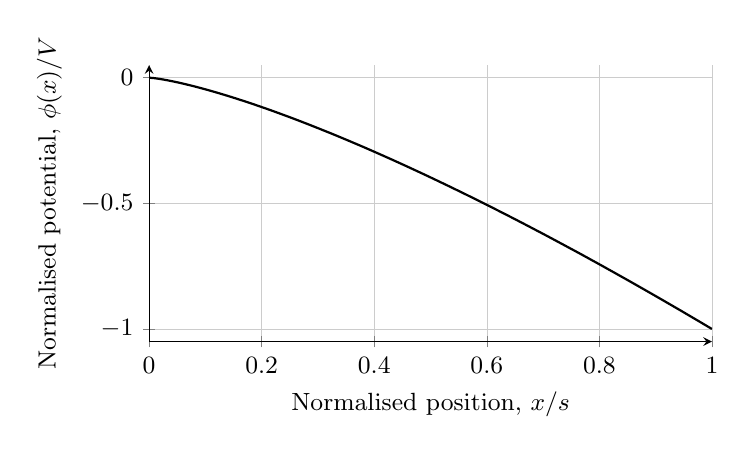
\begin{tikzpicture}
\begin{axis}[
 width=0.72\linewidth,
 height=0.42\linewidth,
 xlabel={Normalised position, $x/s$},
 ylabel={Normalised potential, $\phi(x)/V$},
 xmin=0, xmax=1,
 ymin=-1.05, ymax=0.05,
 domain=0:1,
 samples=100,
 axis lines=left,
 grid=both,
 grid style={line width=0.1pt, draw=gray!30},
 major grid style={line width=0.2pt, draw=gray!40},
 tick label style={font=\small},
 label style={font=\small},
 every axis plot/.append style={thick, black},
]
\addplot[black, thick] {-(x)^(4/3)};
\end{axis}
\end{tikzpicture}
\caption{Schematic potential profile of a planar, space-charge-limited (Child--Langmuir) sheath, plotted from the analytic law $\phi(x)/V=-(x/s)^{4/3}$ of Eq.~\eqref{eq:cl-profile}. No measured or simulated data are represented; the curve illustrates only the characteristic concave shape of the fluid-model sheath potential.}
\label{fig:cl-profile}
\end{figure}

\subsection{Where the fluid description breaks down}
\label{sec:breakdown}

The fluid sheath model is bounded by the same considerations as any truncated moment hierarchy: reliable when $f_{\mathrm{i}}(v)$ is sharply peaked and single-valued at each $x$, degrading when the distribution broadens, becomes multi-valued, or acquires trapped/reflected particles a single fluid velocity $u_{\mathrm{i}}(x)$ cannot represent. Four mechanisms drive this breakdown.

First, ions are not mono-energetic even at the sheath edge: born by ionisation across a spread of positions and accelerated by different potential drops, $f_{\mathrm{i}}(v)$ is a superposition with finite spread rather than a delta function. The Tonks--Langmuir kinetic model shows this spread is intrinsic to the collisionless presheath and irremovable by any scalar closure \cite{ref0665,ref0666}; the kinetic Bohm criterion, an integral condition on $f_{\mathrm{i}}(v)$, reduces to the fluid result only in the cold-beam limit and can differ materially near $v\to0$. Second, the density profile of Eq.~\eqref{eq:ni-of-phi} diverges as $u_{\mathrm{i}}(x)\to0$, avoided only because Eq.~\eqref{ch12-eq:bohm-criterion} guarantees $u_{\mathrm{i}}\ge u_{\mathrm{B}}>0$; a kinetic treatment instead lets the low-velocity tail vanish smoothly. Third, in magnetised or grazing-angle configurations ion gyromotion introduces velocity components a scalar or tensor closure captures only approximately; the Chodura magnetic presheath, acting over the ion gyroradius rather than the Debye length, is a multi-scale phenomenon fluid models reproduce only coarsely \cite{ref0017,ref0018}. Fourth, and most relevant here, the high-energy tail of the ion energy distribution — which sets sputtering-yield thresholds and etch/erosion-rate curves — is controlled by ions with atypical histories, invisible to a single-velocity cold-fluid closure, and needs either a fully kinetic solution or a fluid model augmented with a modelled energy spread \cite{ref0083}. Continuum-kinetic comparisons confirm the mean ion flux and leading Bohm moment are reproduced accurately by the fluid model, while higher moments — the energy-flux-weighted tail especially — deviate systematically as the ion thermal spread grows relative to the directed sheath-edge velocity \cite{ref0659}. In collisional or non-Maxwellian discharges, charge exchange repopulates low-energy ions throughout the sheath, producing a bimodal $f_{\mathrm{i}}(v)$ no single fluid velocity can represent without a multi-population closure \cite{ref0077,ref0090}.

\section{Boundary Conditions at the Sheath Edge}
\label{sec:bc}

\subsection{The Bohm criterion as a boundary condition}

In practice, the fluid sheath equations of Sec.~\ref{sec:sheath-models} are coupled to a quasineutral presheath solution from Sec.~\ref{sec:closure}, matched at a nominal "sheath edge." The Bohm criterion, Eq.~\eqref{ch12-eq:bohm-criterion}, is the boundary condition imposed there: the presheath must deliver ions with fluid velocity no smaller than $c_{\mathrm{s}}=\sqrt{T_{\mathrm{e}}/m_{\mathrm{i}}}$. The marginal equality is normally adopted, since the presheath field self-consistently accelerates ions to exactly $u_{\mathrm{B}}=c_{\mathrm{s}}$ where quasineutrality first fails; this is imposed as a Dirichlet-type velocity condition in essentially all fluid sheath codes.

\subsection{Generalised forms of the boundary condition}

Equation~\eqref{ch12-eq:bohm-criterion} generalises in several directions relevant to realistic discharges.

\begin{itemize}
\item \textbf{Warm and polytropic ions.} A finite ion temperature at the sheath edge raises the required entry speed to $u_{\mathrm{B}}=\sqrt{(T_{\mathrm{e}}+\gamma_{\mathrm{i}}T_{\mathrm{i}0})/m_{\mathrm{i}}}$ (Table~\ref{tab:closures}), applied as the boundary condition.
\item \textbf{Multiple ion species.} With two or more positive ion species of different mass, the criterion becomes an inequality on a weighted sum, $\sum_j n_{j}T_{\mathrm{e}}/(m_ju_j^2) \le n_{\mathrm{e}}$, so a light species may enter below its own sound speed if a heavier one compensates; individual boundary velocities need an auxiliary closure.
\item \textbf{Magnetised sheaths.} For a field inclined at angle $\alpha$ to the wall, the Bohm--Chodura condition requires the ion velocity along $\mathbf{B}$ to reach $c_{\mathrm{s}}$ at the magnetic presheath entrance, and the wall-normal component to satisfy the ordinary Bohm criterion at the thinner electrostatic sheath edge — two conditions at two distinct boundaries \cite{ref0017,ref0018}.
\item \textbf{Non-Maxwellian electrons.} If electrons deviate from Maxwellian, Eq.~\eqref{eq:boltzmann-electrons} no longer holds, and the boundary condition must be re-derived from the actual electron energy distribution, generally yielding a different coefficient in place of $\sqrt{T_{\mathrm{e}}/m_{\mathrm{i}}}$ \cite{ref0090}.
\end{itemize}

\subsection{Quasineutral matching and the presheath}

Formally, Eq.~\eqref{ch12-eq:bohm-criterion} is a marginal-stability condition on the quasineutral presheath solution, and the sheath itself is a boundary layer of thickness $\mathcal{O}(\lambda_{\mathrm{D}})$, thin compared with the presheath scale $\mathcal{O}(L)$. Matched-asymptotic treatments confirm the quasineutral presheath and non-neutral sheath equations can be solved as two separate problems, joined by continuity of $n_{\mathrm{i}}$, $u_{\mathrm{i}}$ and $\phi$ at the matching layer, with the Bohm criterion emerging as the solvability condition rather than an additional postulate. This is why a practical sheath code can patch a quasineutral drift-diffusion solution for the bulk onto a collisionless space-charge solution for the sheath, without resolving Debye-scale physics everywhere \cite{ref0012}.

\subsection{Practical implementation in fluid codes}

Three essentially equivalent implementations are common. The simplest fixes the ion fluid velocity at the last quasineutral grid point to the local sound speed, $u_{\mathrm{i}} = c_{\mathrm{s}}$, and integrates the sheath equations outward, adequate whenever the presheath solution is smooth. The second imposes a sonic outflow condition on the presheath drift-diffusion equation, letting the solution select where $u_{\mathrm{i}}$ first reaches $c_{\mathrm{s}}$, more self-consistent for non-planar geometries \cite{ref0013}. The third, used in particle and hybrid codes, replaces the sharp Bohm condition with a "logical sheath" or absorbing boundary that removes particles crossing a nominal wall and infers the sheath potential from the resulting charge imbalance, trading analytic transparency for validity when $f_{\mathrm{i}}(v)$ is not well approximated by a single fluid velocity (Sec.~\ref{sec:breakdown}) \cite{ref0659}. In all three, the presheath equations are solved up to where Eq.~\eqref{ch12-eq:bohm-criterion} is saturated, and the Sec.~\ref{sec:sheath-models} sheath solution is launched with $u_{\mathrm{i}}=u_{\mathrm{B}}$, $n_{\mathrm{i}}=n_{\mathrm{e}}=n_0$, $\phi=0$.

\section{Utility for Fast Forward Modelling in the Inversion}
\label{sec:forward}

\subsection{The computational cost hierarchy}

The inversion problem addressed by this monograph — recovering bulk plasma parameters ($n_0$, $T_{\mathrm{e}}$, and the sheath voltage or bias waveform) from a measured or targeted ion energy flux $\Gamma_E$ — requires a forward model evaluable an enormous number of times: once per proposal in a Markov-chain Monte Carlo sampler, once per grid-search combination, or once per optimiser iteration. Candidate forward models span many orders of magnitude in cost. A fully kinetic solution of Eq.~\eqref{ch12-eq:boltzmann} — by Vlasov discretisation, discontinuous-Galerkin methods, or particle-in-cell simulation with Monte Carlo collisions — requires resolving both the Debye length and electron plasma period, scaling unfavourably with the mass ratio $m_{\mathrm{i}}/m_{\mathrm{e}}$ and phase-space dimensionality. Continuum-kinetic solvers, though far more accurate than fluid models in the regimes of Sec.~\ref{sec:breakdown}, remain orders of magnitude more expensive per evaluation \cite{ref0659,ref0665,ref0666}. A single such solve, run once for validation, is tractable; running it inside an inversion with thousands to millions of calls is not.

\subsection{Semi-analytic ion energy flux from the fluid closure}

The fluid sheath model reduces the forward problem to evaluating a small number of closed-form or low-order-ODE expressions. Given $(n_0, T_{\mathrm{e}}, T_{\mathrm{i}0}, V_{\text{sheath}})$, the Bohm velocity follows from Table~\ref{tab:closures}; the sheath-edge flux from $\Gamma_{\mathrm{i}} = n_0u_{\mathrm{B}}$; and, in the cold-ion approximation, the ion energy flux at the wall from energy conservation along Eq.~\eqref{eq:ion-energy-cons} evaluated at $\phi=-V_{\text{sheath}}$,
\begin{equation}
\Gamma_E \simeq n_0u_{\mathrm{B}}\left(\tfrac{1}{2}m_{\mathrm{i}}u_{\mathrm{B}}^2 + eV_{\text{sheath}}\right),
\label{eq:GammaE-forward}
\end{equation}
a single algebraic expression, evaluable to machine precision in microseconds, replacing what would otherwise be a full kinetic transport calculation. Where the Child--Langmuir limit applies instead ($eV_{\text{sheath}}\gg T_{\mathrm{e}}$), Eq.~\eqref{ch12-eq:child-langmuir} gives an equally compact relation between voltage, sheath thickness and ion current density, from which $\Gamma_E \simeq J_{\mathrm{i}}V_{\text{sheath}}$ follows directly. Both expressions are low-order power laws, trivially differentiable in closed form, requiring no discretisation, mesh, or time-stepping.

\subsection{Role in the inversion workflow}

This monograph uses the fluid forward model of Eq.~\eqref{eq:GammaE-forward}, or its Child--Langmuir counterpart, as the workhorse evaluated inside the inversion loop, reserving kinetic or hybrid solves for a sparse set of validation points bounding the systematic error the closure introduces. This two-tier strategy is standard wherever cost asymmetry precludes a purely kinetic inversion: fast, closed-form fluid or power-balance relations serve parameter scans \cite{ref0093}, while more expensive models supply local corrections at limited anchor points. The bias from the cold-fluid closure — chiefly neglect of the ion energy spread (Sec.~\ref{sec:breakdown}) — can be partly compensated within the fluid framework by an energy-spectrum-resolved closure \cite{ref0083}, retaining a fluid solve's speed while approximating the leading kinetic correction. The fluid model of this chapter is thus not merely a pedagogical simplification but the load-bearing engine that makes a many-evaluation inversion of the ion energy flux problem feasible.

\section{Summary}

This chapter developed the fluid description of plasmas and sheaths as a systematic truncation of the moment hierarchy of the Boltzmann equation. The zeroth, first and second velocity moments gave continuity, momentum and energy equations~\eqref{eq:continuity}--\eqref{eq:energy}, an open hierarchy requiring an explicit closure. Cold, isothermal and polytropic pressure closures, the drift-diffusion reduction for collisional bulk plasmas, and the two-fluid model coupling ions and electrons through Poisson's equation were compared in Table~\ref{tab:closures}. The cold-ion, Boltzmann-electron closure applied to the collisionless planar sheath yielded the governing equation~\eqref{eq:sheath-ode}, from which the Bohm criterion, Eq.~\eqref{ch12-eq:bohm-criterion}, was derived by linear stability and the Sagdeev pseudopotential method, and the Child--Langmuir law, Eq.~\eqref{ch12-eq:child-langmuir}, obtained as the strongly biased limit. The Bohm criterion was then examined as the boundary condition coupling the quasineutral presheath to the non-neutral sheath, in its warm-ion, multi-species and magnetised generalisations, with practical implementation in fluid codes outlined. The chapter identified where the single-fluid-velocity closure breaks down — energy spread at the sheath edge, the apparent field singularity, magnetic presheath structure, and the high-energy distribution-function tail — and where a kinetic or hybrid treatment is necessary. Finally, via the closed-form Eq.~\eqref{eq:GammaE-forward}, it argued that reducing a phase-space kinetic problem to a handful of algebraic relations is what makes the fluid sheath model the appropriate forward operator for a many-evaluation inversion of ion energy flux measurements, with kinetic corrections retained only where Sec.~\ref{sec:breakdown} shows them necessary.

\chapter{Kinetic Theory and Particle-in-Cell Simulation}
\label{ch:pic}

The fluid and hybrid treatments developed in preceding chapters close the ion and electron moment equations with assumptions --- a cold or warm mono-energetic ion beam, a Boltzmann electron response, a prescribed collisionality --- that are convenient but not always defensible at the plasma--sheath boundary. The Bohm criterion is, at root, a statement about the low-velocity tail of the ion distribution function, and the ion energy flux $\Gamma_{E}$ this monograph seeks to quantify is an integral over that distribution weighted by kinetic energy. Whenever $f_{\mathrm{i}}(v)$ departs materially from a drifting Maxwellian --- because of a collisionless presheath, a time-varying sheath edge, a non-Maxwellian electron population, or an oblique magnetic field --- a moment-based closure can misrepresent both the total flux and the energy-resolved spectrum a retarding-field or laser diagnostic actually records. This chapter develops the kinetic description of the plasma--wall system from first principles, introduces the particle-in-cell (PIC) method as the primary tool for the self-consistent sheath problem, and explains how PIC-generated data construct synthetic ground truth for validating later inversion algorithms. It closes with the computational cost of kinetic simulation and a survey of reduced kinetic models that make routine sheath-diagnostic work tractable without discarding the physics fluid closures wash out.

\section{The Vlasov and Boltzmann Descriptions}

\subsection{Phase-space distribution functions and the kinetic equation}

The most complete non-relativistic description of a plasma species $s$, short of following every particle trajectory, is the one-particle distribution function $f_{s}(\mathbf{r},\mathbf{v},t)$, defined such that $f_{s}(\mathbf{r},\mathbf{v},t)\,\mathrm{d}^{3}r\,\mathrm{d}^{3}v$ is the expected particle count in the phase-space element at $(\mathbf{r},\mathbf{v})$ at time $t$. All fluid quantities used elsewhere in this monograph are low-order velocity moments of $f_{s}$:
\begin{align}
n_{s}(\mathbf{r},t) &= \int f_{s}(\mathbf{r},\mathbf{v},t)\,\mathrm{d}^{3}v, \\
n_{s}\mathbf{u}_{s}(\mathbf{r},t) &= \int \mathbf{v}\, f_{s}(\mathbf{r},\mathbf{v},t)\,\mathrm{d}^{3}v, \\
p_{s}(\mathbf{r},t) &= \frac{m_{s}}{3}\int |\mathbf{v}-\mathbf{u}_{s}|^{2} f_{s}(\mathbf{r},\mathbf{v},t)\,\mathrm{d}^{3}v = n_{s} T_{s},
\end{align}
with $T_{\mathrm{e}}$ and $T_{\mathrm{i}}$ the electron and ion temperatures used throughout this work. In the absence of collisions, $f_s$ obeys the Vlasov equation, expressing conservation of phase-space density along single-particle trajectories in the self-consistent field:
\begin{equation}
\frac{\partial f_{s}}{\partial t} + \mathbf{v}\cdot\nabla_{\mathbf{r}} f_{s} + \frac{q_{s}}{m_{s}}\left(\mathbf{E} + \mathbf{v}\times\mathbf{B}\right)\cdot\nabla_{\mathbf{v}} f_{s} = 0,
\label{eq:vlasov}
\end{equation}
where $q_{s}$, $m_{s}$ are charge and mass, and $\mathbf{E}$, $\mathbf{B}$ are determined self-consistently from Maxwell's equations (or, in the electrostatic limit relevant to most sheath problems, from Poisson's equation with charge densities given by the zeroth moment of $f_{s}$). Equation~\eqref{eq:vlasov} is linear and hyperbolic; the non-linearity of the plasma problem enters entirely through the coupling of $\mathbf{E}$, $\mathbf{B}$ back to the moments of $f_{s}$ \cite{ref0670}. It is collisionless, an approximation justified whenever the number of particles within a Debye sphere, $N_{\mathrm{D}} = \tfrac{4}{3}\pi n_{\mathrm{e}} \lambda_{\mathrm{D}}^{3}$, is large, so two-body encounters contribute negligibly to the mean-field dynamics.

When binary collisions are not negligible, the right-hand side of Eq.~\eqref{eq:vlasov} acquires a collision operator, yielding the Boltzmann equation,
\begin{equation}
\frac{\partial f_{s}}{\partial t} + \mathbf{v}\cdot\nabla_{\mathbf{r}} f_{s} + \frac{q_{s}}{m_{s}}\left(\mathbf{E} + \mathbf{v}\times\mathbf{B}\right)\cdot\nabla_{\mathbf{v}} f_{s} = \left(\frac{\partial f_{s}}{\partial t}\right)_{\!\mathrm{coll}},
\label{ch13-eq:boltzmann}
\end{equation}
with the collision term written, for elastic binary encounters, in the classical Boltzmann integral form with differential cross-section $\sigma(\mathbf{v},\mathbf{v}';\Omega)$, or, for small-angle Coulomb scattering, in the Fokker--Planck (Landau) form \cite{ref0670}. Both equations are exact conservation statements; the physics of a kinetic model lies entirely in the choice of collision operator, or its omission.

\subsection{Moments, closure, and the failure of fluid models near boundaries}

Multiplying Eq.~\eqref{ch13-eq:boltzmann} by successive powers of $\mathbf{v}$ and integrating generates the familiar hierarchy of fluid moment equations, but each contains a flux term equal to the next-higher moment, so the $n$-th equation always involves an unknown $(n+1)$-th moment. Fluid models close this hierarchy by asserting a relationship between the unclosed moment and lower ones: an equation of state, a Fourier-law heat flux, or, in the cold-ion models used earlier in this monograph, a delta-function or drifting-Maxwellian ion distribution. Such closures are excellent deep in the quasi-neutral bulk, where collisions or turbulent scattering keep $f_{s}$ near local equilibrium.

The closure fails wherever $f_s$ develops structure a low-order moment cannot represent. Three failure modes are of direct relevance to sheath physics:

\begin{enumerate}
\item \textbf{Presheath acceleration without local equilibration.} Ions born at rest are accelerated continuously through the presheath field. If the ion mean free path exceeds the presheath length scale, ions never re-thermalise; the sheath-edge distribution is a strongly non-Maxwellian, one-sided function set by the entire accelerating history, not a local temperature \cite{ref0665,ref0666,ref0659}. This is the regime of the kinetic Tonks--Langmuir model, where the kinetic Bohm criterion --- an inequality on the low-velocity moment of $f_{\mathrm{i}}(v)$, not a fluid drift-speed condition --- must be invoked.
\item \textbf{Trapped and reflected populations.} Electrons (and, in reversing or double-layer sheaths, ions) can be partially reflected, producing a sharp velocity-space cutoff at the local escape energy that a smooth closure cannot represent, but that emerges naturally from the collisionless solution of Eq.~\eqref{eq:vlasov} \cite{ref0670}.
\item \textbf{Non-stationary or oscillating boundaries.} In RF-driven and pulsed sheaths the edge moves on a timescale comparable to, or shorter than, the ion transit time, so the instantaneous distribution superposes sub-populations entering the presheath at different drive phases --- an object no single-temperature closure can capture \cite{ref0637}.
\end{enumerate}

\subsection{When kinetic effects matter: a practical Knudsen-type criterion}

A convenient way to decide whether a fully kinetic treatment is required is to compare the relevant collisional mean free path $\lambda_{\mathrm{mfp}}$ (ion--neutral charge exchange, ion--ion Coulomb scattering, electron--neutral excitation) with the length scale over which the distribution is formed, typically the presheath length $L_{\mathrm{ps}}$:
\begin{equation}
\mathrm{Kn} = \frac{\lambda_{\mathrm{mfp}}}{L_{\mathrm{ps}}}.
\end{equation}
For $\mathrm{Kn} \gg 1$ transport is collisionless and a kinetic treatment is mandatory for energy-resolved quantities such as $\Gamma_{E}$, even though fluid moments like $n_{\mathrm{i}}$ and $u_{\mathrm{i}}$ may remain tolerably accurate. For $\mathrm{Kn}\ll 1$ a corrected fluid closure is usually adequate for the flux itself, though the tail can still deviate since it is populated by the least-collided particles \cite{ref0672}. The intermediate regime $\mathrm{Kn}\sim 1$, common near \SI{1}{\pascal}, is where kinetic simulation is most valuable and analytic theory becomes intractable.

\section{The Particle-in-Cell Method}

\subsection{Superparticles and the discretisation of phase space}

Direct solution of Eq.~\eqref{eq:vlasov} or \eqref{ch13-eq:boltzmann} on a phase-space grid --- the continuum (Eulerian) approach --- is possible, but resolving up to six dimensions is prohibitive for routine scans. PIC instead represents $f_{s}$ as a finite sum of computational \emph{superparticles}, each with a weight $w_{p}$ standing in for many physical particles sharing the same position and velocity:
\begin{equation}
f_{s}(\mathbf{r},\mathbf{v},t) \approx \sum_{p=1}^{N_{p}} w_{p}\, S(\mathbf{r}-\mathbf{r}_{p}(t))\, \delta(\mathbf{v}-\mathbf{v}_{p}(t)),
\end{equation}
where $S$ is a finite-support shape function (commonly linear, ``cloud-in-cell'') that spreads each particle's contribution over neighbouring grid nodes. This converts phase-space transport into the cheaper problem of advancing $N_{p}$ particle-orbit ODEs coupled to a field solve on a spatial grid of far lower dimensionality. Statistical noise from representing smooth $f$ by finite markers scales as $1/\sqrt{N_{p}}$ per cell: more particles reduce noise but raise cost linearly, so particles-per-Debye-length-cell must be chosen with the same care as grid spacing.

\subsection{The PIC cycle: weighting, field solve, force interpolation, particle push}

A single PIC time step advances the system through four operations, per species per step:

\begin{enumerate}
\item \textbf{Charge weighting.} Each superparticle's charge $q_{s}w_{p}$ is deposited onto nearby grid nodes using the shape function $S$ used for force interpolation (avoiding a spurious self-force), giving a grid charge density $\rho(\mathbf{r}_{i})$.
\item \textbf{Field solve.} Poisson's equation (electrostatic PIC, appropriate for most low-temperature sheath problems) or the full Maxwell system is solved on the grid,
\begin{equation}
\nabla^{2}\phi(\mathbf{r}) = -\frac{\rho(\mathbf{r})}{\varepsilon_{0}}, \qquad \mathbf{E}(\mathbf{r}) = -\nabla \phi(\mathbf{r}),
\label{ch13-eq:poisson}
\end{equation}
using a direct or iterative linear solver.
\item \textbf{Force interpolation (gather).} The grid field $\mathbf{E}(\mathbf{r}_{i})$ (and $\mathbf{B}(\mathbf{r}_{i})$ if present) is interpolated back to each particle's position using $S$.
\item \textbf{Particle push.} Position and velocity are advanced by the Lorentz force equation,
\begin{equation}
\frac{\mathrm{d}\mathbf{v}_{p}}{\mathrm{d}t} = \frac{q_{s}}{m_{s}}\left(\mathbf{E}(\mathbf{r}_{p}) + \mathbf{v}_{p}\times\mathbf{B}(\mathbf{r}_{p})\right), \qquad \frac{\mathrm{d}\mathbf{r}_{p}}{\mathrm{d}t} = \mathbf{v}_{p}.
\label{eq:lorentz}
\end{equation}
\end{enumerate}
This weight--solve--gather--push cycle is the discrete analogue of Vlasov--Poisson; its self-consistency --- the field pushing the particles is generated by those particles' own charge density --- makes PIC a genuinely non-linear kinetic solver rather than a test-particle tracer in a fixed field. Foundational applications showed that a fully kinetic, self-consistent simulation reproduces the Bohm-criterion-satisfying presheath and sheath potential profile without any fluid closure \cite{ref0631}, and the method has since been applied to planar, magnetized, and pulsed sheath geometries \cite{ref0633}.

\subsection{Time integration: the Boris algorithm and leapfrog scheme}

The particle push is almost universally integrated using the leapfrog scheme, positions at integer levels $t^{n}$ and velocities at half-integer levels $t^{n+1/2}$:
\begin{align}
\mathbf{r}_{p}^{n+1} &= \mathbf{r}_{p}^{n} + \mathbf{v}_{p}^{n+1/2}\,\Delta t, \\
\mathbf{v}_{p}^{n+1/2} &= \mathbf{v}_{p}^{n-1/2} + \frac{q_{s}\Delta t}{m_{s}}\left(\mathbf{E}_{p}^{n} + \frac{\mathbf{v}_{p}^{n+1/2}+\mathbf{v}_{p}^{n-1/2}}{2}\times\mathbf{B}_{p}^{n}\right).
\end{align}
The magnetic-rotation term, implicit in the velocity average, is solved non-iteratively by the Boris rotation: the electric acceleration is split into two half-steps bracketing an exact, energy-conserving rotation about $\mathbf{B}_{p}^{n}$. The scheme is only second-order accurate but symplectic, introducing no secular energy drift over the $10^{4}$--$10^{6}$ steps typical of a sheath run, which is why it remains standard even in modern implicit and magnetized codes \cite{ref0637}. In magnetized sheaths, where the gyro-period can be the fastest timescale, the push must additionally resolve cyclotron rotation, $\Omega_{c}\Delta t \lesssim 0.2$ ($\Omega_{c}=qB/m$), alongside the electrostatic constraints below \cite{ref0633,ref0637}.

\subsection{Stability and accuracy: CFL, Debye-length resolution, and finite-grid instability}

Explicit electrostatic PIC is subject to three coupled stability requirements that jointly determine $\Delta x$, $\Delta t$, and superparticles per Debye-length cell.

\paragraph{CFL condition.} No particle may cross more than one cell per step:
\begin{equation}
\Delta t \le \frac{\Delta x}{v_{\max}},
\end{equation}
with $v_{\max}$ the fastest particle speed present.

\paragraph{Plasma-period resolution.} The explicit leapfrog scheme is unstable, independent of CFL, if the electron plasma oscillation is not resolved in time:
\begin{equation}
\omega_{\mathrm{pe}}\,\Delta t \lesssim 0.2,
\qquad
\omega_{\mathrm{pe}} = \sqrt{\frac{n_{\mathrm{e}} e^{2}}{\varepsilon_{0} m_{\mathrm{e}}}}.
\label{eq:wpe_dt}
\end{equation}
This is usually the most restrictive condition for dense, low-temperature discharges: a typical run ($n_{\mathrm{e}}\sim\SI{e16}{\per\cubic\metre}$) requires order $10^{5}$--$10^{6}$ steps merely to reach one ion transit time across the presheath.

\paragraph{Debye-length grid resolution and finite-grid instability.} The grid must resolve the electron Debye length,
\begin{equation}
\Delta x \lesssim \lambda_{\mathrm{D}}, \qquad \lambda_{\mathrm{D}} = \sqrt{\frac{\varepsilon_{0} T_{\mathrm{e}}}{n_{\mathrm{e}} e^{2}}},
\end{equation}
with a practical guideline $\Delta x \le (0.5\text{--}1)\,\lambda_{\mathrm{D}}$. If violated, the discrete Poisson solver aliases short-wavelength fluctuations onto long wavelengths, producing a spurious \emph{finite-grid instability} that artificially heats electrons and can distort the presheath structure. Because the sheath is only a few $\lambda_{\mathrm{D}}$ thick, resolving it while also resolving the much larger bulk on a uniform grid can be demanding, motivating non-uniform and curvilinear grids. The particles-per-cell count, $N_{\mathrm{ppc}}$, controls statistical noise in derived quantities such as $\Gamma_{E}$; since relative fluctuation scales as $N_{\mathrm{ppc}}^{-1/2}$, resolving the tail of $f_{\mathrm{i}}(v)$, where $v^{2}$ or $v^{3}$ weighting places most statistical weight, typically needs one to two orders of magnitude more particles per cell than resolving density alone. Table~\ref{tab:pic_stability} summarises these constraints.

\begin{table}[htbp]
\centering
\caption{Principal stability and resolution constraints for explicit electrostatic PIC simulation of a plasma sheath. Quantities are defined in the main text; numerical prefactors are conventional guidelines, not sharp bounds.}
\label{tab:pic_stability}
\begin{tabularx}{\linewidth}{@{}l X l@{}}
\toprule
Constraint & Physical origin & Typical form \\
\midrule
Time-step / plasma period & Explicit leapfrog stability of electron plasma oscillation & $\omega_{\mathrm{pe}}\Delta t \lesssim 0.2$ \\
Time-step / cyclotron period & Accurate resolution of gyromotion in magnetized sheaths & $\Omega_{c}\Delta t \lesssim 0.2$ \\
Time-step / CFL & Particle must not skip a cell per step & $\Delta t \le \Delta x / v_{\max}$ \\
Grid spacing / Debye length & Avoidance of finite-grid (aliasing) heating instability & $\Delta x \lesssim (0.5\text{--}1)\lambda_{\mathrm{D}}$ \\
Particles per cell & Control of statistical noise in $f_{\mathrm{i}}(v)$ and its moments & $N_{\mathrm{ppc}} \gtrsim 10^{2}\text{--}10^{3}$ \\
\bottomrule
\end{tabularx}
\end{table}

\subsection{Boundary conditions at plasma-facing surfaces}

Wall-boundary treatment most distinguishes a sheath-oriented PIC code from a generic bounded-plasma solver. At minimum, an absorbing boundary removes a particle the instant it crosses the wall and deposits its charge there (or in a circuit model, for a floating or capacitively coupled electrode); the accumulated wall charge and bias set the boundary condition for the Poisson solve, Eq.~\eqref{ch13-eq:poisson}. More complete models add secondary electron emission, energy- and angle-dependent reflection, and, for dielectric walls, an accumulating surface-charge density --- effects that alter the sheath potential drop and reflected electron component, and require care to avoid spurious charge non-conservation. This is not a bookkeeping detail: since $\Gamma_{E}$ is evaluated at the wall, any boundary error propagates directly into the synthetic ground-truth spectra used for inversion validation in Section~\ref{sec:synthetic_ground_truth}, and naive treatments introduce spurious low-energy structure in the recorded ion distribution.

\section{Collisions in PIC: Monte Carlo Methods and DSMC Coupling}

\subsection{The null-collision Monte Carlo collision (MCC) algorithm}

Collisions between charged and neutral species are incorporated into an otherwise collisionless PIC push through a Monte Carlo collision (MCC) module, interleaved with the PIC cycle (PIC-MCC). For a uniform, stationary neutral gas of density $n_{\mathrm{n}}$, the probability that a superparticle of speed $v$ undergoes process $k$ (elastic scattering, excitation, ionisation, charge exchange, \ldots) in one step is
\begin{equation}
P_{k}(v) = 1 - \exp\!\big[-n_{\mathrm{n}}\,\sigma_{k}(v)\,v\,\Delta t\big] \approx n_{\mathrm{n}}\,\sigma_{k}(v)\,v\,\Delta t,
\end{equation}
with $\sigma_{k}(v)$ the cross-section. Testing this for every particle and process every step is wasteful; the standard solution is the \emph{null-collision method}, in which a single maximum collision frequency
\begin{equation}
\nu_{\max} = n_{\mathrm{n}}\max_{v}\Big[v\sum_{k}\sigma_{k}(v)\Big]
\end{equation}
sets a fixed total probability $P_{\mathrm{null}}=1-\exp(-\nu_{\max}\Delta t)$; a random subset of particles is selected as candidates, and a second, cross-section-weighted draw decides which process (if any) occurs. This reduces cost from $O(N_{p}\times N_{\mathrm{processes}})$ to $O(N_{p})$ evaluations and is used in essentially all PIC-MCC codes for low-temperature sheath problems \cite{ref0637}. Post-collision velocities are sampled from the relevant cross-section, and ionising collisions create a new electron--ion pair with partitioned energy and momentum.

\subsection{Direct simulation Monte Carlo and its coupling to PIC}

MCC treats the neutral background as a fixed reservoir --- valid when ionisation is low and the gas only weakly heated or depleted. When neutral heating, rarefaction, or strong charge-exchange coupling must be captured self-consistently, the neutral gas is instead represented kinetically via direct simulation Monte Carlo (DSMC): neutral superparticles advance ballistically between cells and undergo binary collisions with a partner drawn stochastically from the same cell, at a rate set by a null-collision scheme. Coupling PIC (charged species) to DSMC (neutrals) lets charge-exchange and elastic ion--neutral collisions modify the neutral distribution self-consistently, which matters where resonant charge exchange dominates ion loss: a fast ion can charge-exchange with a slow neutral, instantly replacing a high-energy trajectory with a near-thermal one and populating a distinct low-energy sub-population in $f_{\mathrm{i}}(v)$ at the sheath edge. Multispecies simulations of the hydrogen plasma sheath, tracking several ionic species and their charge-exchange partners, illustrate the practical importance of resolving this structure kinetically rather than through a single-fluid closure. PIC/test-particle schemes, where a self-consistent PIC-MCC bulk solution provides fields and rates for a separately tracked ensemble of sputtered particles, extend this coupling to transport away from a surface.

\subsection{Coulomb collisions and binary collision models}

Long-range Coulomb interactions are formally already contained in the mean-field Vlasov term insofar as the PIC grid resolves the corresponding wavelengths, but graininess of the finite-$N_{p}$ representation introduces artificial collisionality unless $N_{\mathrm{ppc}}$ is large; capturing the correct small-angle Coulomb scattering rate requires an explicit binary Coulomb-collision (Takizuka--Abe-type) module drawing partners from the same spatial cell. Because Coulomb rates scale steeply with relative velocity ($\propto v^{-3}$), such modules matter for thermalisation of the fast electron tail and for ion--ion collisions reshaping the ion velocity distribution near the sheath edge under instability-enhanced collisionality.

\section{Particle-in-Cell Simulation of Plasma Sheaths}

\subsection{Non-Maxwellian ion and electron tails at the sheath edge}

Kinetic PIC simulation of the collisionless plasma--sheath transition consistently reproduces non-Maxwellian features fluid theory cannot: a low-velocity ion population depleted relative to a Maxwellian (the slowest ions are most efficiently accelerated out of the presheath, a self-selection effect at the heart of the kinetic Bohm criterion \cite{ref0665,ref0666}); a high-velocity tail set by the total presheath potential drop rather than a thermal speed; and a truncated electron distribution from preferential loss of the fastest electrons to the wall, partially compensated by secondary-electron re-emission. Fully kinetic simulations were among the first to demonstrate that the sheath-edge ion distribution satisfies the kinetic Bohm criterion in its integral, not simplified fluid, form, and that the low-velocity tail's shape, not merely its second moment, controls marginal stability \cite{ref0631}. Subsequent studies extended this to magnetized sheaths, where the ion distribution acquires structure from gyromotion projected onto the wall normal and from the Chodura-layer transition preceding the Debye sheath \cite{ref0633,ref0637}.

A further class of non-Maxwellian structure arises from multi-species plasmas. Ion--ion plasma simulations (electronegative discharges, or plasmas with two positive-ion species) show each species developing its own sheath-edge velocity distribution, the lighter species dominating the low-energy portion of the combined flux spectrum and the heavier contributing a sharper peak \cite{ref0655}. Because an inversion algorithm recovering $T_{\mathrm{e}}$, $n_{\mathrm{e}}$, or a sheath-potential waveform implicitly assumes a functional form for $f_{\mathrm{i}}(v)$, quantifying how far a PIC-computed distribution departs from that form is a principal diagnostic use of kinetic simulation.

\subsection{Transient and RF-driven sheath dynamics}

RF and pulsed sources present a qualitatively distinct problem: the sheath edge, and hence the instantaneous accelerating potential, oscillates on a timescale that, for typical drive frequencies (\SIrange{1}{100}{\mega\hertz}), can range from much slower than to faster than the ion transit time. When transit time greatly exceeds the RF period, ions respond only to the time-averaged potential and the energy distribution collapses toward a narrow, quasi-mono-energetic peak; when the two periods are comparable, ions respond to the instantaneous field and the distribution broadens into the bimodal structure long observed in capacitively coupled discharges. PIC is the natural tool for this intermediate regime, tracking each ion's transit history without assuming which limit applies \cite{ref0637}, providing the basis for interpreting retarding-field and mass-spectrometric IEDF measurements \cite{ref0672}.

Two further transients are captured naturally by PIC but essentially inaccessible to a fluid closure. Sheath collapse and reversal --- a rapidly changing bias driving the sheath potential briefly below floating or momentarily positive, permitting a transient electron flux before the sheath re-forms --- requires tracking the full evolving distribution rather than a steady-state moment. The finite relaxation time of the presheath and Chodura-layer structures after a step change in bias or plasma parameters --- the ``formation transient'' --- itself carries diagnostic information about collisionality and ion mass.

\subsection{Synthetic diagnostics extracted from PIC}

A PIC simulation stores, at every step, the full six-dimensional (or reduced 1D3V) phase-space information for every superparticle, making it straightforward to construct \emph{synthetic diagnostics} --- numerically evaluated analogues of a real instrument's response --- essential for closing the loop between kinetic theory and the inversion methodology developed later. Three recur throughout:

\begin{itemize}
\item \textbf{Synthetic retarding-field analyser (RFA) trace.} Ions crossing a virtual detector plane are binned by wall-normal kinetic energy and convolved with the same instrument response function (grid transmission, energy resolution, space-charge-limited transmission) used to interpret an experimental trace.
\item \textbf{Synthetic laser-induced-fluorescence (LIF) spectrum.} A Doppler-resolved velocity-space slice extracted from stored superparticle velocities and convolved with natural and instrumental linewidths, directly comparable with measured ion velocity distributions.
\item \textbf{Synthetic mass-spectrometric IEDF.} Superparticles are additionally binned by mass-to-charge ratio prior to energy binning, reproducing the joint energy--species output of an ion mass spectrometer at the wall.
\end{itemize}
In every case, the synthetic diagnostic is built with the same finite resolution, geometric acceptance, and noise model as the instrument it emulates, so any discrepancy between inversion result and known input is attributable to the inversion algorithm itself, not an unstated diagnostic-model mismatch.

\section{Generating Synthetic Ground Truth for Inversion Validation}
\label{sec:synthetic_ground_truth}

\subsection{The forward--inverse validation loop}

The inversion algorithms developed elsewhere in this monograph take a measured (or synthetic) energy-resolved ion signal and recover underlying plasma parameters --- $T_{\mathrm{e}}$, $n_{\mathrm{e}}$, sheath potential drop, or $\Gamma_{E}$ --- by inverting an assumed forward model. Any such inversion is only as trustworthy as the forward model it inverts, and validating solely against the same simplified analytic model is circular: it tests self-consistency, not physical fidelity. PIC simulation breaks this circularity by supplying a forward model with independent physical content --- the full non-linear Vlasov--Poisson solution, including every non-Maxwellian, transient, and multi-species effect the analytic model simplifies away. The validation loop used here: (i) a PIC simulation runs with fully specified, known input parameters (electron temperature and density, neutral pressure and species, bias waveform, magnetic field, wall properties); (ii) synthetic diagnostic traces are extracted; (iii) only these traces, not the underlying parameters, are passed to the inversion algorithm as if an experimental measurement; and (iv) recovered parameters are compared against the known ground truth, with any discrepancy attributed to inversion error, since generation and recovery are independent stages.

\subsection{Constructing controlled synthetic IEDF datasets}

Building a useful dataset requires a systematic parameter scan exercising the inversion algorithm across its expected operating regimes, deliberately including the non-idealities that motivate a kinetic rather than fluid-forward validation. A representative scan varies independently:
\begin{itemize}
\item electron temperature $T_{\mathrm{e}}$ and density $n_{\mathrm{e}}$, spanning low-temperature processing discharges through space-propulsion plumes;
\item neutral pressure, and hence Knudsen number, from collisionless through collision-dominated;
\item ion species and mass, including multi-species mixtures with distinct charge-exchange partners;
\item bias condition: DC floating and biased walls, single- and dual-frequency RF, and pulsed waveforms;
\item magnetic-field strength and angle, from unmagnetized through strongly magnetized, oblique-field Chodura-layer conditions.
\end{itemize}
For each combination, the PIC-computed sheath-edge ion energy distribution and resulting energy flux,
\begin{equation}
\Gamma_{E} = \int_{0}^{\infty} \tfrac{1}{2} m_{\mathrm{i}} v^{2}\; v\, f_{\mathrm{i}}(v)\,\mathrm{d}v,
\end{equation}
serve as the exact ground truth against which any reduced-model or inverted estimate of $\Gamma_{E}$ is scored. Because $\Gamma_{E}$ is weighted by $v^{3}$, it is disproportionately sensitive to the correctly resolved high-velocity tail --- exactly the feature a coarse fluid model is most likely to misrepresent. Figure~\ref{fig:iedf_schematic} sketches the qualitative distinction between a drifting-Maxwellian distribution assumed by a simple analytic forward model and the broadened, high-energy-skewed distribution characteristic of a kinetically resolved collisionless presheath.

\begin{figure}[htbp]
\centering
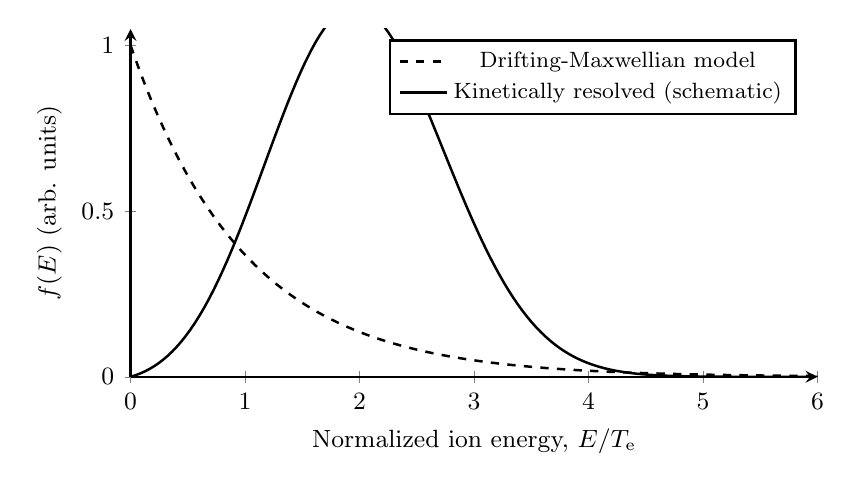
\begin{tikzpicture}
\begin{axis}[
 width=0.85\linewidth,
 height=6cm,
 xlabel={Normalized ion energy, $E/T_{\mathrm{e}}$},
 ylabel={$f(E)$ (arb. units)},
 xmin=0, xmax=6,
 ymin=0, ymax=1.05,
 axis lines=left,
 grid=none,
 legend pos=north east,
 ticklabel style={font=\small},
 label style={font=\small},
 legend style={font=\footnotesize, draw=black},
 line width=0.9pt,
]
\addplot[domain=0:6, samples=100, black, dashed] {exp(-x)};
\addlegendentry{Drifting-Maxwellian model}
\addplot[domain=0:6, samples=150, black, solid] {(x/1.6)*exp(-(x-1.6)^2/1.4)};
\addlegendentry{Kinetically resolved (schematic)}
\end{axis}
\end{tikzpicture}
\caption{Schematic comparison of two normalized ion energy distributions at the sheath edge: a single-exponential form implied by a drifting-Maxwellian analytic forward model (dashed), and a qualitatively broadened, peaked profile representative of a kinetically resolved collisionless-presheath calculation (solid). Both curves are illustrative analytic functions; neither represents measured or simulated data.}
\label{fig:iedf_schematic}
\end{figure}

\subsection{Noise injection, forward diagnostic models, and blind validation}

A dataset too clean --- free of the counting statistics, finite resolution, and systematic offsets present in any real instrument --- risks validating the inversion algorithm only in an unrealistically favourable regime. The synthetic traces are therefore processed through an explicit forward instrument model: Poisson counting noise set by an assumed integration time and detector sensitivity; a finite energy-resolution kernel (typically Gaussian, width set by grid transmission and analyser geometry) convolved with the ideal spectrum; and, where relevant, a slowly varying baseline representing secondary-electron background. Because the entire chain from PIC parameters through extraction, noise injection, and inversion is under the analyst's control, a strict \emph{blind} validation is possible, in which generating parameters are withheld from whoever runs the inversion until after the result is reported.

\section{Computational Cost and Reduced Models}

\subsection{Scaling of PIC cost with dimensionality and disparate scales}

The cost of an explicit electrostatic PIC simulation scales, at fixed domain size and duration, as the product of grid cells, superparticles per cell, and time steps. Each factor is set by a physical scale-separation ratio that is generically large in a real plasma--sheath system:
\begin{itemize}
\item cells spanning a domain of size $L$ while resolving $\lambda_{\mathrm{D}}$ scale as $(L/\lambda_{\mathrm{D}})^{d}$ in $d$ dimensions;
\item time steps needed to reach duration $\tau$ while resolving $\omega_{\mathrm{pe}}^{-1}$ (Eq.~\eqref{eq:wpe_dt}) scale as $\tau\,\omega_{\mathrm{pe}}$;
\item the mass ratio $m_{\mathrm{i}}/m_{\mathrm{e}}$ ($\sim 1.8\times10^{3}$ for hydrogen, up to $2\text{--}5\times10^{5}$ for heavy propellants) sets how many electron plasma periods must be resolved before the much slower ion transit, on which the sheath and presheath reach quasi-steady state, can be observed.
\end{itemize}
Because sheath-diagnostic applications span from a sub-millimetre sheath to a centimetre-to-metre bulk region, and ion transit time can exceed the electron plasma period by five or six orders of magnitude, a fully resolved, explicit electrostatic PIC simulation of an entire discharge is expensive even on HPC hardware, and a fully 3D, electromagnetic, multi-species run can require weeks of computation per operating point. This motivates the hierarchy of reduced and hybrid kinetic models below, each trading fidelity for cost, each validated against the fully kinetic ground truth of Section~\ref{sec:synthetic_ground_truth}.

\subsection{Hybrid and reduced-order kinetic models}

The most widely used cost-reduction strategy is the \emph{hybrid} approach: the computationally cheap species (usually electrons, whose small mass drives the restrictive $\omega_{\mathrm{pe}}\Delta t$ constraint) is treated with a fast fluid or Boltzmann-relation closure, while the species carrying the diagnostic information (usually ions) remains kinetic. Removing the electron plasma-period constraint lets the time step be set by the slower ion dynamics, typically a speed-up of two to three orders of magnitude. Hybrid fluid-electron/kinetic-ion schemes are the standard tool for large-scale Hall-thruster discharge modelling, where benchmarking against kinetic and experimental data shows where the hybrid closure remains valid and where it misses electron-kinetic effects such as anomalous cross-field transport \cite{ref0433}.

\subsection{Semi-kinetic trajectory simulation}

A further cost reduction, specific to the magnetized sheath and presheath problem, is \emph{kinetic trajectory simulation}: rather than a large ensemble of freely evolving superparticles subject to a mean field recomputed every step, a small number of representative ion trajectories are integrated through an iteratively determined potential profile, itself updated by enforcing quasi-neutrality using the trajectory-ensemble moments. Because the potential update, not an explicit field solve every step, is rate-limiting, this achieves substantial cost reduction while retaining the essential kinetic feature: an ion distribution built up self-consistently from particle histories rather than assumed \emph{a priori}. It has been developed for the 1D3V magnetized sheath, resolving the coupled presheath--Chodura-layer--Debye-sheath structure, and extended to multi-component sheaths tracking several ion species. Replacing the noisy explicit field solve with a smoother iterative construction yields low-noise distributions at a fraction of the cost, at the price of restricted geometry and a modeller-supplied coupling ansatz.

\subsection{Continuum kinetic (Vlasov) solvers as an alternative to particle noise}

A conceptually distinct route replaces the particle (Lagrangian, Monte-Carlo-sampled) representation of $f_{s}$ with a direct, grid-based (Eulerian) discretisation of the Vlasov equation, using finite-volume, spectral, or discontinuous-Galerkin methods on a phase-space mesh. Such solvers rely on no random sample and are entirely free of the statistical noise limiting the resolvable tail of $f_{\mathrm{i}}(v)$ in a standard PIC run, at the cost of a higher-dimensional grid and steeper memory/arithmetic scaling. Continuum kinetic and multi-fluid comparisons of classical sheath structure have quantified when a fluid closure remains adequate and when the noise-free continuum solution reveals structure a comparable-cost particle simulation would not resolve above its own statistical floor \cite{ref0659}. Reduced-basis and moment-closure techniques applied to the Vlasov system offer a further avenue for cost reduction. Because $\Gamma_{E}$ is a high-order moment disproportionately sensitive to the well-resolved tail, this monograph's ground-truth campaign favours high-$N_{\mathrm{ppc}}$ PIC runs, cross-checked where affordable against continuum benchmarks.

\section{Summary}

This chapter developed the kinetic foundation on which the synthetic ground-truth generation used elsewhere in this monograph rests. The Vlasov and Boltzmann equations were introduced as the exact phase-space description from which all fluid closures are derived by truncated moment-taking, and the circumstances under which that truncation fails at a plasma boundary --- collisionless presheath acceleration, trapped and reflected populations, non-stationary sheath edges --- were connected to the non-Maxwellian structure of $f_{\mathrm{i}}(v)$ that a kinetic Bohm criterion, rather than its fluid form, correctly captures. The particle-in-cell method was presented as the standard tool for solving Vlasov--Poisson in this regime, with attention to the weight--solve--gather--push cycle, the Boris integration scheme, and the coupled CFL, plasma-period, and Debye-length constraints that determine the grid, time step, and particle count a credible simulation must use. Monte Carlo collision and DSMC-coupled schemes extend this framework to collisional and multi-species regimes, and a survey of PIC studies of non-Maxwellian sheath structure, transient and RF-driven dynamics, and synthetic diagnostic extraction established the phenomena --- depleted low-velocity ion tails, RF-broadened bimodal distributions, multi-species flux partitioning --- that make a fully kinetic forward model indispensable for inversion validation. The chapter's central contribution is the forward--inverse validation loop of Section~\ref{sec:synthetic_ground_truth}, in which PIC-generated, noise-injected synthetic traces provide an independent ground truth for blind-testing later inversion algorithms. Finally, because PIC cost scales unfavourably with the disparate length and time scales of the plasma--sheath system, the chapter surveyed hybrid, semi-kinetic trajectory, and continuum alternatives that make routine, parameter-scanned kinetic sheath analysis practical, noting that the high-order moment defining $\Gamma_{E}$ places disproportionate demands on tail resolution that only a well-resolved kinetic calculation can reliably supply.

\chapter{Inverse Problems and Regularization}
\label{ch:inverse}

Every diagnostic statement made in the preceding chapters -- an ion energy distribution function reconstructed from a retarding-field analyzer sweep, an electron temperature inferred from a Langmuir-probe characteristic, a line-integrated emissivity converted into a local excited-state population -- is the output of an act of inference. A measured signal is never the physical quantity of interest; it is a transformation of that quantity, corrupted by noise, and the physicist's task is to undo the transformation. This chapter develops the theory of such inversions: what makes them different from ordinary problem solving, why naive inversion fails catastrophically, and what remedies exist, using as running examples the task organizing this monograph -- quantifying the ion energy flux $\Gamma_{E}$ delivered by a plasma sheath to a bounding surface, and reconstructing $f_{\mathrm{i}}(v)$, the sheath potential profile, or $(n_{\mathrm{e}}, T_{\mathrm{e}})$ from indirect, noisy, spectrally or temporally limited observations. Earlier chapters built forward models of the sheath; this chapter supplies the machinery to go the other way.

\section{Forward and Inverse Problems: The Forward Operator}
\label{sec:forward-inverse}

\subsection{Definitions and Terminology}

A \emph{forward problem} takes a fully specified physical model and predicts what an instrument coupled to the system would record. If $u$ denotes the unknown physical quantity -- a finite-dimensional parameter vector (e.g., $(n_{\mathrm{e}}, T_{\mathrm{e}}, T_{\mathrm{i}})$) or an infinite-dimensional function (e.g., $f_{\mathrm{i}}(v)$ or the sheath potential $\phi(x)$) -- and $g$ the corresponding noiseless data, the forward map is an operator $\mathcal{F}$ such that
\begin{equation}
g = \mathcal{F}[u].
\label{eq:forward-op}
\end{equation}
$\mathcal{F}$ encodes physics considered known and trustworthy: the kinetic theory of the sheath edge, the response function of a retarding-field energy analyzer (RFEA), the Abel geometry of a chord-integrating spectrometer, or the rate coefficients of a collisional-radiative model. The \emph{inverse problem} recovers $u$ given a measurement $g^{\delta}$ approximating $\mathcal{F}[u]$ to within a noise level $\delta$,
\begin{equation}
g^{\delta} = \mathcal{F}[u] + \eta, \qquad \|\eta\| \le \delta,
\label{eq:noisy-data}
\end{equation}
where $\eta$ folds measurement noise, digitization error, and unmodeled systematics into an effective stochastic term.

Three archetypal examples recur throughout this chapter.

\begin{enumerate}
\item \textbf{IEDF reconstruction from an RFEA sweep.} An RFEA collects a current $I(V)$ as a retarding grid voltage $V$ is swept. In the idealized planar, collisionless limit,
\begin{equation}
I(V) = A\, e \int_{v_{\min}(V)}^{\infty} v\, f_{\mathrm{i}}(v)\, \mathrm{d}v, \qquad v_{\min}(V) = \sqrt{2eV/m_{\mathrm{i}}},
\label{eq:rfea-forward}
\end{equation}
with $A$ the collector area and $m_{\mathrm{i}}$ the ion mass. $\mathcal{F}$ is a truncated moment transform, and the inverse recovers $f_{\mathrm{i}}(v)$ via differentiation, $f_{\mathrm{i}}(v) \propto - \mathrm{d}I/\mathrm{d}V$ at $eV = \tfrac{1}{2}m_{\mathrm{i}}v^{2}$ -- among the most notorious ill-posed operations in applied mathematics.
\item \textbf{Sheath potential profile from an IEDF.} Given a measured $f_{\mathrm{i}}(v)$ at the sheath edge, energy conservation along each ion trajectory, $\tfrac{1}{2}m_{\mathrm{i}}v^{2}(x) = \tfrac{1}{2}m_{\mathrm{i}}v_{0}^{2} + e[\phi(0)-\phi(x)]$, can be inverted for $\phi(x)$ once the launch-to-local velocity mapping is monotonic -- a nonlinear problem composing a kinetic transport model with the Poisson equation.
\item \textbf{Plasma density and temperature from line-integrated spectroscopy.} A chord-integrated emission signal relates to the local emissivity $\varepsilon(r)$, a nonlinear function of $n_{\mathrm{e}}(r)$ and $T_{\mathrm{e}}(r)$ through a collisional-radiative model, via a line integral, so recovering them requires inverting both the geometric integral and the nonlinear emissivity model.
\end{enumerate}

\subsection{Linear and Nonlinear Forward Operators}

When $\mathcal{F}$ is linear -- as in \cref{eq:rfea-forward} for fixed $v_{\min}(V)$, or a chord-integration (Radon/Abel) transform -- it discretizes to a matrix $K \in \mathbb{R}^{m \times n}$ acting on $u \in \mathbb{R}^{n}$:
\begin{equation}
g = Ku + \eta, \qquad K_{ij} = \int \psi_{i}(x)\, \kappa(x, x_{j})\, \mathrm{d}x,
\label{eq:linear-discrete}
\end{equation}
where $\kappa$ is the integral kernel of the forward map and $\psi_i$ are instrument response or basis functions. This is not an ordinary linear-algebra problem solvable by matrix inversion or unqualified least squares: $K$ from a physical integral kernel is almost always severely ill-conditioned.

When $\mathcal{F}$ is nonlinear, as in the emissivity-to-$(n_{\mathrm{e}},T_{\mathrm{e}})$ map, the machinery of this chapter applies either to a local linearization $\mathcal{F}[u_0 + \delta u] \approx \mathcal{F}[u_0] + J[u_0]\,\delta u$, with $J$ the Fréchet derivative, or within an iterative or Bayesian sampling scheme that repeatedly calls the forward model.

Inverse-problem theory developed for magnetohydrodynamic equilibrium diagnostics -- reconstructing current or pressure profiles from external magnetic measurements -- established many of the conceptual tools used here \cite{ref0687}.

\subsection{Discretization and the Rank-Deficiency Problem}

Physical forward operators of the kind in \cref{eq:linear-discrete} are typically \emph{smoothing}: the kernel $\kappa(x,x')$ averages $u$ over a neighborhood of $x$, so high-frequency structure is strongly attenuated in $g$. Wildly different unknowns $u$ can thus map to data differing by less than the noise floor $\delta$ -- the root cause of everything that follows, examined through the SVD in \cref{sec:regularization}.

\section{Ill-Posedness in the Sense of Hadamard}
\label{sec:hadamard}

\subsection{The Three Conditions}

Hadamard's classical definition, formulated for boundary value problems in partial differential equations, states that a problem is \emph{well-posed} iff it satisfies three conditions simultaneously:

\begin{table}[htbp]
\centering
\caption{Hadamard's conditions for well-posedness, and their typical failure mode for IEDF reconstruction from an RFEA sweep.}
\label{tab:hadamard}
\begin{tabularx}{\textwidth}{@{}l >{\raggedright\arraybackslash}X >{\raggedright\arraybackslash}X@{}}
\toprule
Condition & Statement & Typical failure in plasma inverse problems \\
\midrule
Existence & For every admissible $g$ there exists at least one $u$ with $\mathcal{F}[u] = g$. & Noise $\eta$ almost never lies in the range of $\mathcal{F}$; an exact solution to $\mathcal{F}[u]=g^{\delta}$ generally does not exist. \\
Uniqueness & The solution $u$, if it exists, is unique. & The null space of $K$ (or its numerical near-null-space) is nontrivial; several distinct $u$ produce data differing by less than $\delta$. \\
Stability & $u$ depends continuously on $g$: small perturbations in $g$ produce small perturbations in $u$. & Smoothing kernels have singular values decaying toward zero; the (pseudo)inverse amplifies noise without bound as truncation is relaxed. \\
\bottomrule
\end{tabularx}
\end{table}

A problem violating any one condition is \emph{ill-posed}. The RFEA differentiation problem violates stability outright: differentiation is unbounded on the space of noisy functions, so arbitrarily small noise in $I(V)$ produces an arbitrarily large error in the naively differentiated $f_{\mathrm{i}}(v)$. Abel inversion is similarly unstable near the geometric axis, where the inversion kernel develops an integrable but numerically troublesome singularity. Sturm--Liouville inverse spectral problems -- recovering an unknown potential from spectral data, structurally analogous to a sheath potential profile from a measured energy spectrum -- hold existence and uniqueness only under restrictive regularity assumptions; a discontinuous or cusped sheath-edge potential, as in idealized Bohm-criterion matching, is precisely the class for which uniqueness theorems require the most care.

\subsection{Existence}

Non-existence of an exact solution is, in practice, the least dangerous failure, resolved by relaxing "solution" from an exact preimage to a best approximation in a chosen norm,
\begin{equation}
\hat{u} = \arg\min_{u} \| \mathcal{F}[u] - g^{\delta} \|^{2},
\label{eq:least-squares}
\end{equation}
i.e., a least-squares (generalized-solution) formulation. This alone does not restore well-posedness: \cref{eq:least-squares} may still lack a minimizer, have several, or depend discontinuously on $g^{\delta}$.

\subsection{Uniqueness}

Uniqueness fails whenever the forward operator has a nontrivial null space, $\mathcal{N}(K) = \{v : Kv = 0\}$: any solution $u$ can be modified by an element of $\mathcal{N}(K)$ without changing the predicted data. This is diagnosed from the SVD of $K$,
\begin{equation}
K = U \Sigma V^{\mathrm{T}} = \sum_{i=1}^{r} \sigma_{i}\, u_{i} v_{i}^{\mathrm{T}}, \qquad \sigma_{1} \ge \sigma_{2} \ge \cdots \ge \sigma_{r} > 0,
\label{eq:svd}
\end{equation}
where $r = \mathrm{rank}(K)$. Any $v_i$ with $i > r$ spans the exact null space; more troublingly, singular values of a smoothing kernel decay toward zero without a clean spectral gap, so the \emph{numerical} null space -- singular vectors below the noise floor -- is large, its boundary a matter of judgment rather than sharp rank. Stability-estimate analyses of inverse-scattering and inverse-source problems formalize this graded loss of uniqueness: attainable resolution degrades continuously with the assumed smoothness of the unknown, directly relevant to the RFEA differentiation problem.

\subsection{Stability}

Stability is most consequential for plasma diagnostics, since it governs how measurement noise propagates into the reconstruction. For the linear operator of \cref{eq:svd}, the naive (Moore--Penrose) generalized inverse is
\begin{equation}
u^{\dagger} = K^{\dagger} g^{\delta} = \sum_{i=1}^{r} \frac{u_{i}^{\mathrm{T}} g^{\delta}}{\sigma_{i}}\, v_{i}.
\label{eq:pseudoinverse}
\end{equation}
Decomposing $g^{\delta} = Ku_{\mathrm{true}} + \eta$ and substituting,
\begin{equation}
u^{\dagger} = u_{\mathrm{true}} + \sum_{i=1}^{r} \frac{u_{i}^{\mathrm{T}} \eta}{\sigma_{i}}\, v_{i},
\label{eq:noise-amplification}
\end{equation}
so every noise component along $u_i$ is amplified by $1/\sigma_i$. Smoothing operators produce singular values that decay geometrically or faster, so the smallest-$\sigma_i$ terms dominate and $u^{\dagger}$ is overwhelmed by amplified noise however small $\delta$ is -- why naive differentiation of a noisy RFEA characteristic, or naive inversion of a chord-integration matrix, produces wildly oscillating reconstructions bearing no resemblance to the true $f_{\mathrm{i}}(v)$ or $n_{\mathrm{e}}(r)$. Regularization suppresses the small-$\sigma_i$ terms at an acceptable cost in resolution and bias.

Model problems for diffusion and wave equations offer tractable settings where this instability, and its cure, can be stated exactly. Backward-in-time diffusion problems are exponentially ill-posed in the sense of \cref{eq:noise-amplification}, with $1/\sigma_i$ growing exponentially in mode index; regularization for such problems, and for the analogous inverse heat-conduction problem, formalizes the stability-versus-resolution trade-off for a smoothing operator closely analogous to the RFEA and Abel-transform kernels here. Even hyperbolic (finite-speed) inverse wave problems can harbor mild ill-posedness once discretization and finite bandwidth are accounted for, so ill-posedness is a property of the operator-and-data pair, not merely of smoothing kernels. Inverse conductivity problems with discontinuous conductivities -- close to a sheath potential profile with a sharp presheath-sheath transition -- show that discontinuities do not by themselves destroy well-posedness, provided the regularization functional respects rather than penalizes sharp transitions.

\section{Regularization}
\label{sec:regularization}

Regularization trades exact (or least-squares) fidelity to the data for a controlled, stable dependence of the reconstruction on the data. All regularization methods share the same structure: an auxiliary functional $\mathcal{R}[u]$, encoding a prior belief about the smoothness, sparsity, or shape of the true solution, is combined with the data-misfit functional, with a scalar parameter $\alpha > 0$ balancing the two.

\subsection{Tikhonov Regularization}

The most widely used scheme replaces \cref{eq:least-squares} with the penalized least-squares problem
\begin{equation}
u_{\alpha} = \arg\min_{u} \left\{ \| Ku - g^{\delta} \|_{2}^{2} + \alpha^{2} \| Lu \|_{2}^{2} \right\},
\label{ch14-eq:tikhonov}
\end{equation}
where $L$ is a regularization operator -- the identity for zeroth-order Tikhonov, a first derivative to penalize roughness, or a second derivative to penalize curvature. The minimizer follows from the normal equations,
\begin{equation}
\left( K^{\mathrm{T}} K + \alpha^{2} L^{\mathrm{T}} L \right) u_{\alpha} = K^{\mathrm{T}} g^{\delta},
\label{eq:tikhonov-normal}
\end{equation}
which, unlike $K^{\mathrm{T}} K u = K^{\mathrm{T}} g^{\delta}$, remain well-conditioned because $\alpha^{2} L^{\mathrm{T}} L$ lifts the smallest eigenvalues of $K^{\mathrm{T}}K$ away from zero. In the singular-value basis for $L = I$,
\begin{equation}
u_{\alpha} = \sum_{i=1}^{r} \frac{\sigma_{i}^{2}}{\sigma_{i}^{2} + \alpha^{2}} \cdot \frac{u_{i}^{\mathrm{T}} g^{\delta}}{\sigma_{i}}\, v_{i},
\label{eq:tikhonov-svd}
\end{equation}
identical to \cref{eq:pseudoinverse} multiplied by \emph{filter factors} $f_{i}(\alpha) = \sigma_{i}^{2}/(\sigma_{i}^{2}+\alpha^{2})$: for $\sigma_{i} \gg \alpha$, $f_{i} \to 1$; for $\sigma_{i} \ll \alpha$, $f_{i} \to 0$ and the noise-dominated component is smoothly suppressed -- a soft, continuously tunable low-pass filter in the singular-value domain, not a generic smoothing in physical space.

Tomographic laser absorption spectroscopy of combustion and plasma media is a direct precedent for applying \cref{ch14-eq:tikhonov} to a chord-integration operator structurally identical to sheath-adjacent emission diagnostics, demonstrating the fidelity gained once the naive pseudoinverse is replaced by \cref{eq:tikhonov-svd} \cite{ref0677}. Refinements tailored to EXAFS spectroscopy address how $\alpha$ should be chosen -- the subject of \cref{sec:l-curve} \cite{ref0695}. More generally, $\mathcal{R}[u]$ need not act directly on $u$ but can penalize the mismatch between two auxiliary reconstructions under complementary conditions, as when an RFEA-derived and a Langmuir-probe-derived estimate of the same parameter are combined.

\subsection{Truncated Singular Value Decomposition}

An alternative, simpler scheme truncates \cref{eq:pseudoinverse} at a cutoff index $k$ rather than smoothly damping it:
\begin{equation}
u_{k} = \sum_{i=1}^{k} \frac{u_{i}^{\mathrm{T}} g^{\delta}}{\sigma_{i}}\, v_{i}, \qquad k < r.
\label{eq:tsvd}
\end{equation}
Truncated SVD (TSVD) is a hard filter, $f_i = 1$ for $i \le k$, $0$ otherwise, with $k$ playing the role of $\alpha$. TSVD and Tikhonov regularization are asymptotically equivalent for well-chosen $k$ and $\alpha$, both belonging to the family of \emph{spectral filtering} methods; the choice is largely numerical convenience, since Tikhonov via \cref{eq:tikhonov-normal} scales better to large, sparse, or matrix-free operators. Iterative solvers (Landweber, conjugate-gradient least squares) achieve the same effect implicitly, with iteration count as the regularization parameter and early stopping equivalent to a spectral filter. Wavelet-domain representations generalize further, expanding $u$ sparsely in a basis of localized features and thresholding coefficients -- relevant to the sharp gradients of the sheath and presheath.

\subsection{Total Variation Regularization}

Tikhonov regularization and TSVD both penalize the norm of $u$ or its derivatives so that, under strong regularization, sharp features are smoothed out -- a serious liability for sheath reconstruction, where the sheath edge has rapidly changing charge density and an IEDF at a biased surface can have a sharp cutoff at the maximum ion energy set by the sheath potential drop. Total variation (TV) regularization replaces the quadratic penalty with the total variation seminorm,
\begin{equation}
u_{\alpha}^{\mathrm{TV}} = \arg\min_{u} \left\{ \| Ku - g^{\delta} \|_{2}^{2} + \alpha \, \mathrm{TV}(u) \right\}, \qquad \mathrm{TV}(u) = \int \left| \frac{\mathrm{d}u}{\mathrm{d}x} \right| \mathrm{d}x,
\label{eq:tv}
\end{equation}
an $L^1$-type penalty that does not force the derivative small everywhere but penalizes total variation regardless of distribution. TV-regularized reconstructions can thus contain sharp jumps at essentially no penalty, provided variation elsewhere stays small -- unlike Tikhonov reconstructions, which spread sharp features over a width set by $\alpha$. Convergence theory establishes conditions under which $u_{\alpha}^{\mathrm{TV}}$ converges to the true solution as $\alpha, \delta \to 0$ in a coordinated way, clarifying why TV regularization, despite lacking the closed-form solution of \cref{eq:tikhonov-svd}, remains well-posed and provably convergent \cite{ref0692}.

\begin{table}[htbp]
\centering
\caption{Qualitative comparison of the three regularization families, as applied to a smoothing forward operator of the type in \cref{eq:linear-discrete}. Properties are schematic, intended to orient method selection rather than substitute for a problem-specific study.}
\label{tab:regularization-comparison}
\begin{tabularx}{\textwidth}{@{}l >{\raggedright\arraybackslash}X >{\raggedright\arraybackslash}X >{\raggedright\arraybackslash}X@{}}
\toprule
Property & Tikhonov & TSVD & Total variation \\
\midrule
Penalty type & quadratic ($L^2$) & hard spectral cutoff & $L^1$ of derivative \\
Closed-form solution & yes (linear system) & yes (SVD truncation) & no (nonlinear optimization) \\
Edge/discontinuity handling & smooths across edges & smooths across edges & preserves sharp edges \\
Parameter to choose & $\alpha$ (continuous) & $k$ (discrete) & $\alpha$ (continuous) \\
Typical use in this monograph & smooth $n_{\mathrm{e}}(r)$, $T_{\mathrm{e}}(r)$ profiles & rapid SVD-based screening & sheath-edge cutoff in $f_{\mathrm{i}}(v)$ \\
\bottomrule
\end{tabularx}
\end{table}

\subsection{The L-Curve and Regularization-Parameter Choice}
\label{sec:l-curve}

No regularization scheme is complete without a rule for choosing $\alpha$ (or $k$): too small reintroduces the noise amplification of \cref{eq:noise-amplification}, too large biases the reconstruction toward excessive smoothness. Two families of rule are in common use.

\emph{A priori and discrepancy-based rules} require an estimate of $\delta$, choosing $\alpha$ so the residual matches the expected noise, $\|Ku_{\alpha} - g^{\delta}\| \approx \delta$ (Morozov's discrepancy principle), or use generalized cross-validation (GCV), minimizing a leave-one-out prediction error without an explicit $\delta$.

\emph{The L-curve method} is an a posteriori, data-driven heuristic requiring no estimate of $\delta$. It plots, on log-log axes and parametrically in $\alpha$, the residual norm against the solution seminorm,
\begin{equation}
\text{L-curve:} \quad \Big( \log \| K u_{\alpha} - g^{\delta} \|_{2},\ \log \| L u_{\alpha} \|_{2} \Big), \qquad \alpha \in (0, \infty).
\label{eq:l-curve-def}
\end{equation}
For small $\alpha$ the residual is small but the seminorm large; for large $\alpha$ the reverse holds. The curve typically has a pronounced corner separating a near-vertical, residual-dominated branch from a near-horizontal, regularization-dominated branch, and the point of maximum curvature is taken as $\alpha^{\ast}$. \Cref{ch14-fig:lcurve} shows a schematic L-curve, generated from an analytic filter-factor model rather than measured data, illustrating the geometric criterion.

\begin{figure}[htbp]
\centering
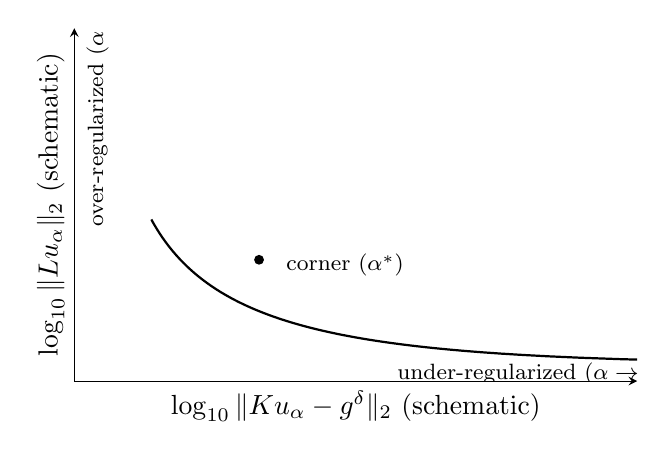
\begin{tikzpicture}
\begin{axis}[
 width=0.72\textwidth,
 height=0.5\textwidth,
 xlabel={$\log_{10}\|Ku_{\alpha}-g^{\delta}\|_2$ (schematic)},
 ylabel={$\log_{10}\|Lu_{\alpha}\|_2$ (schematic)},
 domain=0.05:6,
 samples=200,
 axis lines=left,
 every axis plot/.append style={thick, black},
 ticks=none,
 xmin=0, xmax=3.2,
 ymin=0, ymax=3.2,
]
\addplot[black, thick] ({0.15+ln(1+2/x)}, {0.15+ln(1+x/2.2)});
\node[draw, circle, fill=black, inner sep=1.1pt] at (axis cs:1.05,1.10) {};
\node[anchor=west] at (axis cs:1.15,1.05) {\footnotesize corner ($\alpha^{\ast}$)};
\node[anchor=north] at (axis cs:2.6,0.25) {\footnotesize under-regularized ($\alpha\to0$)};
\node[anchor=south, rotate=90] at (axis cs:0.25,2.6) {\footnotesize over-regularized ($\alpha\to\infty$)};
\end{axis}
\end{tikzpicture}
\caption{Schematic, illustrative L-curve generated from an explicit analytic filter-factor model (not measured or simulated diagnostic data), showing the corner separating the noise-amplification branch (small $\alpha$) from the over-smoothing branch (large $\alpha$). The point of maximum curvature, marked, is the L-curve estimate of $\alpha^{\ast}$.}
\label{ch14-fig:lcurve}
\end{figure}

Optimal-parameter-selection studies for Tikhonov-regularized EXAFS inversion benchmark the L-curve criterion against the discrepancy principle and GCV for an operator of comparable conditioning to the RFEA and Abel-inversion kernels here, finding the L-curve corner robust when the noise level is only approximately known -- the typical situation for laboratory sheath diagnostics \cite{ref0695}.

\section{Bayesian Formulation}
\label{sec:bayesian}

\subsection{Likelihood, Prior, and Posterior}

The deterministic regularization framework of \cref{sec:regularization} has an exact probabilistic counterpart that both justifies and generalizes it. The unknown $u$ is a random variable with a prior density $p(u)$ encoding everything believed, before any data are examined, about plausible sheath potentials, IEDFs, or density profiles -- smoothness, positivity, or bounds such as $f_{\mathrm{i}}(v) \ge 0$. The noisy data relate to $u$ through a likelihood $p(g^{\delta}\,|\,u)$ built from $\mathcal{F}$ and a noise model; for additive Gaussian noise with covariance $C_{\eta}$,
\begin{equation}
p(g^{\delta}\,|\,u) \propto \exp\!\left[ -\tfrac{1}{2} \left( g^{\delta} - \mathcal{F}[u] \right)^{\mathrm{T}} C_{\eta}^{-1} \left( g^{\delta} - \mathcal{F}[u] \right) \right].
\label{ch14-eq:likelihood}
\end{equation}
Bayes' theorem combines prior and likelihood into the posterior density,
\begin{equation}
p(u\,|\,g^{\delta}) = \frac{ p(g^{\delta}\,|\,u)\, p(u) }{ \int p(g^{\delta}\,|\,u')\, p(u')\, \mathrm{d}u' },
\label{eq:bayes}
\end{equation}
representing the complete state of knowledge about $u$ after the measurement. All subsequent inferences -- point estimates, error bars, and derived quantities such as $\Gamma_{E} = \int \tfrac{1}{2} m_{\mathrm{i}} v^{2} \cdot v f_{\mathrm{i}}(v)\, \mathrm{d}v$ -- are obtained by summarizing this posterior.

\subsection{Maximum A Posteriori Estimation and its Equivalence to Tikhonov Regularization}

The MAP estimator maximizes \cref{eq:bayes}, equivalently minimizing its negative logarithm. For a Gaussian prior $p(u) \propto \exp[-\tfrac{1}{2}(u-u_0)^{\mathrm{T}} C_{u}^{-1} (u-u_0)]$ with covariance $C_u$ and the Gaussian likelihood linearized as $\mathcal{F}[u] \approx Ku$,
\begin{equation}
u_{\mathrm{MAP}} = \arg\min_{u} \left\{ \left( g^{\delta} - Ku \right)^{\mathrm{T}} C_{\eta}^{-1} \left( g^{\delta} - Ku \right) + u^{\mathrm{T}} C_{u}^{-1} u \right\},
\label{eq:map}
\end{equation}
which, writing $C_{\eta} = \sigma_{\eta}^{2} I$ and $C_{u}^{-1} = (\alpha^2/\sigma_\eta^2) L^{\mathrm{T}}L$, is algebraically identical to \cref{ch14-eq:tikhonov}. This is a structural fact, not a coincidence: Tikhonov regularization \emph{is} Gaussian MAP estimation, and the choice of $L$ \emph{is} the choice of prior covariance $C_u$. TV regularization corresponds to a non-Gaussian (Laplace-type, heavy-tailed) prior on $u$'s derivative, which is why it tolerates occasional large jumps at a much lower probabilistic "cost" than a Gaussian prior would.

\subsection{Posterior Uncertainty and Credible Intervals}

Beyond the point estimate $u_{\mathrm{MAP}}$, the linear-Gaussian case yields the posterior covariance in closed form,
\begin{equation}
C_{\mathrm{post}} = \left( K^{\mathrm{T}} C_{\eta}^{-1} K + C_{u}^{-1} \right)^{-1},
\label{ch14-eq:posterior-cov}
\end{equation}
whose diagonal gives pointwise posterior variances -- and hence credible intervals -- for every component of $u$, including $\Gamma_{E}$ once propagated through the nonlinear moment integral, a substantive advantage over \cref{sec:regularization}, which supplies a single reconstruction $u_{\alpha}$ but no principled measure of confidence. The off-diagonal structure of $C_{\mathrm{post}}$ additionally reveals \emph{correlations} between reconstructed values at nearby velocities or radii, essential for propagating uncertainty into any derived quantity, since naively summing independent pointwise variances underestimates the true uncertainty.

Gaussian-process priors generalize the Gaussian $C_u$ above by specifying the prior covariance directly as a smooth kernel over the domain of $u$, rather than through a differential operator $L$. Bayesian modelling of Thomson-scattering and interferometer data with such priors demonstrates this in a magnetically confined plasma, jointly inferring density and temperature profiles with calibrated uncertainty bands and propagating them into derived quantities, directly analogous to propagating IEDF uncertainty into $\Gamma_{E}$ \cite{ref0683}. Bayesian inference from collective Thomson scattering on a transient gas-puff pinch extends the methodology to a rapidly evolving plasma, updating the posterior self-consistently as channels with different forward operators are combined \cite{ref0684}. A multi-instrument analysis system for divertor plasma characteristics fuses diagnostics -- each with its own $\mathcal{F}_j$ and likelihood $p_j(g_j^{\delta}\,|\,u)$ -- into a joint posterior $p(u\,|\,\{g_j^{\delta}\}) \propto p(u) \prod_j p_j(g_j^{\delta}\,|\,u)$, relevant whenever an energy flux estimate is cross-validated using RFEA, Langmuir-probe, and spectroscopic data \cite{ref0685}.

\subsection{Computational Considerations}

For nonlinear forward operators -- joint chord-integrated/collisional-radiative inversion, or nonlinear sheath-potential reconstruction -- the posterior of \cref{eq:bayes} is generally not Gaussian and \cref{ch14-eq:posterior-cov} does not apply exactly. It is then characterized either by local linearization about the MAP point (a Laplace approximation, \cref{ch14-eq:posterior-cov} with $K \to J[u_{\mathrm{MAP}}]$) or by direct Markov-chain Monte Carlo sampling, the price of a faithful characterization whenever nonlinearity or a non-Gaussian prior makes the Gaussian approximation inadequate.

\section{Plasma Tomography and Spectroscopic Inversion as Precedents}
\label{sec:tomography}

The ion-energy-flux inverse problems motivating this chapter belong to a larger family: recovering a spatially or spectrally resolved plasma quantity from indirect measurements. This section surveys that family for forward-operator structure, conditioning, and regularization strategies that transfer directly to sheath diagnostics.

\subsection{Geometric (Tomographic) Inversion}

Plasma tomography reconstructs a two- or three-dimensional emissivity, density, or temperature field from line-integrated (chord) measurements collected by cameras, bolometer arrays, or interferometers viewing the plasma from several directions. The forward operator is the Radon transform, or the Abel transform for axisymmetric sources viewed along one direction,
\begin{equation}
g(p, \theta) = \int_{-\infty}^{\infty} u(p\cos\theta - s\sin\theta,\ p\sin\theta + s\cos\theta)\, \mathrm{d}s,
\label{eq:radon}
\end{equation}
discretized into a sparse matrix $K$ whose rows are chords and columns are pixels or annular shells. The sparsity and limited-angle coverage of realistic chord geometries -- far fewer viewing directions than in medical or industrial tomography -- exacerbate the rank deficiency of \cref{sec:hadamard}, addressed by dedicated optical-tomography inversion algorithms that established the discretization, regularization, and error-propagation framework used throughout this literature. The Abel transform retains an analytic inversion formula in the noise-free limit, but a weak singularity near the symmetry axis makes the noisy inversion numerically delicate; treatments of Abel inversion for laser-induced plasma imaging address noise and incomplete data within a framework analogous to \cref{ch14-eq:tikhonov}.

\subsection{Spectroscopic Inversion}

A second precedent class arises when the forward operator involves a physically nonlinear spectroscopic model, typically a collisional-radiative model relating emissivity to $n_{\mathrm{e}}$ and $T_{\mathrm{e}}$. Radially resolved optical emission spectral imaging of atmospheric-pressure plasmas illustrates the combined geometric-and-spectroscopic problem, where the chord geometry and atomic model must be inverted jointly, not sequentially, to avoid propagating a geometric artifact into the spectroscopic interpretation -- relevant to sheath-adjacent OES or LIF signals unfolded both along the line of sight and through a nonlinear intensity-to-$f_{\mathrm{i}}(v)$ or $(n_{\mathrm{e}}, T_{\mathrm{e}})$ relationship.

A further relevant problem is recovering the electron energy distribution function from an indirect spectral signature. Regularized inversion of Bremsstrahlung emission spectra from pulse-height data shows that count-based (Poisson) noise models -- appropriate whenever data are photon or particle counts, as for energetic-particle diagnostics near a sheath -- require a modified likelihood and regularization functional matching low-count-rate statistics rather than the Gaussian Tikhonov framework.

\subsection{Transfer to Sheath and Ion-Energy-Flux Diagnostics}

The unifying lesson is that the pathology afflicting sheath-adjacent inverse problems -- RFEA differentiation, Abel-type inversion of chord-integrated OES or LIF signals, joint geometric-spectroscopic unfolding of $(n_{\mathrm{e}}, T_{\mathrm{e}})$ feeding into $u_{\mathrm{B}}$ and hence $\Gamma_{E}$ -- is not a peculiarity of sheath physics but an instance of a well-characterized problem class. Every tool surveyed in \cref{sec:regularization,sec:bayesian} transfers with no change in mathematical structure, only in the form of $\kappa(x,x')$ and the choice of $L$ or $C_u$.

\section{Conditioning, Resolution, and Error Propagation}
\label{sec:conditioning}

\subsection{Condition Number}

The numerical severity of an inverse problem's ill-posedness is summarized by
\begin{equation}
\kappa(K) = \frac{\sigma_{\max}}{\sigma_{\min}},
\label{eq:condition-number}
\end{equation}
with $\sigma_{\max}, \sigma_{\min}$ the largest and smallest nonzero singular values of $K$. A large $\kappa(K)$ signals a poorly constrained solution space; for RFEA, Abel, and collisional-radiative kernels, $\kappa(K)$ at any practical discretization is typically many orders of magnitude, confirming \cref{sec:hadamard}. Regularization replaces $K$ by $K_{\alpha}^{\dagger}$, whose effective condition number on the recovered subspace is finite.

\subsection{Resolution and the Averaging Kernel}

A regularized reconstruction does not recover the true $u$ exactly even without noise, since the filter factors of \cref{eq:tikhonov-svd} (or the truncation of \cref{eq:tsvd}) suppress high-index components regardless of whether they carry noise or signal. This systematic distortion is characterized by the \emph{resolution} or \emph{averaging-kernel} matrix,
\begin{equation}
R_{\alpha} = K_{\alpha}^{\dagger} K, \qquad u_{\alpha} = R_{\alpha}\, u_{\mathrm{true}} + \left(\text{noise term}\right),
\label{eq:resolution-matrix}
\end{equation}
which reduces to the identity in the unregularized limit and otherwise smears $u_{\mathrm{true}}$: the $i$-th row of $R_\alpha$ describes which combination, and over what width, of $u_{\mathrm{true}}$ contributes to $u_{\alpha,i}$. Its full width at half maximum is the rigorous definition of resolution -- sharper means finer resolution but, through \cref{eq:tikhonov-svd}, smaller $\alpha$ and larger noise amplification via \cref{eq:noise-amplification}. No choice of $\alpha$ escapes this trade-off; every reported reconstruction in this monograph implicitly states a chosen point on this curve, not the "true," fully resolved quantity.

\subsection{Error Propagation into Derived Quantities}

The physical target of this monograph is a nonlinear functional of the reconstructed IEDF,
\begin{equation}
\Gamma_{E} = \int_{0}^{\infty} \tfrac{1}{2} m_{\mathrm{i}} v^{2} \cdot v\, f_{\mathrm{i}}(v)\, \mathrm{d}v,
\label{eq:energy-flux-functional}
\end{equation}
so the uncertainty in $\Gamma_{E}$ must be obtained by propagating the full posterior (or regularized) covariance of $f_{\mathrm{i}}(v)$ through this integral, not by averaging pointwise uncertainties. To first order, with sensitivity kernel $w(v) = \tfrac{1}{2}m_{\mathrm{i}}v^{3}$,
\begin{equation}
\mathrm{Var}[\Gamma_{E}] \approx \iint w(v)\, C_{\mathrm{post}}(v,v')\, w(v')\, \mathrm{d}v\, \mathrm{d}v',
\label{ch14-eq:error-propagation}
\end{equation}
depending on the full off-diagonal structure of $C_{\mathrm{post}}(v,v')$. Because $w(v) \propto v^3$ emphasizes the high-velocity tail of $f_{\mathrm{i}}(v)$ -- precisely where the RFEA differentiation problem is least well resolved, since high energies sample the sparse extreme of the sweep -- the propagated uncertainty on $\Gamma_{E}$ is dominated by the poorly resolved tail, not the well-resolved bulk. Reporting a point estimate without correctly propagated, correlation-aware uncertainty is a common and consequential error.

\subsection{Diagnosing Resolution Loss in Practice}

$R_{\alpha}$ and $C_{\mathrm{post}}$ are both computable at $\alpha^{\ast}$ directly from the SVD or Cholesky factorization already required for the reconstruction, so reporting resolution and correlated uncertainty costs little extra. The L-curve corner, filter factors, resolution matrix, and propagated uncertainty together form a diagnostic package that should accompany any reconstructed sheath quantity: a point estimate alone is not scientifically complete given \cref{sec:hadamard}.

\section{Summary}

This chapter treats the recovery of sheath and plasma quantities from indirect diagnostic data as a genuine inverse problem. The forward operator $\mathcal{F}$ -- whether the transform relating an RFEA sweep to $f_{\mathrm{i}}(v)$, a chord-integrating geometric integral, or the nonlinear map of a collisional-radiative model -- is generically smoothing, and its inversion is ill-posed in the sense of Hadamard: existence is restored by a least-squares formulation, while uniqueness and stability remain compromised by a near-null space and singular-value decay that amplifies noise without bound in the naive pseudoinverse. Regularization -- Tikhonov, truncated SVD, and total variation -- restores a controlled, stable dependence on the data by penalizing noise-dominated components, at an unavoidable cost in resolution captured by the averaging-kernel matrix; the trade-off is set by the L-curve criterion or related discrepancy-based and cross-validation rules. The Bayesian formulation subsumes this picture, identifying MAP estimation under a Gaussian prior with Tikhonov regularization while furnishing a full posterior from which credible intervals and correlations follow directly, and extending to non-Gaussian priors, nonlinear operators, and multi-diagnostic fusion. Plasma tomography and spectroscopic inversion provide validated precedents that transfer directly to sheath and ion-energy-flux diagnostics: the same pathologies, remedies, and resolution-versus-noise trade-off govern both. Its central conclusion is that any reconstructed sheath quantity -- an IEDF, a potential profile, a density or temperature profile, or $\Gamma_{E}$ itself -- is scientifically incomplete without a correctly propagated statement of its resolution and correlated uncertainty, tools that are a low-cost byproduct of the regularized or Bayesian inversion procedure by which the quantity was obtained.

\chapter{A Physics-Constrained Inversion Framework for Ion Energy Flux}
\label{ch:pci}

The preceding chapters established the kinetic and fluid description of the plasma sheath, the forward physics of four optical diagnostics (OES, LIF, Thomson scattering, and interferometry), the machinery of ill-posed inverse problems, and the philosophy of diagnostic fusion. This chapter assembles these into the Physics-Constrained Inversion (PCI) framework: an estimation architecture built on the claim that the ion energy flux $\GammaE$ delivered to a plasma-facing surface, unobservable by any single non-intrusive instrument, is over-determined by the \emph{combination} of four instruments once required to remain consistent with sheath kinetic theory. Reconstructing $\GammaE$ then ceases to be four independent, rank-deficient inversions stitched together and becomes one jointly well-posed nonlinear estimation problem, in which sheath physics supplies the regularization that noisy, incomplete optical data cannot supply alone. The chapter states the problem formally, derives the forward operators, develops the physics constraints as regularizers, solves the regularized objective, extends it to transient and RF-periodic dynamics, describes the numerical pipeline, and closes with the assumptions underlying the construction and their validation.

\section{Formal Statement of the Reconstruction Problem}
\label{sec:pci-formal}

\subsection{Philosophy: estimation rather than sequential deconvolution}

A conventional workflow treats each instrument as a self-contained deconvolution: a Boltzmann plot reduces OES line ratios to $(\ne,\Te)$; an LIF line shape is fitted to a drifting Maxwellian for $\Ti$; a TS spectrum is fitted independently for a second, often inconsistent, $(\ne,\Te)$; an interferometric phase shift is Abel-inverted for $\ne$. Each analysis is individually ill-posed whenever the true distribution departs from the assumed parametric family, and discards covariance information that could correct an earlier estimate. PCI instead poses a single estimation problem over a shared state $\mathbf{m}$ from which all four channels, and $\GammaE$, are computed by explicit, jointly consistent forward operators \cite{ref0711,ref0727} -- the move underlying integrated data analysis (IDA) in magnetic confinement fusion \cite{ref0707,ref0712}, specialized here to the sheath boundary layer, where the regularizing physics is the kinetic and fluid closure of the plasma--sheath transition itself.

\subsection{The unknown state vector}

Let $\mathbf{m}\in\mathbb{R}^{p}$ denote the unknown state of the bulk plasma, presheath, and sheath at a given location and, in the steady formulation of this section, a single instant, partitioned into four blocks:
\begin{align}
\mathbf{m} &= \big(\, \underbrace{\ne,\ \Te,\ \Ti,\ \kappa_{\mathrm e}}_{\text{bulk/presheath moments}}\ ,\ \underbrace{c_{1},\dots,c_{K}}_{\text{IVDF basis coefficients}}\ ,\notag\\
&\qquad \underbrace{V_{0},\ s,\ \gamma_{\mathrm{se}},\ \mathrm{Kn}_{\mathrm i}}_{\text{sheath structure}}\ ,\ \underbrace{\{V_{n},\psi_{n}\}_{n=1}^{N}}_{\text{RF harmonic content (time-resolved case)}} \,\big) \, . \label{eq:state}
\end{align}
$\kappa_{\mathrm e}$ is a shape parameter admitting a controlled departure of the bulk electron energy distribution function (EEDF) from Maxwellian, consistent with the sensitivity of the sheath-formation criterion to non-Maxwellian electrons \cite{ref0090}. The coefficients $c_{1},\dots,c_{K}$ parametrize the ion velocity distribution function (IVDF) $f_{\mathrm i}(v)$ at the sheath edge in a truncated basis (Hermite functions, B-splines, mixture-of-Gaussians):
\begin{equation}
f_{\mathrm i}(v) \;=\; \sum_{k=1}^{K} c_{k}\, \psi_{k}(v)\, , \qquad \int_{-\infty}^{\infty} f_{\mathrm i}(v)\,\mathrm dv = \ni \, . \label{eq:ivdf-basis}
\end{equation}
$V_{0}$ is the time-averaged sheath potential drop, $s$ the sheath thickness, $\gamma_{\mathrm{se}}$ the secondary-electron emission yield, and $\mathrm{Kn}_{\mathrm i}=\lambda_{\mathrm{in}}/s$ the ion Knudsen number controlling the collisionless-to-collisional crossover \cite{ref0077}. The final block, populated only in the time-resolved formulation of \cref{sec:pci-time}, carries the amplitude and phase of the first $N$ harmonics of an RF-driven sheath voltage waveform \cite{ref0043,ref0106}. In practice $p=\dim(\mathbf{m})\sim 10$--$30$, dominated by $K$, kept small relative to the raw data volume so the regularized problem is overdetermined (\cref{sec:pci-overdetermination}).

\subsection{Dimensionality and the design of the state space}

The choice of $p$ is a design decision, not a fixed system property. Too small -- e.g.\ $K=1$, forcing $f_{\mathrm i}(v)$ to a single drifting Maxwellian -- risks biasing the reconstruction whenever the true IVDF carries a resolvable non-Maxwellian feature, such as a double-humped RF-modulated structure or a charge-exchange tail \cite{ref0096}. Too large reintroduces the ill-posedness the framework is built to avoid: extra basis functions $\psi_{k}$ add columns to $\mathbf J$ indistinguishable from noise beyond some order $K^{\star}$, inflating the null space the constraints of \cref{sec:pci-constraints} must suppress. \Cref{sec:pci-algorithm} treats $K$ (and the harmonic order $N$ of \cref{sec:pci-time}) as hyperparameters selected by the same information-theoretic criteria -- residual whiteness, reduced chi-square, cross-validated accuracy -- used to select $\alpha$, rather than fixed a priori.

\subsection{The observable vector and the four forward channels}

The observation vector concatenates the calibrated outputs of the four diagnostics:
\begin{equation}
\mathbf{d} \;=\; \big(\, \mathbf{I}^{\mathrm{OES}} ,\ \mathbf{S}^{\mathrm{LIF}} ,\ \mathbf{S}^{\mathrm{TS}} ,\ \boldsymbol{\Delta\phi}^{\mathrm{INT}} \,\big) \in \mathbb{R}^{q_{1}}\times\mathbb{R}^{q_{2}}\times\mathbb{R}^{q_{3}}\times\mathbb{R}^{q_{4}} , \qquad q=\textstyle\sum_{j} q_{j} \, . \label{eq:data-vector}
\end{equation}
$\mathbf{I}^{\mathrm{OES}}$ is calibrated line intensities at $q_{1}$ wavelengths; $\mathbf{S}^{\mathrm{LIF}}$ the Doppler-resolved fluorescence spectrum at $q_{2}$ detunings; $\mathbf{S}^{\mathrm{TS}}$ the Thomson-scattered power at $q_{3}$ shifts and angles; $\boldsymbol{\Delta\phi}^{\mathrm{INT}}$ the interferometric phase along $q_{4}$ chords. Each block carries its own non-diagonal noise covariance $\boldsymbol{\Sigma}_{j}$, estimated from repeat acquisitions and detector statistics.

\subsection{Operator formalism}

The forward model is the map
\begin{equation}
\mathbf{G}:\ \mathbb{R}^{p}\longrightarrow\mathbb{R}^{q}\, ,\qquad \mathbf{d} = \mathbf{G}(\mathbf{m}) + \boldsymbol{\varepsilon}\, ,\qquad \boldsymbol{\varepsilon}\sim\mathcal N(\mathbf 0,\boldsymbol{\Sigma})\, , \label{ch15-eq:forward-general}
\end{equation}
with $\boldsymbol{\Sigma}=\mathrm{blockdiag}(\boldsymbol{\Sigma}_{1},\boldsymbol{\Sigma}_{2},\boldsymbol{\Sigma}_{3},\boldsymbol{\Sigma}_{4})$ under the testable assumption of uncorrelated cross-instrument noise. $\mathbf{G}$ decomposes into $\mathbf{G}_{\mathrm{OES}},\mathbf{G}_{\mathrm{LIF}},\mathbf{G}_{\mathrm{TS}},\mathbf{G}_{\mathrm{INT}}$ (\cref{sec:pci-forward}), all sharing the argument $\mathbf{m}$. The reconstruction problem is estimation of $\mathbf{m}$, or a posterior over it, from a single realization of $\mathbf{d}$, subject to \cref{sec:pci-constraints}.

\subsection{The target functional}

The reconstruction target is the ion energy flux delivered to the wall,
\begin{equation}
\GammaE \;=\; \frac{1}{2}m_{\mathrm i}\int_{0}^{\infty} v^{3}\, f_{\mathrm i}^{\mathrm{wall}}(v)\,\mathrm dv \, , \label{eq:gammaE-def}
\end{equation}
a nonlinear functional $\GammaE=\mathcal{F}[\mathbf{m}]$ of the wall-directed IVDF obtained by propagating \cref{eq:ivdf-basis} through the sheath transport model, matching energy-flux definitions in the plasma-processing \cite{ref0080,ref0074} and fusion power-balance \cite{ref0093} literature, and collapsing to $\GammaE\approx \Gamma_{\mathrm i}\langle E\rangle_{\mathrm{wall}}$ in the cold-ion limit. Because $\GammaE$ is smooth in $\mathbf{m}$, its uncertainty follows from propagating the covariance of $\hat{\mathbf{m}}$ through the linearization of $\mathcal{F}$ (\cref{sec:pci-algorithm}).

\section{The Forward Model: From Sheath Kinetics to Four Optical Observables}
\label{sec:pci-forward}

\subsection{The presheath--sheath kinetic sub-model}

The forward operators draw on a common kinetic/fluid sub-model. The sheath-edge ion flux is fixed by the generalized kinetic Bohm criterion,
\begin{equation}
\int_{-\infty}^{\infty} \frac{f_{\mathrm i}(v)}{v^{2}}\,\mathrm dv \;\le\; \frac{n_{\mathrm s}}{e\Te}\, , \label{eq:bohm-kinetic}
\end{equation}
which collapses, for a mono-energetic or drifting-Maxwellian population, to $u_{i,\mathrm s}\ge\uB=\sqrt{e\Te/m_{\mathrm i}}$ in the cold-fluid limit. Within the sheath the ions are collisionless (or weakly collisional, via $\mathrm{Kn}_{\mathrm i}$) and fall through the self-consistent potential governed by Poisson's equation,
\begin{equation}
\varepsilon_{0}\frac{\mathrm d^{2}\phi}{\mathrm dx^{2}} = e\big(\ne(x)-\ni(x)\big)\, ,\qquad \phi(0)=0,\ \ \phi(s)=-V_{0}\, , \label{eq:poisson-sheath}
\end{equation}
with ions obeying $\tfrac12 m_{\mathrm i}v(x)^{2} = \tfrac12 m_{\mathrm i}v_{\mathrm s}^{2} + e[\phi(0)-\phi(x)]$ and $\ni(x)v(x)=n_{\mathrm s}u_{\mathrm i,s}$ per velocity class. Solving \cref{eq:poisson-sheath} self-consistently advances $f_{\mathrm i}(v)$ to a wall-arrival distribution $f_{\mathrm i}^{\mathrm{wall}}(v)$ \cite{ref0083,ref0672}. This propagation operator, $\mathcal T_{\mathrm{sheath}}[\,\cdot\,;V_{0},s,\mathrm{Kn}_{\mathrm i}]$, links the sheath-edge state (probed by LIF and TS) to the wall, where $\GammaE$ is defined and direct-flux sensors provide independent calibration \cite{ref0075}.

\subsection{OES forward operator}

OES measures line-integrated photon emission from levels populated, in a low-temperature optically thin plasma, predominantly by electron-impact excitation and cascade. Writing $X_{jk}(\ne,\Te,\kappa_{\mathrm e})$ for the effective population coefficient of transition $j\!\to\! k$ (from a collisional--radiative balance sensitive to the EEDF shape when $\kappa_{\mathrm e}\ne1$), the predicted line intensity along a chord of length $\ell$ is
\begin{equation}
I^{\mathrm{OES}}_{jk}[\mathbf m] \;=\; \frac{A_{jk}}{4\pi}\int_{0}^{\ell} \ne(x)\, n_{0}(x)\, X_{jk}\big(\ne(x),\Te(x),\kappa_{\mathrm e}\big)\,\mathrm dx \, , \label{eq:G-oes}
\end{equation}
with $A_{jk}$ the Einstein coefficient and $n_{0}$ the feeding-level density, known from gas pressure and ionization fraction. Ratios of lines with different excitation thresholds fix $\Te$ largely independent of absolute calibration, exploited to fix $(\ne,\Te,\kappa_{\mathrm e})$ jointly via a collisional--radiative model \cite{ref0275}. $\mathbf G_{\mathrm{OES}}(\mathbf m)$ stacks \cref{eq:G-oes} over the $q_{1}$ observed lines.

\subsection{LIF forward operator}

LIF probes the IVDF directly via the Doppler shift of a resonant absorption line. The fluorescence signal at detuning $\nu$ is the ion distribution convolved with the combined laser and natural line shape $\mathcal L$,
\begin{equation}
S^{\mathrm{LIF}}[\mathbf m](\nu) \;=\; \eta_{\mathrm{LIF}}\int_{-\infty}^{\infty} f_{\mathrm i}(v)\, \mathcal L\!\left(\nu-\nu_{0}\Big(1+\frac{v}{c}\Big)\right)\mathrm dv \, , \label{eq:G-lif}
\end{equation}
with $\eta_{\mathrm{LIF}}$ a calibrated instrumental efficiency. Because $f_{\mathrm i}(v)$ enters linearly through a convolution, LIF is the channel most informative about the shape coefficients $c_{1},\dots,c_{K}$; its single-diagnostic inversion is correspondingly ill-conditioned, since deconvolving $\mathcal L$ amplifies high-frequency noise -- the setting in which Tikhonov-type regularization of distribution-function reconstructions was developed, e.g.\ for tomographic absorption spectroscopy \cite{ref0677}.

\subsection{Thomson scattering forward operator}

TS measures spectral power scattered from free electrons, resolved in wavelength shift $\Delta\lambda$ at fixed angle $\theta$. In the collective regime relevant to most low-temperature plasmas, the scattered spectrum is proportional to the dynamic form factor $S(k,\omega)$,
\begin{equation}
S^{\mathrm{TS}}[\mathbf m](\Delta\lambda,\theta) \;=\; \eta_{\mathrm{TS}}\, \ne\, S\!\big(k,\omega;\Te,\kappa_{\mathrm e},\Ti\big) \, ,\qquad k = \frac{4\pi}{\lambda_{0}}\sin\!\frac{\theta}{2} \, , \label{eq:G-ts}
\end{equation}
with $\omega=2\pi c\,\Delta\lambda/\lambda_{0}^{2}$. $S(k,\omega)$ carries an electron feature whose width fixes $\Te$ and whose non-Gaussianity is sensitive to $\kappa_{\mathrm e}$, and, at low $k\lD$, an ion-acoustic feature sensitive to $\Ti/\Te$. TS is thus the primary, least model-dependent source of an independent $\Te$ cross-check against OES, a role it also plays in tokamak diagnostics \cite{ref0683,ref0684}.

\subsection{Interferometry forward operator}

Interferometry measures the phase shift accumulated along a probe chord, proportional to line-integrated electron density,
\begin{equation}
\Delta\phi^{\mathrm{INT}}[\mathbf m](y) \;=\; \frac{e^{2}}{2\varepsilon_{0} m_{\mathrm e} c\,\omega_{\mathrm{probe}}}\int_{-\infty}^{\infty} \ne(x,y)\,\mathrm dx \, , \label{eq:G-int}
\end{equation}
for chords indexed by impact parameter $y$. Since this is a Radon-type projection, recovering spatially resolved $\ne(x,y)$ requires an Abel or tomographic inversion whenever the column is non-uniform \cite{ref0399}; this preprocessing is folded into $\mathbf G_{\mathrm{INT}}$, so the interferometric datum entering the misfit is the calibrated chord phase.

\subsection{The composite forward map and its sensitivity structure}

Stacking \cref{eq:G-oes,eq:G-lif,eq:G-ts,eq:G-int} gives $\mathbf G(\mathbf m)$, with local sensitivity given by the block Jacobian
\begin{equation}
\mathbf J(\mathbf m) = \frac{\partial \mathbf G}{\partial \mathbf m} = \begin{pmatrix} \partial \mathbf G_{\mathrm{OES}}/\partial \mathbf m \\ \partial \mathbf G_{\mathrm{LIF}}/\partial \mathbf m \\ \partial \mathbf G_{\mathrm{TS}}/\partial \mathbf m \\ \partial \mathbf G_{\mathrm{INT}}/\partial \mathbf m \end{pmatrix} \in \mathbb R^{q\times p} \, , \label{ch15-eq:jacobian}
\end{equation}
whose row blocks have complementary sparsity (\cref{tab:forward-summary}): $\mathbf G_{\mathrm{OES}},\mathbf G_{\mathrm{TS}}$ are most sensitive to $(\ne,\Te,\kappa_{\mathrm e})$ and only weakly to $c_{k}$; $\mathbf G_{\mathrm{LIF}}$ is most sensitive to $c_{k}$ and only weakly to $\ne$; $\mathbf G_{\mathrm{INT}}$ senses only chord-integrated $\ne$. No single block has full column rank, so any one channel's inversion is ill-posed; but the four null spaces intersect only along directions consistent with \cref{sec:pci-constraints}, so the stacked problem can be made well-posed.

Evaluating $\mathbf J(\mathbf m)$ at each Gauss--Newton step (\cref{sec:pci-objective}) is dominated by two operators requiring a nested physics solve -- $\mathbf G_{\mathrm{OES}}$ (a re-solved collisional--radiative balance) and $\mathcal T_{\mathrm{sheath}}$ inside $C_{3},C_{4}$ -- both amenable to automatic differentiation and to the surrogate-acceleration strategy of \cref{sec:pci-algorithm}.

\begin{table}[htbp]
\centering
\caption{Summary of the four forward operators comprising the composite map $\mathbf G(\mathbf m)$: nominal sensitivity to each block of the state vector (H = high, M = moderate, L = low/negligible).}
\label{tab:forward-summary}
\begin{tabularx}{\textwidth}{@{}l l c c c c@{}}
\toprule
Channel & Governing equation & $(\ne,\Te,\kappa_{\mathrm e})$ & $\Ti$ & IVDF shape $c_{k}$ & Sheath geometry $(V_{0},s)$ \\
\midrule
OES & \cref{eq:G-oes} & H & L & L & L \\
LIF & \cref{eq:G-lif} & L & H & H & M \\
Thomson scattering & \cref{eq:G-ts} & H & M & L & L \\
Interferometry & \cref{eq:G-int} & M ($\ne$ only) & L & L & L \\
\bottomrule
\end{tabularx}
\end{table}

\section{Physics Constraints as Regularizers}
\label{sec:pci-constraints}

\subsection{The role of constraints in an ill-posed problem}

\Cref{tab:forward-summary} shows the raw, unconstrained least-squares problem $\min_{\mathbf m}\|\mathbf W(\mathbf G(\mathbf m)-\mathbf d)\|_{2}^{2}$ is ill-conditioned: $\mathbf J^{\mathsf T}\mathbf J$ has small or vanishing eigenvalues along directions that change IVDF shape without changing any predicted data block (e.g.\ redistributing $f_{\mathrm i}(v)$ among $\psi_{k}$ while conserving the moments each instrument senses). A generic smoothness or minimum-norm penalty (\cref{sec:pci-objective}) is not the most informative regularizer here, since the sheath obeys known conservation laws and boundary conditions that constrain physically admissible directions far more tightly than a generic prior \cite{ref0692}. PCI therefore promotes six physics relations from post-hoc checks to regularizing constraints imposed \emph{during} estimation.

\subsection{C1 -- The kinetic Bohm criterion}

The sheath-edge state must satisfy \cref{eq:bohm-kinetic}, recast as a constraint residual,
\begin{equation}
C_{1}(\mathbf m) \;=\; \int_{-\infty}^{\infty}\frac{f_{\mathrm i}(v)}{v^{2}}\,\mathrm dv \;-\; \frac{n_{\mathrm s}}{e\Te} \;\le\; 0 \, . \label{eq:C1}
\end{equation}
Being an inequality, it is implemented as a one-sided penalty, preventing the optimizer from drifting into an IVDF that could not sustain a stationary sheath -- a failure mode unconstrained fits of non-Maxwellian IEDFs are prone to \cite{ref0090,ref0096}.

\subsection{C2 -- Sheath electrostatics (generalized Poisson/Child--Langmuir)}

$V_{0}$, $s$, and $n_{\mathrm s}u_{\mathrm i,s}$ are linked by the integrated form of \cref{eq:poisson-sheath}, which in the collisionless, cold-ion, high-voltage limit reduces to Child--Langmuir,
\begin{equation}
n_{\mathrm s}u_{\mathrm i,s} \;=\; \frac{4}{9}\varepsilon_{0}\sqrt{\frac{2}{e\,m_{\mathrm i}}}\,\frac{V_{0}^{3/2}}{s^{2}} \, , \label{ch15-eq:child-langmuir}
\end{equation}
and more generally to the full boundary-value problem \cref{eq:poisson-sheath}. $C_{2}(\mathbf m)$ is the deviation of $(V_{0},s,n_{\mathrm s}u_{\mathrm i,s})$ from this manifold (or its collisional generalization when $\mathrm{Kn}_{\mathrm i}\lesssim 1$ \cite{ref0077}), letting a sheath thickness inferred indirectly from an RF harmonic amplitude \cite{ref0043} discipline the flux normalization used by LIF and OES.

\subsection{C3 -- Particle-flux continuity}

With negligible ionization inside the thin collisionless sheath, ion particle flux is conserved from sheath edge to wall:
\begin{equation}
C_{3}(\mathbf m) \;=\; n_{\mathrm s}u_{\mathrm i,s} \;-\; \int_{0}^{\infty} v\, f_{\mathrm i}^{\mathrm{wall}}(v)\,\mathrm dv \;=\; 0 \, , \label{eq:C3}
\end{equation}
with $f_{\mathrm i}^{\mathrm{wall}}$ from $\mathcal T_{\mathrm{sheath}}$. This ties the LIF-sensitive IVDF shape directly to the wall-arrival flux in \cref{eq:gammaE-def}, making $\GammaE$ estimable from sheath-edge, rather than wall-embedded, diagnostics \cite{ref0119}.

\subsection{C4 -- Energy-flux and power-balance consistency}

A companion constraint enforces consistency between the energy carried by $f_{\mathrm i}^{\mathrm{wall}}$ and the budget implied by bulk parameters and the sheath energy-transmission coefficient $\langle E\rangle_{\mathrm{wall}}/\Te$ (a function of $V_{0}/\Te$, $\gamma_{\mathrm{se}}$, and $\Ti/\Te$):
\begin{equation}
C_{4}(\mathbf m) \;=\; \GammaE^{\mathrm{(kinetic)}} \;-\; \Gamma_{\mathrm i}\big[\,e V_{0} + \varsigma\,\Te\, \big] \;=\; 0 \, , \label{eq:C4}
\end{equation}
where $\varsigma$ is an $O(1)$ fluid-closure coefficient. This is the sheath-scale analogue of power-balance constraints for plasma-facing-surface energy budgets \cite{ref0093,ref0080}, most sensitive to $\gamma_{\mathrm{se}}$ -- why $\gamma_{\mathrm{se}}$ is retained as an explicit unknown in \cref{eq:state} rather than fixed a priori.

\subsection{C5 -- Fluid--kinetic moment closure}

The zeroth and second moments of $f_{\mathrm i}(v)$ must agree, within uncertainty, with the fluid quantities $\ni\approx\ne$ and $\Ti$ from interferometric/OES density and the LIF or TS ion-feature width:
\begin{equation}
C_{5,0}(\mathbf m) = \int f_{\mathrm i}\,\mathrm dv - \ni\, ,\qquad C_{5,2}(\mathbf m) = m_{\mathrm i}\!\int (v-\bar v)^{2} f_{\mathrm i}\,\mathrm dv - \ni e\Ti \, . \label{eq:C5}
\end{equation}
This is a direct instance of the kinetic/fluid moment-closure check discussed for heat-flux-carrying sheaths \cite{ref0101}: the mechanism by which OES/interferometry-derived $\ne$ disciplines the amplitude, not shape, of the LIF-derived $f_{\mathrm i}(v)$.

\subsection{C6 -- Smoothness and maximum-entropy priors on the IVDF}

Even after C1--C5, high-order coefficients $c_{k}$ may remain invisible to all four channels within the noise floor. These are controlled by a maximum-entropy or total-variation penalty,
\begin{equation}
R_{\mathrm{ent}}(\mathbf m) = -\int f_{\mathrm i}(v)\ln\!\frac{f_{\mathrm i}(v)}{f_{\mathrm i}^{\mathrm{ref}}(v)}\,\mathrm dv \, ,\quad\text{or}\quad R_{\mathrm{TV}}(\mathbf m) = \int \left|\frac{\mathrm d f_{\mathrm i}}{\mathrm dv}\right|\mathrm dv \, , \label{eq:C6}
\end{equation}
with $f_{\mathrm i}^{\mathrm{ref}}$ a weakly informative reference (a Maxwellian at fluid $\Ti$), following a long history of such regularization in spectroscopic inverse problems \cite{ref0677}. Total-variation is preferred whenever the IVDF retains sharp features an entropy penalty would over-smooth \cite{ref0692}; the choice and weight is a model-selection decision informed by \cref{sec:pci-algorithm}.

\subsection{Hard versus soft enforcement}

C1--C6 are not enforced identically. Constraints whose physical uncertainty is negligible against optical noise -- chiefly C2 and C3, following from conservation with essentially no free parameters once collisionality is fixed -- are eliminated exactly via the Lagrangian of \cref{sec:pci-objective}. Constraints whose right-hand side carries non-trivial physical uncertainty, such as C4 (through $\gamma_{\mathrm{se}}$) and C5 (fluid-side moments are themselves estimates), are retained as soft, quadratically penalized residuals whose weight $\mu_{j}$ is set by the estimated variance of the physical law, letting the optimizer trade a small violation for a better data fit exactly as much as the physics justifies. This avoids over-constraining the problem: treating every relation as exact would simply relocate the ill-posedness into an inconsistent constraint system.

\subsection{Over-determination from complementary diagnostics}
\label{sec:pci-overdetermination}

\Cref{tab:constraint-summary} tallies constraints against state dimension. With $p\sim 10$--$30$ unknowns, six constraint families (C1 inequality-type, not reducing degrees of freedom unless active), and $q$ typically hundreds to low thousands of raw samples, the composite, constrained problem is over-determined: $\mathrm{rank}\big[\mathbf J^{\mathsf T}\mathbf J + \sum_{j}\mu_{j}\,(\partial C_{j}/\partial\mathbf m)^{\mathsf T}(\partial C_{j}/\partial\mathbf m)\big] = p$ can be certified numerically at convergence (\cref{sec:pci-algorithm}). This is the multi-instrument analogue of the redundancy exploited by Bayesian multi-diagnostic inference at tokamak divertors \cite{ref0685} and joint inference of Hall-thruster plasmas \cite{ref0719}: each additional channel adds rows to $\mathbf J$ whose null space generically does not coincide with that of the others, so the intersection of all null spaces shrinks with each diagnostic added and vanishes once the physics constraints are included.

\begin{table}[htbp]
\centering
\caption{Physics constraints used as regularizers in the PCI objective, their type, and the principal quantities they couple across the four observable channels.}
\label{tab:constraint-summary}
\begin{tabularx}{\textwidth}{@{}c l l X@{}}
\toprule
ID & Physics & Type & Principal channels linked \\
\midrule
C1 & Kinetic Bohm criterion (\cref{eq:C1}) & Inequality & LIF (IVDF shape) $\leftrightarrow$ OES/TS ($\Te$) \\
C2 & Sheath electrostatics (\cref{ch15-eq:child-langmuir}) & Equality & RF waveform $\leftrightarrow$ LIF flux normalization \\
C3 & Particle-flux continuity (\cref{eq:C3}) & Equality & LIF $\leftrightarrow$ $\GammaE$ target \\
C4 & Energy/power-balance consistency (\cref{eq:C4}) & Equality & LIF, OES/TS $\leftrightarrow$ $\GammaE$ target \\
C5 & Fluid--kinetic moment closure (\cref{eq:C5}) & Equality (soft) & LIF $\leftrightarrow$ OES/TS/INT \\
C6 & IVDF smoothness/entropy (\cref{eq:C6}) & Penalty & LIF null space only \\
\bottomrule
\end{tabularx}
\end{table}

\section{The Regularized Objective and Its Solution}
\label{sec:pci-objective}

\subsection{Composite objective functional}

Collecting the weighted data misfit, the Tikhonov term, and the physics-constraint penalties gives
\begin{align}
J(\mathbf m) \;=\; &\underbrace{\tfrac12\big\|\boldsymbol{\Sigma}^{-1/2}\big(\mathbf G(\mathbf m)-\mathbf d\big)\big\|_{2}^{2}}_{\text{data misfit}} \;+\; \underbrace{\tfrac{\alpha}{2}\big\|\mathbf L(\mathbf m-\mathbf m_{\mathrm{ref}})\big\|_{2}^{2}}_{\text{Tikhonov prior}} \notag \\
&+\; \underbrace{\beta\, R_{\mathrm{ent/TV}}(\mathbf m)}_{\text{C6}} \;+\; \underbrace{\sum_{j=2}^{5}\frac{\mu_{j}}{2}\, C_{j}(\mathbf m)^{2}}_{\text{soft equality constraints}} \;+\; \underbrace{\mu_{1}\big[\max(0,C_{1}(\mathbf m))\big]^{2}}_{\text{C1}} \, , \label{eq:objective}
\end{align}
where $\mathbf L$ is a block-diagonal smoothness operator, $\mathbf m_{\mathrm{ref}}$ a weakly informative prior mean (the single-diagnostic estimates of \cref{sec:pci-algorithm}), and $\alpha,\beta,\{\mu_{j}\}$ regularization weights: $\alpha$ set by the L-curve/discrepancy procedure of \cref{sec:pci-algorithm}, and $\mu_{j}$ either fixed large enough to enforce near-exact satisfaction of C2--C4, or treated as inverse-variance hyperparameters and marginalized in a Bayesian reading. The two readings of \cref{eq:objective} -- penalized least squares, or minus the log-posterior of a Bayesian model whose MAP coincides with the minimizer -- are used interchangeably below, following established Bayesian-IDA practice \cite{ref0707,ref0709,ref0710}.

\subsection{Stationarity and the Lagrangian view}

Where a constraint is instead imposed exactly (C2, C3), the term is removed from the penalty sum and enforced via a Lagrange multiplier $\boldsymbol\lambda$:
\begin{equation}
\mathcal L(\mathbf m,\boldsymbol\lambda) = J_{\mathrm{unconstrained}}(\mathbf m) + \boldsymbol\lambda^{\mathsf T}\mathbf C_{\mathrm{hard}}(\mathbf m) \, , \label{eq:lagrangian}
\end{equation}
whose Karush--Kuhn--Tucker conditions,
\begin{align}
\nabla_{\mathbf m} J_{\mathrm{unconstrained}}(\mathbf m^{\star}) + \left(\frac{\partial \mathbf C_{\mathrm{hard}}}{\partial \mathbf m}\right)^{\!\mathsf T}\!\boldsymbol\lambda^{\star} &= \mathbf 0 \, , \label{eq:kkt1}\\
\mathbf C_{\mathrm{hard}}(\mathbf m^{\star}) &= \mathbf 0 \, , \label{eq:kkt2}
\end{align}
define $\mathbf m^{\star}$: the point on $\{\mathbf m:\mathbf C_{\mathrm{hard}}(\mathbf m)=\mathbf 0\}$ closest, in the metric induced by $\boldsymbol\Sigma^{-1}$ and $\mathbf L$, to reproducing $\mathbf d$.

\subsection{Gauss--Newton / Levenberg--Marquardt solution}

Because $\mathbf G$ and $\mathbf C_{\mathrm{hard}}$ are nonlinear in $\mathbf m$, \cref{eq:objective} is minimized iteratively: linearizing about $\mathbf m_{k}$, $\mathbf G(\mathbf m)\approx \mathbf G(\mathbf m_{k})+\mathbf J_{k}(\mathbf m-\mathbf m_{k})$, and forming the Gauss--Newton normal equations for $\Delta\mathbf m_{k}=\mathbf m_{k+1}-\mathbf m_{k}$,
\begin{equation}
\Big[\mathbf J_{k}^{\mathsf T}\boldsymbol\Sigma^{-1}\mathbf J_{k} + \alpha\,\mathbf L^{\mathsf T}\mathbf L + \sum_{j}\mu_{j}\big(\mathbf D_{j,k}\big)^{\mathsf T}\mathbf D_{j,k} + \eta_{k}\mathbf I\Big]\Delta\mathbf m_{k} = -\,\mathbf g_{k} \, , \label{eq:gauss-newton}
\end{equation}
with $\mathbf g_{k}$ the gradient at $\mathbf m_{k}$, $\mathbf D_{j,k}=\partial C_{j}/\partial\mathbf m|_{\mathbf m_{k}}$, and $\eta_{k}\ge 0$ a Levenberg--Marquardt damping coefficient adapted trust-region-style. This is the normal-equation structure common to Tikhonov-regularized inverse problems \cite{ref0695}, specialized by the physics-constraint Gram terms $\mathbf D_{j,k}^{\mathsf T}\mathbf D_{j,k}$, which raise the smallest eigenvalues of the bracketed matrix above the noise floor that would otherwise leave it numerically singular.

\subsection{Well-posedness}

Well-posedness in the Hadamard sense requires existence, uniqueness, and stability. \emph{Existence} follows from the direct method of the calculus of variations: $J$ is continuous, bounded below, and coercive once the Tikhonov and entropy/TV terms are active, guaranteeing a minimizer by the weak-lower-semicontinuity argument used for Tikhonov-type functionals \cite{ref0692}. \emph{Uniqueness} is unavailable for the unconstrained data term alone (the null-space argument of \cref{sec:pci-overdetermination}), but is restored locally once the Gram matrix in \cref{eq:gauss-newton} is positive definite -- verified numerically via its smallest eigenvalue, guaranteed whenever the four channel null spaces intersect the tangent space of $\{\mathbf C_{\mathrm{hard}}=\mathbf 0\}$ only trivially. \emph{Stability} follows from a variational source condition: reconstruction error is bounded by a constant multiple of the data-noise level, degrading gracefully as $\alpha\to 0$, unlike the unconstrained problem, whose stability constant is unbounded along the shared null space.

This is certified numerically at every converged solution by inspecting the smallest eigenvalue of the bracketed Gram matrix and its eigenvector. An eigenvalue well above the noise floor, aligned with no single physically meaningful direction, evidences that over-determination has been realized for the dataset at hand; a small eigenvalue aligned with a specific $c_{k}$ or a weakly excited harmonic $V_{n}$ flags that an additional measurement or tighter prior is needed before that component of $\hat{\mathbf m}$, and hence $\hat\Gamma_{E}$, can be trusted, and is reported alongside $\hat\Gamma_{E}$ as standard pipeline output (\cref{sec:pci-algorithm}).

\section{Time-Resolved Formulation for Transient Sheath Dynamics}
\label{sec:pci-time}

\subsection{Motivation}

Sections~\ref{sec:pci-formal}--\ref{sec:pci-objective} treat $\mathbf m$ as time-independent, appropriate for a DC or slowly varying discharge. Many technologically important sheaths are strongly modulated: RF sheaths oscillate at the drive frequency and harmonics (typically \SI{13.56}{\mega\hertz} industrially) with a voltage swing that can exceed the time-averaged drop by an order of magnitude \cite{ref0043}, ion-implantation sheaths expand and collapse on \SI{1}{\micro\second} timescales under a pulsed bias, and electrical-asymmetry-effect sources impose a slow, tailorable modulation on the fast RF cycle \cite{ref0106}. In these cases the target is a time-resolved $\GammaE(t)$, not the single $\GammaE$ of \cref{eq:gammaE-def}; a static inversion of time-averaged data would systematically bias the reconstructed IVDF shape whenever the sheath response is nonlinear in the drive -- which it always is, at the level of the Child--Langmuir scaling \cref{ch15-eq:child-langmuir}.

\subsection{A representative scenario}

In a capacitively coupled discharge with an added low-frequency bias, as in an electrical-asymmetry-effect source \cite{ref0106}, a static reconstruction would return a single $\hat\Gamma_{E}$ mixing contributions from the entire range of instantaneous sheath voltages, including the brief high-voltage portion disproportionately responsible for sputtering. The time-resolved formulation instead returns $\hat\Gamma_{E}(\theta)$ across the drive cycle, from the same four channels with no additional hardware beyond phase-locking (\cref{eq:phase-forward}).

\subsection{State-space augmentation}

The formulation augments \cref{eq:state} with its anticipated harmonic block, treating the full state as a function of RF phase $\theta=\omega t\ \mathrm{mod}\ 2\pi$ (periodic case) or time $t$ directly (aperiodic transient):
\begin{equation}
\mathbf m(\theta) \;=\; \mathbf m_{0} \;+\; \sum_{n=1}^{N} \Big[\mathbf m_{n}^{c}\cos(n\theta) + \mathbf m_{n}^{s}\sin(n\theta)\Big] \, , \label{eq:fourier-state}
\end{equation}
a truncated Fourier representation automatically enforcing $\mathbf m(0)=\mathbf m(2\pi)$, with truncation order $N$ chosen, like $K$, by the convergence diagnostics of \cref{sec:pci-algorithm}. For aperiodic transients, \cref{eq:fourier-state} is replaced by a piecewise representation on a time grid, periodicity replaced by an explicit temporal-smoothness penalty (\cref{sec:pci-time-reg}).

\subsection{Phase-resolved and phase-blind data}

The four channels are not equally capable of resolving $\theta$. Pulsed-laser diagnostics -- LIF and, with a pulsed probe, TS -- can be phase-locked and gated to record $\mathbf S^{\mathrm{LIF}}(\nu;\theta_{i})$ and $\mathbf S^{\mathrm{TS}}(\Delta\lambda;\theta_{i})$ at discrete bins $\{\theta_{i}\}$, as can phase-resolved OES with a fast-gated camera, whereas continuous-wave interferometry integrates over many RF periods and delivers only $\langle\ne\rangle$, constraining $\mathbf m_{0}$ but not $\mathbf m_{n}^{c},\mathbf m_{n}^{s}$ for $n\ge 1$. The time-resolved forward operators are accordingly
\begin{equation}
\mathbf d(\theta_{i}) = \mathbf G\big(\mathbf m(\theta_{i})\big) + \boldsymbol\varepsilon_{i}\quad (\text{LIF, TS, phase-resolved OES})\, ,\qquad \bar{\mathbf d}^{\mathrm{INT}} = \mathbf G_{\mathrm{INT}}\Big(\frac{1}{2\pi}\!\int_{0}^{2\pi}\!\mathbf m(\theta)\,\mathrm d\theta\Big) + \bar{\boldsymbol\varepsilon} \, , \label{eq:phase-forward}
\end{equation}
and the time-resolved objective sums the phase-resolved misfit over $\{\theta_{i}\}$ plus the cycle-averaged interferometric term, which stabilizes $\mathbf m_{0}$ while harmonic content is resolved by the genuinely time-resolved channels \cite{ref0043,ref0106}.

\subsection{Temporal regularization}
\label{sec:pci-time-reg}

C1--C6 are applied pointwise at every $\theta_{i}$ (the Bohm criterion and electrostatics must hold instantaneously, not merely on cycle average), supplemented by a temporal-smoothness penalty discouraging phase-to-phase oscillation unsupported by the harmonic truncation,
\begin{equation}
R_{\mathrm{time}}(\mathbf m) \;=\; \frac{\gamma}{2}\int_{0}^{2\pi} \left\|\frac{\mathrm d^{2}\mathbf m}{\mathrm d\theta^{2}}\right\|_{2}^{2}\mathrm d\theta \, . \label{eq:temporal-reg}
\end{equation}
Where the transient has a genuine discontinuity (a step bias at $t=0$), a total-variation-in-time penalty is substituted, exactly as C6 substitutes $R_{\mathrm{TV}}$ for $R_{\mathrm{ent}}$ when a sharp IVDF feature is expected.

\subsection{Global versus sequential estimation}

Two strategies solve the augmented problem. The \emph{global} strategy stacks all phase bins into one Gauss--Newton system \cref{eq:gauss-newton}, with $\mathbf m$ replaced by the Fourier coefficients of \cref{eq:fourier-state}; most statistically efficient, yielding a single self-consistent posterior covariance over the full waveform, but scaling as $O\big((Np)^{3}\big)$ per step. The \emph{sequential} strategy propagates a phase-to-phase estimate, updating a running state and covariance as each bin's data arrives, in the spirit of a nonlinear, constrained Kalman filter; cheaper per step and the natural choice for near-real-time monitoring, particularly once accelerated by a trained surrogate \cite{ref0728,ref0731}. Both target the same posterior implied by \cref{eq:objective,eq:temporal-reg}, and the sequential estimate can be refined by a final global pass.

\section{Algorithm, Workflow, and Data Pipeline}
\label{sec:pci-algorithm}

\subsection{Overview}

\Cref{fig:pci-pipeline} sketches the data flow from the four raw diagnostic streams to the final estimate of $\GammaE$ (or $\GammaE(\theta)$) with credible interval. The workflow comprises six stages, each with an explicit acceptance criterion: because $\hat\Gamma_{E}$ is several nonlinear transformations removed from any raw measurement, a user needs visibility into calibration curves, initial estimates, regularization-parameter selection, and constraint residuals to distinguish a trustworthy reconstruction from an overfit or under-constrained one.

\begin{figure}[htbp]
\centering
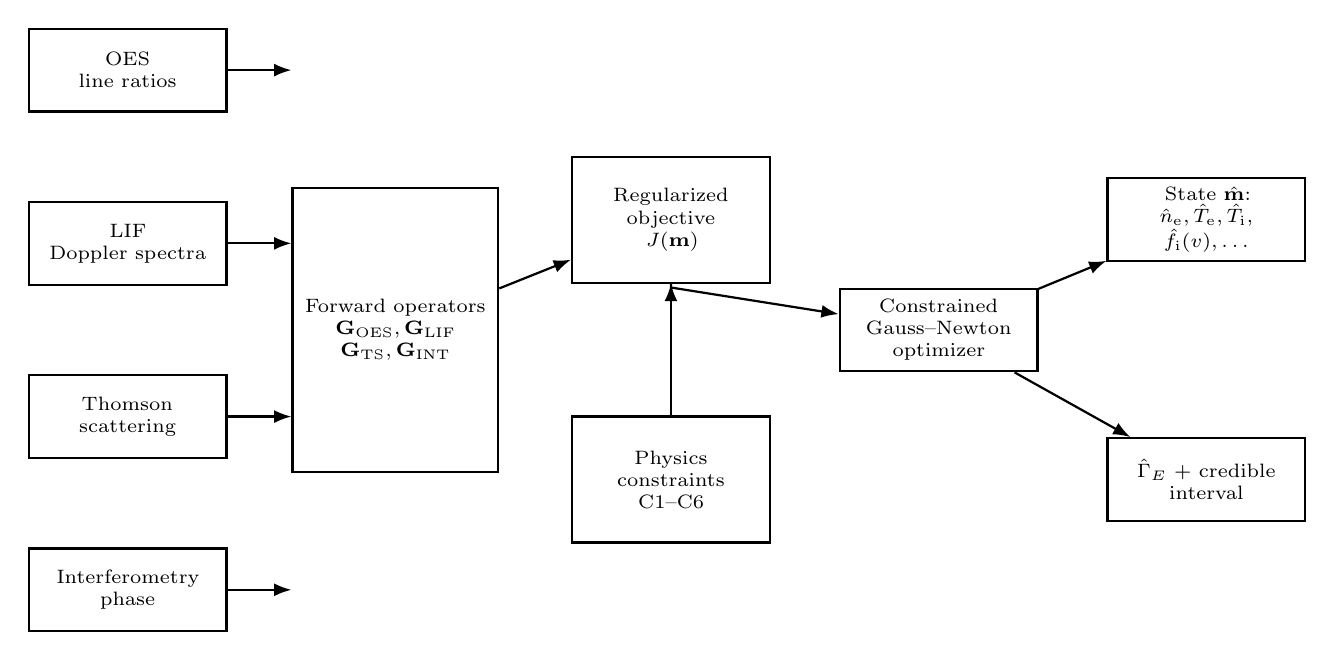
\begin{tikzpicture}[
 box/.style={draw, thick, text width=2.3cm, minimum height=1.05cm, align=center, font=\scriptsize, inner sep=3pt},
 arr/.style={-{Latex[length=2.2mm]}, thick}
]
\node[box] (oes) at (0,3.3) {OES\\line ratios};
\node[box] (lif) at (0,1.1) {LIF\\Doppler spectra};
\node[box] (ts) at (0,-1.1) {Thomson\\scattering};
\node[box] (int) at (0,-3.3) {Interferometry\\phase};
\node[box, text width=2.4cm, minimum height=3.6cm] (fwd) at (3.4,0) {Forward operators\\$\mathbf G_{\mathrm{OES}},\mathbf G_{\mathrm{LIF}}$\\$\mathbf G_{\mathrm{TS}},\mathbf G_{\mathrm{INT}}$};
\node[box, minimum height=1.6cm] (obj) at (6.9,1.4) {Regularized\\objective\\$J(\mathbf m)$};
\node[box, minimum height=1.6cm] (phys) at (6.9,-1.9) {Physics\\constraints\\C1--C6};
\node[box] (opt) at (10.3,0) {Constrained\\Gauss--Newton\\optimizer};
\node[box] (state) at (13.7,1.4) {State $\hat{\mathbf m}$:\\$\hat n_{\mathrm e},\hat T_{\mathrm e},\hat T_{\mathrm i},$\\$\hat f_{\mathrm i}(v),\ldots$};
\node[box] (out) at (13.7,-1.9) {$\hat\Gamma_{E}$ + credible\\interval};
\draw[arr] (oes) -- (fwd.west |- oes);
\draw[arr] (lif) -- (fwd.west |- lif);
\draw[arr] (ts) -- (fwd.west |- ts);
\draw[arr] (int) -- (fwd.west |- int);
\draw[arr] (fwd) -- (obj);
\draw[arr] (phys) -- (obj);
\draw[arr] (obj) -- (opt.north -| obj) -- (opt);
\draw[arr] (opt) -- (state);
\draw[arr] (opt) -- (out);
\end{tikzpicture}
\caption{Schematic (illustrative, not to scale) data flow of the physics-constrained inversion pipeline. Four calibrated optical data streams enter shared forward operators; the resulting predictions are combined with the sheath physics constraints C1--C6 into a single regularized objective, minimized by a constrained Gauss--Newton iteration to yield the joint state estimate $\hat{\mathbf m}$ and the derived ion energy flux $\hat\Gamma_{E}$ with its propagated uncertainty. The diagram is a structural sketch of the algorithm, not a rendering of any measured dataset.}
\label{fig:pci-pipeline}
\end{figure}

\subsection{Stage 1 -- Synchronized acquisition}

The four instruments share a common timebase (phase-locked to the RF drive for the time-resolved formulation), and each acquisition is tagged with timestamp, integration window, and instrument state, so instrument-specific systematics can be modelled explicitly in $\mathbf G$ rather than absorbed into unstructured noise.

\subsection{Stage 2 -- Preprocessing and calibration}

Raw detector output is reduced to calibrated units: OES background-subtracted and instrument-response corrected; LIF corrected for laser power drift and saturation; TS stray-light-subtracted; interferometric phase unwrapped and, where non-uniform, Abel-inverted with a regularized tomographic technique \cite{ref0417}. Each step propagates its own uncertainty into $\boldsymbol\Sigma_{j}$ rather than being treated as exact.

\subsection{Stage 3 -- Initialization from single-diagnostic analytic inversions}

A deliberately crude estimate $\mathbf m^{(0)}$ is formed from the classical analyses -- a Boltzmann-plot $\Te$, an LIF moment fit for $\Ti$ and drift velocity, a Gaussian TS fit for $(\ne,\Te)$, and the Abel-inverted interferometric $\ne$ -- the four ill-posed analyses that motivated this framework. Their role is purely to seed \cref{eq:gauss-newton}; their mutual disagreement is itself diagnostic of the corrections the joint inversion will apply.

\subsection{Stage 4 -- Constrained nonlinear inversion}

The Gauss--Newton (or, for a full posterior, Metropolis-adjusted Langevin/Hamiltonian Monte Carlo) iteration of \cref{eq:gauss-newton} runs from $\mathbf m^{(0)}$ to convergence, C1 via active-set/interior-point, C2--C3 eliminated via \cref{eq:lagrangian}. Where evaluating $\mathbf G_{\mathrm{OES}}$ or $\mathcal T_{\mathrm{sheath}}$ is expensive, a Gaussian-process or neural-network surrogate trained offline is substituted, following accelerated-Bayesian-inference strategies now used for fast profile inversion at stellarator/tokamak scale \cite{ref0728}.

\subsection{Stage 5 -- Regularization-parameter selection}

The weight $\alpha$ is selected, over candidate values, by the corner of the L-curve -- $\big(\log\|\mathbf L(\hat{\mathbf m}(\alpha)-\mathbf m_{\mathrm{ref}})\|_{2},\ \log\|\boldsymbol\Sigma^{-1/2}(\mathbf G(\hat{\mathbf m}(\alpha))-\mathbf d)\|_{2}\big)$ traced as $\alpha$ varies -- or by Morozov's discrepancy principle or generalized cross-validation, standard tools for ill-posed spectroscopic inversion \cite{ref0695} implemented as interchangeable back-ends (\cref{ch15-fig:lcurve}).

\begin{figure}[htbp]
\centering
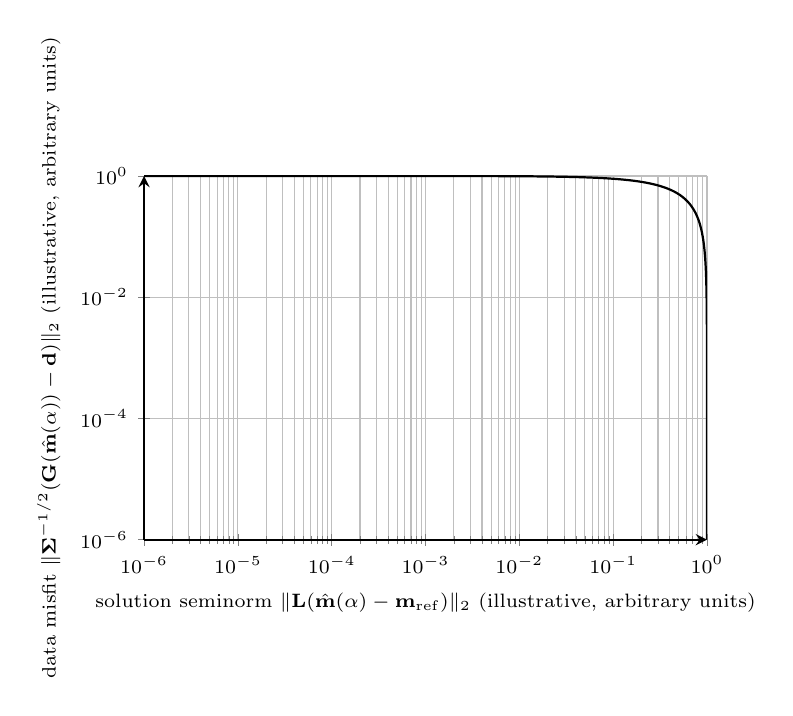
\begin{tikzpicture}
\begin{axis}[
 width=0.72\textwidth,
 height=6.2cm,
 xmode=log, ymode=log,
 xlabel={solution seminorm $\|\mathbf L(\hat{\mathbf m}(\alpha)-\mathbf m_{\mathrm{ref}})\|_{2}$ (illustrative, arbitrary units)},
 ylabel={data misfit $\|\boldsymbol\Sigma^{-1/2}(\mathbf G(\hat{\mathbf m}(\alpha))-\mathbf d)\|_{2}$ (illustrative, arbitrary units)},
 grid=both, axis lines=left, thick,
 label style={font=\scriptsize}, tick label style={font=\scriptsize},
]
\addplot[domain=-3:3,samples=200,black,thick] ({(10^x)^2/((10^x)^2+1)},{1/((10^x)^2+1)});
\end{axis}
\end{tikzpicture}
\caption{Illustrative, schematic L-curve generated from the explicit analytic parametrization $\big(\rho(\alpha),\eta(\alpha)\big)=\big(\alpha^{2}/(\alpha^{2}+1),\,1/(\alpha^{2}+1)\big)$, plotted on logarithmic axes to display the characteristic knee separating the over-smoothed regime (upper left) from the noise-dominated regime (lower right). The curve is a generic mathematical construction used to explain the corner-selection criterion of Stage~5; it does not represent measured or fitted data from any specific inversion.}
\label{ch15-fig:lcurve}
\end{figure}

\subsection{Stage 6 -- Convergence diagnostics and uncertainty quantification}

Convergence is monitored by the KKT residual norm of \cref{eq:kkt1,eq:kkt2}, the relative decrease in $J$, and, once converged, the reduced chi-square $\chi^{2}_{\nu}=2J_{\mathrm{data}}(\hat{\mathbf m})/(q-p)$, near unity for a correctly weighted, non-overfit solution. Where MCMC refines the point estimate, the Gelman--Rubin $\hat R$ statistic and effective sample size provide the acceptance criteria \cite{ref0709,ref0710,ref0727}. The covariance of $\hat{\mathbf m}$ is propagated through the linearization of $\mathcal F$ to give the interval reported for $\hat\Gamma_{E}$,
\begin{equation}
\mathrm{Var}(\hat\Gamma_{E}) \;\approx\; \left(\frac{\partial \mathcal F}{\partial \mathbf m}\right)^{\!\mathsf T}\!\Big[\mathbf J^{\mathsf T}\boldsymbol\Sigma^{-1}\mathbf J + \alpha\mathbf L^{\mathsf T}\mathbf L + \textstyle\sum_{j}\mu_{j}\mathbf D_{j}^{\mathsf T}\mathbf D_{j}\Big]^{-1}\left(\frac{\partial \mathcal F}{\partial \mathbf m}\right) \, , \label{eq:gammaE-variance}
\end{equation}
evaluated at $\hat{\mathbf m}$, the same Gram matrix governing both \cref{eq:gauss-newton} and the stability argument of \cref{sec:pci-objective}.

\section{Assumptions and Their Validation Strategy}
\label{sec:pci-assumptions}

No inversion framework is physics-free, and the credibility of the PCI reconstruction rests on a short list of explicit assumptions, each paired below with a strategy to test rather than merely postulate it. This is deliberately separate from C1--C6: the constraints are relations imposed \emph{within} the estimation, always satisfied at the reconstructed state by construction, whereas the assumptions are conditions under which the entire modelling framework -- choice of forward operators, of which relations qualify as constraints, and of state-space parametrization -- is itself appropriate. A violated constraint shows up as a large residual; a violated assumption is often invisible from within the problem the framework cannot test a premise it was built on.

\begin{enumerate}
\item \textbf{Known atomic/collisional rate data.} $\mathbf G_{\mathrm{OES}}$ needs excitation/de-excitation rate coefficients from an external cross-section database; sensitivity of $\hat{\mathbf m}$ to a bounded perturbation of these is propagated through \cref{eq:gammaE-variance} as an explicit systematic contribution rather than folded into $\boldsymbol\Sigma_{1}$.
\item \textbf{Quasi-one-dimensional sheath geometry.} \Cref{eq:poisson-sheath} assumes a locally planar sheath, tested by comparing chord-averaged interferometry against spatially resolved LIF/OES; where curvature is significant, the framework extends to a 2D-axisymmetric Poisson solve.
\item \textbf{Collisionality regime.} The collisionless/weakly-collisional choice, parametrized by $\mathrm{Kn}_{\mathrm i}$, is validated by a pressure scan (typically \SI{1}{\pascal} to \SI{100}{\pascal}): reconstructed $\mathrm{Kn}_{\mathrm i}$ should track $1/p$ scaling of the mean free path; a systematic departure flags an inadequate closure \cite{ref0077}.
\item \textbf{Steady or periodic-steady operation.} Monitored via residual power in phase bins beyond $N$ and cycle-to-cycle repeatability; a growing high-harmonic residual signals under-resolved nonlinearity or drift requiring the aperiodic formulation.
\item \textbf{Negligible dust/particulate charging and surface contamination.} Checked prior to inversion by independent imaging/process-chemistry evidence; extending C1--C6 to a dusty or electronegative sheath is a model-family choice made upstream, not fitted within the inversion.
\item \textbf{Accurate diagnostic-specific calibration models.} Each $\mathbf G_{j}$ carries instrument constants assumed known independently. Because the problem is over-determined (\cref{sec:pci-overdetermination}), a leave-one-diagnostic-out cross-validation -- refitting from three channels and comparing the withheld channel's prediction to its measurement -- gives an independent test \cite{ref0719}.
\item \textbf{Local linearizability for the Gauss--Newton solver.} Convergence to the global rather than a spurious local minimizer of the non-convex \cref{eq:objective} is not guaranteed a priori; checked via multiple restarts from perturbed $\mathbf m^{(0)}$, agreement with an independent reduced-dimension MCMC exploration, and trust-region step-acceptance monitoring.
\item \textbf{External ground truth.} Where available, $\hat\Gamma_{E}$ is compared against direct, intrusive flux sensors -- dedicated ion-energy-flux sensors \cite{ref0075} and sheath-accelerated secondary-electron flux monitors \cite{ref0078} -- the closest available approximation to independent, non-optical ground truth.
\end{enumerate}

\Cref{tab:assumptions} summarizes this validation matrix.

\begin{table}[htbp]
\centering
\caption{Assumptions underlying the physics-constrained inversion framework and the corresponding validation strategy.}
\label{tab:assumptions}
\begin{tabularx}{\textwidth}{@{}p{4.6cm} X@{}}
\toprule
Assumption & Validation strategy \\
\midrule
Known atomic rate data & Propagate bounded rate-coefficient perturbation through \cref{eq:gammaE-variance} \\
Quasi-1D sheath geometry & Cross-check spatially resolved LIF/OES against chord-averaged interferometry \\
Collisionality regime ($\mathrm{Kn}_{\mathrm i}$) & Pressure scan; test $1/p$ scaling of inferred mean free path \\
Periodic-steady operation & Monitor high-harmonic residual and cycle-to-cycle repeatability \\
No dust/electronegative contamination & Independent process/imaging evidence prior to inversion \\
Diagnostic calibration models & Leave-one-diagnostic-out cross-validation \\
Local linearizability of solver & Multi-restart agreement; reduced-dimension MCMC cross-check \\
Overall pipeline & Comparison against intrusive flux sensors where available \\
\bottomrule
\end{tabularx}
\end{table}

\section{Summary}
\label{sec:pci-summary}

This chapter formalized reconstruction of $\GammaE$ as a single constrained nonlinear estimation problem over a shared plasma/sheath state $\mathbf m$, rather than four sequential, individually ill-posed deconvolutions. The forward model of \cref{sec:pci-forward} showed the four channels probe complementary projections of $\mathbf m$: no single Jacobian block has full column rank, but the stacked, physics-augmented Jacobian generically does. The regularized objective of \cref{sec:pci-objective} makes this over-determination operationally useful, with well-posedness restored by the combined action of a generic prior and the physically motivated constraints; the time-resolved extension of \cref{sec:pci-time} carries the same architecture into RF-periodic and transient regimes where $\GammaE(t)$, not a single number, is the physically meaningful target. The pipeline of \cref{sec:pci-algorithm} and the assumption inventory of \cref{sec:pci-assumptions} are integral to this claim of well-posedness: an inversion that cannot state, test, and revise its own assumptions is not more trustworthy than the single-diagnostic fits it replaces, merely more elaborate.

The central innovation of PCI, and why it is a distinct contribution rather than a routine application of existing IDA machinery \cite{ref0707,ref0712,ref0727}, is its choice of regularizer: rather than a generic smoothness or maximum-entropy prior, it uses the kinetic Bohm criterion, the sheath Poisson/Child--Langmuir relation, and particle- and energy-flux continuity of the plasma--sheath transition itself -- the same conservation and boundary-layer relations developed from first principles earlier in this monograph. Their use as \emph{active constraints inside the estimation}, rather than as passive post-hoc checks, is what converts four separately under-determined optical inversions into one jointly well-posed estimate of $\GammaE$ with quantified, physically defensible uncertainty -- a property the remaining chapters build upon in applying the framework to electric propulsion, plasma etching, and fusion plasma-facing-component contexts. Because PCI treats each of C1--C6 as an auditable residual rather than an implicit assumption baked into a black-box estimator, the reconstructed $\hat{\mathbf m}$ carries a transparent record of which physical relations filled in what the four channels alone could not determine, and by how much each moved the estimate from the raw, unconstrained fit -- the traceability later chapters rely upon in specifying the experimental campaign, uncertainty budget, and validation plan needed to take PCI from algorithmic construction to a demonstrated, defensible measurement of ion energy flux across a real plasma sheath.


\part{Synthesis}
\chapter{Comprehensive Literature Review}
\label{ch:litreview}

Quantifying the ion energy flux delivered to a solid boundary by a bounded plasma sits at the intersection of several traditionally separate sub-disciplines: sheath/presheath theory, non-invasive electron and ion diagnostics, sputtering and erosion physics, and the statistical machinery of inverse problems and Bayesian data fusion. This chapter surveys each theme, establishes its state of the art and open controversies, and draws the threads together to motivate the framework developed later. The organisation is theme-by-theme rather than chronological, since the problem is one of synthesis and no single sub-field supplies a complete answer.

\section{Foundational Sheath and Presheath Theory}

\subsection{The Bohm Criterion: Origins and Kinetic Refinements}

The starting point for any treatment of ion energy flux is the sheath, the boundary layer that forms wherever a plasma contacts a solid surface. Because electrons are far more mobile than ions at equal temperature, the plasma develops a thin, positive layer that confines bulk electrons and accelerates ions toward the surface. The Bohm criterion requires ions to enter the sheath with a directed velocity at least equal to the Bohm speed,
\begin{equation}
u_{\mathrm{B}} = \sqrt{\frac{k_{\mathrm{B}} T_{\mathrm{e}}}{M_{\mathrm{i}}}},
\label{eq:bohm-speed}
\end{equation}
where $T_{\mathrm{e}}$ is the electron temperature and $M_{\mathrm{i}}$ the ion mass. The classical derivation combines ion continuity and energy conservation in a cold, collisionless presheath,
\begin{equation}
n_{\mathrm{i}}(x)\,u_{\mathrm{i}}(x) = n_{0}u_{0}, \qquad
\tfrac{1}{2}M_{\mathrm{i}}u_{\mathrm{i}}^{2}(x) + e\,\phi(x) = \tfrac{1}{2}M_{\mathrm{i}}u_{0}^{2},
\end{equation}
with Boltzmann-distributed electrons, $n_{\mathrm{e}}(x) = n_{0}\exp\!\big(e\phi(x)/k_{\mathrm{B}}T_{\mathrm{e}}\big)$, and Poisson's equation,
\begin{equation}
\frac{\mathrm{d}^{2}\phi}{\mathrm{d}x^{2}} = -\frac{e}{\epsilon_{0}}\big(n_{\mathrm{i}}(x) - n_{\mathrm{e}}(x)\big).
\label{ch23-eq:poisson}
\end{equation}
Expanding the right-hand side of Eq.~\eqref{ch23-eq:poisson} to first order in $\phi$ shows a monotonic space-charge solution exists only if $u_{0} \ge u_{\mathrm{B}}$, recovering Eq.~\eqref{eq:bohm-speed} as Bohm originally argued and as later placed on a rigorous kinetic footing \cite{ref0001}. The kinetic generalisation replaces the cold-fluid ion population with an arbitrary distribution $f_{\mathrm{i}}(v)$ entering the sheath edge, giving the integral form of the criterion,
\begin{equation}
\int_{0}^{\infty} \frac{f_{\mathrm{i}}(v)}{v^{2}}\,\mathrm{d}v \;\le\; \frac{n_{\mathrm{i}0} M_{\mathrm{i}}}{k_{\mathrm{B}} T_{\mathrm{e}}},
\label{eq:kinetic-bohm-review}
\end{equation}
which reduces to Eq.~\eqref{eq:bohm-speed} for a mono-energetic beam and exposes the outsized role of the low-velocity tail of $f_{\mathrm{i}}(v)$: ions barely satisfying the criterion contribute disproportionately, and a fluid estimate tracking only moments can be invalidated by that tail. How the presheath field should behave as collisionality vanishes remains disputed, including whether the criterion is an equality or an inequality.

Extensions to warm ions, multiply charged species, secondary electron emission, and non-Maxwellian electrons are well developed \cite{ref0004}, and reformulations avoiding the singular sheath-edge field in the strict Bohm limit have clarified presheath-sheath asymptotic matching \cite{ref0009}. Whether a single criterion applies universally across collisionality, magnetisation, electronegativity, and non-thermal populations remains open \cite{ref0015}.

\subsection{Presheath Structure and Collisional Effects}

The presheath is the quasi-neutral region, typically many Debye lengths in extent, over which ions accelerate from thermal bulk velocity to the Bohm speed. Its structure depends on the dominant momentum-loss mechanism: ionisation-driven presheaths in weakly ionised discharges, collision-dominated presheaths at higher pressure, and geometric presheaths set by confinement scale. Two-fluid treatments show the presheath-sheath boundary is a matter of definition rather than a sharp discontinuity \cite{ref0023}; the sheath is more properly the limit where the Debye length matches the density-gradient scale, requiring matched asymptotic expansions to connect the regions \cite{ref0013}. Collisional presheaths, where ion-neutral collisions dominate the friction against acceleration, modify the effective sheath-edge velocity and, in the fully collisional limit, replace the kinetic Bohm criterion with a fluid drift-diffusion balance \cite{ref0024}. Charge-exchange collisions reducing wall-incident ion flux have been treated as an explicit correction to the collisionless estimate \cite{ref0077}.

\subsection{Magnetised and Multi-Species Generalisations}

When a magnetic field intersects the boundary obliquely, the presheath acquires a further structure — the magnetic presheath or Chodura layer — over which ions turn from motion along the field line to motion along the density gradient, satisfying a magnetised Bohm criterion at the entrance to the Debye sheath \cite{ref0017}. This layer, of order the ion Larmor radius, sits between the electrostatic sheath and the longer collisional/ionisation presheath, giving the boundary a three-scale structure whenever the field is not normal to the surface. In multi-ion-species plasmas, individual species need not each satisfy their own marginal condition — only the species-summed criterion must hold, confirmed via laser-induced-fluorescence measurements of two ion species approaching the sheath edge together \cite{ref0329}. In electronegative and dusty plasmas, negative ions or charged dust grains modify electron screening and can shift the marginal Bohm speed from the single-species value.

\subsection{Open Questions and Controversies}

Despite more than seven decades of development since Bohm's original argument, no fully general theory of the plasma-sheath transition commands unanimous acceptance \cite{ref0015}. Disagreements persist over the sheath-edge field singularity, whether an inequality or marginal equality is physically realised in weakly collisional plasmas, the correct closure for the ion energy equation in fluid models, and how continuum-kinetic solvers should implement boundary conditions. These are not academic disputes: any attempt to quantify ion energy flux from first principles inherits them, since the flux is a moment of $f_{\mathrm{i}}(v)$ evaluated precisely where the theory is least settled.

\subsection{Model Hierarchies: Fluid, Kinetic, and Particle-Based Solution Strategies}

These disagreements reflect the fact that the sheath-presheath problem admits three distinct solution classes on different points of the accuracy-versus-cost curve, with no preferred hierarchy for coupling them. Fluid (moment) models close the ion continuity and momentum equations with an assumed equation of state, cheap enough for reactor-scale simulation but discarding the low-order velocity-space structure Eq.~\eqref{eq:kinetic-bohm-review} shows to be consequential \cite{ref0023}. Fully kinetic particle-in-cell methods retain the complete distribution function but introduce statistical noise controlled only through particle-count scaling, with explicit time-stepping tying affordable domain size to the Debye length and plasma frequency \cite{ref0631}. Continuum-kinetic solvers discretising the Vlasov equation on a phase-space grid eliminate particle noise at the cost of memory scaling unfavourably with resolved velocity-space dimensions \cite{ref0659}. Practical recipes for patching a fluid or hybrid solution to a kinetic sheath treatment offer a pragmatic middle path \cite{ref0012}. No consensus exists on which hierarchy suffices for a given accuracy target, motivating the approach adopted here: the model hierarchy itself is treated as a further source of epistemic uncertainty, quantified alongside measurement noise.

\section{Time-Varying and Radio-Frequency Sheaths}

\subsection{RF Sheath Models and Ion Transit-Time Effects}

Radio-frequency (RF) capacitively coupled plasmas present a qualitatively different sheath problem: the sheath boundary oscillates at the driving frequency (typically $\SI{13.56}{\mega\hertz}$ or a harmonic), and the ion response depends on the ratio of the RF period to the ion transit time. In the low-frequency limit ions respond quasi-statically, producing a bimodal energy distribution at the electrode; in the high-frequency limit ions respond only to the time-averaged field, producing a narrow, quasi-mono-energetic distribution \cite{ref0055}. Analytic RF sheath models — collisionless, collisional, hybrid — bridge these limits, predicting sheath voltage, thickness, and ion energy distribution versus frequency, pressure, and waveform \cite{ref0038}. The classical Child-Langmuir space-charge-limited current law for a static planar diode,
\begin{equation}
J = \frac{4}{9}\,\epsilon_{0}\sqrt{\frac{2e}{M_{\mathrm{i}}}}\,\frac{V^{3/2}}{s^{2}},
\label{ch23-eq:child-langmuir}
\end{equation}
where $V$ is the sheath voltage drop and $s$ the instantaneous sheath thickness, remains the backbone of most time-averaged RF sheath models, with $s(t)$ evolving self-consistently with the RF voltage.

\subsection{Kinetic and Particle-in-Cell Descriptions of RF Sheath Dynamics}

Because ion transit times are frequently comparable to the RF period, fully kinetic treatments are needed to capture the resulting non-Maxwellian, bimodal, or multi-modal energy distributions. Kinetic and hybrid PIC/Monte-Carlo simulations show that self-bias voltage, secondary electron emission, and waveform harmonic content all reshape the RF sheath beyond what analytic models capture \cite{ref0637}. Sawtooth and other tailored voltage waveforms control the harmonic content of the sheath modulation and hence the resulting IEDF \cite{ref0043}. Kinetic simulations of the intermediate-frequency regime have quantified how the IEDF transitions continuously between the bimodal and narrow limits \cite{ref0040}.

\subsection{Electrical Asymmetry and Ion Energy Control}

A major practical development is the deliberate exploitation of waveform tailoring to decouple ion flux and ion energy at a substrate, historically impossible in a single-frequency discharge \cite{ref0105}. The electrical asymmetry effect, whereby a phase-shifted dual- or multi-frequency waveform breaks the powered/grounded electrode symmetry, produces a DC self-bias tunable to shift mean ion energy while approximately preserving flux \cite{ref0106}, underlying essentially all modern "tailored ion energy distribution" process technology \cite{ref0105}. This body of work is almost entirely oriented toward control — producing a desired IEDF at a substrate — rather than toward inferring delivered energy flux from external, non-invasive measurements.

\section{Ion Energy Flux at Plasma Boundaries}

\subsection{Definition and the Governing Flux Integral}

The central quantity throughout this monograph is the ion energy flux delivered to a surface, the third velocity moment of the ion distribution at the sheath-plasma boundary,
\begin{equation}
\Gamma_{E} = \int_{0}^{\infty} \tfrac{1}{2} M_{\mathrm{i}} v^{2}\, v\, f_{\mathrm{i}}(v)\,\mathrm{d}v ,
\label{ch23-eq:energy-flux-def}
\end{equation}
with units of power per unit area. For a cold-ion presheath entering at exactly the Bohm speed and accelerated through the sheath drop $\Delta V_{\mathrm{sh}}$, Eq.~\eqref{ch23-eq:energy-flux-def} reduces to the engineering form,
\begin{equation}
\Gamma_{E} \approx \Gamma_{\mathrm{i}}\Big(\tfrac{1}{2}k_{\mathrm{B}}T_{\mathrm{e}} + e\,\Delta V_{\mathrm{sh}}\Big), \qquad \Gamma_{\mathrm{i}} = n_{\mathrm{s}} u_{\mathrm{B}},
\label{eq:energy-flux-eng}
\end{equation}
where $n_{\mathrm{s}}$ is the sheath-edge ion density and $\Gamma_{\mathrm{i}}$ the particle flux; the $\tfrac{1}{2}k_{\mathrm{B}}T_{\mathrm{e}}$ term reflects presheath-acquired energy, while $e\,\Delta V_{\mathrm{sh}}$ dominates for typical sheath voltages several times $T_{\mathrm{e}}$ in electron-volts. Equation~\eqref{eq:energy-flux-eng} presumes a mono-energetic, collisionless, single-species traversal — routinely violated — and prior knowledge of $n_{\mathrm{s}}$, $T_{\mathrm{e}}$, and $\Delta V_{\mathrm{sh}}$, each a diagnostic challenge in itself. Fluid models carrying the full ion energy spectrum through the sheath capture how a broadened or bimodal edge distribution propagates into the delivered flux \cite{ref0083}, and non-Maxwellian generalisations have been derived for Kappa-distributed electrons relevant to space plasmas \cite{ref0090}.

\subsection{Sensors and In Situ Flux Measurement}

Because Eq.~\eqref{ch23-eq:energy-flux-def} cannot generally be evaluated from first principles with process- or lifetime-relevant accuracy, dedicated flux sensors have been developed to measure $\Gamma_{E}$ directly, typically via a thermally isolated collector whose temperature rise is calibrated against incident power flux \cite{ref0075}, related to heat-flux microsensors for calorimetric measurement of interaction power density \cite{ref0175}. In plasma immersion ion implantation, sheath-accelerated secondary electron currents serve as a non-invasive proxy for instantaneous ion flux \cite{ref0078}. Direct wafer-surface heat-flux measurements during reactive-ion-etch processing provide a further empirical benchmark \cite{ref0080}. A consistent theme emerges: every practical sensor perturbs the plasma, is restricted to a specific geometry or waveform, or returns an integrated, energy-unresolved quantity.

\subsection{Collisional and Non-Maxwellian Corrections to the Flux}

Realistic sheaths are neither perfectly collisionless nor Maxwellian, and both departures modify Eq.~\eqref{eq:energy-flux-eng} substantially. Ion-neutral collisions broaden and skew the arriving ion energy distribution, captured in fluid and hybrid sheath models tracking the full spectrum rather than assuming ballistic acceleration \cite{ref0074}. Magnetised sheaths make delivered ion energy depend on the field-surface angle, since only the field-aligned velocity component is accelerated \cite{ref0088}. Data-driven closures for sheath heat flux, extracted from kinetic simulation data via symbolic regression, suggest the fluid-closure problem may be tractable empirically \cite{ref0101}. System-level power-balance accounting in fusion plasmas illustrates the stakes of an accurate flux estimate at reactor-engineering level \cite{ref0093}.

\section{Ion Energy Distribution Functions}

\subsection{Analytic and Numerical IEDF Models}

The ion energy distribution function (IEDF), $f_{\mathrm{i}}(E)$, is the full energy-resolved generalisation of the flux integral of Eq.~\eqref{ch23-eq:energy-flux-def}, connecting sheath theory to both diagnostics and materials response, since sputtering yield is itself strongly energy-dependent. In the collisionless, single-frequency RF limit, the IEDF at the powered electrode takes a bimodal "saddle" shape, with peaks at $E_{\min}$ and $E_{\max}$ separated by an amount scaling inversely with driving frequency and ion transit time: longer transit relative to the RF period narrows rather than widens the spread. The low-energy peak corresponds to ions near the minimum instantaneous sheath voltage during transit, the high-energy peak to those near the maximum \cite{ref0123}, generalised since to arbitrary driving frequency and Kappa-distributed suprathermal electrons \cite{ref0123}. A rigorous kinetic boundary condition connecting the bulk ion velocity distribution to fluid moments replaces the ad hoc mono-energetic assumption in most fluid models \cite{ref0119}.

\subsection{Diagnostic Reconstruction of the IEDF}

Because $f_{\mathrm{i}}(E)$ cannot generally be measured directly at the sheath edge, indirect reconstruction strategies dominate. Retarding field energy analysers (RFEAs), measuring current transmitted through biased grids versus retarding potential, remain the most widely deployed direct IEDF technique, including through RF- or pulse-biased sheaths where the response must be synchronised to the drive waveform \cite{ref0540}. Planar laser-induced-fluorescence systems extend this to a full two-dimensional spatial map \cite{ref0304}. In electric propulsion, ion energy diagnostics of the Hall-thruster exhaust plume make the IEDF a mission-critical quantity governing thrust efficiency and erosion risk \cite{ref0114}, situated within its principal application by the broader ion-thruster review \cite{ref0115}.

\section{Sputtering, Erosion, and Surface Yield Physics}

\subsection{Binary-Collision Theory and Empirical Yield Laws}

The ion energy flux delivered to a surface, quantified via Eqs.~\eqref{ch23-eq:energy-flux-def}--\eqref{eq:energy-flux-eng}, matters because it drives physical sputtering: ejection of surface atoms via momentum transfer from incident ions. The theoretical foundation is linear-cascade binary-collision theory, in which an incident ion transfers momentum through a cascade of elastic nuclear collisions, a fraction of which reach the surface with enough outward momentum to overcome the binding energy \cite{ref0143}, yielding the Sigmund sputtering-yield formula, which for normal incidence and energies well above threshold takes the form
\begin{equation}
Y(E) = \Lambda\, S_{\mathrm{n}}(E),
\end{equation}
where $\Lambda$ is a materials constant proportional to the inverse surface binding energy and $S_{\mathrm{n}}(E)$ the nuclear stopping cross section, expressible through the reduced (Lindhard) energy $\varepsilon$. The Bohdansky formula introduces a threshold energy $E_{\mathrm{th}}$ below which sputtering vanishes, reproducing the low-energy roll-off,
\begin{equation}
Y(E) = Q\, S_{\mathrm{n}}(\varepsilon) \left[1 - \left(\frac{E_{\mathrm{th}}}{E}\right)^{2/3}\right]\left[1 - \frac{E_{\mathrm{th}}}{E}\right]^{2},
\label{ch23-eq:bohdansky}
\end{equation}
with $Q$ a target-dependent constant, illustrated schematically in Fig.~\ref{fig:sputter-yield}. Direct experimental sputtering-yield measurements under controlled ion-beam and plasma bombardment \cite{ref0152} remain the principal calibration source for $\Lambda$, $Q$, and $E_{\mathrm{th}}$, and comprehensive treatments of the collision-cascade physics remain the reference framework for newer molecular-dynamics and machine-learning yield models \cite{ref0144}. The single-parameter yield curve is at best leading-order; energy- and angle-resolved sputtering, driven by the full IEDF rather than a single characteristic energy, is the physically correct generalisation and precisely the coupling this monograph seeks to exploit.

\begin{figure}[htbp]
\centering
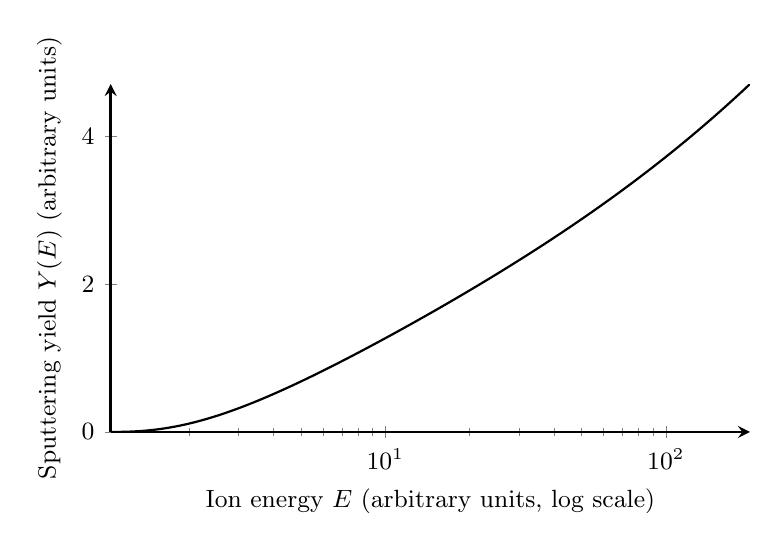
\begin{tikzpicture}
\begin{axis}[
 width=0.8\linewidth, height=6cm,
 xlabel={Ion energy $E$ (arbitrary units, log scale)},
 ylabel={Sputtering yield $Y(E)$ (arbitrary units)},
 xmode=log,
 domain=1.05:200,
 samples=200,
 axis lines=left,
 grid=none,
 line width=0.9pt,
 every axis plot/.append style={color=black},
 tick label style={font=\small},
 label style={font=\small},
]
\addplot[black, thick] { (1 - (1/x)^(2/3)) * (1 - 1/x)^2 * (x^0.3) };
\end{axis}
\end{tikzpicture}
\caption{Schematic, illustrative plot of the analytic Bohdansky-type sputtering-yield law of Eq.~\eqref{ch23-eq:bohdansky}, normalised to a unit threshold energy $E_{\mathrm{th}}=1$ and plotted against a simplified power-law stand-in for the nuclear stopping cross section $S_{\mathrm{n}}(\varepsilon)\propto E^{0.3}$. The curve illustrates the functional form only and does not represent measured or fitted data for any specific ion-target combination.}
\label{fig:sputter-yield}
\end{figure}

\subsection{Erosion Measurement and Long-Term Lifetime Assessment}

Translating an instantaneous sputtering yield into cumulative erosion depth or mass-loss rate requires integrating it against the full, time-dependent, energy- and angle-resolved ion flux over a component's operational lifetime — a direct application of the problem addressed here. In fusion plasma-facing-component research, the gross and net erosion balance of tungsten and other divertor materials has been measured and modelled extensively \cite{ref0158}, and dedicated material-testing facilities expose candidates to controlled ion energy fluxes for erosion-rate calibration \cite{ref0586}. Comparisons of predicted erosion, using yield laws such as Eq.~\eqref{ch23-eq:bohdansky}, against measured erosion of tungsten coatings reveal discrepancies from redeposition, morphology evolution, and mixed-species bombardment not captured by the flat-surface formula \cite{ref0593}. In electric propulsion, channel-wall erosion in Hall-effect thrusters, driven by near-wall sheath impact on the ceramic discharge channel, has been measured directly via laser-induced fluorescence of sputtered wall material \cite{ref0454} and reviewed as the principal life-limiting mechanism for this thruster class \cite{ref0440}. Surface characterisation techniques — interferometry, thickness measurement, witness-coating methods — offer post-exposure routes trading resolution against invasiveness. The gap mirrors that for flux sensing: erosion measurement is almost universally destructive/post-hoc, motivating a forward-predictive alternative.

\section{Plasma-Material Interaction and Heat Flux}

The ion energy flux problem generalises to total power deposition — ion kinetic energy, recombination energy, and electron heat flux combined — onto a plasma-facing surface. High-heat-flux plasma-material interaction has been studied intensively in fusion, where transient events such as edge-localised modes and disruptions deposit power densities orders of magnitude above steady state, driving melt-layer formation, cracking, and rapid material loss on tungsten and molybdenum components \cite{ref0581}. Physical modelling of the resulting vapour-shielding effect, where ablated material absorbs and re-radiates incident heat flux, illustrates the strongly nonlinear, self-limiting character of extreme plasma-material interaction \cite{ref0176}. Materials-screening studies rank candidates against combined erosion and heat-flux-tolerance criteria \cite{ref0189}, while broader reviews treat the two as jointly limiting constraints \cite{ref0190}. Diagnostics here include direct heat-flux microsensors \cite{ref0175} and laser Thomson scattering adapted for divertor and limiter edge plasmas \cite{ref0383}.

\section{Electrostatic Probe Diagnostics}

Langmuir probes remain the most widely deployed diagnostic for local electron temperature and density in low-temperature and processing plasmas, feeding directly into the Bohm-speed and sheath-voltage estimates of Eq.~\eqref{eq:energy-flux-eng}. The classical single-probe I-V characteristic analysis, extracting electron temperature from the semi-logarithmic slope of the electron-retarding-region current, has been refined through fitting procedures reducing sensitivity to probe contamination, RF pickup, and non-Maxwellian distortion \cite{ref0217}. Gyrofluid-simulation-based analyses of probe-measured temperatures quantify biases inherent to the fluid interpretation of probe traces \cite{ref0194}. Comparisons of Langmuir-probe-derived $T_{\mathrm{e}}$ and $n_{\mathrm{e}}$ against OES \cite{ref0237} and Thomson scattering \cite{ref0355} provide essential cross-validation, though systematic offsets persist in magnetised or strongly non-Maxwellian plasmas. In the fusion-edge context, Langmuir-probe arrays remain the primary means of characterising the electron energy distribution and plasma potential at the tokamak boundary \cite{ref0213}. A recommended-practice document for electric-propulsion testing codifies probe construction, sweep circuitry, and data interpretation for thruster plasmas \cite{ref0226}.

\section{Optical Emission Spectroscopy and Collisional-Radiative Modeling}

Optical emission spectroscopy (OES) offers a non-invasive alternative to probe-based diagnostics, inferring electron temperature and density from relative intensities of atomic or ionic emission lines. Because excited-state populations are set by a balance of excitation, de-excitation, ionisation, and radiative decay, quantitative interpretation of OES line ratios requires a collisional-radiative (CR) model rather than a corona- or LTE-equilibrium assumption \cite{ref0260}. Line-ratio methods based on helium metastable and resonance transitions are a well-validated CR-model application, cross-checked against probe and Thomson-scattering measurements \cite{ref0266}. Argon CR models have received sustained development given argon's ubiquity as a processing gas \cite{ref0245}, including Bayesian frameworks propagating atomic-data uncertainty through to inferred $T_{\mathrm{e}}$ and $n_{\mathrm{e}}$ \cite{ref0275}.

OES has also extracted time-resolved electron temperature evolution in Hall thrusters synchronised to discharge oscillations \cite{ref0256}. Tomographic reconstruction of the spatially resolved electron-property field from line-integrated OES chords has been demonstrated for the Hall-thruster acceleration region \cite{ref0257}. Real-time OES-based process monitoring has become standard for closed-loop control of deposition and etch processes \cite{ref0553}.

\section{Laser-Induced Fluorescence and Ion Velocity Distribution Function Measurement}

Laser-induced fluorescence (LIF) occupies a uniquely important position because, unlike OES or Langmuir probes, it provides a non-invasive, spatially and spectrally resolved measurement of the ion velocity distribution function itself, not only its low-order moments. A narrow-linewidth tunable laser is scanned across a Doppler-broadened absorption transition of a metastable ion state, and fluorescence intensity versus detuning maps the projection of $f_{\mathrm{i}}(v)$ along the laser direction \cite{ref0292}, applied extensively to characterise ion dynamics near the sheath boundary \cite{ref0329} and providing the most direct experimental window onto the kinetic quantities entering Eq.~\eqref{eq:kinetic-bohm-review} and Eq.~\eqref{ch23-eq:energy-flux-def}. Planar and tomographic LIF implementations extend the single-point measurement to a full multi-dimensional map, of particular value in electric-propulsion plumes \cite{ref0328}.

Within electric propulsion, LIF has become the diagnostic of record for ion velocity distributions in Hall-thruster channels and plumes, revealing multi-population structure — counter-streaming and near-wall populations — invisible to bulk flux or probe measurements \cite{ref0322}. Comprehensive reviews of the LIF technique provide the methodological foundation this monograph builds on \cite{ref0347}.

\section{Thomson Scattering and Interferometric Density Diagnostics}

Incoherent Thomson scattering provides a first-principles, calibration-independent measurement of the local electron velocity distribution, and hence $T_{\mathrm{e}}$ and $n_{\mathrm{e}}$, through the Doppler broadening and intensity of light scattered from free electrons by an intense probe laser \cite{ref0354}. Its principal limitation — an extremely small scattering cross section requiring high electron density or a very high-power laser — has been addressed through portable, temporally resolved systems for low-density plasmas \cite{ref0357}, and spatially resolved implementations mapping electron properties across a magnetically shielded Hall thruster's acceleration region \cite{ref0356}. Because it measures the electron distribution directly without an atomic model, Thomson scattering provides an independent cross-check against Langmuir-probe and OES/CR-model-derived properties \cite{ref0355}; comparisons across all three quantify the achievable agreement and residual discrepancies from probe perturbation or atomic-data uncertainty.

Microwave and laser interferometry complement Thomson scattering with a line-integrated but simple, robust electron-density measurement via the plasma-induced phase shift of a probe beam. Multi-chord configurations enable coarse tomographic resolution of the density profile \cite{ref0399}, valuable for the fusion-edge profiles discussed later. Dispersion-interferometer configurations, suppressing sensitivity to vibration and beam steering by combining two harmonically related probe frequencies, have been deployed in pulsed-power and transmission-line contexts requiring high time resolution \cite{ref0417}.

\section{Electric Propulsion: Erosion and Diagnostics of Hall and Ion Thrusters}

Electric propulsion is one of the most demanding, thoroughly instrumented application domains for ion energy flux quantification, since Hall-effect and gridded ion thrusters rely on a confined sheath to accelerate ions, and both suffer life-limiting erosion driven by the ion energy flux incident on discharge-channel walls or accelerator grids. In Hall thrusters, near-wall ion bombardment of the ceramic discharge channel is the dominant erosion mechanism, and two-dimensional hybrid and fully kinetic PIC models predict erosion rates and lifetime from first principles \cite{ref0433}. Reviews of Hall-thruster erosion synthesise decades of experience, from empirical scaling laws to self-consistent kinetic prediction \cite{ref0440}. Magnetic shielding — deflecting the bulk of the energetic ion flux away from the channel wall — has transformed erosion-limited lifetime, and near-wall transport in shielded configurations continues to be studied \cite{ref0425}. In gridded ion thrusters, accelerator-grid erosion driven by charge-exchange bombardment, rather than direct beam-ion impact, has been modelled using dedicated plume codes validated against measured patterns \cite{ref0463}.

Diagnostic methodology specific to electric propulsion has matured into its own recommended-practice literature, spanning Langmuir and emissive probe protocols \cite{ref0226}, RFEA design for plume ion-energy characterisation \cite{ref0490}, and reviews of the instrumentation suite for ground-test and in-flight packages \cite{ref0506}. A well-documented complication is facility background-gas pressure, which introduces charge-exchange pathways absent in space and biases measured performance and erosion \cite{ref0461} — a practical manifestation of the same collisional-correction issue treated theoretically above.

\section{Plasma Etching and Semiconductor Process Diagnostics}

Reactive-ion and plasma etching depend critically on the ion energy delivered to the wafer surface, since etch rate, selectivity, and profile anisotropy are strongly and often non-monotonically dependent on the incident ion energy distribution. Model-based coupling of ion energy flux to spatially resolved etch-profile evolution, convolving the local angle- and energy-dependent etch yield with evolving surface topography, has been developed for collisionless sheaths typical of low-pressure etch tools \cite{ref0074}. Foundational reviews of plasma etching technology situate the problem within the semiconductor-manufacturing context, covering etch mechanisms, mask selectivity, and the etch-rate/anisotropy trade-off \cite{ref0536}. Independent control of ion density and bombardment energy — via dual-frequency schemes related to the electrical-asymmetry techniques above — remains a central goal of process-tool design, since selectivity and damage thresholds impose conflicting constraints on the acceptable energy window \cite{ref0539}.

Complementary in situ diagnostics include broader treatments of plasma diagnostics for real-time monitoring and closed-loop control \cite{ref0553}. Direct measurement of the ion energy distribution using retarding-potential analysers, in RF and pulsed-DC configurations, provides the empirical benchmark for the model-based predictions above \cite{ref0540}. Despite its maturity and commercial stakes, this literature remains largely tool- and recipe-specific; a generalisable framework transferring across chemistries and geometries is an opportunity this monograph addresses.

\section{Fusion Plasma-Wall Interaction and the Tokamak Edge}

The scrape-off layer (SOL) and divertor regions of a magnetically confined fusion device present perhaps the most consequential real-world instance of the ion-energy-flux problem, since divertor heat and particle flux directly govern component lifetime and, at reactor scale, the feasibility of steady-state operation. The SOL heat-flux width — the radial decay length over which heat flux is deposited onto the divertor target — is the subject of intensive multi-machine scaling studies and continued controversy over extrapolation to reactor parameters. Power-deposition models spanning simple convective formulations through to turbulence simulations resolving divertor heat load during thermal-quench transients illustrate the same fluid-versus-kinetic tension already encountered in sheath theory, now at tokamak-engineering scale \cite{ref0605}. High-heat-flux testing facilities reproducing ITER-relevant divertor loading on candidate mock-ups provide the essential validation layer \cite{ref0581}.

SOL turbulence — intermittent, filamentary blob transport dominating cross-field transport near the SOL — has been characterised through gyrokinetic and reduced fluid simulation \cite{ref0605} and through direct filament tracking using fast visible imaging and probe arrays on MAST and Alcator C-Mod \cite{ref0600}. RFEA measurements of ion temperature at the divertor target provide one of the few direct, energy-resolved constraints on the flux actually delivered to a tokamak surface, rather than inferred via upstream measurements and a sheath-transmission model \cite{ref0610}.

\section{Kinetic Theory and Particle-in-Cell Simulation of the Sheath}

Fully kinetic simulation, whether via Lagrangian particle-in-cell (PIC) methods or Eulerian continuum-kinetic (Vlasov) solvers, provides the most rigorous route to computing $f_{\mathrm{i}}(v)$ self-consistently across the presheath-sheath system without invoking fluid closure assumptions. The original fully kinetic, self-consistent PIC treatment of the collisionless plasma-sheath region established the basic simulation methodology still in wide use, resolving the sheath potential profile, ion velocity distribution, and Bohm-criterion satisfaction from first principles \cite{ref0631}. Subsequent PIC studies have extended this to magnetised sheaths \cite{ref0633} and ion-ion (electronegative or dual-species) sheath and presheath structure \cite{ref0655}. Continuum-kinetic (Eulerian, discontinuous-Galerkin) solvers, discretising the Vlasov equation on a phase-space grid rather than sampling with finite-weight particles, eliminate PIC's statistical noise at the cost of substantially higher computational and memory demand, and have resolved fine structure in the sheath-edge ion distribution — including the low-velocity tail central to Eq.~\eqref{eq:kinetic-bohm-review} — with a fidelity difficult for particle methods \cite{ref0659}. The Tonks-Langmuir model — an exactly solvable, ionisation-dominated kinetic presheath model — remains the canonical benchmark for numerical kinetic solvers, and continued debate over whether the kinetic Bohm criterion is an assumption or a derivable theorem within it shows that even this idealised problem retains open questions \cite{ref0665,ref0666}.

\section{Inverse Problems, Bayesian Inference, and Multi-Diagnostic Data Fusion}

The final theme is methodological rather than purely physical: reconstructing an underlying quantity — the sheath-edge ion energy distribution or the delivered energy flux — from indirect, noisy, incomplete measurements. Classical regularisation theory, most prominently Tikhonov regularisation, stabilises the otherwise ill-posed inversion of a convolved measurement back to the underlying resolved quantity, applied to tomographic laser-absorption spectroscopy problems structurally analogous to plasma-diagnostic tomography \cite{ref0677}. Related strategies — total-variation penalisation, iterative regularisation, and regularisation-parameter selection — have been developed across imaging and spectroscopy inverse problems \cite{ref0692}, a mature toolkit transferable to plasma-diagnostic inversion. Optical tomography of plasma emission, reconstructing a spatially resolved emissivity field from limited chordal measurements, is a direct instance of the same ill-posed problem, addressed through both classical algebraic reconstruction and Bayesian tomographic frameworks \cite{ref0685}.

Bayesian inference has emerged as the dominant modern methodology for principled multi-diagnostic data fusion in plasma physics, treating each diagnostic as an imperfect, noisy observation of a shared plasma state combined through a rigorously specified joint likelihood and prior \cite{ref0706}. Integrated data analysis frameworks of this type have been deployed extensively at major tokamak facilities, fusing Thomson scattering, interferometry, and magnetic equilibrium reconstruction into a single self-consistent kinetic-profile inference for ITER operation \cite{ref0706}, and comprehensive reviews catalogue both the methodology's successes and its remaining computational-cost and prior-specification challenges \cite{ref0710}. Bayesian model selection has been applied to Thomson-scattering spectral analysis to discriminate between competing models on a rigorous statistical footing rather than by visual inspection \cite{ref0684}, and analogous frameworks have been applied to combined OES/CR-model inference, propagating atomic-data uncertainty through to inferred electron properties \cite{ref0275}. In electric propulsion, Bayesian calibration and uncertainty quantification of Hall-thruster models against multi-diagnostic measurement sets illustrates this methodology's applicability to the erosion- and flux-relevant problems above \cite{ref0719}. The broader review of data-driven plasma science underscores the growing consensus that principled uncertainty quantification, rather than point-estimate reporting, should be the standard for any inferred plasma quantity \cite{ref0711}.

\section{Synthesis: Cross-Theme Connections to the Proposed Framework}

Read individually, the fifteen themes surveyed above appear as largely independent literatures, each with its own journals and vocabulary. Read together, a single connected chain becomes visible, and it is this chain the framework developed in this monograph seeks to instantiate end to end. Sheath and presheath theory supplies the first-principles relationship between bulk-plasma parameters ($T_{\mathrm{e}}$, $n_{\mathrm{e}}$, $f_{\mathrm{i}}(v)$) and the sheath-edge ion flux and energy, formalised in the Bohm criterion of Eq.~\eqref{eq:bohm-speed} and its kinetic generalisation, Eq.~\eqref{eq:kinetic-bohm-review}. Time-varying and RF sheath theory extends this to the driven boundary conditions of essentially all technologically deployed plasmas, introducing the Child-Langmuir scaling of Eq.~\eqref{ch23-eq:child-langmuir} and the bimodal IEDF structure. The ion-energy-flux and IEDF literatures then define the target quantity itself — Eqs.~\eqref{ch23-eq:energy-flux-def}--\eqref{eq:energy-flux-eng} — and expose the central practical difficulty: existing sensors either perturb the measurement, are geometry- or waveform-specific, or return only an energy-integrated quantity.

The diagnostic themes — electrostatic probes, OES/CR modelling, laser-induced fluorescence, and Thomson scattering/interferometry — supply the raw, non-invasive observables from which the bulk-plasma inputs to the sheath theory can be reconstructed. Each measures a different moment of the underlying plasma state, with its own noise, resolution, and systematic-error structure; the sustained cross-comparison literature between the three documents both the value and the limits of any single diagnostic in isolation. This is precisely the gap the inverse-problems and data-fusion literature closes: rigorous, uncertainty-aware combination of multiple imperfect channels into a single, self-consistent estimate of the plasma state and, via the sheath theory above, of the ion energy flux itself.

The consequences of an accurately quantified flux are made concrete by the applied themes: sputtering and erosion physics, translating the flux into a materials-lifetime prediction via yield laws such as Eq.~\eqref{ch23-eq:bohdansky}; plasma-material interaction, extending the same accounting to total power deposition; and the three application domains — electric propulsion, semiconductor etching, and fusion plasma-wall interaction — each of which, largely without cross-fertilisation, has developed its own methodology built on an incomplete or facility-specific flux estimate. Kinetic theory and PIC simulation provide the ground truth against which any reduced, diagnostic-driven framework must ultimately be validated, closing the loop back to the sheath physics with which this review began.

A second, orthogonal axis concerns measurement philosophy: invasiveness, and whether a technique returns a full energy-resolved distribution (as LIF and retarding-field analysis do) or only a low-order moment (as interferometry and single-point Langmuir sweeps do). No single technique is simultaneously non-invasive and fully energy-resolved at an arbitrary surface: LIF requires seeding a metastable ion state and optical access rarely available on an operational component; Thomson scattering is non-invasive but measures electrons, requiring the sheath theory above to translate that into an ion-flux inference; retarding-field analysis is fully energy-resolved but unavoidably invasive. This is why multi-diagnostic data fusion is a structural necessity: non-invasiveness, full energy resolution, and applicability to an arbitrary surface are individually available but never jointly available in one instrument, and only a fusion of complementary measurements, propagated through the sheath-theoretic forward model, can recover all three.

A third connecting thread is the shared mathematical structure of the forward problem across all three applied domains. The practically consequential quantity is not the flux at a single instant or point, but its integral over an operational lifetime and the full illuminated surface — a cumulative erosion depth, etch profile, or divertor thermal fatigue load. Because the underlying yield and heat-deposition functions (Eq.~\eqref{ch23-eq:bohdansky} and its generalisations) are strongly nonlinear in instantaneous ion energy, this cumulative quantity cannot be obtained correctly from a single averaged flux estimate; it requires the full, resolved energy distribution integrated through the nonlinear yield law. This is elevated to a first-class design requirement here: any acceptable solution must deliver the full distribution $f_{\mathrm{i}}(E)$, not merely its low-order moments, because the downstream engineering quantities are nonlinear functionals of that distribution.

\section{The Gap This Work Fills}

Three specific, interlocking gaps emerge from this synthesis. First, no existing sheath-theory or IEDF model is routinely coupled to a multi-diagnostic Bayesian inference layer capable of ingesting realistically available non-invasive observables and returning an energy-resolved, uncertainty-quantified estimate of $f_{\mathrm{i}}(E)$ and $\Gamma_{E}$; the sheath-theory and data-fusion literatures, though individually mature, have developed largely in parallel. Second, existing ion-energy-flux sensors and erosion-measurement techniques are almost without exception invasive, geometry-specific, energy-integrated, or restricted to post-hoc/destructive analysis, leaving a clear opening for a model-based, forward-predictive alternative. Third, the applied communities that most urgently need accurate flux quantification — electric propulsion, semiconductor processing, and fusion plasma-wall interaction — have each developed self-contained, domain-specific methodologies with limited cross-transfer, despite facing an identical underlying inference problem. The framework developed in the chapters that follow addresses all three simultaneously: it couples kinetic sheath theory to a principled Bayesian inversion, targets the full energy-resolved flux rather than an integrated proxy, and generalises across the three applied domains.

\section{Summary}

This chapter has surveyed fifteen interlocking research themes spanning the theoretical, diagnostic, and applied literature relevant to quantifying ion energy flux across plasma sheaths. Table~\ref{tab:theme-maturity} summarises each theme together with a qualitative assessment of its maturity and relevance to the framework developed here. The overarching conclusion is that while the individual building blocks — kinetic sheath theory, non-invasive diagnostics, sputtering and erosion physics, and Bayesian data fusion — are each independently mature, their integration into a single, generalisable, energy-resolved, uncertainty-quantified flux-estimation pipeline remains unrealised. Closing this integration gap is what the remainder of this monograph is devoted to.

\begin{table}[htbp]
\centering
\caption{Summary of the research themes surveyed in this chapter, their approximate scientific maturity, and their principal relevance to the ion-energy-flux quantification framework developed here. Maturity ratings are qualitative judgments by the authors, not a bibliometric score.}
\label{tab:theme-maturity}
\begin{tabularx}{\linewidth}{@{}l l X@{}}
\toprule
\textbf{Theme} & \textbf{Maturity} & \textbf{Principal relevance to this work} \\
\midrule
Sheath/presheath theory, Bohm criterion & Mature, open edges & Governing relation between bulk plasma and boundary flux \\
RF and time-varying sheaths & Mature & Driven-boundary condition; bimodal IEDF origin \\
Ion energy flux quantification & Emerging & Target quantity; existing sensors invasive/limited \\
Ion energy distribution functions (IEDF) & Mature & Full energy-resolved generalisation of the flux \\
Sputtering and erosion yield physics & Mature & Converts flux into materials-lifetime prediction \\
Plasma-material interaction / heat flux & Mature & Extends flux accounting to total power deposition \\
Electrostatic (Langmuir) probes & Mature & Invasive bulk-plasma input diagnostic \\
OES and collisional-radiative modelling & Mature & Non-invasive electron-property diagnostic \\
Laser-induced fluorescence / IVDF & Mature & Direct, non-invasive $f_{\mathrm{i}}(v)$ measurement \\
Thomson scattering / interferometry & Mature & First-principles, cross-validating diagnostics \\
Electric propulsion erosion \& diagnostics & Mature, applied & Primary applied domain; lifetime-critical \\
Plasma etching / semiconductor diagnostics & Mature, applied & Second applied domain; process-critical \\
Fusion plasma-wall interaction / SOL & Mature, applied & Third applied domain; reactor-critical \\
Kinetic theory / PIC simulation & Mature & First-principles validation ground truth \\
Inverse problems / Bayesian data fusion & Emerging in plasma physics & Methodological bridge closing the integration gap \\
\bottomrule
\end{tabularx}
\end{table}

\chapter{Discussion, Open Problems and Future Work}
\label{ch:discussion}

The preceding chapters assembled a diagnostic and inferential framework for quantifying the ion energy flux $\Gamma_{E}$ across a plasma sheath, from the kinetic ion velocity distribution $f_{\mathrm{i}}(v)$ at the sheath edge, through forward models coupling sheath electrostatics to measurable observables, to regularized inverse solvers recovering $\Gamma_{E}$ and its uncertainty from noisy, partial data. This chapter asks what has been established, where the framework's assumptions are load-bearing, and what remains before the approach is a mature, transferable measurement technology: we interpret its strengths and boundaries (\cref{sec:disc-interp}), catalogue open problems (\cref{sec:disc-open}), consider extensions to magnetized sheaths, multi-species plasmas and machine-learning surrogates (\cref{sec:disc-extensions}), outline a pathway toward standardization (\cref{sec:disc-standard}), and propose future experimental campaigns (\cref{sec:disc-campaigns}).

\section{Interpretation: Strengths and Boundaries of the Framework}
\label{sec:disc-interp}

\subsection{What the framework establishes}

The central deliverable of this monograph is a reformulation of ion-energy-flux estimation as a constrained inverse problem rather than a single-instrument reading. For a one-dimensional collisionless sheath with ion distribution $f_{\mathrm{i}}(v)$ normalized to $n_{\mathrm{i}}$, the flux is
\begin{equation}
\Gamma_{E} = \int_{0}^{\infty} \tfrac{1}{2} m_{\mathrm{i}} v^{2} \, v \, f_{\mathrm{i}}(v) \, \mathrm{d}v ,
\label{eq:disc-gammaE}
\end{equation}
with $m_{\mathrm{i}}$ the ion mass. \Cref{eq:disc-gammaE} is exact but not directly observable: every diagnostic returns a functional of $f_{\mathrm{i}}(v)$ convolved with an instrument response, yield curve, or line-of-sight emissivity, never $f_{\mathrm{i}}(v)$ itself. The framework treats this convolution as a forward operator $\mathcal{F}$, writes $d = \mathcal{F}[f_{\mathrm{i}}] + \varepsilon$, and recovers $f_{\mathrm{i}}$ — hence $\Gamma_{E}$ — by regularized inversion rather than back-substitution of a single probe reading into the Bohm relation.

This has three strengths. It is diagnostic-agnostic: RFA traces, surface-sensor currents, and etch or erosion outcomes all reduce to the same inverse problem, differing only in the kernel of $\mathcal{F}$ \cite{ref0074,ref0075}, making the regularization machinery reusable across instrument classes. It makes assumptions explicit: every use of the Bohm criterion, every truncation of $f_{\mathrm{i}}$ to a drifting Maxwellian, every regularization choice is a traceable decision. And propagating covariance through the inversion returns $\Gamma_{E}$ with a defensible uncertainty band rather than an asserted error bar.

\subsection{Where the boundaries lie}

First, $\mathcal{F}$ is only as good as its sheath-edge closure: departures from a Maxwellian source — depleted, beam-like, or non-thermal upstream populations — modify both the sheath-edge speed and the shape of $f_{\mathrm{i}}(v)$ \cite{ref0090}, and regularization suppresses noise amplification without correcting model bias. Second, the framework is one-dimensional, electrostatic and, in baseline form, unmagnetized; extending to magnetized or multi-species sheaths (\cref{subsec:disc-magnetized,subsec:disc-species}) requires re-deriving $\mathcal{F}$, not re-fitting parameters. Third, the inversion is only as informative as the data are independent: fusing strongly correlated projections adds little conditioning despite nominally increasing the data count (\cref{subsec:disc-crosscal}). Finally, a meaningful sheath edge must exist; in strongly collisional, rf-modulated, or transient sheaths this requires justification, making presheath-sheath patching part of the inverse problem itself.

\subsection{The role of surrogate observables}

A recurring theme in the literature is using surrogate, non-invasive observables in place of direct in-sheath kinetic measurement — e.g.\ sheath-accelerated secondary electrons tracking incident ion flux during plasma immersion ion implantation \cite{ref0078}. Each such observable is a projection of $\Gamma_{E}$ through a device-specific transfer function, and inferred-flux quality is bounded by how well that function is characterized rather than by raw signal-to-noise — explaining why different sensors can report comparable accuracy despite different raw signals.

\section{Open Problems}
\label{sec:disc-open}

Three classes of open problem limit the framework's present maturity: mathematical well-posedness under realistic noise, physical constraints on access to the sheath, and the metrological problem of cross-calibrating heterogeneous diagnostics.

\subsection{Well-posedness under noise}
\label{subsec:disc-wellposed}

Recovering $f_{\mathrm{i}}(v)$ — and functionals such as $\Gamma_{E}$ — from a finite, noisy data vector $d \in \mathbb{R}^{M}$ is, in the Hadamard sense, typically ill-posed: small perturbations in $d$ can produce large, non-physical oscillations in $f_{\mathrm{i}}$ unless a regularization functional $\mathcal{R}[f_{\mathrm{i}}]$ is added:
\begin{equation}
\hat{f}_{\mathrm{i}} = \arg\min_{f_{\mathrm{i}} \geq 0} \; \left\{ \left\| \mathcal{F}[f_{\mathrm{i}}] - d \right\|_{\Sigma^{-1}}^{2} + \alpha \, \mathcal{R}[f_{\mathrm{i}}] \right\},
\label{eq:disc-tikhonov}
\end{equation}
where $\Sigma$ is the data covariance and $\alpha>0$ the regularization parameter. Tikhonov-type regularization of this form has been applied successfully to tomographic laser-absorption reconstruction, with the same resolution/noise trade-off governed by $\alpha$ \cite{ref0677}; here $\mathcal{F}$ is frequently mildly nonlinear, through the self-consistent dependence of the potential profile on $f_{\mathrm{i}}$, so linear stability guarantees do not transfer automatically.

A second issue is selecting $\alpha$: no general theorem guarantees a single rule is bias- and variance-minimizing across all sheath regimes, and empirical, problem-specific rules remain the norm.

A third is non-uniqueness proper, distinct from noise amplification: even noise-free, a finite-dimensional $d$ constrains only finitely many moments of $f_{\mathrm{i}}(v)$, and the null space of $\mathcal{F}$ contains shapes the instrument suite cannot distinguish. The inverse Vlasov--Maxwell equilibrium problem exhibits the same non-uniqueness, and its resolution via a finite-dimensional, physically motivated basis expansion offers a template for regularizing this null space — an analogous truncation of $f_{\mathrm{i}}(v)$, e.g.\ shifted Hermite or half-range polynomial bases, is a promising, unexplored route to sharpening \cref{eq:disc-tikhonov}. A related concern is the high-velocity tail of $f_{\mathrm{i}}(v)$, which dominates $\Gamma_{E}$ through the $v^{3}$ weighting yet is where data are sparsest; dedicated tail-statistics work \cite{ref0096} indicates tail-aware regularization is necessary for controlled error.

Finally, the noise model itself deserves scrutiny: \Cref{eq:disc-tikhonov} assumes additive, Gaussian noise with known $\Sigma$, yet collector currents carry Poissonian shot noise at low flux, spectroscopic inputs carry non-Gaussian counting statistics, and calibration drift introduces correlated error a diagonal $\Sigma$ cannot represent. This can bias the point estimate, not merely under-report uncertainty, since the misfit term implicitly weights coupled data points equally. A sensitivity study under Poissonian versus Gaussian noise, and diagonal versus fully populated $\Sigma$, is a tractable open problem addressable with existing synthetic-data techniques.

\subsection{Optical and electrical access}
\label{subsec:disc-access}

A second class of open problem is physical: many information-rich diagnostics require optical or electrical access difficult to provide in industrially or reactor-relevant geometries. Direct kinetic diagnostics give the richest constraint on $f_{\mathrm{i}}(v)$ but typically require viewports positioned with sub-millimetre accuracy and a sightline often unavailable in production chambers, tokamak divertors, or thruster discharge channels.

Electrically invasive alternatives needing no optical access remain the practical default: purpose-built ion-energy-flux sensors \cite{ref0075} and RFA-type collectors occupy this role, but each is an intrusive probe that perturbs the sheath it characterizes and carries a transmission response requiring independent calibration — reintroducing the cross-calibration problem discussed next. Validating that an RFA-type procedure recovers the true sheath-edge distribution requires an independent, fully kinetic ground truth; self-consistent PIC simulation \cite{ref0631} confirms that recovered collector-current distributions are quantitatively consistent with the simulated sheath-edge distribution. The open problem is diagnostic complementarity under access constraints: identifying, for a given access combination, the minimal diagnostic suite for which $\mathcal{F}$ stays well conditioned enough that \cref{eq:disc-tikhonov} yields acceptable-uncertainty $\Gamma_{E}$.

\subsection{Cross-calibration of heterogeneous diagnostics}
\label{subsec:disc-crosscal}

The third open problem is metrological: when fusing structurally different diagnostics — an RFA-type trace, a surface-erosion outcome, a bulk plasma parameter set — the relative weighting of each stream in the misfit term is meaningful only if they are cross-calibrated on a common scale, and each carries its own systematic budget: transmission-function uncertainty for a collector, yield-model uncertainty for erosion, calibration drift for spectroscopy.

Bayesian integrated data analysis (IDA), mature within magnetic-confinement fusion diagnostics, offers the best answer: rather than pre-calibrating each diagnostic in isolation, IDA treats all forward models and their systematic (nuisance) parameters jointly within a single posterior, so relative calibration is itself inferred \cite{ref0706}, as demonstrated for ITER kinetic-profile/equilibrium inference \cite{ref0706} and profile-diagnostic fusion at Wendelstein 7-X \cite{ref0713}. Extending \cref{eq:disc-tikhonov} into a full IDA framework — jointly inferring transmission functions, yield-model coefficients, and calibration parameters alongside $f_{\mathrm{i}}(v)$ and $\Gamma_{E}$ — is the highest-value extension available here, taken up as a machine-learning-accelerated variant in \cref{subsec:disc-ml}.

\Cref{tab:disc-crosscal} summarizes the principal systematic-error sources for three diagnostic families and the corresponding cross-calibration strategy IDA-style joint inference makes available.

\begin{table}[htbp]
\centering
\caption{Systematic-error sources for three diagnostic families used in ion-energy-flux inference, and the corresponding joint-inference cross-calibration strategy (schematic, not measured values).}
\label{tab:disc-crosscal}
\begin{tabularx}{\linewidth}{@{}l X X@{}}
\toprule
Diagnostic family & Principal systematic & Joint-inference treatment \\
\midrule
Collector / RFA-type sensor & Transmission function, sheath perturbation & Transmission function as inferred nuisance parameter \\
Surface-erosion or etch outcome & Yield-model uncertainty, redeposition & Yield-model coefficients inferred jointly with $\Gamma_{E}$ \\
Spectroscopic / bulk-plasma input & Calibration drift, non-Maxwellian sensitivity & Calibration parameters as shared latent variables \\
\bottomrule
\end{tabularx}
\end{table}

\section{Extensions}
\label{sec:disc-extensions}

\subsection{Magnetized sheaths}
\label{subsec:disc-magnetized}

The framework as developed treats the unmagnetized, or weakly magnetized, electrostatic sheath. Tokamak divertor targets, magnetized plasma-processing sources, and Hall-effect thrusters instead present a magnetized presheath-sheath system where the ion Larmor radius, Debye length $\lambda_{\mathrm{D}}$, and magnetic presheath scale length are all dynamically relevant. Ion kinetic energy and sheath thickness there depend sensitively on field-incidence angle, absent from the unmagnetized problem \cite{ref0088}; fully kinetic PIC simulation of the magnetized sheath \cite{ref0633} provides a validated forward model $\mathcal{F}_{B}$ that could replace the unmagnetized kernel used here and serve as benchmark for any reduced closure \cite{ref0631,ref0633}.

The principal complication is that the sheath-edge flux becomes anisotropic: normal flux $\Gamma_{E,\perp}$ and the flux from ions striking obliquely along the field are no longer related by a simple cosine projection once gyromotion redistributes energy between field-parallel and field-perpendicular degrees of freedom. A generalized definition retaining full velocity-space structure is
\begin{equation}
\Gamma_{E}(\hat{n}) = \int_{\mathbb{R}^{3}} \tfrac{1}{2} m_{\mathrm{i}} |\mathbf{v}|^{2} \, (\mathbf{v}\cdot\hat{n}) \, f_{\mathrm{i}}(\mathbf{v}) \, \mathrm{d}^{3}v ,
\label{eq:disc-gammaE-mag}
\end{equation}
where $\hat{n}$ is the surface normal and integration is restricted to $\mathbf{v}\cdot\hat{n} > 0$. Recovering $f_{\mathrm{i}}(\mathbf{v})$ — three velocity components rather than one — from a comparable or smaller data vector makes \cref{subsec:disc-wellposed} substantially harder, and is judged the single largest open extension of the framework. A tractable intermediate step, consistent with existing practice \cite{ref0088}, retains reduced \cref{eq:disc-gammaE} but replaces the isotropic Bohm speed with its magnetized generalization, treating field angle as a separately measured rather than jointly inferred input; this is achievable within the existing regularization architecture and is proposed as a near-term deliverable in \cref{sec:disc-campaigns}.

\subsection{Additional ion species and mixed-species sheaths}
\label{subsec:disc-species}

The single-species assumption underlying \cref{eq:disc-gammaE} is violated beyond a pure noble-gas discharge: process plasmas contain multiple ion fragments, and thruster plumes contain singly and multiply charged heavy-species ions. The natural generalization sums the species-resolved flux,
\begin{equation}
\Gamma_{E} = \sum_{s} \int_{0}^{\infty} \tfrac{1}{2} m_{s} v^{2} \, v \, f_{s}(v) \, \mathrm{d}v ,
\label{eq:disc-gammaE-multi}
\end{equation}
where the sum runs over species $s$ with mass $m_{s}$; $\mathcal{F}$ must map $\{f_{s}\}$ onto the data. PIC simulation of an ion-ion sheath and presheath \cite{ref0655} provides a fully kinetic reference, showing species-resolved sheath-edge speeds generally differ, so a single scalar Bohm speed cannot characterize a multi-species sheath edge. Non-Maxwellian sheath-formation criteria \cite{ref0090} extend naturally to this species-summed case, each contribution governed by its own closure. This extension is more favourable for well-posedness than the magnetized case: additional species can increase effective data dimensionality rather than only unknown dimensionality, provided the diagnostic resolves species by mass, charge, or arrival time.

\subsection{Machine-learning surrogates}
\label{subsec:disc-ml}

The regularized inversion of \cref{eq:disc-tikhonov} is cheap for the reduced, single-species forward model used here, but each extension above raises the cost of evaluating $\mathcal{F}$: a magnetized, kinetic model \cite{ref0633}, or a joint IDA posterior (\cref{subsec:disc-crosscal}), can take seconds to minutes per evaluation — prohibitive for iterative optimization or full posterior sampling. The fusion-diagnostics community has addressed this by training neural-network surrogates of the expensive Bayesian forward model: surrogates at Wendelstein~7-X reduce inference latency by orders of magnitude while reproducing the sampler's posterior to acceptable fidelity \cite{ref0728}. Training a comparable surrogate $\hat{\mathcal{F}}_{\theta} \approx \mathcal{F}$ offline against a library of expensive kinetic simulations, then inverting online against it, directly transfers this strategy. A complementary approach learns a reduced closure rather than surrogating the full operator: a data-driven heat-flux closure \cite{ref0101} shows such reductions can be trained directly against kinetic reference data, a template for linking $T_{\mathrm{e}}$, $T_{\mathrm{i}}$, $n_{\mathrm{e}}$ to $\Gamma_{E}$ at some cost in interpretability.

Two caveats apply. A surrogate trained on a finite simulation library can silently amplify the extrapolation risk in the underlying model: outside the training distribution its failure mode is typically a smooth, plausible-looking wrong extrapolation — more dangerous for a jury-facing measurement than an overtly ill-conditioned inversion. Propagating calibrated uncertainty through a neural-network surrogate is also less straightforward than through \cref{eq:disc-tikhonov}; its tail-calibration quality is not yet established for sheath problems, though dedicated tail-prediction techniques \cite{ref0096} suggest tail-aware training is achievable. Surrogates are recommended as an acceleration layer around the validated physical model, cross-checked at reduced frequency, not a wholesale replacement.

\section{Pathways to Standardization of the Measurement}
\label{sec:disc-standard}

A measurement technique becomes an accepted standard only when independent laboratories can reproduce a common quantity within a stated, agreed uncertainty. The framework here is, at present, research-grade; this section outlines steps toward the consensus practice already established for other plasma diagnostics.

\subsection{A reference forward model}

Standardization requires fixing a reference forward operator $\mathcal{F}_{0}$ — a specific, versioned, publicly documented sheath model against which any laboratory's implementation of \cref{eq:disc-tikhonov} can be benchmarked. Since closures for non-Maxwellian sources \cite{ref0090} can differ appreciably in predicted sheath-edge speed from the classical closure, a defensible short-term strategy is not to declare one closure correct, but to require any reported $\Gamma_{E}$ carry an explicit statement of which closure was used and a sensitivity bound for leading alternatives — converting an unresolved theoretical choice into a disclosed, bounded uncertainty.

\subsection{Round-robin validation against particle-in-cell benchmarks}

PIC simulation, fully kinetic and self-consistent by construction, is the natural common reference for validating competing forward models and pipelines without prior agreement on sheath theory. The original fully kinetic simulation of the collisionless sheath \cite{ref0631} established this template, and subsequent PIC studies of magnetized \cite{ref0633} and multi-species ion-ion sheaths \cite{ref0655} constitute a reusable benchmark suite. A round-robin in which multiple laboratories apply their pipelines to a common synthetic dataset from an agreed PIC benchmark, with known hidden ground-truth $\Gamma_{E}$, would establish an empirical accuracy floor.

\subsection{Uncertainty reporting conventions}

A standardized measurement also requires a standardized uncertainty-reporting convention. The Bayesian IDA literature has converged on reporting full posterior credible intervals rather than point estimates with an ad hoc error bar \cite{ref0706,ref0713}; adopting the same for $\Gamma_{E}$ — median or mode with a credible interval, statistical uncertainty separated from systematic (closure) uncertainty — is the minimum requirement. \Cref{tab:disc-standard-tiers} sketches a three-tier maturity model for classifying a reported $\Gamma_{E}$.

\begin{table}[htbp]
\centering
\caption{Three-tier maturity classification for a reported ion-energy-flux measurement during the transition toward standardization (proposed criteria, not observed outcomes).}
\label{tab:disc-standard-tiers}
\begin{tabularx}{\linewidth}{@{}l X@{}}
\toprule
Tier & Reporting requirement \\
\midrule
1 (exploratory) & Point estimate of $\Gamma_{E}$; forward-model closure stated but not sensitivity-tested \\
2 (validated) & Posterior credible interval; closure sensitivity bound reported; single-diagnostic \\
3 (reference) & Posterior credible interval; closure sensitivity bound; multi-diagnostic joint inference (\cref{subsec:disc-crosscal}); validated against a common particle-in-cell benchmark \\
\bottomrule
\end{tabularx}
\end{table}

\subsection{Traceability to primary standards}

A fully mature standardization would trace $\Gamma_{E}$ back to primary electrical, optical, and dimensional standards through each diagnostic's calibration chain — collector current through primary current-source calibration, erosion depth through the length standard used, spectroscopic intensity through an absolutely calibrated radiometric source. This is standard metrological practice, but has not, to our knowledge, been carried through end-to-end for any published pipeline — a necessary, if unglamorous, precondition for regulatory acceptance. It is less new physics than disciplined bookkeeping: each nuisance parameter from \cref{subsec:disc-crosscal} must carry documented calibration provenance, so the reported credible interval can be decomposed into each primary-standard contribution.

\section{Future Experimental Campaigns}
\label{sec:disc-campaigns}

This section proposes a sequenced set of campaigns judged to offer the highest ratio of scientific return to implementation cost.

\subsection{Campaign 1: controlled single-species benchmark}

The first campaign validates the baseline (unmagnetized, single-species) framework in a well-diagnosed test plasma with simultaneous collector-type and independent surface-outcome measurement \cite{ref0074,ref0075}. It applies the joint inversion of \cref{eq:disc-tikhonov} and compares recovered $\Gamma_{E}$ against each diagnostic's single-instrument estimate, quantifying the conditioning gain from data fusion (\cref{subsec:disc-crosscal}); as the lowest-risk campaign it is recommended first, establishing the baseline against which later campaigns are compared.

\subsection{Campaign 2: magnetized sheath in an oblique field}

The second campaign extends Campaign 1 to a magnetized presheath-sheath configuration with a controllable field-incidence angle, testing the near-term extension of \cref{subsec:disc-magnetized}: reduced one-dimensional inversion with a magnetically generalized Bohm speed, field angle treated as an independently measured input. Comparison against existing magnetized-sheath characterization \cite{ref0088} and PIC simulation of the same configuration \cite{ref0633} would establish whether this approximation is adequate across the angular range relevant to divertor-target and magnetized-source geometries, or whether the full anisotropic treatment of \cref{eq:disc-gammaE-mag} is required.

\subsection{Campaign 3: multi-species discharge}

The third campaign targets the multi-species extension of \cref{subsec:disc-species}, using a discharge with a measurably multi-component positive-ion population, and would validate the species-summed flux definition of \cref{eq:disc-gammaE-multi} \cite{ref0655,ref0090} against a species-resolved collector-type measurement, testing whether species-resolved data genuinely improve conditioning relative to Campaign 1's baseline.

\subsection{Campaign 4: industrially relevant access-constrained validation}

The fourth campaign addresses the optical-access problem of \cref{subsec:disc-access} by deploying the framework in a production-representative reactive-ion-etch or plasma-immersion-implantation chamber with only electrical access, no optical viewport, and an independent process-level cross-check on inferred $\Gamma_{E}$ through established etch models \cite{ref0074} and secondary-electron monitoring \cite{ref0078}. As the most industrially relevant campaign, it is recommended to run alongside Campaigns 2 and 3, exercising the framework's most demanding practical regime.

\subsection{Campaign 5: cross-laboratory round robin}

The fifth and final campaign is the standardization round robin of \cref{sec:disc-standard}: distributing a common synthetic PIC-generated dataset \cite{ref0631,ref0633,ref0655}, with hidden ground-truth $\Gamma_{E}$, to multiple laboratories for independent inversion, followed by a blinded comparison against the known truth. It requires no new hardware and could begin alongside Campaigns 1 through 4; it is listed last only because its interpretive value is greatest once Campaign 1 confirms the baseline pipeline performs correctly against real data.

\section{Summary}

This chapter recast ion-energy-flux inversion as an explicit, regularized inverse problem that makes modelling assumptions transparent, unifies disparate diagnostics under a common forward-operator formalism, and returns propagated uncertainty on $\Gamma_{E}$ rather than a bare point estimate. Three open-problem classes limit its maturity: well-posedness under realistic, non-Gaussian noise and forward-operator nonlinearity, including recovery of the high-energy tail of $f_{\mathrm{i}}(v)$ that dominates $\Gamma_{E}$; physical access constraints, since information-rich diagnostics often need viewports or sightlines unavailable in industrial or reactor-relevant geometries; and cross-calibrating heterogeneous diagnostics, for which Bayesian IDA offers the most promising answer. Three extensions were examined: magnetized sheaths, requiring a field-angle-dependent Bohm speed and, generally, an anisotropic flux definition that worsens well-posedness; mixed ion species, favourable since species-resolved signatures can increase data dimensionality; and machine-learning surrogates, recommended as an acceleration layer rather than a physics replacement given open questions about tail-calibration and extrapolation risk. A standardization pathway was outlined around four pillars — a versioned reference forward model with disclosed closure-sensitivity bounds, PIC-based round-robin validation, a tiered uncertainty-reporting convention, and end-to-end metrological traceability — with five future campaigns proposed, progressing from a single-species benchmark through magnetized and multi-species extensions to an access-constrained industrial validation and a cross-laboratory round robin.

\chapter{Conclusions}
\label{ch:conclusion}

This closing chapter draws together the theoretical, computational, and diagnostic threads of the monograph, setting out what has been established, what remains open, and how the results should be used by a reader who must place a number and an uncertainty on the ion energy flux delivered by a bounded low-temperature plasma to a solid surface: the problem and its gap, the contributions chapter by chapter, the resulting framework as a measurement-and-qualification layer sitting above, not replacing, existing diagnostics, and a closing outlook. Notation follows earlier chapters: temperatures $T_{\mathrm{e}}$, $T_{\mathrm{i}}$, densities $n_{\mathrm{e}}$, $n_{\mathrm{i}}$, Debye length $\lambda_{\mathrm{D}}$, Bohm speed $u_{\mathrm{B}}$, ion energy flux $\Gamma_{E}$, and ion velocity distribution function $f_{\mathrm{i}}(v)$.

\section{Restatement of the Problem and the Gap}
\label{sec:conclusion-restatement}

The plasma sheath is the thin, quasi-collisionless, positively charged layer that forms wherever a plasma contacts a material boundary, and it is the sheath, not the bulk plasma, that sets the energy and angle at which ions strike that boundary. The ion energy flux,
\begin{equation}
\Gamma_{E} \;=\; \int_{0}^{\infty} \tfrac{1}{2}\, m_{\mathrm{i}} v^{2} \; v\, f_{\mathrm{i}}(v)\, \mathrm{d}v ,
\label{eq:conclusion-GammaE-def}
\end{equation}
governs sputtering and erosion of plasma-facing components, etch-profile evolution, and erosion-limited thruster lifetime. Chapter~1 established that $\Gamma_{E}$ is fully determined by the ion velocity distribution function at the wall, itself a functional of the electron temperature and the boundary condition imposed by the generalised Bohm criterion \cite{ref0001,ref0013}. This chain -- bulk plasma, presheath, sheath edge, collisionless sheath, wall -- has historically been probed by a different diagnostic at each stage, calibrated against different assumptions and reported with a different, or absent, error budget.

The gap this monograph closes is not in sheath theory itself; the kinetic Bohm criterion, its fluid limit, and its extensions to magnetised, multi-species, and collisional sheaths are individually well studied \cite{ref0001,ref0013,ref0017}. The gap is one of \emph{quantification and fusion}: no widely adopted framework combines the partial, uncertain measurements from bulk-plasma, boundary, and surface-response diagnostics into a single, self-consistent, uncertainty-quantified estimate of $\Gamma_{E}$ at the point of impact. Reported values are frequently point estimates under implicit sheath-model assumptions, with no propagated confidence interval or independent cross-check. Since $\Gamma_{E}$ enters engineering quantities -- erosion rate, etch selectivity, wall lifetime -- whose uncertainty propagates multiplicatively, this absence is a genuine methodological deficiency motivating the framework below.

\section{Consolidated Summary of Contributions}
\label{sec:conclusion-summary}

\subsection{A kinetic formulation of the ion energy flux consistent across sheath regimes}
\label{ssec:conclusion-kinetic}

The monograph's starting point was the kinetic definition of Equation~\eqref{eq:conclusion-GammaE-def}, together with the particle flux
\begin{equation}
\Gamma \;=\; \int_{0}^{\infty} v\, f_{\mathrm{i}}(v)\, \mathrm{d}v \;\approx\; n_{\mathrm{s}} u_{\mathrm{B}} ,
\label{eq:conclusion-Gamma-def}
\end{equation}
where $n_{\mathrm{s}}$ is the ion density at the sheath edge and $u_{\mathrm{B}} = \sqrt{k_{\mathrm{B}} T_{\mathrm{e}}/m_{\mathrm{i}}}$ the Bohm speed. The ratio $\bar{E}_{\mathrm{i}} \equiv \Gamma_{E}/\Gamma$ is the mean kinetic energy per ion delivered to the wall, which Chapters~2--4 showed reduces, under a collisionless monoenergetic approximation, to the accelerated-Bohm-ion estimate
\begin{equation}
\bar{E}_{\mathrm{i}} \;\simeq\; \tfrac{1}{2} m_{\mathrm{i}} u_{\mathrm{B}}^{2} \;+\; e\,\Delta V_{\mathrm{sh}} \;=\; \tfrac{1}{2} k_{\mathrm{B}} T_{\mathrm{e}} \;+\; e\,\Delta V_{\mathrm{sh}} ,
\label{eq:conclusion-Ei-approx}
\end{equation}
with $\Delta V_{\mathrm{sh}}$ the potential drop across the collisionless sheath. Equation~\eqref{eq:conclusion-Ei-approx} is convenient and widely used, but the monograph's central theoretical contribution was to show, by retaining the full velocity dependence of $f_{\mathrm{i}}(v)$, that the monoenergetic approximation systematically under- or over-estimates $\Gamma_{E}$ whenever the ion distribution carries appreciable thermal spread or non-Maxwellian structure from the presheath \cite{ref0090}. Equation~\eqref{eq:conclusion-GammaE-def} was therefore retained in unreduced form as the definitional anchor, with Equation~\eqref{eq:conclusion-Ei-approx} demoted to an approximate limiting case.

\subsection{The generalised Bohm criterion as the sheath-edge boundary condition}
\label{ssec:conclusion-bohm}

Because $\Gamma_{E}$ is evaluated at the sheath edge and propagated across the sheath under Liouville-preserving acceleration, the estimate is only as trustworthy as this boundary condition:
\begin{equation}
\int_{0}^{\infty} \frac{f_{\mathrm{i}}(v)}{v^{2}}\, \mathrm{d}v \;\leq\; \frac{n_{\mathrm{i}}(0)\, m_{\mathrm{i}}}{k_{\mathrm{B}} T_{\mathrm{e}}} ,
\label{eq:conclusion-bohm-kinetic}
\end{equation}
was adopted throughout as the more fundamental statement, with the fluid inequality $u_{\mathrm{i}}(0) \geq u_{\mathrm{B}}$ recovered as its monoenergetic special case \cite{ref0001}. Chapter~3 extended this to magnetised and oblique-field geometries relevant to divertor and thruster-channel sheaths via the Bohm--Chodura criterion \cite{ref0017}. The sheath-edge density $n_{\mathrm{s}}$ and drift speed anchoring Equation~\eqref{eq:conclusion-Gamma-def} are thus constrained self-consistently by Equation~\eqref{eq:conclusion-bohm-kinetic}, closing the loop between bulk-plasma diagnostics and the sheath model without an ad hoc constant.

\subsection{A multi-diagnostic, Bayesian fusion architecture}
\label{ssec:conclusion-fusion}

The methodological centrepiece of the monograph is the fusion architecture developed in Part~II, which treats $\Gamma_{E}$ as the posterior expectation of a joint probabilistic model conditioned on every diagnostic channel available, rather than the output of a single instrument. Writing $\boldsymbol{\theta} = (T_{\mathrm{e}}, n_{\mathrm{e}}, T_{\mathrm{i}}, \Delta V_{\mathrm{sh}}, \ldots)$ for the parameter vector and $\mathbf{d} = (d_{\mathrm{LP}}, d_{\mathrm{LIF}}, d_{\mathrm{RFEA}}, d_{\mathrm{OES}}, \ldots)$ for the diagnostic observables, the fused posterior is
\begin{equation}
p(\boldsymbol{\theta} \mid \mathbf{d}) \;\propto\; p(\mathbf{d} \mid \boldsymbol{\theta})\, p(\boldsymbol{\theta}) \;=\; \left[ \prod_{k} p(d_{k} \mid \boldsymbol{\theta}) \right] p(\boldsymbol{\theta}) ,
\label{eq:conclusion-bayes}
\end{equation}
under conditionally independent diagnostic likelihoods $p(d_{k} \mid \boldsymbol{\theta})$, inherited from integrated-data-analysis practice in the magnetic-confinement diagnostics community \cite{ref0706,ref0707,ref0709,ref0727}. Pushing samples of $\boldsymbol{\theta}$ through Equations~\eqref{eq:conclusion-GammaE-def}--\eqref{eq:conclusion-Ei-approx} yields a full posterior for $\Gamma_{E}$: the framework fuses Langmuir-probe estimates of $n_{\mathrm{e}}$ and $T_{\mathrm{e}}$, laser-induced-fluorescence or retarding-field-analyser measurements of the ion velocity distribution, and optical-emission or collisional-radiative constraints on the electron energy distribution into one consistent estimate, with every diagnostic's uncertainty propagated forward rather than discarded.

The likelihood terms $p(d_{k} \mid \boldsymbol{\theta})$ are Gaussian (or skew-normal, for asymmetric errors) densities centred on the reported value with width set by the instrumental uncertainty \cite{ref0709}. Two refinements made the fusion trustworthy. First, systematic errors shared between diagnostics were represented as explicit nuisance parameters within $\boldsymbol{\theta}$, so the posterior narrows only where diagnostics are truly independent. Second, because several diagnostics in Table~\ref{ch25-tab:diagnostics} are themselves indirect, each such likelihood was defined on its own forward model's output, so uncertainty from that intermediate step propagates into the fused posterior.

Table~\ref{ch25-tab:diagnostics} summarises the role each diagnostic family plays within the fused estimate and its principal systematic-uncertainty driver.

\begin{table}[htbp]
\centering
\caption{Qualitative summary of the diagnostic families combined within the fusion layer. A design summary of the framework, not a table of measured values.}
\label{ch25-tab:diagnostics}
\begin{tabularx}{\textwidth}{@{}l l X@{}}
\toprule
Diagnostic family & Primary constraint & Dominant systematic driver \\
\midrule
Langmuir probe & $n_{\mathrm{e}}$, $T_{\mathrm{e}}$ at sheath edge & EEDF non-Maxwellianity; probe-sheath expansion \\
Laser-induced fluorescence & $f_{\mathrm{i}}(v)$ shape and drift & Zeeman/Doppler line-shape assumptions; optical access \\
Retarding-field energy analyser & Wall-incident IEDF tail & Grid transmission and space-charge correction \\
Optical emission / collisional--radiative & $T_{\mathrm{e}}$, EEDF cross-check & Line-ratio model completeness \\
Surface-response (erosion, sputter yield) & Independent $\Gamma_{E}$ consistency check & Yield-model parameterisation \\
\bottomrule
\end{tabularx}
\end{table}

\subsection{Cross-validation against surface-response observables}
\label{ssec:conclusion-crossvalidation}

A fused estimate of $\Gamma_{E}$ is only credible if falsifiable, and the framework closes the loop by treating measured or literature-reported sputter yields and erosion rates as an independent likelihood term $p(d_{\mathrm{erosion}} \mid \boldsymbol{\theta})$ folded back into Equation~\eqref{eq:conclusion-bayes}. Because sputter yield is an approximately known, monotonically increasing function of incident ion energy above a material-dependent threshold, an erosion-rate observation constrains the same posterior as the plasma-side diagnostics, a genuine cross-check rather than a second independent parameter. This connects the framework to the power-balance literature treating the sheath as the interface converting plasma parameters into surface damage \cite{ref0093,ref0074,ref0105}, and to prior sensor-based flux estimation \cite{ref0075}, generalised here to a multi-sensor posterior.

\subsection{A data-driven perspective on the sheath-edge closure}
\label{ssec:conclusion-datadriven}

The framework further examines whether the closure relations connecting bulk-plasma moments to the sheath-edge boundary condition could themselves be informed empirically, framing the closure as a regression problem over simulation-generated or diagnostic-constrained training data \cite{ref0101}. This is a natural, low-risk extension of the fusion architecture, since the closure relation enters Equation~\eqref{eq:conclusion-bohm-kinetic} as a prior rather than a fixed constraint.

\section{The Framework as a Measurement-and-Qualification Layer}
\label{sec:conclusion-framework}

The contribution is not a new plasma diagnostic, nor a new sheath theory; the kinetic Bohm criterion, its magnetised generalisation, and the sputter-yield surface response are established results drawn from the literature \cite{ref0001,ref0013,ref0017,ref0093}. What has been built is a \emph{measurement-and-qualification layer} sitting above the existing diagnostic base, performing three functions no individual diagnostic performs alone.

First, \emph{reconciliation}. Individual diagnostics answer different, partially overlapping questions, and their answers are not automatically mutually consistent. The fusion layer forces consistency by conditioning every likelihood on the \emph{same} underlying $\boldsymbol{\theta}$, so discrepancies surface as a widened or multimodal posterior rather than silently divergent estimates.

Second, \emph{quantification}. The output of Equation~\eqref{eq:conclusion-bayes} is a distribution rather than a number, so the framework attaches a defensible, propagated credible interval to $\Gamma_{E}$ itself: a stated flux of, say, $\Gamma_{E} = \SI{50(8)}{\watt\per\centi\meter\squared}$ (illustrative) is an actionable input to a component-lifetime or etch-rate calculation in a way an unquantified estimate is not.

Third, \emph{traceability}. Every fused estimate carries an explicit record of which channels contributed, under which assumptions, and with what weighting \cite{ref0707,ref0711}, so a value of $\Gamma_{E}$ can be audited and its sensitivity to any channel assessed by ablation, much as a calibration certificate accompanies a measurement instrument rather than standing in for it.

\subsection{Failure modes and limits of applicability}
\label{ssec:conclusion-limits}

A qualification layer is only trustworthy if its failure modes are as clearly stated as its successes. The first is diagnostic sparsity: where only a single channel is available, the fusion posterior collapses toward the prior $p(\boldsymbol{\theta})$, and the credible interval on $\Gamma_{E}$ is correspondingly wide; the framework degrades gracefully here but cannot manufacture information no diagnostic supplies. The second is model misspecification at the sheath-edge boundary: because every likelihood is conditioned on the same $\boldsymbol{\theta}$, an error shared by the sheath model biases every fused estimate coherently rather than averaging out. The surface-response cross-check of Section~\ref{ssec:conclusion-crossvalidation} is the framework's primary, though partial, defence. The third is computational cost: full posterior sampling is deliberately expensive to remain conservative, motivating the surrogate-based real-time extension below.

\section{Closing Outlook}
\label{sec:conclusion-outlook}

Several extensions follow naturally from the limitations acknowledged above, recorded here as a research agenda rather than unfinished business.

\subsection{Real-time and embedded inference}
\label{ssec:conclusion-realtime}

The Bayesian fusion of Equation~\eqref{eq:conclusion-bayes} is, in its direct sampling-based form, too computationally expensive for real-time process control, where a decision on $\Gamma_{E}$ may be needed on a sub-second cadence. The natural remedy is to train a neural-network surrogate approximating the mapping from raw diagnostic signals to the posterior of $\boldsymbol{\theta}$ offline and deploy it for near-instantaneous inference \cite{ref0728,ref0731}. Extending this from the magnetic-confinement profile-inference setting to the sheath-scale, multi-diagnostic setting here is a direct, low-risk next step.

\subsection{Non-Maxwellian and magnetised extensions}
\label{ssec:conclusion-nonmaxwellian}

The framework as consolidated here assumes access to diagnostics capable of resolving departures from a Maxwellian electron energy distribution and treats the magnetised Bohm--Chodura boundary condition as a drop-in replacement for the unmagnetised criterion. Both assumptions are defensible but not universal; explicitly parameterising a non-Maxwellian electron energy distribution, and fusing field-angle-resolved diagnostics for strongly magnetised sheaths such as divertor targets or Hall-thruster channels, is a natural extension of Section~\ref{ssec:conclusion-fusion} rather than a conceptual departure.

\subsection{Broader adoption as a qualification standard}
\label{ssec:conclusion-standard}

The longer-term ambition is that a fused, uncertainty-quantified ion energy flux -- reported with the rigor of a calibrated physical measurement -- could serve as a qualification standard against which plasma-facing materials, etch processes, and thruster erosion models are benchmarked, in place of reporting whichever single diagnostic happened to be available. Realising that requires community-level standardisation of the likelihood models in Equation~\eqref{eq:conclusion-bayes}, an effort for which the fusion-diagnostic Bayesian community already provides a partial template \cite{ref0710,ref0711}.

Figure~\ref{fig:childlaw} illustrates, schematically, the Child--Langmuir scaling underlying the sheath-voltage relationships used throughout the monograph, fixing intuition for the nonlinear coupling between sheath voltage and the flux quantities the framework fuses.

\begin{figure}[htbp]
\centering
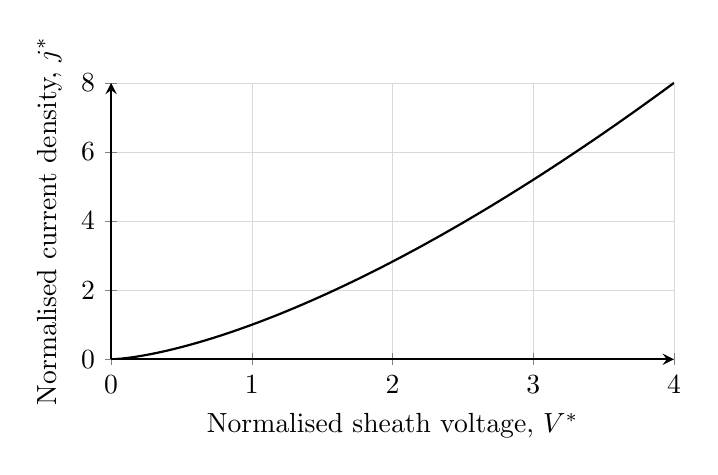
\begin{tikzpicture}
\begin{axis}[
 width=0.72\textwidth,
 height=0.42\textwidth,
 xlabel={Normalised sheath voltage, $V^{*}$},
 ylabel={Normalised current density, $j^{*}$},
 domain=0:4,
 samples=100,
 xmin=0, xmax=4,
 ymin=0, ymax=8,
 axis lines=left,
 grid=both,
 grid style={line width=0.1pt, draw=gray!30},
 thick,
]
\addplot[black, thick] {x^1.5};
\end{axis}
\end{tikzpicture}
\caption{Schematic plot of the analytic Child--Langmuir scaling $j^{*} = \left(V^{*}\right)^{3/2}$ relating normalised current density to normalised sheath voltage. A purely analytic function shown to illustrate the sheath voltage--flux nonlinearity; it does not represent measured, simulated, or fitted data.}
\label{fig:childlaw}
\end{figure}

\subsection{Summary}
\label{ssec:conclusion-summary}

This monograph set out to close a specific gap: the absence of a rigorous, uncertainty-quantified, cross-validated method for combining the partial information supplied by bulk-plasma, sheath-boundary, and surface-response diagnostics into a single trustworthy estimate of the ion energy flux $\Gamma_{E}$ delivered across a plasma sheath. Building on the kinetic definition of $\Gamma_{E}$ (Equation~\ref{eq:conclusion-GammaE-def}), the generalised Bohm criteria fixing the sheath-edge boundary condition \cite{ref0001,ref0013,ref0017}, and a Bayesian multi-diagnostic fusion architecture adapted from integrated-data-analysis practice in magnetic-confinement diagnostics \cite{ref0706,ref0707,ref0709,ref0711,ref0727}, the monograph has assembled a framework that qualifies and reconciles existing sheath diagnostics rather than competing with them, converting individually incomplete measurements into a single, traceable, credible-interval-bearing estimate. Cross-validated against surface-response observables \cite{ref0093,ref0074,ref0075,ref0105} and left open to data-driven closure refinement \cite{ref0101} and surrogate-accelerated real-time deployment \cite{ref0728,ref0731}, the framework is offered as a way of making the existing diagnostic base collectively more useful and actionable than the sum of its individually reported parts.


\appendix
\part{Appendices}
\chapter{Physical Constants, Units, and Notation}
\label{app:notation}

This appendix collects the physical constants, unit conventions, and notational
choices used throughout the monograph. It complements the Nomenclature in the
front matter.

\section{Physical constants}
\begin{longtable}{@{}p{6.8cm}p{2.8cm}p{4.4cm}@{}}
\toprule
\textbf{Constant} & \textbf{Symbol} & \textbf{Value (SI)} \\
\midrule
\endhead
Elementary charge & $e$ & \SI{1.602176634e-19}{\coulomb} \\
Electron mass & $m_{\mathrm{e}}$ & \SI{9.1093837015e-31}{\kilogram} \\
Proton mass & $m_{\mathrm{p}}$ & \SI{1.67262192369e-27}{\kilogram} \\
Boltzmann constant & $k_{\mathrm{B}}$ & \SI{1.380649e-23}{\joule\per\kelvin} \\
Vacuum permittivity & $\varepsilon_{0}$ & \SI{8.8541878128e-12}{\farad\per\metre} \\
Speed of light & $c$ & \SI{2.99792458e8}{\metre\per\second} \\
Planck constant & $h$ & \SI{6.62607015e-34}{\joule\second} \\
Atomic mass unit & $u$ & \SI{1.66053906660e-27}{\kilogram} \\
Avogadro constant & $N_{\mathrm{A}}$ & \SI{6.02214076e23}{\per\mole} \\
\bottomrule
\end{longtable}

\section{Unit conventions}
Plasma temperatures are expressed as energies in electronvolts
(\SI{1}{\electronvolt} $\leftrightarrow$ \SI{11604}{\kelvin} to four significant
figures). Number densities are quoted in \si{\per\cubic\metre}; where the
low-temperature-plasma literature is followed, values may also appear in
\si{\per\cubic\centi\metre} (\SI{1}{\per\cubic\centi\metre} $=$
\SI{1e6}{\per\cubic\metre}). Energy fluxes are given in \si{\watt\per\square\metre}
and particle fluxes in \si{\per\square\metre\per\second}. Pressures follow the SI
pascal, with the equivalence \SI{1}{\pascal} $\approx$ \SI{7.5}{mTorr} noted where
processing pressures are discussed.

\section{Frequently used relations}
\begin{longtable}{@{}p{5.2cm}p{9.2cm}@{}}
\toprule
\textbf{Quantity} & \textbf{Expression} \\
\midrule
\endhead
Debye length & $\lambda_{\mathrm{D}} = \sqrt{\varepsilon_{0} k_{\mathrm{B}} T_{\mathrm{e}} / (n_{\mathrm{e}} e^{2})}$ \\
Electron plasma frequency & $\omega_{\mathrm{pe}} = \sqrt{n_{\mathrm{e}} e^{2} / (\varepsilon_{0} m_{\mathrm{e}})}$ \\
Bohm velocity & $u_{\mathrm{B}} = \sqrt{k_{\mathrm{B}} T_{\mathrm{e}} / m_{\mathrm{i}}}$ \\
Ion (Bohm) flux & $\Gamma_{\mathrm{i}} = n_{\mathrm{s}} u_{\mathrm{B}}$ \\
Floating-sheath potential drop & $\Delta\phi \approx \dfrac{k_{\mathrm{B}} T_{\mathrm{e}}}{2e}\,\ln\!\left(\dfrac{m_{\mathrm{i}}}{2\pi m_{\mathrm{e}}}\right)$ \\
Ion energy flux & $\Gamma_{E} = \displaystyle\int \tfrac{1}{2} m_{\mathrm{i}} v^{2}\, v\, f_{\mathrm{i}}(v)\, \mathrm{d}v$ \\
\bottomrule
\end{longtable}

\section{Notational conventions}
Vectors are set in bold ($\bm{E}$, $\bm{v}$); scalars in italic. Subscripts
$\mathrm{e}$ and $\mathrm{i}$ denote electron and ion quantities; a subscript
$\mathrm{s}$ denotes evaluation at the sheath edge; a subscript $\mathrm{w}$
denotes the wall. The symbol $f_{\mathrm{i}}(\bm{v})$ denotes the ion velocity
distribution function; angle brackets $\langle\cdot\rangle$ denote a
velocity-space average. Reconstructed (inverted) quantities carry a hat, e.g.
$\hat{\Gamma}_{E}$, to distinguish them from the underlying true value
$\Gamma_{E}$.

\chapter{Reference Diagnostic Specifications}
\label{app:specs}

This appendix collects representative instrument specifications for the four optical diagnostic families used in the monograph -- optical emission spectroscopy (OES), laser-induced fluorescence (LIF), Thomson scattering, and interferometry -- and states the optical-access constraints a sheath-edge ion-energy-flux campaign must satisfy. The values are \emph{representative}, compiled from the literature rather than measured by the present authors, and characterise no specific instrument; they bound how precisely $T_{\mathrm{e}}$, $T_{\mathrm{i}}$, $n_{\mathrm{e}}$, $n_{\mathrm{i}}$, $\lambda_{\mathrm{D}}$, $u_{\mathrm{B}}$, and ultimately $\Gamma_{E}$ and $f_{\mathrm{i}}(v)$, can be inferred optically.

\section{Purpose and Scope of Reference Specifications}
\label{sec:specs-scope}

The main text expresses ion energy flux delivered to a plasma-facing surface as a functional of $f_{\mathrm{i}}(v)$ at the sheath edge,
\begin{equation}
\Gamma_{E} = \int_{0}^{\infty} \tfrac{1}{2} M v^{2} \, v \, f_{\mathrm{i}}(v) \, \mathrm{d}v ,
\label{eq:specs-gammaE}
\end{equation}
where $M$ is the ion mass and $f_{\mathrm{i}}(v)$ is normalised to $n_{\mathrm{i}}$. Each diagnostic supplies a partial window onto Eq.~\eqref{eq:specs-gammaE}: OES and Thomson scattering give $T_{\mathrm{e}}$ and $n_{\mathrm{e}}$, setting the Bohm speed
\begin{equation}
u_{\mathrm{B}} = \sqrt{\frac{k_{\mathrm{B}} T_{\mathrm{e}}}{M}} ,
\label{eq:specs-bohm}
\end{equation}
LIF resolves $f_{\mathrm{i}}(v)$ directly, and interferometry gives an independent, line-integrated $n_{\mathrm{e}}$ for cross-calibration. No single technique closes Eq.~\eqref{eq:specs-gammaE}; a credible determination combines at least two diagnostics sharing a calibration and a measurement volume referenced to the Debye length
\begin{equation}
\lambda_{\mathrm{D}} = \sqrt{\frac{\varepsilon_{0} k_{\mathrm{B}} T_{\mathrm{e}}}{n_{\mathrm{e}} e^{2}}} .
\label{eq:specs-debye}
\end{equation}

\section{Optical Emission Spectroscopy}
\label{sec:specs-oes}

OES is the least invasive, least expensive of the four, needing only a single collection optic and no probe beam. It returns line-integrated rather than localised information unless combined with Abel inversion, and its $T_{\mathrm{e}}$/$n_{\mathrm{e}}$ inference depends on a CR model rather than a first-principles relation \cite{ref0231,ref0237}.

\subsection{Spectrometer and Detector Architecture}

Representative OES systems use a Czerny--Turner spectrograph coupled to the plasma via a fibre bundle with $\mathrm{NA} \approx 0.1$--$0.22$. Angular dispersion follows the grating equation,
\begin{equation}
m \lambda = d \left( \sin\theta_{i} + \sin\theta_{d} \right) ,
\label{eq:specs-grating}
\end{equation}
with $m$ the diffraction order, $d$ the groove spacing, $\theta_{i}$, $\theta_{d}$ the incidence/diffraction angles. Differentiating at fixed $\theta_{i}$ and combining with focal length $f$ gives the reciprocal linear dispersion,
\begin{equation}
\mathcal{R} \equiv \frac{\mathrm{d}\lambda}{\mathrm{d}x} \approx \frac{d \cos\theta_{d}}{m f} ,
\label{eq:specs-dispersion}
\end{equation}
typically $\sim\SI{1}{\nano\meter\per\milli\meter}$ for a $\SI{0.5}{\meter}$ instrument with an $\SI{1800}{grooves\per\milli\meter}$ grating, though slit width and pixel sampling set the practical instrument function.

Detection uses a back-illuminated CCD/sCMOS for survey work, a gated ICCD/PMT for fast transients such as sheath formation \cite{ref0256}, or a photon-counting PMT for photometric accuracy.

\subsection{Line Selection and Collisional-Radiative Inference}

Since OES does not measure a velocity distribution, $T_{\mathrm{e}}$ and $n_{\mathrm{e}}$ are inferred from line intensities via a CR model balancing electron-impact excitation, radiative decay, and de-excitation \cite{ref0237,ref0245}. For a thin, steady-state level $p$, transition $p \to q$ intensity scales as
\begin{equation}
I_{pq} \; \propto \; n_{\mathrm{e}} \, n_{0} \, \langle \sigma_{pq}^{\mathrm{exc}} v_{\mathrm{e}} \rangle \, A_{pq} \Big/ \sum_{r<p} A_{pr} ,
\label{eq:specs-crmodel}
\end{equation}
where $n_{0}$ is the ground-state density, $\langle \sigma_{pq}^{\mathrm{exc}} v_{\mathrm{e}} \rangle$ the Maxwellian-averaged excitation rate coefficient, and $A_{pq}$ the spontaneous emission coefficient. The ratio of two lines with different upper-level energies cancels $n_{\mathrm{e}} n_{0}$, giving a ratio monotonic in $T_{\mathrm{e}}$ alone and invertible against a CR grid; a second line pair then returns $n_{\mathrm{e}}$ \cite{ref0231}.

\subsection{Representative OES Specification Table}

\begin{table}[htbp]
\centering
\caption{Representative (illustrative, non-measured) optical emission spectroscopy specifications.}
\label{tab:oes-specs}
\begin{tabular}{@{}ll@{}}
\toprule
Parameter & Representative value \\
\midrule
Spectrometer architecture & Czerny--Turner / crossed Czerny--Turner \\
Focal length & \SI{0.3}{\meter} -- \SI{1.0}{\meter} \\
Grating groove density & \SIrange{300}{2400}{grooves\per\milli\meter} \\
Spectral coverage & \SIrange{200}{1000}{\nano\meter} \\
Spectral resolution (FWHM) & \SIrange{0.02}{0.15}{\nano\meter} \\
Entrance-slit width & \SIrange{10}{100}{\micro\meter} \\
Collection optic & Fibre bundle, $\mathrm{NA} \approx 0.10$--$0.22$ \\
Detector & Back-illuminated CCD / sCMOS / ICCD / PMT \\
Quantum efficiency (peak) & \SIrange{40}{95}{\percent} \\
Dynamic range & $10^{3}$--$10^{5}$ (16-bit typical) \\
Minimum gate width (ICCD) & \SIrange{2}{5}{\nano\second} \\
Typical integration time & \SIrange{1}{1000}{\milli\second} \\
Spatial resolution along l.o.s. & \SIrange{1}{5}{\milli\meter} (fibre-limited) \\
\bottomrule
\end{tabular}
\end{table}

\section{Laser-Induced Fluorescence}
\label{sec:specs-lif}

LIF most directly targets $f_{\mathrm{i}}(v)$: a narrow-linewidth, frequency-scanned laser is tuned across an ionic (or, for two-photon LIF, atomic) transition, and fluorescence intensity vs.\ frequency reproduces the Doppler-broadened absorption profile, proportional to the projection of $f_{\mathrm{i}}(v)$ along the laser $k$-vector \cite{ref0292,ref0300}. Spatially localised and needing no equilibrium assumption, it suits non-Maxwellian, sheath-accelerated ions \cite{ref0304,ref0322}.

\subsection{Laser Source and Tuning}

Representative LIF systems for singly ionised noble gases (e.g.\ ArII near $\SI{670}{\nano\meter}$) use external-cavity/distributed-feedback diode lasers, or CW ring dye/Ti:sapphire lasers outside the diode band, with mode-hop-free tuning over $\SIrange{10}{60}{\giga\hertz}$ and linewidth below the Doppler width. The Doppler FWHM for an ion of mass $M$ at temperature $T_{\mathrm{i}}$ is
\begin{equation}
\Delta\nu_{\mathrm{D}} = \frac{\nu_{0}}{c} \sqrt{\frac{8 \ln 2 \, k_{\mathrm{B}} T_{\mathrm{i}}}{M}} ,
\label{eq:specs-doppler}
\end{equation}
giving $\Delta\nu_{\mathrm{D}} \sim \SI{3}{\giga\hertz}$ for Ar$^{+}$ at $T_{\mathrm{i}} \sim \SI{0.3}{\electronvolt}$, resolved by a $\lesssim \SI{10}{\mega\hertz}$ laser. Irradiance must stay below saturation ($\sim\SI{1}{\milli\watt\per\milli\meter\squared}$) to avoid power broadening.

\subsection{Excitation Scheme and Detection}

The pump beam is chopped at a few kHz to tens of kHz, and fluorescence is demodulated with a lock-in amplifier or gated photon counter, suppressing unmodulated self-emission \cite{ref0300,ref0304}. The fluorescence photon, on a decay branch distinct from the pump wavelength, is detected by a PMT or avalanche photodiode behind an interference filter. TALIF, needed for ground-state species, uses pulsed, frequency-multiplied sources with extra Rabi/photoionisation-loss constraints. Spatial resolution is set by the pump-beam waist (typically $\SIrange{0.2}{1}{\milli\meter}$) and the collection field of view, usually at $\SI{90}{\degree}$ to minimise scattered light.

\subsection{Representative LIF Specification Table}

\begin{table}[htbp]
\centering
\caption{Representative (illustrative, non-measured) laser-induced fluorescence specifications.}
\label{tab:lif-specs}
\begin{tabular}{@{}ll@{}}
\toprule
Parameter & Representative value \\
\midrule
Laser type & External-cavity / distributed-feedback diode, or CW ring dye \\
Tuning range (mode-hop-free) & \SIrange{10}{60}{\giga\hertz} \\
Intrinsic laser linewidth & \SIrange{1}{10}{\mega\hertz} \\
Typical pump wavelength & \SIrange{375}{800}{\nano\meter} (species-dependent) \\
Output power (CW single-photon LIF) & \SIrange{10}{200}{\milli\watt} \\
Pulse energy (TALIF, pulsed) & \SIrange{0.1}{5}{\milli\joule} per pulse \\
Beam waist at focus & \SIrange{0.2}{1.0}{\milli\meter} \\
Modulation / chop frequency & \SIrange{1}{50}{\kilo\hertz} \\
Detector & PMT or avalanche photodiode \\
Spectral discrimination & Interference filter, $\Delta\lambda \sim \SIrange{1}{10}{\nano\meter}$ \\
Signal recovery & Lock-in amplifier / gated photon counting \\
Achievable velocity resolution & $\lesssim \SI{100}{\meter\per\second}$ \\
Spatial resolution & \SIrange{0.2}{2}{\milli\meter} \\
\bottomrule
\end{tabular}
\end{table}

\section{Thomson Scattering}
\label{sec:specs-thomson}

Thomson scattering alone provides $T_{\mathrm{e}}$ and $n_{\mathrm{e}}$ from a first-principles cross section, independent of any atomic model or branching ratios \cite{ref0354,ref0384}. Its cost is the tiny differential cross section of free-electron scattering,
\begin{equation}
\frac{\mathrm{d}\sigma_{\mathrm{T}}}{\mathrm{d}\Omega} = r_{\mathrm{e}}^{2} \sin^{2}\chi , \qquad \sigma_{\mathrm{T}} = \frac{8\pi}{3} r_{\mathrm{e}}^{2} \approx \SI{6.652e-29}{\meter\squared} ,
\label{eq:specs-thomson-xsec}
\end{equation}
where $r_{\mathrm{e}} = e^{2}/(4\pi\varepsilon_{0} m_{\mathrm{e}} c^{2}) \approx \SI{2.818e-15}{\meter}$ is the classical electron radius and $\chi$ the polarisation-observation angle. Eight orders of magnitude smaller than Rayleigh cross sections, it demands a high-energy probe laser, low-stray-light optics, and absolute Raman/Rayleigh calibration in a reference gas \cite{ref0357,ref0362}.

\subsection{Scattering Geometry and Cross Section}

The scattering wavevector $\vec{k} = \vec{k}_{\mathrm{s}} - \vec{k}_{\mathrm{i}}$ has magnitude $k = (4\pi/\lambda_{0}) \sin(\theta/2)$, and the dimensionless parameter
\begin{equation}
\alpha \equiv \frac{1}{k \lambda_{\mathrm{D}}}
\label{eq:specs-alpha}
\end{equation}
sets the regime: for $\alpha \ll 1$ (non-collective) the spectrum reproduces the electron velocity distribution along $\vec{k}$, with Doppler width
\begin{equation}
\Delta\lambda_{1/e} \approx \frac{2\lambda_{0}}{c} \sin\!\left(\frac{\theta}{2}\right) \sqrt{\frac{2 k_{\mathrm{B}} T_{\mathrm{e}}}{m_{\mathrm{e}}}} ,
\label{eq:specs-thomson-doppler}
\end{equation}
from which $T_{\mathrm{e}}$ follows by spectral fit and $n_{\mathrm{e}}$ from the absolute scattered power once calibrated. For $\alpha \gtrsim 1$ (collective), satellites encode $n_{\mathrm{e}}$, $T_{\mathrm{e}}$, $T_{\mathrm{i}}$ jointly; values below assume non-collective scattering.

\subsection{Laser and Collection Optics}

Representative systems use a pulsed, frequency-doubled Nd:YAG laser at $\SI{532}{\nano\meter}$ (or $\SI{1064}{\nano\meter}$) delivering $\SIrange{100}{1000}{\milli\joule}$ in $\SIrange{5}{10}{\nano\second}$ pulses, focused to a few-hundred-micrometre waist \cite{ref0357}. Collection optics sit at $\SI{90}{\degree}$ to the laser to minimise stray light, imaged onto a triple-grating or subtractive-dispersion spectrometer for rejection at the laser wavelength, since the Doppler-shifted signal lies within a few nanometres of it in cold plasmas. Detection is a gated ICCD synchronised to the pulse with nanosecond jitter, rejecting self-emission \cite{ref0362}.

\subsection{Representative Thomson Scattering Specification Table}

\begin{table}[htbp]
\centering
\caption{Representative (illustrative, non-measured) Thomson scattering diagnostic specifications.}
\label{tab:thomson-specs}
\begin{tabular}{@{}ll@{}}
\toprule
Parameter & Representative value \\
\midrule
Laser & Pulsed Nd:YAG, \SI{532}{\nano\meter} (2$\omega$) or \SI{1064}{\nano\meter} \\
Pulse energy & \SIrange{100}{1000}{\milli\joule} \\
Pulse duration & \SIrange{5}{10}{\nano\second} \\
Repetition rate & \SIrange{10}{30}{\hertz} (up to \SI{20}{\kilo\hertz} for burst systems) \\
Focal spot diameter & \SIrange{100}{500}{\micro\meter} \\
Scattering angle & \SI{90}{\degree} (typical) \\
Collection $f$-number & $f/4$ -- $f/10$ \\
Spectrometer & Triple-grating / subtractive-dispersion, stray-light rejection $\gtrsim 10^{-13}$ \\
Detector & Gated ICCD, gate width \SIrange{5}{20}{\nano\second} \\
Absolute calibration method & Rotational Raman or Rayleigh scattering in reference gas \\
Accessible $T_{\mathrm{e}}$ range & \SIrange{0.1}{100}{\electronvolt} \\
Accessible $n_{\mathrm{e}}$ range & $10^{17}$ -- $10^{21}\ \si{\per\meter\cubed}$ \\
Spatial resolution & \SIrange{0.1}{1}{\milli\meter} (laser-waist limited) \\
\bottomrule
\end{tabular}
\end{table}

\section{Interferometry}
\label{sec:specs-interferometry}

Interferometry measures the plasma's contribution to refractive index along a probe chord, unique among the four in needing no photometric calibration or atomic model: the observable is a phase shift, with uncertainty set by mechanical/vibrational stability rather than cross sections \cite{ref0391}. Its limitation is that this observable is a line integral of $n_{\mathrm{e}}$, requiring multi-chord tomography or an assumed symmetry for spatial resolution.

\subsection{Phase-Shift Principle}

For a probe wave of angular frequency $\omega$ through an unmagnetised plasma of density $n_{\mathrm{e}}(\vec{r})$, the refractive index is
\begin{equation}
\eta(\vec{r}) = \sqrt{1 - \frac{\omega_{\mathrm{pe}}^{2}(\vec{r})}{\omega^{2}}} \approx 1 - \frac{n_{\mathrm{e}}(\vec{r})}{2 n_{\mathrm{c}}} , \qquad n_{\mathrm{c}} = \frac{\varepsilon_{0} m_{\mathrm{e}} \omega^{2}}{e^{2}} ,
\label{eq:specs-refractive-index}
\end{equation}
valid for $n_{\mathrm{e}} \ll n_{\mathrm{c}}$, the critical density. Comparing the phase along a chord of length $L$ against a vacuum reference gives
\begin{equation}
\Delta\varphi = \frac{2\pi}{\lambda} \int_{0}^{L} \bigl[1 - \eta(\vec{r})\bigr] \, \mathrm{d}\ell \; \approx \; \frac{e^{2}\lambda}{4\pi \varepsilon_{0} m_{\mathrm{e}} c^{2}} \int_{0}^{L} n_{\mathrm{e}} \, \mathrm{d}\ell \; = \; r_{\mathrm{e}} \lambda \int_{0}^{L} n_{\mathrm{e}} \, \mathrm{d}\ell ,
\label{eq:specs-phase-shift}
\end{equation}
i.e.\ the phase shift is proportional to the line-integrated density and to $\lambda$. Long-wavelength (far-infrared/THz/microwave) interferometers thus suit low-density plasmas, while visible-wavelength interferometry suits denser laser-produced or pulsed-power plasmas \cite{ref0400}.

\subsection{Configurations}

Representative configurations include two-beam Mach--Zehnder/Michelson layouts, recombining a probe beam with an unperturbed reference, and heterodyne (dispersion) interferometers, converting a small frequency offset into a beat-frequency measurement insensitive to vibration \cite{ref0400}. Multi-chord systems permit tomographic (Abel) inversion to a radially resolved $n_{\mathrm{e}}(r)$; single-chord systems return only path-integrated density, commonly cross-validated against Thomson scattering \cite{ref0391}.

\subsection{Representative Interferometry Specification Table}

\begin{table}[htbp]
\centering
\caption{Representative (illustrative, non-measured) interferometry diagnostic specifications.}
\label{tab:interferometry-specs}
\begin{tabular}{@{}ll@{}}
\toprule
Parameter & Representative value \\
\midrule
Configuration & Mach--Zehnder / Michelson / heterodyne (dispersion) \\
Probe wavelength & \SI{632.8}{\nano\meter} (HeNe) to \SI{10.6}{\micro\meter} (CO$_2$), or mm-wave/THz \\
Number of chords & 1 (single-chord) to $\sim$16 (tomographic) \\
Phase resolution & $2\pi/100$ -- $2\pi/1000$ rad \\
Minimum detectable line-integrated $n_{\mathrm{e}}$ & $10^{16}$ -- $10^{18}\ \si{\per\meter\squared}$ \\
Time resolution & \SIrange{0.1}{10}{\micro\second} \\
Detector & Photodiode / pyroelectric / Schottky mixer (frequency-dependent) \\
Path-length stability requirement & $\ll \lambda/10$ over acquisition window \\
Spatial resolution (tomographic) & \SIrange{1}{10}{\milli\meter} (inversion-limited) \\
\bottomrule
\end{tabular}
\end{table}

\section{Optical Access and Integration Requirements}
\label{sec:specs-integration}

Deploying two or more diagnostics on one test article to close Eq.~\eqref{eq:specs-gammaE} imposes mechanical, optical, and timing constraints beyond any single instrument.

\subsection{Viewport and Standoff Constraints}

Every diagnostic volume must sit far enough from the plasma-facing surface to sample the quasi-neutral bulk or presheath, rather than the space-charge sheath whose thickness $s$ collapses toward the wall on the scale of $\lambda_{\mathrm{D}}$. For a planar, collisionless sheath, Child-law scaling gives normalised thickness vs.\ potential drop $\eta \equiv eV_{0}/(k_{\mathrm{B}} T_{\mathrm{e}})$,
\begin{equation}
\frac{s}{\lambda_{\mathrm{D}}} \; \approx \; \frac{\sqrt{2}}{3} \, (2\eta)^{3/4} ,
\label{eq:specs-childlaw}
\end{equation}
which grows only as $\eta^{3/4}$ but reaches several tens of Debye lengths for $\eta \sim 10^{2}$--$10^{3}$, typical of RF-biased surfaces (Fig.~\ref{fig:childlaw-sheath}), motivating the standoff distances in Table~\ref{tab:integration-specs}.

\begin{figure}[htbp]
\centering
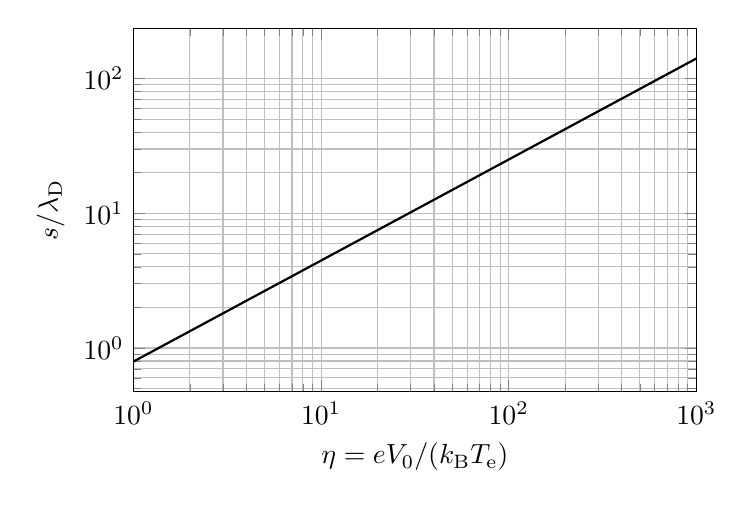
\begin{tikzpicture}
\begin{axis}[
 width=0.72\textwidth,
 height=6.2cm,
 xmode=log, ymode=log,
 xlabel={$\eta = eV_{0}/(k_{\mathrm{B}} T_{\mathrm{e}})$},
 ylabel={$s/\lambda_{\mathrm{D}}$},
 grid=both,
 domain=1:1000,
 samples=120,
 xmin=1, xmax=1000,
 axis lines=box,
]
\addplot[thick, black] {(sqrt(2)/3)*(2*x)^(0.75)};
\end{axis}
\end{tikzpicture}
\caption{Analytic Child-law scaling of the collisionless planar sheath thickness $s/\lambda_{\mathrm{D}}$ (Eq.~\eqref{eq:specs-childlaw}); motivates the standoff distances in Table~\ref{tab:integration-specs}. Not measured data.}
\label{fig:childlaw-sheath}
\end{figure}

Measurement volumes should sit at least several sheath thicknesses -- typically $\SIrange{1}{10}{\milli\meter}$ here -- from the wall, so the sampled population is unperturbed presheath or bulk plasma. Figure~\ref{fig:optical-access-schematic} sketches how the four beams can be arranged around a common volume at this standoff.

\begin{figure}[htbp]
\centering
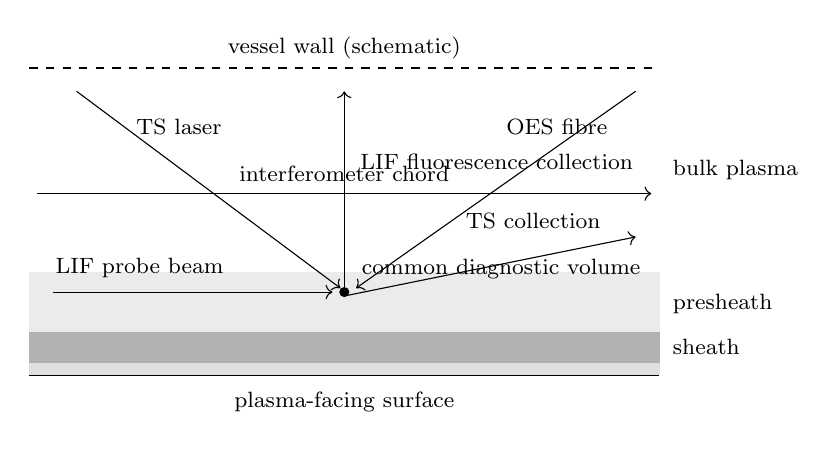
\begin{tikzpicture}[scale=1.0, every node/.style={font=\footnotesize}]
 \draw[very thick] (-4,0) -- (4,0);
 \filldraw[black!12] (-4,0) rectangle (4,0.15);
 \node at (0,-0.35) {plasma-facing surface};
 \filldraw[black!30] (-4,0.15) rectangle (4,0.55);
 \node[anchor=west] at (4.05,0.35) {sheath};
 \filldraw[black!8] (-4,0.55) rectangle (4,1.3);
 \node[anchor=west] at (4.05,0.9) {presheath};
 \node[anchor=west] at (4.05,2.6) {bulk plasma};
 \filldraw[black] (0,1.05) circle (1.6pt);
 \node[anchor=south west] at (0.1,1.1) {common diagnostic volume};
 \draw[->] (3.7,3.6) -- (0.15,1.1);
 \node at (2.7,3.15) {OES fibre};
 \draw[->] (-3.7,1.05) -- (-0.15,1.05);
 \node at (-2.6,1.35) {LIF probe beam};
 \draw[->] (0,1.05) -- (0,3.6);
 \node[anchor=west] at (0.08,2.7) {LIF fluorescence collection};
 \draw[->] (-3.4,3.6) -- (-0.05,1.1);
 \node at (-2.1,3.15) {TS laser};
 \draw[->] (0,1.0) -- (3.7,1.75);
 \node at (2.4,1.95) {TS collection};
 \draw[->] (-3.9,2.3) -- (3.9,2.3);
 \node at (0,2.55) {interferometer chord};
 \draw[thick, dashed] (-4,3.9) -- (4,3.9);
 \node at (0,4.15) {vessel wall (schematic)};
\end{tikzpicture}
\caption{Schematic (not to scale) optical access for the four diagnostics about a common measurement volume beyond the sheath, in the presheath/bulk plasma. Indicative only.}
\label{fig:optical-access-schematic}
\end{figure}

Windows must transmit every wavelength in simultaneous use (materials in Table~\ref{tab:integration-specs}); in sputtering environments a shutter, gas curtain, or sacrificial flat should protect them from film buildup.

\subsection{Synchronization and Multi-Diagnostic Integration}

Operating pulsed diagnostics (Thomson scattering, pulsed LIF/TALIF) alongside continuous ones (OES, CW LIF, interferometry) requires a common timing reference with jitter well below the shortest timescale of interest -- typically the RF period or ion-transit time across the sheath. A representative budget (Table~\ref{tab:integration-specs}) ranges from $\lesssim \SI{1}{\nano\second}$, synchronising the Thomson laser Q-switch to the ICCD gate, to $\lesssim \SI{1}{\micro\second}$ for aligning OES/interferometer acquisition. Cross-calibration matters equally: absolute density from Thomson scattering and line-integrated density from interferometry (Eq.~\eqref{eq:specs-phase-shift}) give two independent routes to $n_{\mathrm{e}}$, checked for agreement before combining OES-inferred $T_{\mathrm{e}}$ with LIF-inferred $f_{\mathrm{i}}(v)$ in Eq.~\eqref{eq:specs-gammaE}.

\subsection{Representative Integration Requirements Table}

\begin{table}[htbp]
\centering
\caption{Representative (illustrative, non-measured) optical-access and integration requirements.}
\label{tab:integration-specs}
\begin{tabular}{@{}ll@{}}
\toprule
Requirement & Representative value \\
\midrule
Minimum diagnostic-volume standoff from wall & \SIrange{1}{10}{\milli\meter} ($\gtrsim$ several $\lambda_{\mathrm{D}}$--$s$) \\
Window material (visible/UV instruments) & Fused silica / UV-grade sapphire \\
Window material (IR/THz interferometry) & ZnSe / crystal quartz / polyethylene \\
Anti-reflection coating requirement & $R < \SI{0.5}{\percent}$ per surface at operating $\lambda$ \\
Viewport count (minimum, 4-diagnostic system) & 6--8 (probe + collection per instrument) \\
Cross-trigger timing jitter (pulsed instruments) & $\lesssim \SI{1}{\nano\second}$--\SI{10}{\nano\second} \\
Cross-trigger timing jitter (CW/slow instruments) & $\lesssim \SI{1}{\micro\second}$ \\
Mechanical vibration tolerance (interferometry) & $\ll \lambda_{\mathrm{probe}}/10$ path-length change \\
Density cross-check tolerance (Thomson vs.\ interferometry) & Agreement within combined $1\sigma$ uncertainty \\
Window contamination mitigation & Shutter / gas curtain / sacrificial flat \\
\bottomrule
\end{tabular}
\end{table}

\section{Summary}
\label{sec:specs-summary}

This appendix has assembled representative specifications for the four diagnostics providing the observational basis for the sheath-edge quantities entering $\Gamma_{E}$. OES offers the least invasive, least costly route to $T_{\mathrm{e}}$ and $n_{\mathrm{e}}$ but depends on a CR model; LIF alone resolves $f_{\mathrm{i}}(v)$ directly, at the cost of a narrow-linewidth, transition-matched laser; Thomson scattering returns $T_{\mathrm{e}}$ and $n_{\mathrm{e}}$ independent of atomic structure, at the cost of a weak signal needing a high-energy laser and stray-light-optimised collection; and interferometry supplies an independently calibrated, line-integrated density as cross-check. None of the values in Tables~\ref{tab:oes-specs}--\ref{tab:integration-specs}, nor the curves in Figs.~\ref{fig:childlaw-sheath} and \ref{fig:optical-access-schematic}, are measured data; they size the infrastructure for a coherent campaign.

\chapter{Reference Data Tables}
\label{app:data}

This appendix collects the numerical scales used throughout the monograph: ranges of $n_{\mathrm{e}}$, $n_{\mathrm{i}}$, $T_{\mathrm{e}}$, and $T_{\mathrm{i}}$ for the three application domains; sputter-yield thresholds; ion-energy and sheath-potential scales; and reference Debye lengths $\lambda_{\mathrm{D}}$ and Bohm velocities $u_{\mathrm{B}}$ for common gases. Entries are closed-form evaluations of expressions derived in Chapters~2--4, or literature-compiled figures labelled as such; none is an original measurement.

\section{Typical Plasma Parameter Ranges for the Three Application Domains}
\label{app:data:domains}

The main text motivates the ion-energy-flux formalism with three domains sharing the same sheath physics but occupying very different parameter regions: low-temperature RF processing, the magnetically confined fusion boundary (scrape-off layer and divertor), and electric propulsion. Table~\ref{tab:domains} summarises characteristic density, temperatures, magnetic field, pressure, and species for each; values are orientation, not strict bounds.

\begin{table}[htbp]
\centering
\caption{Representative operating ranges of key plasma parameters in the three application domains treated in this monograph. Values are order-of-magnitude, literature-representative ranges, not measurements from this work.}
\label{tab:domains}
\begin{tabularx}{\textwidth}{@{}l X X X@{}}
\toprule
Parameter & RF processing plasma & Fusion edge / divertor & Electric propulsion \\
\midrule
$n_{\mathrm{e}}$ & \SI{1e15}{} -- \SI{1e18}{\per\cubic\meter} & \SI{1e18}{} -- \SI{1e21}{\per\cubic\meter} & \SI{1e15}{} -- \SI{1e19}{\per\cubic\meter} \\
$T_{\mathrm{e}}$ & \SI{1}{} -- \SI{7}{\eV} & \SI{1}{} -- \SI{100}{\eV} & \SI{1}{} -- \SI{30}{\eV} \\
$T_{\mathrm{i}}$ & \SI{0.03}{} -- \SI{0.5}{\eV} & comparable to $T_{\mathrm{e}}$, up to a few $T_{\mathrm{e}}$ & \SI{0.1}{} -- \SI{5}{\eV} (directed beam spread) \\
Magnetic field $B$ & $0$ -- few \si{\milli\tesla} (magnetised ICP) & \SI{1}{} -- \SI{8}{\tesla} & \SI{1}{} -- \SI{20}{\milli\tesla} (radial, Hall channel) \\
Neutral pressure & \SI{0.1}{} -- \SI{13}{\pascal} & effectively vacuum in confined region & \SI{1e-3}{} -- \SI{1}{\pascal} \\
Typical species & Ar, O$_2$, N$_2$, Cl$_2$, SF$_6$ & D, T, He, seeded N/Ne/Ar & Xe, Kr, occasionally I$_2$, Ar \\
\bottomrule
\end{tabularx}
\end{table}

Three features recur. First, $T_{\mathrm{e}}$ stays within a narrow band, $\SI{1}{\eV} \lesssim T_{\mathrm{e}} \lesssim \SI{100}{\eV}$, fixed by the atomic physics of ionisation that sustains a discharge. Second, $n_{\mathrm{e}}$ spans many orders of magnitude, from tenuous thruster plumes to dense divertor plasma, and together with $T_{\mathrm{e}}$ sets the Debye length and sheath thickness (Section~\ref{app:data:debye}). Third, in RF processing and electric-propulsion plasmas $T_{\mathrm{i}} \ll T_{\mathrm{e}}$, an ordering that makes the Bohm criterion tractable \cite{ref0001,ref0013}; in the fusion edge, however, $T_{\mathrm{i}}$ can be comparable to, or a few times, $T_{\mathrm{e}}$, requiring the warm-ion Bohm generalisation discussed in Section~\ref{app:data:energy}.

In the fusion edge, the wide range reflects the transition from the hot upstream SOL to the cold, dense, often detached divertor target \cite{ref0013,ref0017}. In electric propulsion, it reflects the dense, magnetised discharge channel versus the far more tenuous plume; ion energy and flux there underpin erosion and lifetime assessments \cite{ref0074,ref0105}.

\section{Representative Sputter-Yield Thresholds and Trends by Material}
\label{app:data:sputter}

Physical sputtering is the ejection of a surface atom by momentum transferred from an incident ion through a collision cascade, underlying erosion of plasma-facing components, thruster grids, and processing-chamber walls. The key quantity is the sputter yield $Y(E,\theta)$, the mean number of atoms ejected per incident ion of energy $E$ and angle $\theta$. At normal incidence the yield is strongly threshold-like: below $E_{\mathrm{th}}$ the ion cannot overcome the surface binding energy $U_0$ and $Y \to 0$; above threshold $Y$ rises, peaks broadly in the \si{\kilo\eV} range, then falls as the ion penetrates too deeply for the cascade to reach the surface \cite{ref0143,ref0144}.

A widely used empirical parameterisation, due to Bohdansky and refined by Yamamura, writes the yield as a nuclear-stopping cross-section times a threshold factor,
\begin{equation}
Y(E) = Q \, S_{n}(E) \left[1 - \left(\frac{E_{\mathrm{th}}}{E}\right)^{2/3}\right]\left[1 - \frac{E_{\mathrm{th}}}{E}\right]^{2},
\qquad E \geq E_{\mathrm{th}},
\label{appD-eq:bohdansky}
\end{equation}
and $Y(E)=0$ for $E<E_{\mathrm{th}}$, where $Q$ is a material-dependent factor and $S_n(E)$ the reduced nuclear stopping cross-section \cite{ref0144}. The threshold requires the ion to impart energy of order $U_0$ to a target atom in one close collision, giving
\begin{equation}
E_{\mathrm{th}} \approx
\begin{cases}
U_0/[\gamma(1-\gamma)], & M_{\mathrm{i}}/M_{\mathrm{t}} \lesssim 0.3, \\[2pt]
8\,U_0\,(M_{\mathrm{i}}/M_{\mathrm{t}})^{2/5}, & M_{\mathrm{i}}/M_{\mathrm{t}} \gtrsim 0.3,
\end{cases}
\qquad
\gamma = \frac{4 M_{\mathrm{i}} M_{\mathrm{t}}}{(M_{\mathrm{i}}+M_{\mathrm{t}})^{2}},
\label{eq:ethresh}
\end{equation}
with $M_{\mathrm{i}}$, $M_{\mathrm{t}}$ the ion and target masses and $\gamma$ the maximum fractional energy transfer per collision; the first (light-ion) branch applies for mass ratio $M_{\mathrm{i}}/M_{\mathrm{t}} \lesssim 0.3$, the second (near-unity mass ratio) branch otherwise. Light ions (H, D, He) sputter heavy targets (W, Mo) weakly, above a high threshold, since mass mismatch makes $\gamma$ small, while mass-matched pairs (e.g.\ Ar$^+$ on Cu) couple efficiently at low threshold via the second branch.

Table~\ref{tab:sputter} lists representative threshold energies and a reference yield for materials relevant to fusion plasma-facing components and processing. These are order-of-magnitude values: measured yields depend on species, angle, roughness, temperature, and fluence, and can vary by a factor of two between sources \cite{ref0152,ref0158}.

\begin{table}[htbp]
\centering
\caption{Representative (literature-typical) sputter-yield thresholds and reference yields for selected target materials. Values are order-of-magnitude figures compiled from the classical sputtering-yield literature and are \emph{not} measurements from this work; actual yields depend on ion species, angle, surface condition, and fluence.}
\label{tab:sputter}
\begin{tabular}{@{}llccl@{}}
\toprule
Target & Bombarding ion & $E_{\mathrm{th}}$ [\si{\eV}] & $Y$ at \SI{500}{\eV} & Remarks \\
\midrule
W & D$^{+}$ & $\sim 200$--230 & $\sim 10^{-3}$--$10^{-2}$ & high threshold; dominant divertor concern \cite{ref0158} \\
W & He$^{+}$ & $\sim 100$ & $\sim 10^{-2}$--$10^{-1}$ & enhanced by surface nanostructuring \\
W & Ar$^{+}$ & $\sim 30$ & $\sim 0.5$--1 & self-consistent heavy-ion benchmark \\
C (graphite) & D$^{+}$ & $\sim 35$--40 & $\sim 10^{-2}$ (physical only) & chemical erosion dominates below threshold \\
Be & D$^{+}$ & $\sim 10$--15 & $\sim 10^{-2}$--$10^{-1}$ & low threshold; ITER first-wall relevance \\
Mo & Ar$^{+}$ & $\sim 25$ & $\sim 0.7$--1 & alternative divertor material \\
Cu & Ar$^{+}$ & $\sim 17$--20 & $\sim 2$--2.5 & reference material for yield benchmarking \\
Si & Ar$^{+}$ & $\sim 20$ & $\sim 0.5$--0.8 & processing/etch-mask relevance \\
Stainless steel & Ar$^{+}$ & $\sim 20$--25 & $\sim 1$--1.5 & representative of chamber-wall erosion \\
\bottomrule
\end{tabular}
\end{table}

This trend -- light-on-heavy pairs give high threshold and low yield, mass-matched pairs sputter efficiently at low threshold -- follows directly from $\gamma$ in Equation~\eqref{eq:ethresh}, and explains why fusion devices favour D/T fuelling against tungsten walls while accepting more efficient helium-ash erosion \cite{ref0143}. Realistic multi-species bombardment also shows synergistic effects not captured by Equation~\eqref{appD-eq:bohdansky} alone.

Figure~\ref{fig:yield} shows the qualitative shape of Equation~\eqref{appD-eq:bohdansky}, via the bracketed threshold factor
\begin{equation}
\hat{Y}(x) = \left(1-x^{-2/3}\right)\left(1-x^{-1}\right)^{2}, \qquad x \equiv E/E_{\mathrm{th}} \geq 1,
\label{eq:yieldnorm}
\end{equation}
versus reduced energy $x$; it excludes $S_n(E)$ and is not an absolute yield curve for any material.

\begin{figure}[htbp]
\centering
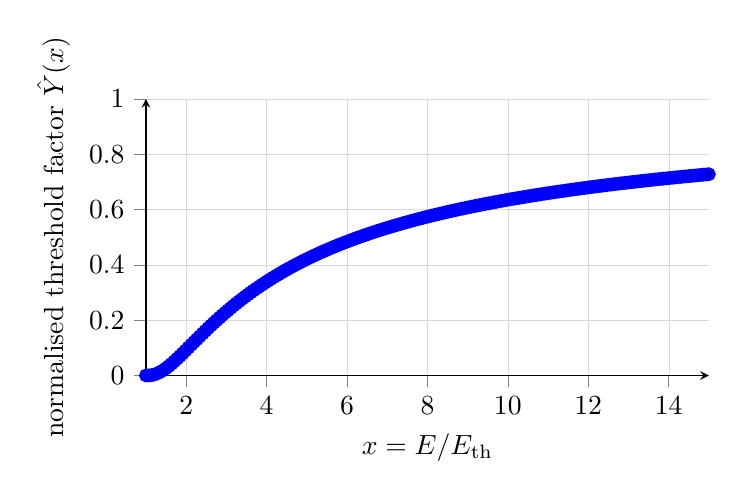
\begin{tikzpicture}
\begin{axis}[
 width=0.72\textwidth,
 height=0.42\textwidth,
 xlabel={$x = E/E_{\mathrm{th}}$},
 ylabel={normalised threshold factor $\hat{Y}(x)$},
 xmin=1, xmax=15,
 ymin=0, ymax=1,
 domain=1:15,
 samples=200,
 axis lines=left,
 tick align=outside,
 grid=major,
 grid style={line width=0.1pt, draw=gray!30},
 every axis plot/.append style={line width=1pt, color=black},
]
\addplot {(1-x^(-2/3))*(1-x^(-1))^2};
\end{axis}
\end{tikzpicture}
\caption{Schematic, dimensionless illustration of the threshold factor $\hat Y(x)$ in the Bohdansky-type sputtering yield model of Equation~\eqref{eq:yieldnorm}, plotted as an explicit analytic function of the reduced energy $x=E/E_{\mathrm{th}}$. This is a mathematical illustration of the model's threshold shape only; it does not represent measured or material-specific yield data.}
\label{fig:yield}
\end{figure}

\section{Ion-Energy and Sheath-Potential Scales}
\label{app:data:energy}

Ion impact energy is set, to leading order, by the potential drop across the sheath, modified by the ion's kinetic energy at the sheath edge (fixed by the Bohm criterion) and, in time-varying sheaths, by transit-time dynamics. This section collects the relations converting a sheath potential into an ion energy flux $\Gamma_E$ at the wall.

\subsection{The Bohm criterion and the presheath potential drop}

A collisionless, quasineutral plasma supports a monotonic potential drop into a sheath only if ions enter the sheath edge at directed speed at or above the Bohm velocity $u_{\mathrm{B}}$,
\begin{equation}
u_{\mathrm{i}}(s) \geq u_{\mathrm{B}} \equiv \sqrt{\frac{k_{\mathrm{B}} T_{\mathrm{e}}}{M}} ,
\label{eq:bohmcrit}
\end{equation}
where $s$ is the sheath edge and $M$ the ion mass; its generalisations (finite $T_{\mathrm{i}}$, collisions, multiple species, magnetisation) form an extensive literature \cite{ref0001,ref0017}. Momentum balance in the presheath, where ions accelerate from bulk thermal speed to $u_{\mathrm{B}}$, requires a drop of order
\begin{equation}
\Delta \phi_{\mathrm{pre}} \sim \frac{1}{2}\,\frac{T_{\mathrm{e}}}{e},
\label{eq:presheath}
\end{equation}
independent, to leading order, of the transport mechanism (collisional friction, geometric divergence, ionisation) \cite{ref0013}. This minimum energy is acquired before the sheath proper, ahead of the typically larger sheath-potential acceleration.

\subsection{The floating potential and the mean bombardment energy}

For a floating, non-emitting surface, zero net current fixes the sheath drop $V_{\mathrm{sh}} = \phi_{\mathrm{s}} - \phi_{\mathrm{w}}$:
\begin{equation}
V_{\mathrm{f}} = \frac{T_{\mathrm{e}}}{2e}\ln\!\left[\frac{M}{2\pi m_{\mathrm{e}}}\right],
\label{eq:floating}
\end{equation}
obtained by equating the Bohm ion flux $n_{\mathrm{s}} u_{\mathrm{B}}$ to the thermal electron flux $\tfrac{1}{4} n_{\mathrm{s}} \bar v_{\mathrm{e}} \exp(-eV_{\mathrm{f}}/T_{\mathrm{e}})$, with $\bar v_{\mathrm{e}} = \sqrt{8 T_{\mathrm{e}}/\pi m_{\mathrm{e}}}$. Since $M/m_{\mathrm{e}}\sim10^{3}$--$10^{5}$, the logarithm is a modest factor, and
\begin{equation}
e V_{\mathrm{f}} \approx (3\text{--}6)\, T_{\mathrm{e}},
\end{equation}
the coefficient depending logarithmically on mass ratio and $T_{\mathrm{i}}/T_{\mathrm{e}}$. On an actively biased surface the drop is set externally, from a few volts to several kilovolts, with ion energy following the instantaneous or time-averaged potential depending on transit time \cite{ref0080,ref0105}.

In the collisionless limit, the mean bombardment energy is
\begin{equation}
\langle E_{\mathrm{i}} \rangle \approx e V_{\mathrm{sh}} + \frac{1}{2}M u_{\mathrm{B}}^{2} + \tfrac{1}{2}T_{\mathrm{i}}
\;=\; e V_{\mathrm{sh}} + \tfrac{1}{2}T_{\mathrm{e}} + \tfrac{1}{2}T_{\mathrm{i}},
\label{eq:meanenergy}
\end{equation}
where the last two terms are minor once bias exceeds a few tens of volts but dominate on an unbiased floating wall. Charge-exchange collisions broaden the distribution about $\langle E_{\mathrm{i}}\rangle$, producing the low-energy tail quantified by $f_{\mathrm{i}}(v)$ below \cite{ref0077}.

\subsection{Ion energy distribution and energy flux}

The ion energy flux to the surface:
\begin{equation}
\Gamma_{E} = \int_{0}^{\infty} \left(\tfrac{1}{2} M v^{2}\right) v\, f_{\mathrm{i}}(v)\, \mathrm{d}v
= \Gamma_{\mathrm{i}} \, \langle E_{\mathrm{i}} \rangle,
\qquad
\Gamma_{\mathrm{i}} = \int_{0}^{\infty} v\, f_{\mathrm{i}}(v)\, \mathrm{d}v = n_{\mathrm{s}} u_{\mathrm{B}},
\label{eq:energyflux}
\end{equation}
where $f_{\mathrm{i}}(v)$ is the wall ion distribution, normalised so $\int_0^\infty f_{\mathrm{i}}(v)\,\mathrm{d}v = n_{\mathrm{s}}$, and $\Gamma_{\mathrm{i}}$ is the particle flux fixed by the Bohm criterion to $n_{\mathrm{s}} u_{\mathrm{B}}$ \cite{ref0074,ref0090,ref0093}. This links to Section~\ref{app:data:sputter}: it is $\Gamma_E$, not $\Gamma_{\mathrm{i}}$ alone, that sets erosion or heat load once folded against a yield $Y(E)$, via $\Gamma_{\mathrm{erosion}} = \int Y(E)\, v\, f_{\mathrm{i}}(v)\, \mathrm{d}v$.

In a time-independent, near-collisionless sheath, $f_{\mathrm{i}}(v)$ collapses toward a narrow distribution centred on Equation~\eqref{eq:meanenergy}. In an RF-driven or pulsed sheath, finite transit time instead broadens $f_{\mathrm{i}}(v)$ into the bimodal or saddle-shaped distribution reported for capacitively coupled discharges \cite{ref0105}. Diagnostics validating Equation~\eqref{eq:energyflux} include secondary-electron, ion-energy, and calorimetric probes \cite{ref0080}.

\subsection{The Child--Langmuir space-charge limit}

At sheath potentials well above $T_{\mathrm{e}}/e$, the sheath becomes space-charge-dominated with negligible electron density inside it, and the ion current is limited by the collisionless, planar Child--Langmuir law:
\begin{equation}
J_{\mathrm{i}} = \frac{4}{9}\,\varepsilon_{0}\sqrt{\frac{2e}{M}}\,\frac{V_{\mathrm{sh}}^{3/2}}{s^{2}},
\label{appD-eq:childlangmuir}
\end{equation}
with $s$ the sheath thickness. Combined with the Bohm flux $J_{\mathrm{i}} = e n_{\mathrm{s}} u_{\mathrm{B}}$, this gives the matrix-sheath / Child-law scaling $s \propto \lambda_{\mathrm{D}} (V_{\mathrm{sh}} / T_{\mathrm{e}})^{3/4}$, the basis for sheath-thickness diagnostics against the Bohm criterion \cite{ref0013,ref0017}.

\section{Debye Length and Bohm Velocity Reference Values for Common Gases}
\label{app:data:debye}

The two scales fixing sheath structure -- the Debye length $\lambda_{\mathrm{D}}$, over which quasineutrality is violated, and the Bohm velocity $u_{\mathrm{B}}$, the minimum ion speed at the sheath edge -- are
\begin{equation}
\lambda_{\mathrm{D}} = \left(\frac{\varepsilon_{0} k_{\mathrm{B}} T_{\mathrm{e}}}{n_{\mathrm{e}} e^{2}}\right)^{1/2},
\qquad
u_{\mathrm{B}} = \left(\frac{k_{\mathrm{B}} T_{\mathrm{e}}}{M}\right)^{1/2}.
\label{eq:debyebohm}
\end{equation}
In practical units ($T_{\mathrm{e}}$ in \si{\eV}, $n_{\mathrm{e}}$ in \si{\per\cubic\meter}, $M$ in \si{\amu}):
\begin{align}
\lambda_{\mathrm{D}}\,[\si{\meter}] &\approx 7.43\times 10^{3}\, \sqrt{\frac{T_{\mathrm{e}}\,[\si{\eV}]}{n_{\mathrm{e}}\,[\si{\per\cubic\meter}]}}, \label{eq:debyenum}\\
u_{\mathrm{B}}\,[\si{\meter\per\second}] &\approx 9.82\times 10^{3}\, \sqrt{\frac{T_{\mathrm{e}}\,[\si{\eV}]}{M\,[\si{\amu}]}}. \label{eq:bohmnum}
\end{align}
$\lambda_{\mathrm{D}}$ depends only on the electron population, independent of ion species; $u_{\mathrm{B}}$ scales as $M^{-1/2}$, so light-ion plasmas strike the wall faster, though not with more energy, since $\tfrac12 M u_{\mathrm{B}}^2 = \tfrac12 T_{\mathrm{e}}$ is independent of $M$.

Table~\ref{tab:gastable} evaluates Equations~\eqref{eq:debyenum}--\eqref{eq:bohmnum} for nine gas species common to the three domains, at a representative $(T_{\mathrm{e}}, n_{\mathrm{e}})$ point each; none are measured.

\begin{longtable}{@{}llcccc@{}}
\caption{Debye length and Bohm velocity reference values for common gas species, evaluated at a representative electron temperature and density typical of the indicated application context. All values are computed from Equations~\eqref{eq:debyenum}--\eqref{eq:bohmnum} and are illustrative reference points, not measured data.}
\label{tab:gastable}\\
\toprule
Species & Representative context & $T_{\mathrm{e}}$ [\si{\eV}] & $n_{\mathrm{e}}$ [\si{\per\cubic\meter}] & $\lambda_{\mathrm{D}}$ & $u_{\mathrm{B}}$ \\
\midrule
\endfirsthead
\multicolumn{6}{c}{\tablename\ \thetable{} -- continued} \\
\toprule
Species & Representative context & $T_{\mathrm{e}}$ [\si{\eV}] & $n_{\mathrm{e}}$ [\si{\per\cubic\meter}] & $\lambda_{\mathrm{D}}$ & $u_{\mathrm{B}}$ \\
\midrule
\endhead
\bottomrule
\endfoot
H ($M=1$) & Fusion edge / SOL & 20 & \SI{3e19}{} & \SI{6.07}{\micro\meter} & \SI{43.9}{\kilo\meter\per\second} \\
D ($M=2$) & Fusion divertor & 10 & \SI{5e19}{} & \SI{3.33}{\micro\meter} & \SI{22.0}{\kilo\meter\per\second} \\
He ($M=4$) & Fusion ash / seeding & 5 & \SI{5e18}{} & \SI{7.43}{\micro\meter} & \SI{11.0}{\kilo\meter\per\second} \\
N ($M=14$) & RF etch (N$_2$ discharge) & 3 & \SI{5e16}{} & \SI{57.6}{\micro\meter} & \SI{4.55}{\kilo\meter\per\second} \\
O ($M=16$) & RF etch (O$_2$ discharge) & 3 & \SI{8e16}{} & \SI{45.5}{\micro\meter} & \SI{4.25}{\kilo\meter\per\second} \\
Ne ($M=20$) & RF sputter deposition & 4 & \SI{1e17}{} & \SI{47.0}{\micro\meter} & \SI{4.39}{\kilo\meter\per\second} \\
Ar ($M=40$) & RF processing benchmark & 3 & \SI{1e17}{} & \SI{40.7}{\micro\meter} & \SI{2.69}{\kilo\meter\per\second} \\
Kr ($M=84$) & Electric propulsion (ion thruster) & 4 & \SI{2e17}{} & \SI{33.3}{\micro\meter} & \SI{2.14}{\kilo\meter\per\second} \\
Xe ($M=131$) & Electric propulsion (Hall thruster) & 20 & \SI{6e17}{} & \SI{42.9}{\micro\meter} & \SI{3.84}{\kilo\meter\per\second} \\
\end{longtable}

Two trends stand out. First, within the fusion-edge rows (H, D, He), $\lambda_{\mathrm{D}}$ stays in the few-\si{\micro\meter} range despite an order-of-magnitude spread in $T_{\mathrm{e}}$, since densities are correspondingly high; the sheath is thus extremely thin compared with the SOL connection length, the basis for treating it as a local boundary condition in edge-transport codes \cite{ref0013}. Second, $u_{\mathrm{B}}$ falls monotonically along H~$\to$~Xe at comparable $T_{\mathrm{e}}$, consistent with $M^{-1/2}$ scaling; this drives the longer ion residence time of heavy species (Xe, Kr) relative to light ones (H, He), relevant to electric-propulsion exhaust analysis \cite{ref0105}.

Away from these points, $\lambda_{\mathrm{D}} \propto \sqrt{T_{\mathrm{e}}/n_{\mathrm{e}}}$: doubling density at fixed temperature shrinks $\lambda_{\mathrm{D}}$, and typically sheath thickness, to $1/\sqrt{2}\approx0.71$ of its value. And $u_{\mathrm{B}} \propto \sqrt{T_{\mathrm{e}}}$ varies only about an order of magnitude over the full $T_{\mathrm{e}}$ range of Table~\ref{tab:domains}, whereas $n_{\mathrm{e}}$ -- and hence $\Gamma_{\mathrm{i}}=n_{\mathrm{s}}u_{\mathrm{B}}$ -- varies by several orders of magnitude; density dominates the dynamic range of ion flux delivered to a surface.

\section{Summary}

This appendix has assembled the reference numbers translating the sheath-theory formalism into concrete operating scales: plasma windows for RF, fusion-edge, and electric-propulsion plasmas (Table~\ref{tab:domains}); sputter-yield thresholds and their origin in the mass-transfer factor of Equation~\eqref{eq:ethresh} (Table~\ref{tab:sputter}, Figure~\ref{fig:yield}); the chain of relations -- Bohm criterion, presheath drop, floating potential, mean bombardment energy, ion energy flux, and the Child--Langmuir limit -- connecting a sheath potential to a surface energy flux $\Gamma_E$ (Equations~\eqref{eq:bohmcrit}--\eqref{appD-eq:childlangmuir}); and Debye-length and Bohm-velocity values for nine gases (Table~\ref{tab:gastable}). Sputtering figures are literature-representative; Debye and Bohm entries are direct evaluations of Equation~\eqref{eq:debyebohm}.

\chapter{Annotated Bibliography of Seminal Works}
\label{app:annot}

The framework developed in this monograph for quantifying ion energy flux across plasma sheaths draws on seven interlocking bodies of literature: kinetic and fluid theory of the sheath and presheath; the definition and measurement of ion energy flux at bounding surfaces; non-perturbative laser-induced-fluorescence (LIF) diagnostics of the ion velocity distribution function (IVDF); Thomson-scattering diagnostics of the electron population adjoining the sheath; the mathematics of ill-posed inverse problems used to reconstruct distribution functions and profiles from noisy data; erosion and lifetime studies in Hall-effect thrusters; and plasma-wall interaction (PWI) in magnetically confined fusion devices. This appendix is not an exhaustive survey; it selects works judged most seminal to the chain of reasoning used in the main text --- from the Bohm criterion, through the definition of the energy-resolved ion flux $\Gamma_{E}$, to its diagnostic reconstruction and consequences for wall erosion. Entries are grouped by theme, each opening with a paragraph fixing notation and the governing equation the theme's works refine. No cited or plotted quantity here should be read as a measurement by the present authors; all figures are schematic. Notation is fixed throughout: $T_{\mathrm{e}}$ and $T_{\mathrm{i}}$ denote electron and ion temperature in energy units, $n_{\mathrm{e}}$ and $n_{\mathrm{i}}$ the corresponding number densities, $\lambda_{\mathrm{D}} = \sqrt{\varepsilon_{0} T_{\mathrm{e}}/n_{\mathrm{e}} e^{2}}$ the electron Debye length, $u_{\mathrm{B}}$ the Bohm speed, $\Gamma_{E}$ the ion energy flux density, and $f_{\mathrm{i}}(v)$ the ion velocity distribution function.

\section{Sheath Theory and the Bohm Criterion}
\label{app:annot:sheath-theory}

The plasma sheath is the thin, positively net-charged, quasi-static boundary layer through which a bulk plasma matches its potential to a much lower, wall-imposed value. Its existence and monotonicity depend on the Bohm criterion, bounding the ion speed entering the sheath from below. For a one-dimensional, planar, collisionless system with cold ions ($T_{\mathrm{i}} \to 0$) accelerated through a quasi-neutral presheath and Boltzmann-distributed electrons at temperature $T_{\mathrm{e}}$, energy conservation for a fluid ion element gives
\begin{equation}
\tfrac{1}{2} m_{\mathrm{i}} u^{2}(x) = \tfrac{1}{2} m_{\mathrm{i}} u_{0}^{2} + e\bigl[\phi_{0} - \phi(x)\bigr],
\label{eq:annot:ionenergy}
\end{equation}
where $u_{0}$ is the ion speed at the sheath edge ($\phi_{0} \equiv \phi(x{=}0)$) and $\phi(x) \le \phi_{0}$ for $x>0$. Steady-state ion continuity, $n_{\mathrm{i}}(x)\,u(x) = n_{\mathrm{e}}(0)\,u_{0}$, combined with the Boltzmann relation $n_{\mathrm{e}}(x) = n_{\mathrm{e}}(0)\exp\!\bigl[e(\phi(x)-\phi_{0})/T_{\mathrm{e}}\bigr]$ and Poisson's equation,
\begin{equation}
\frac{\mathrm{d}^{2}\phi}{\mathrm{d}x^{2}} = -\frac{e}{\varepsilon_{0}}\bigl[n_{\mathrm{i}}(x) - n_{\mathrm{e}}(x)\bigr],
\label{eq:annot:poisson}
\end{equation}
is linearised about $\phi = \phi_{0}$ to demand a monotonically increasing space-charge density into the sheath, yielding the Bohm criterion
\begin{equation}
u_{0} \ge u_{\mathrm{B}} \equiv \sqrt{\frac{T_{\mathrm{e}}}{m_{\mathrm{i}}}},
\label{eq:annot:bohm}
\end{equation}
with equality defining the marginal (cold-ion, collisionless, unmagnetized) case. The works below extend this result across warm-ion, kinetic, magnetized, multi-species, and collisional regimes, all germane to the flux estimator constructed in Chapter~3.

The kinetic formulation of the presheath and its consistency with the fluid Bohm criterion is established by \cite{ref0001}, whose treatment of ion trapping, the low-velocity ion tail, and the sheath-edge singularity structure is the clearest statement of why a monotonic potential drop demands Eq.~\eqref{eq:annot:bohm} rather than merely permits it. A synthesising review of the criterion's domain of validity, generalisations to multiple ion species and non-monotonic potentials, and historical development is given by \cite{ref0004}, the principal tutorial reference and source of terminology used throughout. The companion electron-sheath problem --- relevant when the wall is electron-attracting (biased near or above the plasma potential, e.g. via strong electron emission), exchanging the roles of the light and heavy species in Eq.~\eqref{eq:annot:poisson} --- is developed in \cite{ref0006}. The exact collisional generalisation, retaining ion-neutral friction to all orders in the presheath momentum balance, is derived in \cite{ref0009}, underlying the finite-collisionality correction in the flux estimator's error budget; a complementary fluid treatment of low-pressure sheath formation is given in \cite{ref0024}.

A second cluster addresses the coherence of the plasma-wall transition as a boundary-value problem. The general transition, of which the Bohm criterion is the marginal boundary condition at the quasi-neutral/space-charge interface, is reviewed comprehensively in \cite{ref0013}. A candid assessment of the persistent disagreements surrounding the transition --- the location of the sheath edge, the ion source term, and the equality versus strict-inequality form of Eq.~\eqref{eq:annot:bohm} --- is offered in \cite{ref0015}, cited here as the clearest statement of why the flux estimator of Sec.~\ref{app:annot:ion-energy-flux} must carry an explicit treatment of presheath uncertainty.

Magnetized and multi-fluid generalisations form a third cluster essential to the anisotropic flux geometry discussed in the main text, since every later application involves a magnetized sheath in which ion flow is not purely one-dimensional. The magnetized extension, the Bohm--Chodura criterion,
\begin{equation}
u_{\parallel,0} \ge u_{\mathrm{B}}\cos\theta_{B},
\label{eq:annot:bohmchodura}
\end{equation}
where $u_{\parallel,0}$ is the ion speed parallel to a magnetic field incident at angle $\theta_{B}$ to the surface normal, and a wider magnetic presheath accelerates ions to satisfy Eq.~\eqref{eq:annot:bohmchodura} before the thinner electrostatic sheath is reached, is formalised in \cite{ref0017}, adopted here as the boundary condition for all magnetized-source case studies. A two-fluid formulation spanning the presheath and space-charge sheath self-consistently, retaining a finite ion-pressure term omitted from Eq.~\eqref{eq:annot:ionenergy}, is developed in \cite{ref0023}, providing the warm-ion correction used whenever $T_{\mathrm{i}}/T_{\mathrm{e}} \gtrsim 0.1$.

\section{Ion Energy Flux at the Plasma Boundary}
\label{app:annot:ion-energy-flux}

The central diagnostic quantity of this monograph is the energy flux density carried by ions across the sheath onto a bounding surface. Given $f_{\mathrm{i}}(v)$, normalised such that $\int_{0}^{\infty} f_{\mathrm{i}}(v)\,\mathrm{d}v = n_{\mathrm{i}}$, the one-sided particle and energy fluxes at the wall are
\begin{align}
\Gamma_{\mathrm{i}} &= \int_{0}^{\infty} v\, f_{\mathrm{i}}(v)\, \mathrm{d}v, \label{eq:annot:gammai}\\
\Gamma_{E} &= \int_{0}^{\infty} \tfrac{1}{2} m_{\mathrm{i}} v^{2}\, v\, f_{\mathrm{i}}(v)\, \mathrm{d}v, \label{eq:annot:gammaE}
\end{align}
so the mean ion impact energy is $\langle E_{\mathrm{i}} \rangle = \Gamma_{E}/\Gamma_{\mathrm{i}}$. In the collisionless, cold-source limit with monoenergetic acceleration through a sheath potential drop $\Delta\phi$, Eq.~\eqref{eq:annot:gammaE} reduces to $\Gamma_{E} \approx \Gamma_{\mathrm{i}} \bigl(\tfrac{1}{2}T_{\mathrm{e}} + e\Delta\phi\bigr)$, where $\tfrac{1}{2}T_{\mathrm{e}}$ is the presheath contribution from ions already moving at $u_{\mathrm{B}}$. Three failure modes recur below: collisions broaden $f_{\mathrm{i}}(v)$, redistributing $\Gamma_{E}$ into a lower-energy shoulder without changing $\Gamma_{\mathrm{i}}$; a bias-waveform period comparable to the ion transit time modulates $\Delta\phi(t)$, making $\Gamma_{E}$ a transit-time-weighted average; and deviation of the bulk electrons from a single Maxwellian rescales $u_{\mathrm{B}}$, coupling the presheath term to the shape of $f_{\mathrm{e}}(v)$.

The dependence of surface processing rates on the full energy-resolved flux is modelled explicitly in \cite{ref0074}, coupling an ion energy flux-dependent etch-rate law to sheath kinetics; the law is structurally identical to the erosion integral of Eq.~\eqref{eq:annot:erosion} introduced later, with $Y(v)$ replaced by an energy-dependent reaction probability. A dedicated sensor for in-situ, real-time measurement of $\Gamma_{E}$ is reported in \cite{ref0075}. The ion-bombardment contribution to total heat flux on a wafer surface in an inductively coupled etch tool is isolated in \cite{ref0080}, separating the energy-flux term from neutral-radical and photon contributions to the measured load. Ion-neutral collisions' effect on the weakly collisional sheath, and the resulting reduction of the energy-resolved flux relative to the collisionless prediction, is quantified in \cite{ref0077}. A data-driven closure for heat flux in electrostatic plasma phenomena is developed in \cite{ref0101}.

The sheath formation criterion and resulting ion flux for a non-Maxwellian bulk electron population --- generalising the Boltzmann relation underlying Eq.~\eqref{eq:annot:bohm} to an arbitrary $f_{\mathrm{e}}(v)$, and hence effective $u_{\mathrm{B}}$ --- is derived in \cite{ref0090}. The power balance of a fusion reactor, in which ion, neutron, and radiative energy fluxes onto the first wall and divertor close a reactor-scale energy accounting, is formulated in \cite{ref0093}, situating $\Gamma_{E}$ within a device-integrated budget revisited in Sec.~\ref{app:annot:fusion-pwi}.

A review of tailored ion energy distributions on biased plasma electrodes --- waveform-tailoring, electrical-asymmetry-effect, and pulsed-bias techniques by which a narrow, controllable $f_{\mathrm{i}}(v)$ can be imposed at a processing surface --- is given in \cite{ref0105}, and the specific realisation of such tailoring at an ultra-low bias frequency, with the resulting IEDF resolved experimentally, is reported in \cite{ref0106}.

\section{Laser-Induced Fluorescence Diagnostics of the Ion Velocity Distribution Function}
\label{app:annot:lif-ivdf}

Laser-induced fluorescence provides the primary non-perturbative route to $f_{\mathrm{i}}(v)$ used to close Eqs.~\eqref{eq:annot:gammai}--\eqref{eq:annot:gammaE} experimentally. A narrow-linewidth, tunable laser is scanned across a Doppler-broadened absorption line of a metastable or ground-state ion; the fluorescence intensity versus detuning $\Delta\nu$ is proportional to the projection of $f_{\mathrm{i}}(v)$ onto the laser wavevector $\hat{\mathbf{k}}$, via $\Delta\nu = (\mathbf{k}\!\cdot\!\mathbf{v})/2\pi$. Requiring no material probe immersed in the sheath, the technique uniquely resolves $f_{\mathrm{i}}(v)$ within the sheath itself, at scales comparable to $\lambda_{\mathrm{D}}$, without perturbing the space-charge structure measured.

A direct, spatially resolved LIF observation of the ion velocity distribution function inside a plasma sheath, confirming the acceleration and narrowing of $f_{\mathrm{i}}(v)$ predicted by sheath theory, is reported in \cite{ref0329}. The foundational methodology for extracting quantitative ion distribution functions from LIF spectra, including deconvolution of instrumental and natural linewidth contributions, is established in \cite{ref0338}, with a general account of the technique's physical basis given in \cite{ref0300}. A xenon Hall-thruster implementation using diode-laser LIF is presented in \cite{ref0322}, and a broader methodological review of what IVDF measurements reveal about the underlying plasma physics is given in \cite{ref0347}. The application of planar LIF as a plasma-processing diagnostic, with discussion of instrumental error sources, is reviewed in \cite{ref0304}. Finally, the extension of planar LIF to a fully three-dimensional, tomographic reconstruction of $f_{\mathrm{i}}(\mathbf{v})$ in an electric-thruster plume, combining multiple line-of-sight LIF projections through a computed-tomography-style inversion, is demonstrated in \cite{ref0328}; this is the experimental counterpart of the inversion mathematics of Sec.~\ref{app:annot:inverse-problems}.

Table~\ref{tab:annot:diagnostics} collects the principal observable, its governing relation, and representative works from the themes covered so far.

\begin{table}[htbp]
\centering
\caption{Representative diagnostic and reconstruction approaches referenced in this appendix, grouped by the physical observable each targets. The table is a schematic organisational summary of the cited literature, not a compilation of measured values.}
\label{tab:annot:diagnostics}
\begin{tabularx}{\textwidth}{@{}l X l@{}}
\toprule
Approach & Physical observable & Representative works \\
\midrule
Point/planar LIF of $f_{\mathrm{i}}(v)$ & Doppler-resolved ion velocity distribution near the sheath edge & \cite{ref0329}, \cite{ref0338}, \cite{ref0322} \\
Tomographic LIF & Fully resolved $f_{\mathrm{i}}(\mathbf{v})$ in three velocity dimensions & \cite{ref0328} \\
Incoherent Thomson scattering & $n_{\mathrm{e}}$, $T_{\mathrm{e}}$ from the free-electron spectrum & \cite{ref0384}, \cite{ref0355} \\
Ion energy flux sensors & $\Gamma_{E}$ at a bounding surface, directly & \cite{ref0074}, \cite{ref0075} \\
Regularized inversion & $f_{\mathrm{i}}(v)$ or $n_{\mathrm{e}}(x)$ from noisy, line-integrated data & \cite{ref0677}, \cite{ref0683}, \cite{ref0692} \\
\bottomrule
\end{tabularx}
\end{table}

\section{Thomson Scattering Diagnostics of Sheath-Adjacent Plasmas}
\label{app:annot:thomson}

Incoherent Thomson scattering probes the electron population that sets the sheath potential drop through the Boltzmann relation of Eq.~\eqref{eq:annot:poisson}, by measuring the frequency-broadened spectrum of laser light scattered from free electrons. The scattered spectrum is governed by the dimensionless scattering parameter
\begin{equation}
\alpha \equiv \frac{1}{k\,\lambda_{\mathrm{D}}},
\qquad
k = \frac{4\pi}{\lambda_{0}}\sin\!\left(\frac{\theta_{\mathrm{s}}}{2}\right),
\label{eq:annot:thomsonalpha}
\end{equation}
where $k$ is the scattering wavevector set by the laser wavelength $\lambda_{0}$ and scattering angle $\theta_{\mathrm{s}}$. For $\alpha \ll 1$ (incoherent regime), the scattered power spectrum is directly proportional to the electron velocity distribution projected along $\hat{\mathbf{k}}$, giving simultaneous access to $n_{\mathrm{e}}$ and $T_{\mathrm{e}}$ without the assumptions required by electrostatic probes; for $\alpha \gtrsim 1$ (collective regime) the spectrum instead resolves plasma-wave resonances, a regime this monograph's measurements avoid via a sufficiently short probe wavelength.

The original methodology for extracting electron temperature and density from the Thomson-scattered spectrum of an optical laser beam is established in the classical work of \cite{ref0384}, treated here as the historical anchor of the technique. A modern review of Thomson-scattering diagnostics for chemically reactive and processing plasmas is given in \cite{ref0354}. An implementation targeting the electron properties of a Hall-effect thruster plasma, spatially resolving $n_{\mathrm{e}}$ and $T_{\mathrm{e}}$ across the acceleration region, is reported in \cite{ref0355}, providing a comparison point for the electron-side inputs to our flux estimator in magnetized propulsion plasmas; a companion measurement across the acceleration zone of a high-power, magnetically shielded Hall thruster --- the topology treated by the Bohm--Chodura condition --- is reported in \cite{ref0356}.

\section{Inverse Problems and Regularization for Distribution-Function Reconstruction}
\label{app:annot:inverse-problems}

Both LIF and Thomson-scattered spectra are line-integrated, noise-corrupted, finite-bandwidth projections of the underlying distribution function or profile of interest; recovering $f_{\mathrm{i}}(v)$, $n_{\mathrm{e}}(x)$, or a scattering-derived profile from such data is formally an ill-posed inverse problem in the sense of Hadamard, since the forward operator's inverse is unbounded and small data perturbations can produce unbounded reconstruction error. Tikhonov regularization addresses this by minimising a penalised functional,
\begin{equation}
\hat{f} = \operatorname*{arg\,min}_{f} \left\{ \lVert K f - d \rVert_{2}^{2} + \mu \,\lVert L f \rVert_{2}^{2} \right\},
\label{eq:annot:tikhonov}
\end{equation}
where $K$ is the forward (e.g. Abel, Doppler, or line-integration) operator, $d$ the measured data vector, $L$ a smoothing operator, and $\mu>0$ a regularization parameter chosen, e.g., by the L-curve or discrepancy-principle criteria to balance fidelity to $d$ against solution smoothness.

A direct application of Tikhonov-regularized inversion to a tomographic laser-absorption problem, structurally analogous to the LIF-based reconstruction used here, is presented in \cite{ref0677}, and its formal convergence properties as $\mu \to 0$ are established for total-variation regularized linear inverse problems generally in \cite{ref0692}. The Bayesian alternative --- a Gaussian-process prior replacing the explicit smoothing operator $L$, with posterior uncertainty obtained directly rather than through post-hoc propagation --- is applied jointly to Thomson-scattering and multichannel interferometer data in \cite{ref0683}, and extended to a two-dimensional, multi-instrument Bayesian divertor-plasma inference system in \cite{ref0685}; these are this monograph's principal precedent for the joint LIF/Thomson inversion scheme used to reconstruct $\Gamma_{E}$ with propagated uncertainty. A related Bayesian treatment recovering plasma parameters from collective Thomson-scattering spectra near stagnation in a gas-puff pinch is presented in \cite{ref0684}. The general theory of inverse problems in magnetohydrodynamic systems is surveyed in \cite{ref0687}.

\section{Erosion and Lifetime in Hall-Effect Thrusters}
\label{app:annot:hall-erosion}

Hall-effect thrusters provide a canonical setting in which the ion energy flux of Eq.~\eqref{eq:annot:gammaE} directly determines device lifetime, since the sputtering yield $Y(E)$ of the channel wall material is a strongly convex, threshold function of local ion impact energy, so the wall erosion rate is an energy-flux-weighted, rather than merely particle-flux-weighted, average over $f_{\mathrm{i}}(v)$:
\begin{equation}
\dot{h}(x) = \frac{M_{\mathrm{w}}}{\rho_{\mathrm{w}} N_{\mathrm{A}}} \int_{0}^{\infty} Y(v)\, v\, f_{\mathrm{i}}(v;x)\, \mathrm{d}v,
\label{eq:annot:erosion}
\end{equation}
where $\dot{h}$ is the local recession rate, $M_{\mathrm{w}}$ and $\rho_{\mathrm{w}}$ the wall material's molar mass and density, and $Y(v)$ the velocity-dependent sputtering yield. This is the applied counterpart of the energy flux integral of Sec.~\ref{app:annot:ion-energy-flux}, with inputs drawn from the LIF-resolved distributions of Sec.~\ref{app:annot:lif-ivdf}.

The self-consistent coupling of a plasma-flow solution to the near-wall sheath structure that sets the local ion impact energy in a Hall-thruster channel is treated in \cite{ref0425}, and a two-dimensional hybrid (fluid electron, kinetic ion) simulation directly predicting wall erosion from the locally resolved ion energy flux is presented in \cite{ref0433}. Predictive estimation of total operational lifetime from accumulated erosion depth is developed in \cite{ref0440}, synthesising models of the kind in \cite{ref0433}, and an in-situ diagnostic tracking channel erosion depth over the course of operation, against which such lifetime models are validated, is described in \cite{ref0454}. The underlying concepts of sputtering by ion bombardment, populating $Y(v)$ in Eq.~\eqref{eq:annot:erosion}, are established in \cite{ref0143}. Together these works trace the chain from sheath-scale ion energetics, through wall-material response, to device-level lifetime prediction.

\section{Plasma-Wall Interaction in Magnetic Confinement Fusion}
\label{app:annot:fusion-pwi}

In magnetic confinement fusion, the ion energy flux crossing the scrape-off-layer sheath onto divertor and first-wall components sets the dominant engineering constraint on component lifetime and disruption tolerance. The scrape-off-layer heat-flux width $\lambda_{q}$, over which the parallel heat flux $q_{\parallel}$ decays radially from the separatrix, together with the sheath heat-transmission coefficient relating $q_{\parallel}$ to the local $\Gamma_{E}$, are the two quantities around which this section's literature is organised.

A broad review of high-heat-flux engineering challenges facing plasma-facing components, from steady-state to transient (edge-localised-mode and disruption) loading, is given in \cite{ref0581}. Facilities purpose-built for high-heat-flux testing, and protocols qualifying candidate materials against loads projected from $\lambda_{q}$ and $\Gamma_{E}$, are described in \cite{ref0586} and \cite{ref0588}. Recent progress validating predictive models of tungsten erosion, redeposition, and long-range migration under realistic divertor conditions, using DIII-D as a test bed, is reported in \cite{ref0593}, closing the loop from sheath-scale ion energy flux to macroscopic material transport, in parallel to the Hall-thruster erosion chain of Sec.~\ref{app:annot:hall-erosion}. The gross and net erosion balance of plasma-facing materials in full-tungsten tokamaks is quantified in \cite{ref0158}, and broader material-screening challenges are surveyed in \cite{ref0190}. A dedicated heat-flux microsensor for direct in-situ measurement at a plasma-facing surface is described in \cite{ref0175}, and the physical modelling of plasma-material interaction, including vapor-shielding under transient loading, is treated in \cite{ref0176}.

\section{A Schematic Illustration}
\label{app:annot:figure}

To fix the qualitative scaling relations invoked repeatedly above, Fig.~\ref{fig:annot:childlangmuir} plots the normalised, purely analytic Child--Langmuir space-charge-limited current density,
\begin{equation}
\frac{J(V)}{J_{0}} = \left(\frac{V}{V_{0}}\right)^{3/2},
\qquad
J_{0} \equiv \frac{4}{9}\varepsilon_{0}\sqrt{\frac{2e}{m_{\mathrm{i}}}}\,\frac{V_{0}^{3/2}}{s^{2}},
\label{eq:annot:childlangmuir}
\end{equation}
as a function of the normalised sheath voltage $V/V_{0}$, where $s$ is the fixed reference sheath thickness and $J_{0}$ the current density at reference voltage $V_{0}$. This law is the collisionless, space-charge-limited counterpart to the collisional and kinetic sheath models of Sec.~\ref{app:annot:sheath-theory}, and its three-halves-power scaling underlies the sheath-thickness closure used throughout the flux estimator of Sec.~\ref{app:annot:ion-energy-flux}. The curve is a plotted analytic function only, not experimental or simulated data.

\begin{figure}[htbp]
\centering
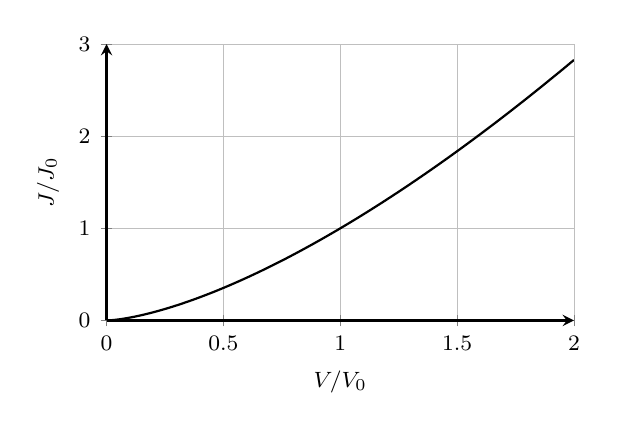
\begin{tikzpicture}
\begin{axis}[
 width=0.62\textwidth,
 height=0.42\textwidth,
 xlabel={$V/V_{0}$},
 ylabel={$J/J_{0}$},
 domain=0:2,
 samples=100,
 xmin=0, xmax=2,
 ymin=0, ymax=3,
 axis lines=left,
 thick,
 grid=both,
 grid style={line width=0.1pt, draw=gray!30},
 major grid style={line width=0.2pt, draw=gray!50},
 tick label style={font=\footnotesize},
 label style={font=\footnotesize},
]
\addplot[black, thick, domain=0:2, samples=100] {x^1.5};
\end{axis}
\end{tikzpicture}
\caption{Schematic, illustrative plot of the analytic Child--Langmuir scaling $J/J_{0} = (V/V_{0})^{3/2}$ of Eq.~\eqref{eq:annot:childlangmuir}. No experimental or simulated data are represented; the curve is included purely to fix the three-halves-power sheath scaling referenced throughout this appendix.}
\label{fig:annot:childlangmuir}
\end{figure}

\section{Methodological Synthesis}
\label{app:annot:synthesis}

The dependency structure linking the seven themes above runs strictly forward, since no single cited work spans the full chain from first-principles sheath theory to a validated erosion prediction. Section~\ref{app:annot:sheath-theory} fixes the boundary condition Eq.~\eqref{eq:annot:bohm} (or its magnetized form, Eq.~\eqref{eq:annot:bohmchodura}) that any admissible $f_{\mathrm{i}}(v)$ must satisfy at the sheath edge; Sec.~\ref{app:annot:ion-energy-flux} defines the moment of $f_{\mathrm{i}}(v)$, $\Gamma_{E}$ of Eq.~\eqref{eq:annot:gammaE}, the physically consequential output; Secs.~\ref{app:annot:lif-ivdf} and~\ref{app:annot:thomson} supply the two independent, non-perturbative measurement channels --- ion side and electron side --- from which $f_{\mathrm{i}}(v)$ and the boundary values entering Eq.~\eqref{eq:annot:bohm} are jointly constrained; Sec.~\ref{app:annot:inverse-problems} supplies the regularization apparatus, Eq.~\eqref{eq:annot:tikhonov}, without which neither channel's raw spectrum could be converted into an admissible estimate with defensible uncertainty; and Secs.~\ref{app:annot:hall-erosion} and~\ref{app:annot:fusion-pwi} close the loop by demonstrating, in two analogous settings, that $\Gamma_{E}$ so reconstructed governs the convex, threshold-sensitive surface response of Eq.~\eqref{eq:annot:erosion}. An error introduced at any stage --- an unmodelled deviation from Maxwellian electrons at the sheath-theory stage, or unaccounted broadening at the LIF stage --- therefore propagates multiplicatively rather than additively to the final prediction, because $\Gamma_{E}$ is a third-moment (velocity-cubed-weighted) integral of $f_{\mathrm{i}}(v)$ and is disproportionately sensitive to errors in the high-energy tail. This sensitivity is the principal justification for why an energy-\emph{resolved} estimator, rather than a mean-energy point estimate, is required wherever accurate erosion or heat-load prediction is the end goal.

\section{Summary}
\label{app:annot:summary}

The works annotated here trace a single continuous argument. The sheath-theory literature of Sec.~\ref{app:annot:sheath-theory} establishes the marginal ion speed $u_{\mathrm{B}}$ of Eq.~\eqref{eq:annot:bohm} and its kinetic, collisional, magnetized, and multi-species generalisations, fixing the boundary condition on $f_{\mathrm{i}}(v)$ at the sheath edge. Section~\ref{app:annot:ion-energy-flux} promotes this single-speed criterion to the full energy-resolved flux $\Gamma_{E}$ of Eq.~\eqref{eq:annot:gammaE}, the central quantity this monograph seeks to quantify. Sections~\ref{app:annot:lif-ivdf} and \ref{app:annot:thomson} supply the two principal non-perturbative diagnostic routes --- LIF for the ion side, Thomson scattering for the electron side --- while Sec.~\ref{app:annot:inverse-problems} supplies the regularization mathematics inverting noisy, line-integrated spectra into admissible profiles with quantified uncertainty. Finally, Secs.~\ref{app:annot:hall-erosion} and \ref{app:annot:fusion-pwi} demonstrate, in two analogous settings --- electric propulsion and magnetic confinement fusion --- that $\Gamma_{E}$, rather than the particle flux $\Gamma_{\mathrm{i}}$ alone, governs component erosion and lifetime via the threshold-like dependence expressed in Eq.~\eqref{eq:annot:erosion}. Read together, these seven themes justify both the theoretical construction and the diagnostic methodology this appendix supports.


\cleardoublepage
\phantomsection
\addcontentsline{toc}{part}{References}
\nocite{*}
\printbibliography[title={References},heading=bibintoc]

\end{document}
